\documentclass[11pt,oneside]{book}
\usepackage{fontspec}
\setmainfont{Noto Serif}
\setsansfont{Noto Sans}
\setmonofont{Noto Sans Mono}
\newfontfamily\proseunicodefont{DejaVu Serif}
\usepackage[margin=1in]{geometry}
\usepackage{microtype}
\usepackage{amsmath,amssymb,amsthm,mathtools,bm}
\usepackage{graphicx}
\usepackage{xcolor}
\usepackage{booktabs}
\usepackage{array}
\usepackage{longtable}
\usepackage{enumitem}
\usepackage{float}
\usepackage{caption}
\usepackage{hyperref}
\usepackage{fancyhdr}
\usepackage{tikz}
\usetikzlibrary{arrows.meta,positioning,calc,decorations.pathmorphing}

\hypersetup{
  colorlinks=true,
  linkcolor=blue!50!black,
  urlcolor=blue!50!black,
  citecolor=blue!50!black
}

\setlength{\parskip}{0.5em}
\setlength{\parindent}{0pt}
\setlist[itemize]{topsep=0.25em,itemsep=0.2em}
\setlist[enumerate]{topsep=0.25em,itemsep=0.2em}
\setlength{\headheight}{40pt}
\numberwithin{equation}{chapter}

\newtheorem{theorem}{Teorema}[chapter]
\newtheorem{proposition}[theorem]{Proposición}
\newtheorem{lemma}[theorem]{Lema}
\newtheorem{corollary}[theorem]{Corolario}
\theoremstyle{definition}
\newtheorem{definition}[theorem]{Definición}
\newtheorem{example}[theorem]{Ejemplo}
\theoremstyle{remark}
\newtheorem{remark}[theorem]{Observación}

\providecommand{\ket}[1]{\left\lvert#1\right\rangle}
\providecommand{\bra}[1]{\left\langle#1\right\rvert}
\providecommand{\braket}[2]{\left\langle#1\,\middle|\,#2\right\rangle}
\providecommand{\expect}[1]{\left\langle#1\right\rangle}
\newcommand{\lectureoverview}[1]{\paragraph{Resumen.} #1}
\newenvironment{classroomqa}{%
  \par\medskip
  \begin{quote}\small
}{%
  \end{quote}
  \medskip
}
\newcommand{\audiencequestion}[1]{\noindent\textbf{Pregunta del público.} #1\par\smallskip}
\newcommand{\classquestion}[1]{\noindent\textbf{Pregunta para la clase.} #1\par\smallskip}
\newcommand{\lecturerresponse}[1]{\noindent\textbf{Respuesta.} #1\par}
\newcommand{\lecturetimestamp}[1]{\footnote{Marca temporal: #1.}}
\newcommand{\lectureframe}[1]{\par\smallskip{\centering\footnotesize\itshape Fotograma de la clase: #1.\par}}

\makeatletter
\newcommand{\course@headerfont}{\normalfont\small\itshape}
\newcommand{\course@pagefont}{\normalfont\small}
\newcommand{\course@headerraise}{14pt}
\newlength{\course@headerboxheight}
\setlength{\course@headerboxheight}{\dimexpr\headheight-\course@headerraise-9pt\relax}
\newcommand{\course@leftheadbox}[1]{%
  \raisebox{\course@headerraise}{%
    \parbox[t][\course@headerboxheight][t]{0.82\textwidth}{%
      \raggedright\course@headerfont\strut\MakeUppercase{#1}\strut%
    }%
  }%
}
\newcommand{\course@rightheadbox}[1]{%
  \raisebox{\course@headerraise}{%
    \parbox[t][\course@headerboxheight][t]{0.82\textwidth}{%
      \raggedleft\course@headerfont\strut\MakeUppercase{#1}\strut%
    }%
  }%
}
\renewcommand{\chaptermark}[1]{\markboth{\MakeUppercase{\chaptername\ \thechapter.\ #1}}{}}
\renewcommand{\sectionmark}[1]{\markright{\MakeUppercase{\thesection\hspace{0.4em}#1}}}
\fancyhf{}
\fancyhead[L]{\course@leftheadbox{\leftmark}}
\fancyhead[R]{\course@pagefont\thepage}
\renewcommand{\headrulewidth}{0.5pt}
\pagestyle{fancy}
\fancypagestyle{plain}{%
  \fancyhf{}
  \fancyhead[L]{\course@leftheadbox{\leftmark}}
  \fancyhead[R]{\course@pagefont\thepage}
  \renewcommand{\headrulewidth}{0.5pt}
}
\makeatother

\usepackage{polyglossia}
\setdefaultlanguage{spanish}
\usepackage{sectsty}
\renewcommand{\contentsname}{Índice}
\renewcommand{\chaptername}{Capítulo}
\renewcommand{\figurename}{Figura}
\renewcommand{\tablename}{Tabla}
\renewcommand{\proofname}{Demostración}
\renewcommand{\bibname}{Bibliografía}
\sectionfont{\raggedright}
\subsectionfont{\raggedright}
\makeatletter
\renewcommand{\@pnumwidth}{2.2em}
\renewcommand{\@tocrmarg}{3.2em}
\makeatother
\usepackage{tocloft}
\renewcommand{\cftchapfont}{\small\bfseries}
\renewcommand{\cftchappagefont}{\small\bfseries}
\renewcommand{\cftsecfont}{\small}
\renewcommand{\cftsecpagefont}{\small}
\setlength{\cftsecnumwidth}{3em}
\renewcommand{\cftsubsecfont}{\small}
\renewcommand{\cftsubsecpagefont}{\small}
\setlength{\cftsubsecindent}{4.5em}
\setlength{\cftsubsecnumwidth}{4em}
\emergencystretch=6em
\pdfstringdefDisableCommands{\def\proseunicodefont{}}

\geometry{paperwidth=177.6mm,paperheight=252mm,left=16mm,right=16mm,
 top=18mm,bottom=18mm,includeheadfoot,headheight=28pt,headsep=7mm,footskip=9mm}
\usepackage{scrextend}
\changefontsizes[17pt]{12pt}
\raggedbottom
\renewenvironment{classroomqa}{\par\medskip\begingroup}{\par\endgroup\medskip}
\fancyhf{}
\setlength{\headwidth}{\textwidth}
\fancyhead[L]{\parbox{\textwidth}{\raggedright\fontsize{9}{11}\selectfont\nouppercase{\leftmark}}}
\fancyfoot[C]{\small\thepage}
\renewcommand{\headrulewidth}{0.3pt}
\fancypagestyle{plain}{\fancyhf{}\fancyfoot[C]{\small\thepage}\renewcommand{\headrulewidth}{0pt}}

\graphicspath{{../../../generated_course_notes/core/statistical_mechanics/2013_spring_theoretical_minimum/figures/}{../../../generated_course_notes/core/statistical_mechanics/2013_spring_theoretical_minimum/assets/}}
\hypersetup{
  pdftitle={Statistical Mechanics: The Theoretical Minimum},
  pdfauthor={Leonard Susskind; companion notes edited by LazyingArt LLC with Video2Book},
  pdfsubject={Core track, 2013 Spring},
  pdfkeywords={Leonard Susskind, statistical mechanics, thermodynamics, Ising model, critical phenomena}
}
\begin{document}
\frontmatter
\hypersetup{pageanchor=false}
\begin{titlepage}
\hyphenpenalty=10000\exhyphenpenalty=10000
\thispagestyle{empty}
\begin{tikzpicture}[remember picture,overlay]
  \node[anchor=south west,inner sep=0] at (current page.south west) {%
    \includegraphics[width=\paperwidth,height=\paperheight,keepaspectratio=false]{../../../generated_course_notes/core/statistical_mechanics/2013_spring_theoretical_minimum/assets/cover-art.png}%
  };
  \node[
    anchor=north west,
    align=left,
    text width=0.78\paperwidth,
    fill=white,
    fill opacity=0.9,
    rounded corners=8pt,
    inner xsep=10pt,
    inner ysep=8pt
  ] at ([xshift=0.08\paperwidth,yshift=-0.06\paperheight]current page.north west) {%
    {\fontsize{30}{33}\selectfont\bfseries\color{black!88} Mecánica estadística\\[0.85em]}
    {\large\color{black!72} Edición en español / primavera de 2013, mínimo teórico}
  };
  \node[
    anchor=south west,
    align=left,
    text width=0.68\paperwidth,
    fill=white,
    fill opacity=0.82,
    text opacity=1,
    rounded corners=6pt,
    inner sep=12pt
  ] at ([xshift=0.08\paperwidth,yshift=0.08\paperheight]current page.south west) {%
    {\normalsize\color{black!78} Clases originales: Leonard Susskind\\[0.35em]}
    {\small\color{black!72} Edición complementaria: \href{https://lazying.art}{LazyingArt LLC} / \href{https://github.com/lachlanchen/Video2Book}{Video2Book}.}
  };
\end{tikzpicture}
\mbox{}
\end{titlepage}
\hypersetup{pageanchor=true}

\chapter{Acerca de estas notas}
Estas notas complementarias, editadas de forma independiente, siguen las clases de 2013 de Mecánica estadística impartidas por Leonard Susskind. Conservan el orden explicativo de las clases, los intercambios sustantivos en el aula, las derivaciones matemáticas y una selección de pruebas de lo escrito en la pizarra. No son un manuscrito original del profesor Susskind, quien tampoco las ha revisado ni respaldado.

Esta edición fue preparada por \href{https://lazying.art}{LazyingArt LLC} mediante el flujo de trabajo de código abierto \href{https://github.com/lachlanchen/Video2Book}{Video2Book}. Las transcripciones automáticas completas y los archivos de subtítulos siguen disponibles por separado en el repositorio y pueden contener errores de reconocimiento.
\clearpage
\tableofcontents
\mainmatter
\chapter{Probabilidad, información y entropía}

\lectureoverview{La mecánica estadística comienza donde las leyes microscópicas se encuentran con el conocimiento incompleto. Primero damos precisión al concepto de probabilidad y luego preguntamos cómo el propio movimiento determinista asigna probabilidades, cómo las leyes de conservación dividen el espacio de estados y por qué la dinámica que conserva la información conduce de manera natural a la entropía. Las leyes primera y cero solo entran en escena una vez establecida esta estructura.}

\section{¿Por qué estudiar mecánica estadística?}

A veces se describe la mecánica estadística como física antigua. Esa descripción pasa por alto lo esencial. Es anterior a la modernidad, moderna y probablemente seguirá siendo útil en cualquier física posmoderna que suceda a las teorías que conocemos. Los modelos particulares aparecen y desaparecen; la segunda ley de la termodinámica ha sobrevivido repetidamente como guía. Siempre que una descripción propuesta de la naturaleza parezca generar orden de la nada, borrar información de forma fundamental o hacer que un sistema cerrado evolucione hacia un estado anormalmente simple, la segunda ley nos advierte que se ha dejado algo fuera.

El tema puede parecer menos fascinante que una partícula recién descubierta, pero es al menos igual de profundo y mucho más general. Los gases, los líquidos, los sólidos, la radiación, los agujeros negros, la información y los campos cuánticos requieren razonamiento estadístico. De hecho, no se podría entender la maquinaria experimental utilizada para descubrir partículas sin él. Por eso generaciones de físicos destacados dominaron la mecánica estadística incluso cuando su trabajo principal se desarrollaba en otros campos: el tema es útil, pero también posee una belleza excepcional.

Para ver por qué hace falta, partamos del ideal que ofrece la mecánica. Un sistema cerrado es el universo entero que se considera o un subsistema lo bastante aislado como para que su entorno no influya en él. Si conocemos su condición inicial y su ley de evolución, la mecánica clásica ofrece una predicción completa. La mecánica cuántica modifica lo que se puede predecir, pero también tiene un estado definido con precisión y una ley que predice la información máxima que permite la teoría.

Hay una diferencia profunda entre predecir en principio y comprender de manera útil. Una lista con la posición y la velocidad de cada molécula de esta habitación sería extraordinariamente larga, cambiaría casi de inmediato y respondería pocas de las preguntas que realmente nos interesan. Por tanto, las leyes microscópicas exactas pueden ser perfectamente predictivas y, al mismo tiempo, inútiles en la práctica.

La mecánica estadística es la teoría de la probabilidad aplicada a esta situación física. Se vuelve necesaria cuando no se conoce la condición inicial con exactitud perfecta, cuando la ley solo se conoce de manera aproximada, cuando el sistema es abierto o, sencillamente, cuando hay demasiadas variables microscópicas para seguirles la pista. Nada de esto implica que las predicciones sean poco precisas. A menudo, los números grandes hacen que las predicciones estadísticas sean extraordinariamente precisas.

Consideremos una caja aislada con gas. No podemos predecir la trayectoria de cada molécula, pero unos pocos datos macroscópicos nos permiten predecir con gran precisión la presión, la energía y muchas otras magnitudes macroscópicas. Lo que sigue siendo incierto son las fluctuaciones. En un momento impredecible, una región pequeña puede contener más moléculas que el promedio, mientras que otra contiene menos. Ese suceso se encuentra en la cola de una distribución de probabilidad: es improbable, pero no está prohibido. Podemos calcular con qué frecuencia deberían producirse tales fluctuaciones sin predecir el instante en que ocurrirá una en particular.

El lanzamiento de una moneda muestra la misma distinción. En mil millones de lanzamientos justos, los números de caras y cruces serán casi iguales. Si lanzamos la moneda suficientes veces, tarde o temprano aparecerá una larga racha de caras, pero la teoría de la probabilidad predice su frecuencia, no de antemano cuándo ocurrirá. La mecánica estadística está pensada para sistemas cuyos elementos son demasiado pequeños, demasiado numerosos o ambas cosas.

El curso desarrollará las leyes y sus aplicaciones a la materia. El tema recompensa el estudio reiterado: uno lo aprende, olvida algunas partes y vuelve a aprenderlo con una comprensión más profunda de cuáles ideas son fundamentales. Empezamos con la idea que rige todo lo que sigue.

\section{La probabilidad como lenguaje primitivo}

La razón por la que funciona la probabilidad no es algo que explique el propio cálculo de probabilidades. Una predicción probabilística puede fallar en un ensayo concreto; eso es lo que significa que un resultado sea posible, pero improbable. La teoría nos dice cómo se distribuyen las excepciones. No las elimina. Por eso tomamos la probabilidad como concepto primitivo y enunciamos las reglas que obedece.

\subsection{Estados y normalización}

Sea \(i\) la etiqueta de un resultado posible o de un estado posible de un sistema. Para una moneda, \(i\) puede representar cara o cruz. Para un dado, puede tomar valores desde \(1\) hasta \(6\). Para dos dados, un par de índices registra las dos caras. Empezamos con un espacio de estados discreto y finito,
\begin{equation}
 i=1,\ldots,N,
\end{equation}
y más adelante pasaremos a espacios con infinitos estados y a espacios con un continuo de estados.

La ignorancia no significa que el sistema carezca de estado. Significa que no sabemos cuál es su estado, así que asignamos una probabilidad \(p_i\) a cada posibilidad. Las reglas básicas son
\begin{align}
 p_i &\geq 0, \label{eq:sm1-prob-positive}\\
 \sum_{i=1}^{N}p_i &=1. \label{eq:sm1-prob-normalization}
\end{align}
Las alternativas son mutuamente excluyentes y exhaustivas: ocurre exactamente una de ellas. Aquí las probabilidades negativas no tienen cabida, y la suma es uno porque necesariamente ocurre algún resultado permitido.

\subsection{Frecuencia y ley de los grandes números}

La probabilidad se relaciona con el experimento mediante ensayos repetidos. Supongamos que se realiza \(N_{\mathrm{trials}}\) veces el mismo experimento y que \(N(i)\) es el número de ensayos que producen el resultado \(i\). Entonces, la interpretación frecuencial es
\begin{equation}
 p_i=
 \lim_{N_{\mathrm{trials}}\to\infty}
 \frac{N(i)}{N_{\mathrm{trials}}}.
 \label{eq:sm1-frequency}
\end{equation}
Se trata de una hipótesis física expresada mediante un límite ideal. Ningún laboratorio realiza infinitos experimentos. La afirmación es que, con suficientes ensayos, la razón se aproxima lo bastante a \(p_i\) para la predicción que se pretende hacer. Las muestras finitas fluctúan en torno al valor límite.

\subsection{Promedios}

Ahora asignemos un número \(f(i)\) a cada estado. Puede ser la energía, el momento u otra magnitud que queramos medir. Su valor esperado es
\begin{equation}
 \langle f\rangle=\sum_i f(i)p_i.
 \label{eq:sm1-expectation}
\end{equation}
La notación de corchetes resulta cómoda incluso fuera de la mecánica cuántica. En términos de frecuencias, el mismo promedio es
\begin{equation}
 \langle f\rangle
 =
 \lim_{N_{\mathrm{trials}}\to\infty}
 \frac{1}{N_{\mathrm{trials}}}
 \sum_i f(i)N(i).
 \label{eq:sm1-frequency-average}
\end{equation}

Para una moneda, definamos
\begin{equation}
 f(\mathrm{H})=+1,
 \qquad
 f(\mathrm{T})=-1.
\end{equation}
Si cara y cruz tienen cada una probabilidad \(1/2\), entonces
\begin{equation}
 \langle f\rangle
 =(+1)\frac12+(-1)\frac12=0.
\end{equation}
El promedio no tiene por qué ser un resultado posible. La moneda nunca cae en cero; el cero resume la distribución de sus dos valores posibles.

Esta breve digresión fija el vocabulario que se empleará en todo el tema: estados, probabilidades, frecuencias y valores esperados.

\section{Tres maneras de asignar probabilidades}

\subsection{Simetría}

¿Por qué solemos asignar probabilidades iguales a las dos caras de una moneda? La primera respuesta es la simetría. Al darle la vuelta a una moneda casi ideal se intercambian cara y cruz sin cambiar el experimento. En ese caso, no hay ninguna razón física para favorecer un resultado sobre el otro. Una marca o imperfección real introduce un pequeño sesgo, pero el modelo simétrico representa el experimento que se pretende describir:
\begin{equation}
 p(\mathrm{H})=p(\mathrm{T})=\frac12.
\end{equation}

El mismo razonamiento asigna probabilidad \(1/6\) a cada cara de un dado simétrico. En general, se asignan probabilidades iguales a las configuraciones relacionadas por una simetría, salvo que alguna información adicional rompa esa simetría.

\subsection{Experimento}

Un dado deforme no tiene ninguna simetría que intercambie sus seis caras. En ese caso, la simetría por sí sola no da una respuesta. Puede que tengamos un modelo mecánico más profundo que prediga el sesgo, pero, si no disponemos de él, el procedimiento honesto es experimental: lanzar el dado muchas veces, registrar las frecuencias, esperar a que se estabilicen y utilizar la tabla de probabilidades resultante en predicciones posteriores.

La simetría y el experimento no son definiciones que compitan entre sí. Son dos fuentes de información sobre una distribución de probabilidad. La mecánica estadística se apoyará mucho en la simetría, pero la dinámica ofrece una tercera vía.

\subsection{Probabilidad a partir del movimiento determinista}

Imaginemos un objeto irregular con seis configuraciones de colores. Cambia de estado a intervalos de tiempo discretos y regulares según una ley de actualización definida:
\begin{equation}
 R\longrightarrow B\longrightarrow Y\longrightarrow G
 \longrightarrow O\longrightarrow P\longrightarrow R.
 \label{eq:sm1-six-cycle}
\end{equation}
El objeto no tiene por qué poseer ninguna simetría geométrica. La ley solo especifica qué configuración sigue a una configuración dada.

\begin{figure}[htbp]
\centering
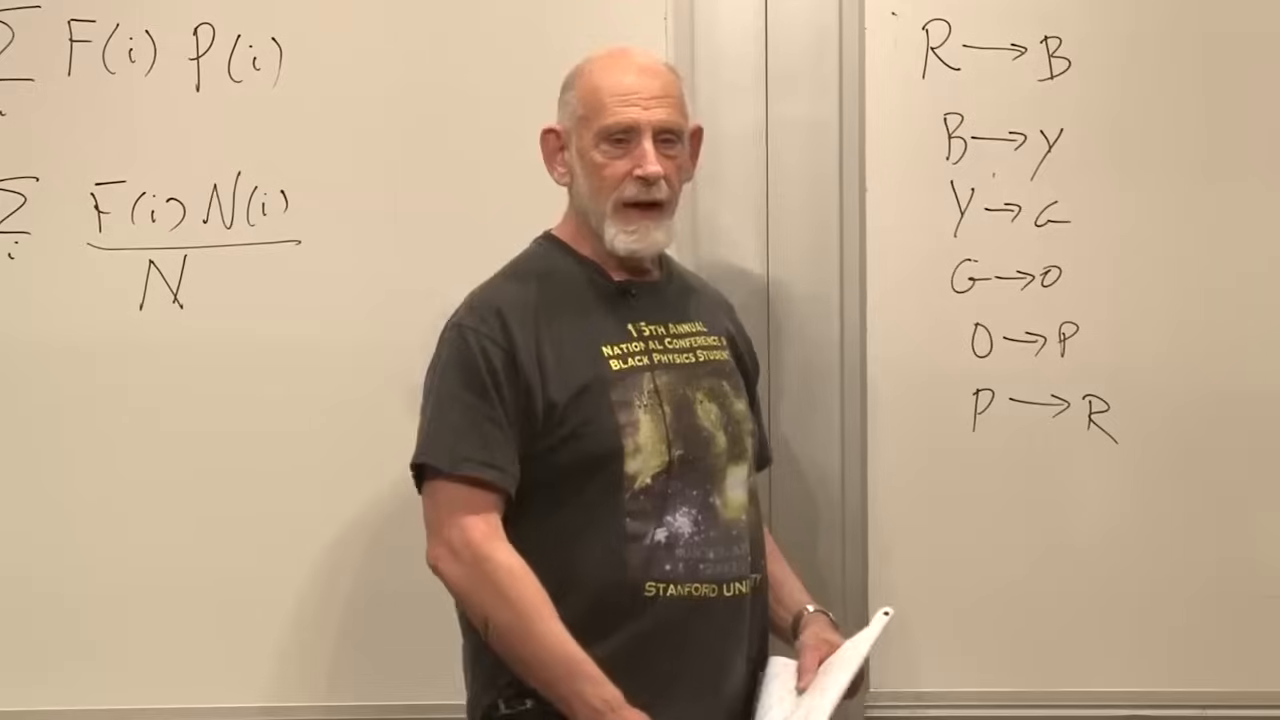
\includegraphics[width=0.92\textwidth]{lecture_01_figure_02.png}
\caption{Las fórmulas de los valores esperados permanecen en la pizarra de la izquierda, mientras que en la de la derecha se enumeran las seis actualizaciones deterministas de color.}
\lectureframe{00:26:28}
\end{figure}

La lista de la pizarra se entiende mejor si se representa como un ciclo dirigido:
\begin{figure}[htbp]
\centering
\begin{tikzpicture}[
  >=Latex,
  state/.style={draw,circle,minimum size=8mm,inner sep=1pt}
]
\node[state] (R) at (90:2.2) {$R$};
\node[state] (B) at (30:2.2) {$B$};
\node[state] (Y) at (-30:2.2) {$Y$};
\node[state] (G) at (-90:2.2) {$G$};
\node[state] (O) at (-150:2.2) {$O$};
\node[state] (P) at (150:2.2) {$P$};
\draw[->] (R) -- (B);
\draw[->] (B) -- (Y);
\draw[->] (Y) -- (G);
\draw[->] (G) -- (O);
\draw[->] (O) -- (P);
\draw[->] (P) -- (R);
\end{tikzpicture}
\caption{Una única órbita de seis estados. Cada estado se visita una vez durante cada período.}
\label{fig:sm1-six-cycle}
\end{figure}

Supongamos que desconocemos el estado inicial y tomamos una instantánea en un instante también desconocido. Como todos los pasos duran lo mismo, el sistema pasa una sexta parte del período en cada color:
\begin{equation}
 p(R)=p(B)=p(Y)=p(G)=p(O)=p(P)=\frac16.
 \label{eq:sm1-uniform-cycle}
\end{equation}
La igualdad no se debe a la forma del objeto. Se debe a que el tiempo transcurrido en cada estado es el mismo.

Podemos reordenar las flechas y obtener una ley microscópica distinta que siga formando un único ciclo de seis estados. La secuencia detallada cambia, pero la probabilidad de observar una instantánea sigue siendo \(1/6\), porque cada estado continúa apareciendo una vez por período. Por tanto, esta predicción no requiere conocer el punto de partida ni el orden detallado. Solo requiere la estructura de la órbita y el mismo tiempo para cada actualización.

\begin{classroomqa}
\classquestion{Si el objeto no es simétrico, ¿en qué sentido es
legítimo asignar a cada color una probabilidad \(1/6\)?}
\lecturerresponse{La asignación es dinámica, no geométrica. Una
instantánea tomada en una fase desconocida de una órbita de seis pasos muestrea seis intervalos de tiempo iguales. La equivalencia relevante es la de las posiciones en la órbita, no la de las caras del objeto. Si los tiempos de permanencia fueran distintos, las probabilidades también serían distintas.
\lecturetimestamp{00:27:11--00:29:49}}
\end{classroomqa}

\section{Ciclos desconectados y magnitudes conservadas}

Una ley determinista no tiene por qué situar todos los estados en una única órbita. Consideremos dos ciclos desconectados,
\begin{equation}
 R\longrightarrow B\longrightarrow G\longrightarrow R,
 \qquad
 P\longrightarrow Y\longrightarrow O\longrightarrow P.
 \label{eq:sm1-two-cycles}
\end{equation}
Si sabemos que el sistema está en el primer ciclo, entonces
\begin{equation}
 \begin{aligned}
 p(R)=p(B)=p(G)&=\frac13,\\
 p(P)=p(Y)=p(O)&=0.
 \end{aligned}
\end{equation}
Saber que está en el segundo ciclo invierte estas asignaciones.

El caso más general requiere pesos previos. Etiquetemos los ciclos con \(+1\) y \(-1\), y sean sus probabilidades \(p_+\) y \(p_-\), con
\begin{equation}
 p_++p_-=1.
\end{equation}
Entonces
\begin{align}
 p(R)=p(B)=p(G)&=\frac{p_+}{3},\\
 p(P)=p(Y)=p(O)&=\frac{p_-}{3}.
 \label{eq:sm1-sector-weights}
\end{align}
Los factores \(1/3\) se deben al movimiento dentro de cada ciclo. Los números \(p_+\) y \(p_-\) no. Deben provenir de información adicional, quizá de otro experimento o de otro sistema que seleccione el sector inicial.

Las etiquetas \(+1\) y \(-1\) definen una magnitud conservada: una vez que el sistema empieza en un ciclo, la ley de actualización nunca lo lleva al otro. Podemos llamar energía a esa magnitud o darle un nombre provisional como \emph{zilch}. El nombre es secundario. La conservación significa que el espacio de estados queda dividido en regiones que la dinámica no puede atravesar.

Los ciclos no tienen por qué contener el mismo número de estados. Una órbita de cuatro estados y otra de dos siguen definiendo dos sectores conservados. El muestreo con tiempos iguales da entonces \(1/4\) dentro del primero y \(1/2\) dentro del segundo, multiplicadas en ambos casos por la probabilidad previa de ese sector. La mecánica estadística debe responder a dos preguntas lógicamente distintas:
\begin{enumerate}
\item Dado un sector conservado, ¿cuánto tiempo pasa la dinámica en sus estados?
\item ¿Qué probabilidad debe asignarse al propio sector conservado?
\end{enumerate}

\begin{classroomqa}
\audiencequestion{¿Suponemos que todos los estados de un mismo
sector conservado reciben la misma probabilidad?}
\lecturerresponse{En las leyes discretas sencillas que se muestran aquí, sí, porque cada estado dura el mismo intervalo de tiempo y el movimiento es determinista. La incertidumbre está en la fase inicial de la órbita. Un detector con resolución temporal de milisegundos no puede resolver actualizaciones de microsegundos, aunque una instantánea lo bastante rápida aún puede identificar el estado que captó. En un sistema más general, deben tenerse en cuenta explícitamente los tiempos de permanencia desiguales.
\lecturetimestamp{00:36:16--00:37:17}}
\end{classroomqa}

\begin{classroomqa}
\audiencequestion{Si se toman dos instantáneas y la primera identifica un
ciclo, ¿debería la segunda identificar el mismo ciclo?}
\lecturerresponse{Sí. Eso es precisamente lo que significa la conservación. Una vez que una medición determina el valor de la magnitud conservada, las probabilidades futuras pueden condicionarse a ese valor, y a los estados del otro sector se les asigna probabilidad cero.
\lecturetimestamp{00:37:18--00:37:45}}
\end{classroomqa}

\subsection{Energía compartida entre dos sistemas}

Ahora reemplacemos la etiqueta abstracta por la energía. Una caja aislada es un sistema cerrado y tiene una energía conservada. Dos cajas aisladas tienen energías conservadas por separado porque no interactúan. Conectémoslas mediante un pasaje estrecho que permita el flujo de energía: las energías por separado pueden cambiar, pero la energía total permanece constante.

\begin{figure}[htbp]
\centering
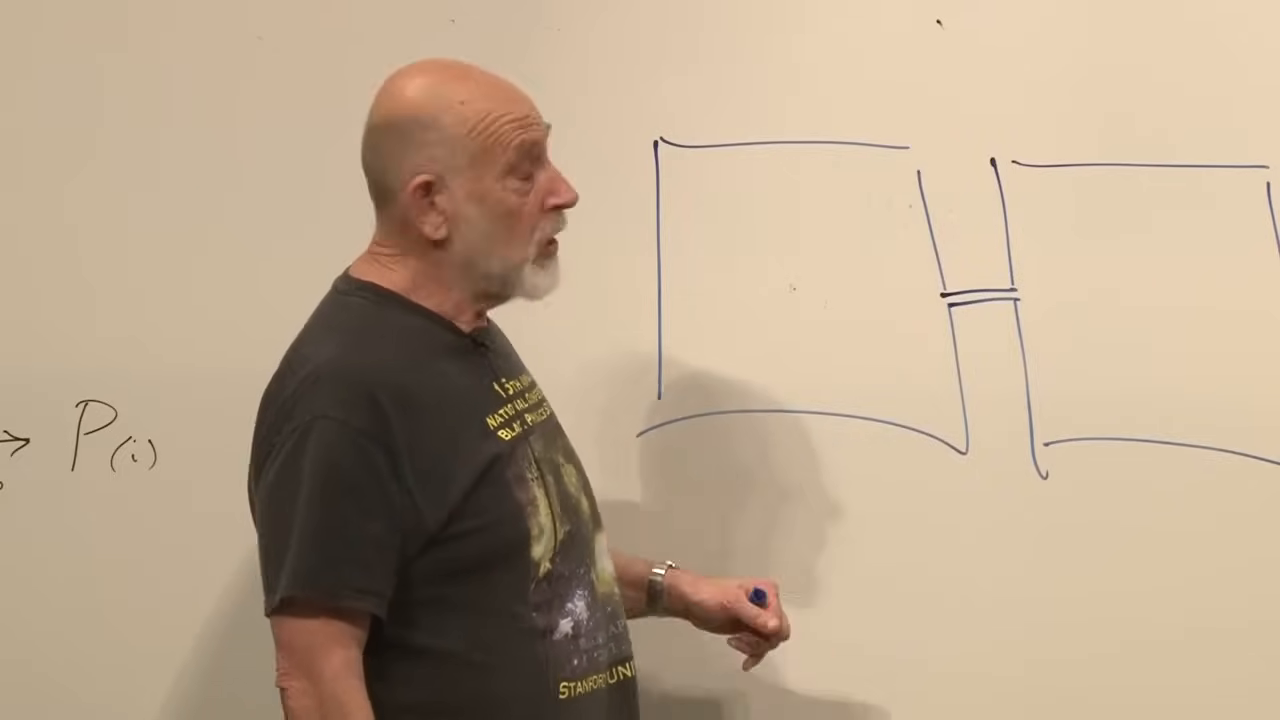
\includegraphics[width=0.92\textwidth]{lecture_01_figure_03.png}
\caption{Dos subsistemas conectados por un canal estrecho por el que puede pasar energía.}
\lectureframe{00:39:19}
\end{figure}

\begin{figure}[htbp]
\centering
\begin{tikzpicture}[>=Latex]
\draw[thick,rounded corners=4pt] (-4,1.8) rectangle (-0.7,-1.5);
\draw[thick,rounded corners=4pt] (0.7,1.5) rectangle (4,-1.8);
\draw[thick] (-0.7,0.45) -- (0.7,0.45);
\draw[thick] (-0.7,-0.35) -- (0.7,-0.35);
\draw[<->,very thick] (-0.45,0.05) -- (0.45,0.05);
\node at (-2.35,0.15) {subsystem \(1\)};
\node at (2.35,-0.15) {subsystem \(2\)};
\node[above] at (0,0.5) {energy exchange};
\end{tikzpicture}
\caption{Una vez abierta la conexión, solo se conserva \(E_1+E_2\). El reparto de energía se convierte en un problema de probabilidad.}
\label{fig:sm1-connected-systems}
\end{figure}

Dada una energía total, podemos preguntar cuál es la probabilidad de que el subsistema \(1\) tenga \(E_1\) y el subsistema \(2\) tenga el resto. Si las cajas son iguales, deberían tener la misma energía en promedio, pero el promedio no describe toda la distribución. Por tanto, una manera de determinar las probabilidades de un subsistema consiste en incluirlo en un sistema cerrado mayor cuya ley de conservación aporte la información que falta. Esta construcción reaparecerá a lo largo de la mecánica estadística.

\section{Leyes buenas, leyes malas y la ley menos uno}

No toda regla determinista de actualización es admisible como ley fundamental. Consideremos la aplicación
\begin{equation}
 \begin{aligned}
 R&\mapsto R,& B&\mapsto R,& Y&\mapsto R,\\
 G&\mapsto R,& O&\mapsto R,& P&\mapsto R.
 \end{aligned}
 \label{eq:sm1-all-to-red}
\end{equation}
Predice el futuro a la perfección: tras un paso, el estado es rojo. Falla en la dirección opuesta. Una vez que el sistema está en rojo, nada permite saber si llegó allí desde azul, amarillo, verde, naranja, morado o desde el propio rojo.

\begin{figure}[htbp]
\centering
\begin{tikzpicture}[
  >=Latex,
  state/.style={draw,circle,minimum size=8mm,inner sep=1pt}
]
\node[state,fill=red!12] (R) at (0,0) {$R$};
\node[state] (B) at (-3,1.6) {$B$};
\node[state] (Y) at (-3,0) {$Y$};
\node[state] (G) at (-3,-1.6) {$G$};
\node[state] (O) at (3,1.6) {$O$};
\node[state] (P) at (3,-1.6) {$P$};
\draw[->] (B) -- (R);
\draw[->] (Y) -- (R);
\draw[->] (G) -- (R);
\draw[->] (O) -- (R);
\draw[->] (P) -- (R);
\draw[->,loop above] (R) to (R);
\end{tikzpicture}
\caption{Una ley de muchos a uno predice el estado siguiente, pero borra las distinciones entre los posibles estados anteriores.}
\label{fig:sm1-bad-law}
\end{figure}

En cambio, un ciclo cerrado conserva el registro. Si conocemos el tiempo transcurrido, podemos hacer evolucionar el estado hacia adelante o hacia atrás, incluso después de muchos miles de períodos. La ley conserva las distinciones entre las condiciones iniciales. Susskind denomina a este requisito la \emph{ley menos uno de la física}: la información no se pierde de forma fundamental.

Para un espacio de estados discreto y finito, el criterio diagramático es sencillo:
\begin{quote}
Toda ley buena asigna exactamente una flecha saliente y exactamente una flecha entrante a cada estado.
\end{quote}
La flecha saliente determina el futuro; la entrante reconstruye el pasado. Matemáticamente, la actualización es una permutación de los estados.

\subsection{La fricción solo es un contraejemplo aparente}

La versión continua correspondiente es el teorema de Liouville. La fricción parece contradecirlo. Deslicemos una goma de borrar sobre una mesa: dondequiera que empiece, acaba deteniéndose. Una ecuación esquemática de arrastre es
\begin{equation}
 m\ddot x=-\gamma\dot x,
 \qquad \gamma>0.
 \label{eq:sm1-drag}
\end{equation}
Su velocidad decae exponencialmente. Si esta fuera la ley fundamental de todas las partículas de una habitación sellada, todo movimiento se extinguiría, la temperatura caería a cero y muchos estados iniciales convergerían en un único estado final. Fallaría la conservación de la energía, desaparecería información y disminuiría el desorden. Sería la versión continua de que todo se vuelve rojo.

La fricción real no funciona así. La goma calienta la mesa, a sí misma y al entorno. Las posiciones y los momentos microscópicos registran las distinciones que se pierden en el movimiento visible. La fricción es una ecuación efectiva para un subsistema, una vez omitidos los grados de libertad no observados; no es una ley fundamental disipativa para el sistema cerrado completo.

\begin{classroomqa}
\classquestion{¿Qué representa la ecuación diferencial
\(m\ddot x=-\gamma\dot x\) y por qué no es una ley fundamental para un
sistema cerrado?}
\lecturerresponse{Representa el arrastre viscoso. Por sí sola, hace que todas las velocidades tiendan a cero, lo que enfriaría un gas hasta cero cualquiera que fuera su temperatura inicial. En una descripción real de un sistema cerrado, la energía mecánica y la información perdidas pasan a los grados de libertad microscópicos. La ecuación de arrastre solo es fiable una vez que se han omitido esas variables.
\lecturetimestamp{00:44:40--00:48:56}}
\end{classroomqa}

\section{Estados ocupados y primera entropía}

La conservación de la información tiene un enunciado probabilístico equivalente. Supongamos que se asigna la misma probabilidad a \(M\) de los \(N\) estados,
\begin{equation}
 p_i=
 \begin{cases}
 1/M, & i\text{ in the occupied set},\\
 0, & i\text{ outside it}.
 \end{cases}
 \label{eq:sm1-uniform-occupied}
\end{equation}
Una actualización que conserva la información puede reorganizar los estados ocupados, pero no puede fusionarlos. En cualquier tiempo posterior siguen habiendo \(M\) estados con probabilidad \(1/M\). En cambio, la aplicación no adecuada \eqref{eq:sm1-all-to-red} puede hacer que muchos estados ocupados colapsen en uno solo.

El número \(M\) mide la ignorancia. Si \(M=N\), todos los estados son posibles y nuestra ignorancia es máxima. Si \(M=1\), se conoce exactamente el estado microscópico. Por tanto, la primera definición de entropía es
\begin{equation}
 S=\log M.
 \label{eq:sm1-entropy-logm}
\end{equation}
De ahí se obtiene
\begin{equation}
 S_{\max}=\log N,
 \qquad
 S_{\min}=0.
\end{equation}
Si el espacio de estados es infinito, puede no haber una cota superior finita.

En este desarrollo, la entropía aparece antes que la temperatura e incluso antes del enunciado formal de la conservación de la energía. En ese sentido, es más primitiva. Sin embargo, no es una propiedad exclusiva del sistema mecánico. Depende conjuntamente del sistema y de la distribución de probabilidad que representa lo que se conoce. Observadores con información distinta pueden asignar entropías distintas al mismo sistema mecánico.

Bajo una evolución microscópica exacta, los estados ocupados solo se reorganizan, por lo que esta entropía de grano fino se conserva. En la práctica, perdemos la información temporal, descartamos correlaciones y no conseguimos seguir la pista a cantidades enormes de variables. Entonces nuestra distribución de probabilidad se extiende sobre más alternativas y aumenta la entropía asignada a la descripción gruesa. Las ecuaciones no tienen por qué destruir la información para que nuestra descripción utilizable la pierda.

\begin{classroomqa}
\classquestion{¿Cuál es la entropía máxima posible de un sistema finito
con \(N\) estados?}
\lecturerresponse{Es \(\log N\), y se alcanza cuando los \(N\) estados tienen
la misma probabilidad. La entropía mínima es cero y se alcanza cuando un estado tiene probabilidad uno. Por tanto, la entropía mide tanto el estado del conocimiento como el espacio de estados disponible.
\lecturetimestamp{00:56:46--00:58:19}}
\end{classroomqa}

\section{Flujo de Liouville en el espacio de fases continuo}

Para partículas con posiciones y momentos continuos, un estado microscópico es un punto del espacio de fases. Escribimos las coordenadas como \(q_a\) y sus momentos conjugados como \(p_a\). Con muchas partículas hay un número enorme de ejes; un dibujo bidimensional con un \(q\) y un \(p\) es solo una representación esquemática. El espacio de fases es de dimensión par porque cada coordenada tiene un momento asociado.

Supongamos que nuestro conocimiento se representa mediante una región \(\Omega_0\): la densidad de probabilidad es uniforme dentro de ella y nula fuera. Por ejemplo, saber que todas las partículas están en la habitación restringe las coordenadas de posición, mientras que imponer límites a sus velocidades restringe las coordenadas de momento.

La evolución hamiltoniana hace que cada punto del espacio de fases siga una trayectoria. Los puntos próximos se transforman en puntos próximos, y la región ocupada fluye como una porción de fluido incompresible:
\begin{figure}[htbp]
\centering
\begin{tikzpicture}[>=Latex,scale=0.95]
\draw[->] (-4.2,0) -- (4.3,0) node[right] {$q$};
\draw[->] (-3.7,-2.2) -- (-3.7,2.4) node[above] {$p$};
\draw[fill=blue!12,thick]
  (-3.0,-0.5) .. controls (-2.7,1.0) and (-1.3,1.2) .. (-0.9,0.1)
  .. controls (-0.6,-1.0) and (-2.2,-1.4) .. cycle;
\node at (-1.9,0.0) {$\Omega_0$};
\draw[->,very thick] (-0.3,0.2) -- (0.8,0.2);
\draw[fill=orange!15,thick]
  (1.2,-1.1) .. controls (1.5,0.3) and (2.3,1.8) .. (3.2,1.1)
  .. controls (3.6,0.7) and (2.8,-0.4) .. (2.5,-1.5)
  .. controls (2.1,-1.8) and (1.5,-1.6) .. cycle;
\node at (2.35,0.1) {$\Omega_t$};
\end{tikzpicture}
\caption{El flujo hamiltoniano puede estirar y deformar por cizallamiento una región ocupada del espacio de fases, pero conserva su volumen.}
\label{fig:sm1-liouville-flow}
\end{figure}

El teorema de Liouville establece que
\begin{equation}
 \operatorname{Vol}(\Omega_t)
 =
 \operatorname{Vol}(\Omega_0).
 \label{eq:sm1-liouville-volume}
\end{equation}
Si la densidad inicial es uniforme en \(\Omega_0\), la densidad transportada es uniforme en \(\Omega_t\). Este es el análogo continuo de conservar el número y los pesos de los estados discretos ocupados.

El teorema también resuelve geométricamente el enigma de la fricción. Si solo observamos el momento visible de la goma, una nube de posibilidades parece contraerse hacia \(p=0\). En el espacio de fases completo, la nube se extiende por las posiciones y los momentos de las moléculas de la goma y de la mesa. Una proyección puede contraerse mientras el volumen total de alta dimensión permanece constante.

\begin{classroomqa}
\classquestion{Si todas las trayectorias visibles se acercan al reposo, ¿se ha
contraído la región ocupada del espacio de fases hasta el eje \(p=0\)?}
\lecturerresponse{Solo en la proyección reducida. El sistema completo
contiene las variables microscópicas de la mesa, la goma y el entorno. A medida que se estrecha el intervalo del momento visible, la distribución se extiende por esas direcciones ocultas. El teorema de Liouville se aplica al espacio de fases completo del sistema cerrado, no a un conjunto incompleto de variables macroscópicas.
\lecturetimestamp{01:04:37--01:06:29}}
\end{classroomqa}

\section{De la ley menos uno a la primera ley}

\subsection{Breve introducción a la ley cero}

Antes de enunciar la primera ley, conviene nombrar la ley cero. Aún no hemos definido el equilibrio térmico, así que por ahora la ley solo expresa una propiedad estructural:
\begin{quote}
Si el sistema \(A\) está en equilibrio térmico con \(B\), y \(B\) está en equilibrio térmico con \(C\), entonces \(A\) está en equilibrio térmico con \(C\).
\end{quote}
Esta transitividad permitirá definir la temperatura más adelante. Por ahora, la dejamos a un lado.

\subsection{Conservación de la energía}

La primera ley para un sistema cerrado es, sencillamente,
\begin{equation}
 \frac{dE}{dt}=0.
 \label{eq:sm1-first-law}
\end{equation}
Su forma compacta oculta su alcance. La energía es una magnitud conservada, y más adelante el término energía adquirirá un contenido termodinámico más amplio.

Si un sistema cerrado consta de dos partes y sus energías son aditivas,
\begin{equation}
 E=E_1+E_2,
\end{equation}
entonces
\begin{equation}
 \frac{dE_1}{dt}+\frac{dE_2}{dt}=0,
 \qquad\text{or}\qquad
 \frac{dE_1}{dt}=-\frac{dE_2}{dt}.
 \label{eq:sm1-energy-exchange}
\end{equation}
La segunda forma hace explícito el intercambio: la energía que pierde un subsistema la gana el otro.

La hipótesis de aditividad exige cuidado. Dos partículas que gravitan tienen energías cinéticas individuales, pero su interacción aporta una energía potencial que corresponde al par. La energía total se conserva, aunque no pueda escribirse exactamente como la energía de un cuerpo más la del otro.

En termodinámica suele ser posible una aproximación aditiva excelente, porque la energía macroscópica escala con el volumen, mientras que la energía de interacción de corto alcance entre piezas grandes vecinas depende principalmente del área de contacto. Dividamos una mesa grande en bloques: la energía interna de cada bloque es un efecto de volumen, mientras que el acoplamiento entre bloques adyacentes es un efecto superficial. En bloques grandes, este último es comparativamente pequeño. La ecuación \eqref{eq:sm1-first-law} es exacta para el conjunto cerrado; la forma para los subsistemas, \eqref{eq:sm1-energy-exchange}, supone que la energía de interacción es despreciable.

\begin{classroomqa}
\audiencequestion{¿La normalización \(\sum_i p_i=1\) también supone que los
resultados enumerados son mutuamente excluyentes?}
\lecturerresponse{Sí. Las etiquetas de estado se definen de modo que las alternativas no se solapen: si el dado está en el estado amarillo, no está simultáneamente en el rojo. En el lenguaje corriente pueden mezclarse los colores, pero la partición de estados empleada en el cálculo de probabilidades debe constar de alternativas mutuamente excluyentes.
\lecturetimestamp{01:12:14--01:12:55}}
\end{classroomqa}

\section{Volvamos a la entropía}

Ahora la lección vuelve explícitamente a lo que quedó pendiente. La temperatura, aunque nos resulte familiar a través de los sentidos, es una magnitud derivada. La entropía y la energía deben estar establecidas antes de poder definirla con claridad.

\subsection{Distribuciones de probabilidad generales}

La definición particular \(S=\log M\) se aplica cuando \(M\) estados tienen la misma probabilidad y todos los demás tienen probabilidad cero. Una distribución general no tiene por qué ser rectangular. Sus pesos pueden variar de forma suave o irregular a lo largo de las etiquetas de estado.

\begin{figure}[htbp]
\centering
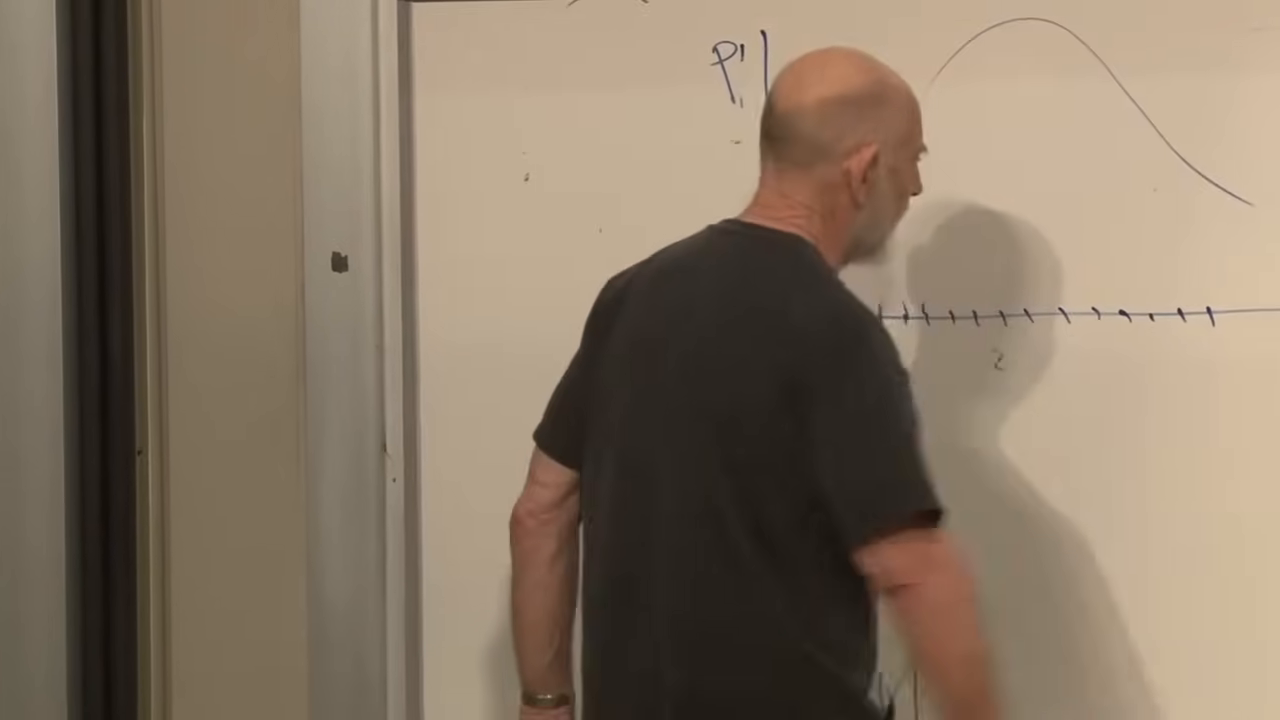
\includegraphics[width=0.92\textwidth]{lecture_01_figure_05.png}
\caption{Una distribución de probabilidad representada sobre etiquetas discretas de estado. Para la entropía, lo relevante es la dispersión, no la curva precisa.}
\lectureframe{01:14:40}
\end{figure}

\begin{figure}[htbp]
\centering
\resizebox{\linewidth}{!}{%
\begin{tikzpicture}[>=Latex,scale=0.93]
\draw[->] (-4.2,0) -- (4.4,0) node[right] {state label \(i\)};
\draw[->] (-4,0) -- (-4,3.2) node[above] {$p_i$};
\foreach \x in {-3.6,-3.1,...,3.6}
  \draw (\x,0.08) -- (\x,-0.08);
\draw[very thick]
  plot[smooth] coordinates {
  (-3.7,0.12) (-3.0,0.28) (-2.3,0.72) (-1.6,1.45)
  (-0.9,2.25) (-0.2,2.65) (0.5,2.28) (1.2,1.55)
  (1.9,0.88) (2.7,0.38) (3.5,0.14)};
\draw (-1.8,-0.18) -- (-1.8,-0.5);
\draw (1.8,-0.18) -- (1.8,-0.5);
\draw[<->] (-1.8,-0.46) -- (1.8,-0.46);
\node at (0,-0.82) {effective spread};
\end{tikzpicture}
}
\caption{Una distribución estrecha conlleva menos incertidumbre que una amplia. La entropía debe medir la distribución en su conjunto.}
\label{fig:sm1-probability-spread}
\end{figure}

La definición general es
\begin{equation}
 S=-\sum_i p_i\log p_i.
 \label{eq:sm1-shannon-entropy}
\end{equation}
Usando \eqref{eq:sm1-expectation}, se obtiene
\begin{equation}
 S=-\langle\log p\rangle.
\end{equation}
El signo menos compensa el hecho de que \(\log p_i<0\) cuando
\(0<p_i<1\).

\subsection{Recuperación del resultado uniforme}

Debemos comprobar que la fórmula general reproduce la primera definición.
Para un estado desocupado, \(p_i=0\) mientras que \(\log p_i\) diverge. El producto tiene el siguiente valor límite bien definido:
\begin{equation}
 \lim_{p\to0^+}p\log p=0.
 \label{eq:sm1-plogp-limit}
\end{equation}
Por tanto, los estados con probabilidad cero no contribuyen.

\begin{classroomqa}
\audiencequestion{Si \(p_i=0\), ¿el término realmente se anula? El logaritmo de cero es menos infinito.}
\lecturerresponse{El término se define mediante el límite
\(\lim_{p\to0^+}p\log p\), que es cero. El factor \(p\) tiende a cero más rápido de lo que diverge el logaritmo. Por tanto, los estados arbitrariamente improbables aportan cantidades arbitrariamente pequeñas, y un estado exactamente imposible no aporta nada.
\lecturetimestamp{01:18:27--01:19:46}}
\end{classroomqa}

Para cada uno de los \(M\) estados ocupados, \(p_i=1/M\). Por tanto,
\begin{align}
 S
 &=-\sum_{\mathrm{occupied}\ i}
 \frac1M\log\!\left(\frac1M\right)\\
 &=-M\frac1M\log\!\left(\frac1M\right)\\
 &=-\log\!\left(\frac1M\right)
 =\log M.
 \label{eq:sm1-entropy-check}
\end{align}
La expresión general coincide exactamente con la particular. Una distribución más amplia asigna un peso apreciable a más alternativas y, por tanto, tiene mayor entropía; una distribución más estrecha tiene menor entropía.

\begin{figure}[htbp]
\centering
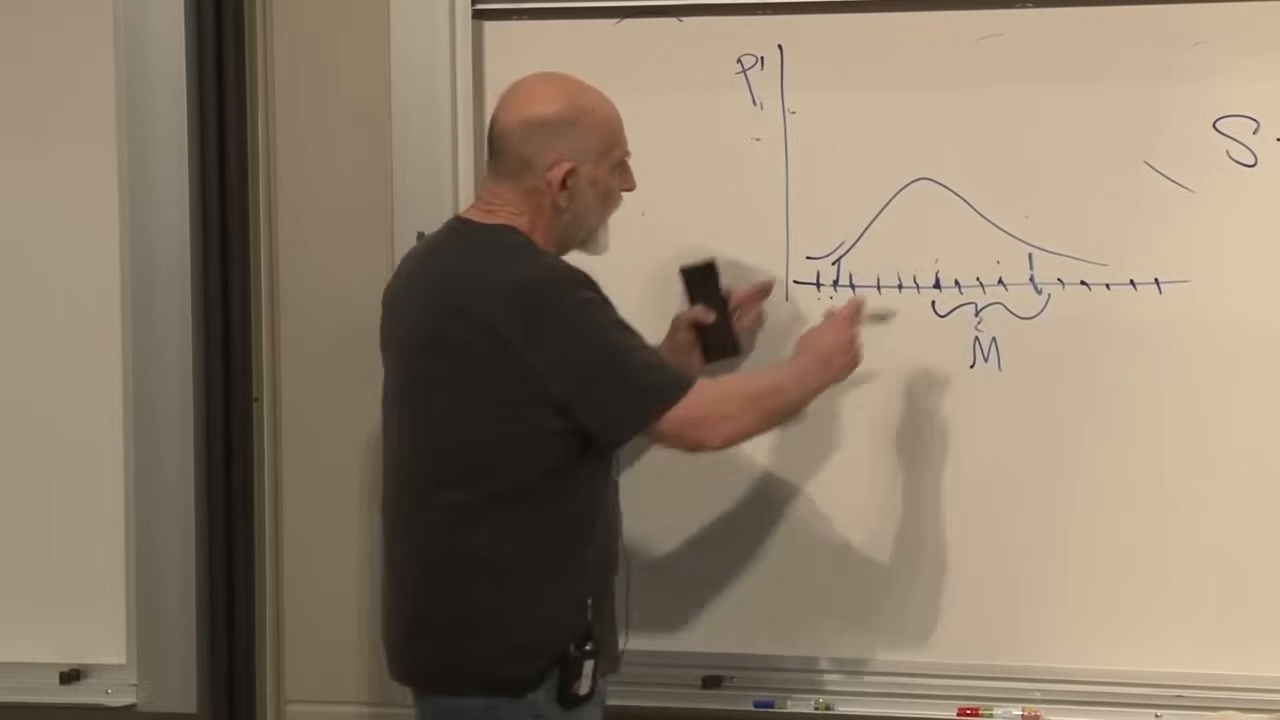
\includegraphics[width=0.92\textwidth]{lecture_01_figure_06.png}
\caption{La anchura indicada \(M\) resalta la relación entre la dispersión de las probabilidades significativas y la entropía.}
\lectureframe{01:16:42}
\end{figure}

La entropía corresponde a una distribución de probabilidad sobre el espacio de estados. No es una magnitud observable aislada, como la energía o el momento de un microestado. Un estado exacto puede representarse mediante una distribución concentrada en ese estado y, en tal caso, tiene entropía cero; sin embargo, la entropía cambia cuando cambia nuestro estado de conocimiento.

\section{Monedas, bits y recuento explícito}

Sea \(n\) el número de monedas. El número de configuraciones microscópicas es
\begin{equation}
 N=2^n.
 \label{eq:sm1-coin-state-count}
\end{equation}
Si no se sabe nada sobre las monedas, las \(2^n\) configuraciones son igualmente probables, y
\begin{equation}
 S_{\max}=\log(2^n)=n\log2.
 \label{eq:sm1-coin-max-entropy}
\end{equation}
La entropía es aditiva respecto al número de monedas independientes.

Con logaritmos en base \(2\), un sistema de dos estados completamente desconocido tiene una entropía de un bit. Con logaritmos naturales, su entropía es \(\log2\). La unidad es convencional; el orden subyacente y la aditividad no cambian.

En el otro extremo, si se conoce el resultado de cada moneda, una única configuración tiene probabilidad uno:
\begin{equation}
 S=0.
\end{equation}
Cuanto mayor es el conocimiento, menor es la entropía.

Supongamos ahora que exactamente una de las \(n\) monedas muestra cruz, todas las demás muestran cara y se desconoce la posición de la cruz. Hay \(n\) configuraciones igualmente probables, una por cada posición posible de la cruz, así que
\begin{equation}
 S=\log n.
 \label{eq:sm1-one-tail-entropy}
\end{equation}
En general, esto no es un múltiplo entero de \(\log2\). El bit es una unidad conveniente; no implica que toda entropía se presente en incrementos de bits enteros.

\begin{classroomqa}
\audiencequestion{¿Aparece \(\log2\) solo porque cada moneda tiene dos estados posibles? ¿Un elemento con tres estados daría \(\log3\)?}
\lecturerresponse{Exactamente. Un elemento con \(k\) estados posibles, todos igualmente desconocidos, aporta \(\log k\). Los interruptores binarios son especialmente convenientes en los ordenadores porque los interruptores físicos realizan de manera natural dos estados estables y porque dos es el menor entero no trivial.
\lecturetimestamp{01:29:55--01:30:48}}
\end{classroomqa}

\begin{classroomqa}
\audiencequestion{¿En qué base está definido el logaritmo?}
\lecturerresponse{En estas fórmulas de física, \(\log\) denota el logaritmo natural. Los teóricos de la información suelen usar la base \(2\), de modo que la entropía se mide directamente en bits. Cambiar la base multiplica todas las entropías por un mismo factor de conversión y no altera ninguna conclusión física.
\lecturetimestamp{01:30:49--01:32:06}}
\end{classroomqa}

\section{Entropía en el espacio de fases continuo}

Volvamos a un espacio de fases clásico \(\Gamma\). Si la densidad de probabilidad es uniforme en una región de volumen \(V_\Gamma\) y nula fuera de ella, el análogo de contar \(M\) estados igualmente probables es
\begin{equation}
 S=\log\!\left(\frac{V_\Gamma}{V_0}\right).
 \label{eq:sm1-continuous-uniform}
\end{equation}
Aquí \(V_\Gamma\) es el volumen en el espacio completo de coordenadas y momentos, de alta dimensión, no el volumen espacial ordinario. El volumen fijo \(V_0\) es una celda de referencia del espacio de fases que hace adimensional el argumento del logaritmo. Si se toma \(V_0=1\), se obtiene la forma abreviada \(S=\log V_\Gamma\) utilizada en la pizarra.

Para una densidad de probabilidad general \(P(q,p)\), la suma discreta se convierte en una integral sobre el espacio de fases. La normalización es
\begin{equation}
 \int_\Gamma d\Gamma\,P(q,p)=1,
 \label{eq:sm1-continuous-normalization}
\end{equation}
y la entropía es
\begin{equation}
 S=-\int_\Gamma d\Gamma\,
 P(q,p)\log\!\bigl[P(q,p)V_0\bigr].
 \label{eq:sm1-continuous-entropy}
\end{equation}
La densidad es la probabilidad por celda del espacio de fases. Conceptualmente, \eqref{eq:sm1-continuous-entropy} sigue midiendo cuán ampliamente se distribuye la probabilidad; para una distribución uniforme, se reduce al logaritmo del volumen ocupado medido en unidades de la celda de referencia. Cambiar esa celda fija desplaza todas las entropías continuas en la misma constante aditiva y deja inalteradas las diferencias de entropía.

\begin{classroomqa}
\audiencequestion{¿Por qué cambió el símbolo de coordenada de \(x\) a \(q\)?}
\lecturerresponse{No hay ningún cambio físico. En mecánica clásica se suele usar \(x\) o \(q\) para las coordenadas y \(p\) para los momentos conjugados. El cambio de notación fue solo un desliz; la construcción del espacio de fases es la misma.
\lecturetimestamp{01:37:10--01:37:39}}
\end{classroomqa}

La temperatura y la distribución de Boltzmann se dejan deliberadamente para más adelante. El siguiente paso será definir el equilibrio térmico y, después, identificar su distribución de probabilidad.

\section{Preguntas sobre correlación, aditividad e información}

\subsection{La correlación significa que una medición modifica otra distribución}

La ignorancia completa sobre monedas independientes asigna la misma probabilidad a todas las configuraciones. Medir una moneda no nos dice nada sobre ninguna de las otras. Sus distribuciones no cambian.

El conjunto de casos con una sola cruz es distinto. Si una moneda medida muestra cruz, todas las demás muestran necesariamente cara. Si la moneda medida muestra cara, la única cruz tiene que estar entre las \(n-1\) monedas restantes, así que cada posición restante tiene probabilidad condicionada
\begin{equation}
\begin{aligned}
 p(&\text{tail at a specified remaining position}\\
   &\mid\text{measured head})=\frac{1}{n-1}.
\end{aligned}
 \label{eq:sm1-conditional-tail}
\end{equation}
Esto es correlación: conocer una variable modifica la distribución de probabilidad asignada a otra.

\begin{classroomqa}
\audiencequestion{¿Se supuso que las monedas eran independientes en los ejemplos de entropía?}
\lecturerresponse{Solo cuando la ignorancia completa se representó asignando probabilidades iguales a las \(2^n\) configuraciones. En ese caso, medir una moneda no modifica las distribuciones de las demás. El ejemplo de una sola cruz tiene correlaciones explícitas: una medición actualiza lo que es posible en las otras posiciones. La información especificada determina qué distribución de probabilidad se utiliza.
\lecturetimestamp{01:38:43--01:41:58}}
\end{classroomqa}

El ejemplo del ciclo desconectado tiene la misma estructura lógica. Medir la etiqueta conservada \(+1\) o \(-1\) restringe todos los estados posteriores a un único sector. Condicionar por la información conservada cambia la distribución admisible.

La entropía es aditiva para sistemas no correlacionados. Si
\begin{equation}
 p_{ij}=p_i^{(A)}p_j^{(B)},
\end{equation}
entonces
\begin{align}
 S_{AB}
 &=-\sum_{i,j}p_i^{(A)}p_j^{(B)}
 \log\!\left[p_i^{(A)}p_j^{(B)}\right]\\
 &=S_A+S_B.
 \label{eq:sm1-entropy-additivity}
\end{align}
Las correlaciones impiden esta factorización y reducen la incertidumbre independiente del par.

Como ejercicio, imaginemos una fila de variables binarias en la que un estado arriba hace que cada vecino tenga una probabilidad de tres cuartos de estar abajo. Medir un sitio cambia de inmediato lo que se sabe sobre los sitios cercanos. Esa distribución está correlacionada, y su entropía no puede calcularse sumando las entropías de cada sitio por separado sin tener en cuenta esas correlaciones.

\subsection{Boltzmann, Shannon e incertidumbre cuántica}

\begin{classroomqa}
\audiencequestion{¿Qué relación hay entre la antigua entropía termodinámica y la entropía informacional de Shannon?}
\lecturerresponse{En ambas aparece la misma forma funcional:
\(-\sum_i p_i\log p_i\). Shannon solía usar la base \(2\), mientras que los físicos suelen usar logaritmos naturales y recuperan la constante de Boltzmann cuando expresan la entropía en unidades termodinámicas. La diferencia matemática consiste solo en un factor de conversión fijo, aunque las preguntas físicas que determinan las probabilidades pueden ser muy distintas.
\lecturetimestamp{01:44:05--01:46:06}}
\end{classroomqa}

Para microestados igualmente probables, la fórmula termodinámica suele escribirse como
\begin{equation}
 S_{\mathrm{thermo}}=k_{\mathrm B}\log W,
 \label{eq:sm1-boltzmann-formula}
\end{equation}
donde \(W\) es el número de microestados accesibles. En unidades en las que \(k_{\mathrm B}=1\), esto es precisamente \(S=\log W\). La constante de Boltzmann convierte entre unidades de temperatura y unidades de energía; la escala microscópica natural de la temperatura es la energía.

\begin{classroomqa}
\audiencequestion{¿Es esta entropía simplemente otra forma del principio de incertidumbre de Heisenberg?}
\lecturerresponse{No. La entropía que estamos considerando mide la incertidumbre de una distribución de probabilidad sobre estados posibles. En lenguaje cuántico, es la incertidumbre de un estado mixto, no la incertidumbre intrínseca de una medición que puede persistir incluso en un estado puro. Hay que distinguir claramente ambas nociones.
\lecturetimestamp{01:46:07--01:47:31}}
\end{classroomqa}

\section{Lo que se ha establecido}

El punto de partida no fue la aleatoriedad de las leyes. La dinámica determinista, combinada con un conocimiento incompleto del estado inicial, ya produce probabilidades. Una sola órbita asigna pesos según el tiempo que pasa en cada estado; las órbitas desconectadas revelan cantidades conservadas y requieren asignar pesos previos entre sectores. Las leyes microscópicas admisibles preservan las distinciones, lo que, en un espacio de estados finito, significa que en cada estado hay una flecha entrante y una saliente; en mecánica continua, esto se expresa mediante el teorema de Liouville.

Esa estructura conduce primero a
\begin{equation}
 S=\log M
\end{equation}
para \(M\) estados ocupados igualmente probables; después, a
\begin{equation}
 S=-\sum_i p_i\log p_i,
\end{equation}
y, finalmente, a su integral sobre el espacio de fases. La entropía registra una distribución de probabilidad y, por tanto, un estado de conocimiento. La ley microscópica conserva la información de grano fino, aunque una descripción práctica de grano grueso deje de seguirla.

La conservación de la energía da lugar a la primera ley, mientras que la aditividad de las energías de los subsistemas requiere que la energía de interacción sea despreciable. La entropía es aditiva bajo una condición análoga: las probabilidades de los subsistemas no deben estar correlacionadas. Estas dos formas de aditividad preparan el siguiente paso, en el que el equilibrio térmico, la temperatura y la distribución de Boltzmann relacionarán la energía con la probabilidad.

\chapter{Temperatura a partir de la entropía y la energía}

\lectureoverview{La temperatura aparece primero como una conversión de las unidades de los termómetros humanos a unidades de energía microscópica. Tras realizar la conversión correspondiente de la entropía termodinámica a la entropía estadística adimensional, describimos el equilibrio mediante una familia uniparamétrica de distribuciones de probabilidad. La derivada \(dE/dS\) define entonces la temperatura, y las dos primeras leyes muestran por qué una diferencia de temperatura determina el sentido del flujo de energía.}

\section{Factores de conversión y unidades humanas}

Muchas constantes de la física son factores de conversión. La velocidad de la luz convierte una distancia en un tiempo:
\begin{equation}
 t=\frac{x}{c}.
\end{equation}
Si las distancias y los tiempos se miden en unidades compatibles, se puede fijar \(c=1\). No desaparece ningún efecto físico; simplemente se han expresado ambos tipos de medida en una escala común.

La constante de Boltzmann tiene el mismo carácter. Convierte la temperatura que indica un termómetro en una escala humana en energía. El adjetivo \emph{de escala humana} es importante. Estas unidades se eligen porque los instrumentos macroscópicos pueden producirlas y resolverlas, no porque la dinámica microscópica las distinga de manera especial.

El grado Celsius se fijó dividiendo en cien partes el intervalo entre los puntos de congelación y ebullición del agua a presión estándar. El kelvin usa un grado del mismo tamaño, pero sitúa el cero en el cero absoluto. Elegir otra sustancia, otro intervalo o grados Fahrenheit cambiaría los números, pero no la física.

\begin{classroomqa}
\audiencequestion{¿La escala Fahrenheit ya se había creado en el siglo XVII?}
\lecturerresponse{Aquí no hace falta precisar la fecha. Lo importante es que todas esas escalas se diseñaron en torno a temperaturas que las personas podían alcanzar y medir. El tamaño de sus grados es convencional, no microscópico.
\lecturetimestamp{00:01:34--00:01:50}}
\end{classroomqa}

Cuando se crearon estas escalas, el origen molecular del calor aún no estaba al alcance de la experimentación. Un termómetro macroscópico podía detectar un cambio de un grado, mientras que no se podía medir la energía de una sola molécula. Por eso era natural inventar una unidad de temperatura antes de saber que, en el fondo, la temperatura es una escala de energía.

\section{Por qué la temperatura tiene unidades de energía}

Consideremos un gas monoatómico diluido. Que sea diluido significa que, para lo que nos interesa ahora, podemos despreciar las energías de interacción entre moléculas. En equilibrio térmico, la equipartición asigna \(T_{\mathrm K}/2\) veces la constante de Boltzmann a cada grado de libertad traslacional cuadrático. En tres dimensiones espaciales,
\begin{equation}
 \left\langle E_{\mathrm{kin}}\right\rangle
 =\frac{3}{2}k_{\mathrm B}T_{\mathrm K}.
 \label{eq:sm2-equipartition-kelvin}
\end{equation}
El factor tres cuenta el movimiento en las direcciones \(x\), \(y\) y \(z\). El factor un medio procede de la energía cinética cuadrática.

Esta relación no es exclusiva de una especie molecular. En una mezcla de helio y oxígeno en equilibrio, todas las partículas con traslación libre tienen la misma energía cinética media del centro de masas, aunque las partículas más pesadas se muevan más despacio. Como
\begin{equation}
 E_{\mathrm{kin}}=\frac{1}{2}mv^2,
\end{equation}
a igual energía característica le corresponde \(v\propto m^{-1/2}\).

La misma idea puede llevarse a un ejemplo deliberadamente extremo. Suspendamos una bola de bolos en un fluido y dejemos que el sistema completo alcance el equilibrio. Sus grados de libertad traslacionales brownianos están regidos por la misma escala de energía que los de una molécula. La velocidad de la bola es extraordinariamente menor porque su masa es extraordinariamente mayor, pero la temperatura compara escalas de energía, no velocidades.

A temperatura ambiente, \(T_{\mathrm K}\) es aproximadamente \(300\,\mathrm K\), mientras que la energía de un grado de libertad microscópico es ínfima en julios. Por consiguiente, el factor de conversión es muy pequeño:
\begin{equation}
 k_{\mathrm B}\simeq 1.38\times10^{-23}\,
 \mathrm{J\,K^{-1}}.
 \label{eq:sm2-boltzmann-value}
\end{equation}
Su escala y el número de Avogadro están relacionados; no es una coincidencia:
\begin{equation}
 R=N_{\mathrm A}k_{\mathrm B}.
\end{equation}
La constante de los gases \(R\) describe un mol, mientras que \(k_{\mathrm B}\) describe la escala correspondiente por constituyente microscópico.

La combinación \(k_{\mathrm B}T_{\mathrm K}\) aparece una y otra vez en las fórmulas fundamentales. Por eso es más sencillo definir
\begin{equation}
 T\equiv k_{\mathrm B}T_{\mathrm K}.
 \label{eq:sm2-energy-temperature}
\end{equation}
A partir de ahora \(T\) tiene unidades de energía, y \eqref{eq:sm2-equipartition-kelvin} pasa a ser
\begin{equation}
 \left\langle E_{\mathrm{kin}}\right\rangle=\frac{3}{2}T.
 \label{eq:sm2-equipartition-natural}
\end{equation}
Si la energía se mide en julios, la temperatura se mide en julios. Si la energía se mide en electronvoltios, la temperatura se mide en electronvoltios. No existe ninguna nueva unidad natural llamada unidad de temperatura.

\section{Dos convenciones para la entropía}

La misma conversión aparece en el caso de la entropía. La termodinámica macroscópica surgió del análisis de las máquinas térmicas. Carnot aportó el razonamiento decisivo sobre las máquinas; más tarde, Clausius introdujo la entropía termodinámica y el símbolo \(S\). En la notación que usaremos aquí, llamemos \(S_{\mathrm C}\) a esa magnitud macroscópica. Sus unidades son energía dividida por temperatura indicada por un termómetro, por ejemplo, julios por kelvin.

La entropía estadística es adimensional. Para una distribución discreta,
\begin{equation}
 S=-\sum_i p_i\log p_i.
 \label{eq:sm2-statistical-entropy}
\end{equation}
Con logaritmos naturales, una alternativa binaria equiprobable tiene entropía \(\log2\); con logaritmos en base dos, esa misma cantidad se denomina un bit. Las dos convenciones para la entropía están relacionadas por
\begin{equation}
 S=\frac{S_{\mathrm C}}{k_{\mathrm B}},
 \qquad
 S_{\mathrm C}=k_{\mathrm B}S.
 \label{eq:sm2-entropy-conversion}
\end{equation}
Un valor macroscópico moderado en \(\mathrm{J\,K^{-1}}\) corresponde a una entropía adimensional enorme, porque cuenta información distribuida entre un número enorme de constituyentes microscópicos.

Las ecuaciones \eqref{eq:sm2-energy-temperature} y \eqref{eq:sm2-entropy-conversion} establecen la convención que usaremos en todo el texto:
\[
 [T]=[\text{energy}],
 \qquad
 [S]=1.
\]
La constante de Boltzmann puede desaparecer ahora de las fórmulas de trabajo. Siempre se puede reintroducir reemplazando \(T\) por \(k_{\mathrm B}T_{\mathrm K}\) y \(S\) por \(S_{\mathrm C}/k_{\mathrm B}\).

\begin{classroomqa}
\audiencequestion{Aparte del factor \(3/2\), ¿la nueva temperatura es simplemente una energía medida en julios?}
\lecturerresponse{Sí, si se eligen los julios como unidad de energía. El julio es la unidad MKS \(\mathrm{kg\,m^2\,s^{-2}}\). También se podrían usar electronvoltios o cualquier otra unidad de energía; en tal caso, la temperatura tendría que expresarse en esa misma unidad. El factor \(3/2\) corresponde al ejemplo del gas ideal, no a la definición de temperatura.
\lecturetimestamp{00:15:49--00:16:45}}
\end{classroomqa}

\begin{classroomqa}
\audiencequestion{Si el pizarrón especifica kelvin, ¿no es entonces \(k_{\mathrm B}\) una constante definida?}
\lecturerresponse{Queda definida una vez especificadas tanto la unidad de temperatura como la de energía. Si se cambia el kelvin por grados Fahrenheit, o los julios por electronvoltios, cambia su valor numérico. Esa dependencia de las unidades es precisamente la que caracteriza a un factor de conversión.
\lecturetimestamp{00:16:46--00:18:33}}
\end{classroomqa}

\begin{classroomqa}
\audiencequestion{¿Se determina experimentalmente el valor numérico de la constante de Boltzmann?}
\lecturerresponse{Sí. Históricamente, para evaluarla se necesitaba información microscópica sobre los átomos y su densidad numérica. Boltzmann entendió la relación entre la energía molecular y la temperatura antes de que esas magnitudes se conocieran con precisión, de manera parecida a como Newton conocía el papel de la constante gravitatoria antes de que se midiera con exactitud.
\lecturetimestamp{00:18:46--00:20:00}}
\end{classroomqa}

\section{El equilibrio es un estado estadístico}

La conversión de unidades todavía no ha definido la temperatura. Tocar algo caliente ofrece una intuición biológica útil, pero la temperatura es una magnitud física derivada, construida a partir de la energía y la entropía.

Imaginemos un sistema en contacto con un entorno grande cuyas condiciones macroscópicas se mantienen fijas. Puede intercambiar energía con él. Si al principio el sistema tiene demasiada energía, en promedio la pierde; si tiene muy poca, en promedio la gana. En equilibrio térmico siguen produciéndose intercambios microscópicos, pero el flujo neto medio en cualquiera de los dos sentidos es nulo.

Sea \(i\) la etiqueta de un estado microscópico exacto del sistema, y sea \(E_i\) la energía de ese estado. El equilibrio no significa que el sistema quede inmóvil en un único estado. La interacción con el entorno cambia continuamente el microestado, así que asignamos una probabilidad \(P_i\) a cada posibilidad. Las relaciones básicas son
\begin{align}
 \sum_i P_i &=1,
 \label{eq:sm2-normalization}\\
 \sum_i P_iE_i &=\overline E,
 \label{eq:sm2-mean-energy}\\
 S&=-\sum_iP_i\log P_i.
 \label{eq:sm2-equilibrium-entropy}
\end{align}
La barra sobre \(\overline E\) destaca que la energía del subsistema fluctúa. Una medición puede dar un valor y la siguiente, otro; al repetir las mediciones, se obtiene la distribución cuya media es \eqref{eq:sm2-mean-energy}.

\begin{figure}[t]
\centering
\includegraphics[width=0.82\textwidth]{lecture_02_figure_02.png}
\caption{Normalización y energía media en el pizarrón: \(\sum_iP(i)=1\) y \(\sum_iP(i)E(i)=\langle E\rangle\).}
\lectureframe{00:24:10}
\end{figure}

\section{Una familia parametrizada por la energía media}

La distribución de equilibrio depende mucho de la energía media. Si ponemos una olla de agua al fuego, \(\overline E\) aumenta; si la dejamos en la nieve, \(\overline E\) disminuye. Las probabilidades cambian con ella. Por tanto, el equilibrio debe entenderse no como una sola distribución, sino como una familia uniparamétrica:
\begin{equation}
 P_i(\overline E).
 \label{eq:sm2-family}
\end{equation}
Cada miembro satisface
\begin{align}
 \sum_iP_i(\overline E)&=1,
 \label{eq:sm2-family-normalization}\\
 \sum_iP_i(\overline E)E_i&=\overline E.
 \label{eq:sm2-family-mean}
\end{align}

\begin{figure}[t]
\centering
\includegraphics[width=0.88\textwidth]{lecture_02_figure_03.png}
\caption{La transición a \(P(i,\overline E)\). Las ecuaciones anteriores de normalización, energía media y entropía permanecen visibles mientras se introduce la familia de distribuciones.}
\lectureframe{00:26:29}
\end{figure}

Para un gráfico esquemático, ordenemos los estados según el valor creciente de \(E_i\). Así, el eje horizontal puede leerse como el índice \(i\) o como la energía correspondiente. Una energía media mayor desplaza el peso de probabilidad hacia los estados situados más a la derecha. El área total bajo cada curva debe ser igual a uno.

\begin{figure}[t]
\centering
\includegraphics[width=0.88\textwidth]{lecture_02_figure_04.png}
\caption{Varias distribuciones esquemáticas \(P(i,\overline E)\). Las curvas con más peso hacia la derecha tienen mayor energía media, y todas están normalizadas.}
\lectureframe{00:28:40}
\end{figure}

\begin{figure}[t]
\centering
\begin{tikzpicture}[x=1cm,y=1cm]
\draw[->] (0,0) -- (7.4,0) node[right] {$E_i$};
\draw[->] (0,0) -- (0,3.25) node[above] {$P_i(\overline E)$};
\draw[thick,blue!70!black]
  plot[smooth] coordinates {(0,0) (0.35,1.6) (0.85,2.65) (1.45,1.45)
  (2.2,0.35) (3.0,0)};
\draw[thick,teal!70!black]
  plot[smooth] coordinates {(0,0) (0.7,0.7) (1.5,1.7) (2.5,2.0)
  (3.7,0.8) (4.8,0)};
\draw[thick,orange!80!black]
  plot[smooth] coordinates {(0,0) (1.3,0.3) (2.7,0.9) (4.3,1.45)
  (5.8,0.85) (7.0,0)};
\node[blue!70!black] at (1.0,2.95) {\(\overline E_1\)};
\node[teal!70!black] at (2.75,2.3) {\(\overline E_2\)};
\node[orange!80!black] at (5.2,1.7) {\(\overline E_3\)};
\node at (4.9,2.85) {\(\overline E_1<\overline E_2<\overline E_3\)};
\end{tikzpicture}
\caption{Una versión limpia del esquema del pizarrón. No hace falta que las curvas tengan estas formas precisas; solo se usan la normalización y el orden de sus energías medias.}
\end{figure}

\begin{classroomqa}
\audiencequestion{¿Es circular esta notación? La energía media se calcula a partir de la distribución, pero la distribución está parametrizada por la energía media.}
\lecturerresponse{Partamos de una familia uniparamétrica de distribuciones de equilibrio elegida empíricamente. Cada miembro tiene una energía media. Si miembros distintos tienen medias distintas, se puede usar esa media como parámetro para nombrar la familia. La notación todavía no deriva la familia; más adelante, la distribución de Boltzmann proporcionará esa derivación.
\lecturetimestamp{00:28:35--00:29:44}}
\end{classroomqa}

\begin{classroomqa}
\audiencequestion{¿Por qué se habla de energía media y no de energía total?}
\lecturerresponse{El subsistema intercambia energía con un baño térmico, como la atmósfera que rodea un recipiente de gas cuyas paredes dejan pasar el calor. Su energía instantánea fluctúa. Al hacer muchas mediciones se obtiene una distribución, y \(\overline E\) es la media de esos resultados. La energía del sistema cerrado más grande, formado por el subsistema y el baño, sí puede mantenerse fija.
\lecturetimestamp{00:29:46--00:30:56}}
\end{classroomqa}

\begin{classroomqa}
\audiencequestion{¿Pueden tener la misma energía distintos estados microscópicos? ¿Y pueden tener la misma energía media distintas distribuciones?}
\lecturerresponse{Ambas cosas son posibles. La condición sobre la energía media, por sí sola, permite muchas distribuciones, así que hace falta otro argumento físico para obtener la familia uniparamétrica especial de equilibrio. Más adelante se derivarán su origen y su forma de Boltzmann. Que distintos microestados tengan la misma energía es otra cuestión, denominada degeneración.
\lecturetimestamp{00:30:58--00:32:22}}
\end{classroomqa}

\subsection{Etiquetas de estado, degeneración y correlación}

Hay que mantener separados varios conceptos que se confunden con facilidad.

Primero, muchas distribuciones de probabilidad pueden tener la misma energía media. La familia uniparamétrica de equilibrio no se obtiene únicamente de la condición sobre la energía media. Es la familia particular que selecciona la equilibración; más adelante veremos que su forma es la distribución de Boltzmann.

Segundo, varios microestados distintos pueden tener la misma energía. Esto se llama degeneración. En el análisis del pizarrón, por el momento se ignoran las degeneraciones exactas para poder ordenar los estados sin ambigüedad según su energía. De hecho, la degeneración es común cuando un sistema tiene simetrías, pero no plantea ningún problema conceptual: se conserva la etiqueta del estado \(i\), se permiten valores repetidos de \(E_i\) y se suman todos los estados.

Tercero, correlación no es otra manera de decir degeneración. La correlación concierne a una distribución conjunta de dos magnitudes aleatorias y pregunta si conocer una modifica las probabilidades de la otra. Las etiquetas mutuamente excluyentes \(i\) y \(j\) en una lista de microestados no son, por sí solas, dos variables aleatorias cuya correlación se esté calculando.

\begin{classroomqa}
\audiencequestion{¿La construcción supone que los distintos estados \(i\) son independientes? ¿Y qué ocurre si dos de ellos están correlacionados?}
\lecturerresponse{Una etiqueta de estado es un valor posible de una sola variable aleatoria microscópica. La independencia y la correlación requieren dos variables con una distribución conjunta, así que esos términos no se aplican directamente a dos etiquetas alternativas de esta lista. Que distintos estados tengan la misma energía es, en cambio, una cuestión de degeneración.
\lecturetimestamp{00:32:23--00:33:22}}
\end{classroomqa}

\begin{classroomqa}
\audiencequestion{¿Qué ocurre si dos estados distintos tienen exactamente la misma energía?}
\lecturerresponse{Eso es degeneración. Para el gráfico inmediato adoptamos la simplificación de suponer que no coinciden dos energías y ordenamos los estados por energía creciente. Las fórmulas de probabilidad que obtendremos más adelante no requieren esta suposición; los estados degenerados simplemente se cuentan por separado.
\lecturetimestamp{00:33:23--00:34:04}}
\end{classroomqa}

\begin{classroomqa}
\audiencequestion{¿Es arbitrario el significado del índice \(i\)?}
\lecturerresponse{Los estados microscópicos en sí no son arbitrarios: cada uno especifica todas las posiciones, los momentos u otros datos necesarios para una descripción exacta. Sus nombres sí son arbitrarios, así que para la figura elegimos etiquetas en orden creciente de energía.
\lecturetimestamp{00:34:06--00:35:15}}
\end{classroomqa}

\section{La entropía pasa a ser una función de la energía}

Cada miembro de la familia de equilibrio tiene una entropía. Al sustituir \eqref{eq:sm2-family} en \eqref{eq:sm2-equilibrium-entropy} se obtiene
\begin{equation}
 S(\overline E)
 =-\sum_iP_i(\overline E)\log P_i(\overline E).
 \label{eq:sm2-entropy-energy}
\end{equation}
No se trata de una función universal común a todos los sistemas físicos. Depende del espectro del sistema y de su familia de equilibrio. Sin embargo, una vez especificada esa familia, la energía y la entropía quedan vinculadas: al recorrerla, ambas cambian.

En los sistemas ordinarios, la probabilidad suele repartirse entre más estados a medida que aumenta la energía media; por eso, \(S\) suele aumentar con \(\overline E\). Por ahora suponemos que esta relación es suave e invertible localmente. Las excepciones son importantes, pero el caso sencillo permite presentar la definición que necesitamos.

\section{La derivada que define la temperatura}

Planteemos una pregunta concreta: ¿cuánto debe cambiar la energía media para aumentar la entropía en una alternativa binaria? En unidades de logaritmo natural, ese incremento de entropía es \(\log2\).

Para miembros cercanos de una familia suave,
\begin{equation}
 dE=\frac{dE}{dS}\,dS.
 \label{eq:sm2-differential-identity}
\end{equation}
Por ahora, la ecuación no es más que la regla de la cadena. Sin embargo, su coeficiente tiene exactamente las dimensiones y el papel físico que se necesitan para la temperatura.

\begin{definition}La temperatura en unidades de energía es
\begin{equation}
 T\equiv\frac{dE}{dS}.
 \label{eq:sm2-temperature-definition}
\end{equation}
De forma equivalente,
\begin{equation}
 dE=T\,dS,
 \qquad
 dS=\frac{1}{T}\,dE.
 \label{eq:sm2-fundamental-differentials}
\end{equation}
\end{definition}

Para un cambio suficientemente pequeño de un bit,
\begin{equation}
 \Delta E\simeq T\log2.
 \label{eq:sm2-one-bit-energy}
\end{equation}
La elección de un bit solo sirve para hacer tangible la derivada. La misma relación local se cumple para cualquier cambio pequeño de entropía.

\begin{classroomqa}
\audiencequestion{Si la entropía se escribió como \(S(E)\), ¿no sería más natural usar la derivada \(dS/dE\)?}
\lecturerresponse{Si la relación es invertible localmente, cualquiera de las dos derivadas contiene la misma información:
\[
 \frac{dE}{dS}=\left(\frac{dS}{dE}\right)^{-1}.
\]
Por convención, la temperatura es \(dE/dS\), mientras que la temperatura inversa es \(dS/dE=1/T\).
\lecturetimestamp{00:40:24--00:40:54}}
\end{classroomqa}

Aquí solo cambia una variable termodinámica, así que bastan las derivadas ordinarias. Cuando se permite que cambien el volumen, el número de partículas, la magnetización u otras variables, hay que usar derivadas parciales e indicar qué magnitudes se mantienen fijas. La definición actual es el corte unidimensional de esa geometría termodinámica más general.

\subsection{Por qué se cancela la constante de Boltzmann}

Volvamos brevemente a las unidades de los termómetros. Usando
\[
 T=k_{\mathrm B}T_{\mathrm K},
 \qquad
 S=\frac{S_{\mathrm C}}{k_{\mathrm B}},
\]
la relación fundamental se convierte en
\begin{align}
 dE
 &=\bigl(k_{\mathrm B}T_{\mathrm K}\bigr)
   d\left(\frac{S_{\mathrm C}}{k_{\mathrm B}}\right)\\
 &=T_{\mathrm K}\,dS_{\mathrm C}.
 \label{eq:sm2-carnot-form}
\end{align}
La temperatura aporta un factor de \(k_{\mathrm B}\) y la entropía, el factor recíproco. Se cancelan. Por eso un texto convencional de termodinámica puede escribir \eqref{eq:sm2-carnot-form} sin mostrar la constante de Boltzmann.

\begin{classroomqa}
\audiencequestion{¿Tiene que ser invertible \(S(E)\)?}
\lecturerresponse{No siempre. En los sistemas ordinarios y el régimen que consideramos aquí, al aumentar la energía suele ensancharse la distribución de equilibrio y aumentar la entropía, de modo que \(S(E)\) es monótona y \(T>0\). Los sistemas con espectros acotados pueden ser contraejemplos, incluidos los regímenes en que la entropía disminuye al aumentar la energía y la temperatura estadística es negativa. Por ahora dejaremos esos casos de lado.
\lecturetimestamp{00:44:30--00:45:57}}
\end{classroomqa}

\section{De la derivada abstracta a lo caliente y lo frío}

La definición mediante una derivada es universal, pero sigue siendo abstracta. Queremos recuperar la afirmación familiar de que la energía fluye de un cuerpo más caliente a otro más frío. El dolor que produce tocar una superficie caliente es una respuesta biológica; el color y la radiación emitida dependen de las propiedades de la luz. Una definición estadística también debe tener sentido para un gas idealizado, incluso cuando se ignora la radiación.

\begin{classroomqa}
\audiencequestion{¿Podría usarse la luz que emite un objeto caliente para definir la temperatura de forma fundamental?}
\lecturerresponse{La radiación es un termómetro útil, pero introduce la física de la luz. La mecánica estadística debe definir la temperatura para sistemas como una caja de gas sin depender de sus propiedades ópticas. El sentido del intercambio de energía es el criterio más general.
\lecturetimestamp{00:46:42--00:47:20}}
\end{classroomqa}

Preparemos dos sistemas \(A\) y \(B\), cada uno inicialmente en equilibrio por separado, con temperaturas \(T_A\) y \(T_B\). Al principio están aislados uno del otro. Después los conectamos mediante un contacto térmico débil: el \emph{tubo delgado} permite que pasen pequeñas cantidades de energía en ambos sentidos sin destruir la identidad de ninguno de los dos subsistemas.

\begin{figure}[t]
\centering
\includegraphics[width=0.88\textwidth]{lecture_02_figure_05.png}
\caption{Los sistemas \(A\) y \(B\), preparados por separado y caracterizados por las temperaturas \(T_A\) y \(T_B\), justo antes de considerar el contacto térmico débil.}
\lectureframe{00:48:55}
\end{figure}

\begin{figure}[t]
\centering
\begin{tikzpicture}[>=Stealth]
\draw[rounded corners,thick,fill=blue!6] (0,0) rectangle (2.6,2.4);
\draw[rounded corners,thick,fill=orange!8] (5.4,0) rectangle (8,2.4);
\draw[thick] (2.6,1.35) -- (5.4,1.35);
\draw[thick] (2.6,1.05) -- (5.4,1.05);
\draw[<->,very thick] (3.15,1.2) -- (4.85,1.2)
  node[midway,above] {\(\delta E\)};
\node at (1.3,1.45) {\Large \(A\)};
\node at (6.7,1.45) {\Large \(B\)};
\node at (1.3,0.65) {\(T_A,S_A,E_A\)};
\node at (6.7,0.65) {\(T_B,S_B,E_B\)};
\node at (4,0.35) {\small weak thermal contact};
\end{tikzpicture}
\caption{La energía fluctúa a través del contacto débil mientras el sistema combinado permanece aislado.}
\end{figure}

Supongamos, sin pérdida de generalidad, que
\begin{equation}
 T_B>T_A.
 \label{eq:sm2-temperature-order}
\end{equation}
La experiencia indica que \(B\) debería perder energía y \(A\) debería ganarla. Tres hechos convierten esa expectativa en un cálculo.

\subsection{Aditividad de la entropía}

Para dos subsistemas débilmente acoplados, cuyas alternativas microscópicas se combinan de forma independiente, el número de posibilidades conjuntas es el producto de los números de posibilidades de cada uno:
\[
 W_{AB}=W_AW_B.
\]
La entropía es logarítmica, así que
\begin{equation}
 S_{\mathrm{tot}}=S_A+S_B.
 \label{eq:sm2-entropy-additivity}
\end{equation}
Se obtiene el mismo resultado directamente a partir de la entropía de Shannon de una distribución producto.

\begin{classroomqa}
\classquestion{¿Por qué se suman las entropías de los sistemas combinados?}
\lecturerresponse{Porque se multiplica el número de alternativas subyacentes y la entropía toma un logaritmo:
\(\log(W_AW_B)=\log W_A+\log W_B\). La interacción débil es lo que permite describir los subsistemas y obtener esta forma aditiva dominante.
\lecturetimestamp{00:51:06--00:52:03}}
\end{classroomqa}

\subsection{La primera y la segunda ley}

El sistema combinado está aislado, por lo que la energía intercambiada internamente se conserva:
\begin{equation}
 dE_A+dE_B=0,
 \qquad
 dE_B=-dE_A.
 \label{eq:sm2-first-law}
\end{equation}
Esta es la primera ley en el experimento que estamos considerando.

Tomamos aquí la segunda ley como un postulado cuya fundamentación más profunda explicaremos más adelante. A medida que los sistemas conectados se relajan hacia su nuevo equilibrio,
\begin{equation}
 dS_{\mathrm{tot}}=dS_A+dS_B\geq0.
 \label{eq:sm2-second-law}
\end{equation}
La desigualdad estricta describe la relajación espontánea que los aleja del equilibrio; en el equilibrio se cumple la igualdad para la variación reversible de primer orden.

Por último, la definición de temperatura se aplica a cada subsistema:
\begin{equation}
 dE_A=T_A\,dS_A,
 \qquad
 dE_B=T_B\,dS_B.
 \label{eq:sm2-two-temperatures}
\end{equation}

\begin{figure}[H]
\centering
\includegraphics[width=0.88\textwidth]{lecture_02_figure_06.png}
\caption{Las relaciones de los dos subsistemas \(dE_A=T_A\,dS_A\) y \(dE_B=T_B\,dS_B\) al concluir el argumento en el pizarrón.}
\lectureframe{00:54:00}
\end{figure}

\subsection{El signo del flujo de energía}

Estas ecuaciones ya determinan el sentido de la transferencia neta. Sustituyamos \(dS_A=dE_A/T_A\), \(dS_B=dE_B/T_B\) y \eqref{eq:sm2-first-law} en \eqref{eq:sm2-second-law}:
\begin{align}
 dS_{\mathrm{tot}}
 &=\frac{dE_A}{T_A}+\frac{dE_B}{T_B}\\
 &=dE_A\left(\frac{1}{T_A}-\frac{1}{T_B}\right)\geq0.
 \label{eq:sm2-flow-sign}
\end{align}
Si \(T_B>T_A>0\), entonces
\[
 \frac{1}{T_A}-\frac{1}{T_B}>0.
\]
Por tanto, la ecuación \eqref{eq:sm2-flow-sign} exige que
\[
 dE_A>0,
 \qquad
 dE_B<0.
\]
El sistema más frío \(A\) gana energía y el más caliente \(B\) la pierde. Cuando \(T_A=T_B\), el cambio de entropía de primer orden no favorece ningún sentido, y los intercambios microscópicos se equilibran, de modo que el flujo neto es nulo. Así, la derivada abstracta \(T=dE/dS\) reproduce la distinción operativa entre lo caliente y lo frío.

\chapter{Multiplicidad, entropía y equilibrio con restricciones}

\lectureoverview{Una distribución de probabilidad se convierte en un objeto termodinámico cuando sus estados tienen energías. Primero relacionamos el aumento de la entropía con la equilibración y usamos \(dE=T\,dS\) para deducir el sentido del flujo de calor. Después sustituimos un sistema por un conjunto grande de réplicas, contamos las configuraciones asociadas a cada conjunto de números de ocupación y mostramos que el logaritmo de esta multiplicidad es igual a la entropía multiplicada por \(N\). El equilibrio es, por tanto, un problema de maximización de la entropía con restricciones. Los multiplicadores de Lagrange proporcionan el método necesario para resolverlo.}

\section{Las tres magnitudes básicas}

Sea \(i\) la etiqueta de los estados discretos disponibles para un sistema. Por ahora, la discreción resulta útil porque nos permite contar estados sin introducir medidas del espacio de fases. Si la probabilidad del estado \(i\) es \(P_i\), entonces
\begin{equation}
 \sum_i P_i=1.
 \label{eq:sm3-normalization}
\end{equation}
Si la energía de ese estado es \(E_i\), la energía media es
\begin{equation}
 \overline E=\sum_iP_iE_i.
 \label{eq:sm3-mean-energy}
\end{equation}
La palabra \emph{media} es importante. El sistema no tiene por qué poseer el valor \(\overline E\) en ningún estado microscópico; se trata del promedio ponderado por las probabilidades de los valores posibles.

\begin{classroomqa}
\classquestion{¿Hay aquí alguna distinción útil entre probabilidad y estadística?}
\lecturerresponse{La probabilidad proporciona un modelo de los resultados posibles, mientras que la estadística suele partir de datos observados y pregunta qué se puede inferir de ellos. En este cálculo usamos distribuciones de probabilidad, aunque los mismos promedios aparecen de manera natural en los datos estadísticos. En el intercambio informal de clase, las palabras se usan sin demasiado rigor porque esa distinción no afecta a la física que sigue.
\lecturetimestamp{00:01:39--00:02:21}}
\end{classroomqa}

La entropía de la distribución es
\begin{equation}
 S[P]=-\sum_iP_i\log P_i.
 \label{eq:sm3-entropy}
\end{equation}
Esta expresión es no negativa. Toda probabilidad no nula satisface \(0<P_i\leq1\), así que \(\log P_i\leq0\), y cuando \(P_i\to0\) se aplica el valor límite convencional \(P_i\log P_i\to0\).

\begin{figure}[t]
\centering
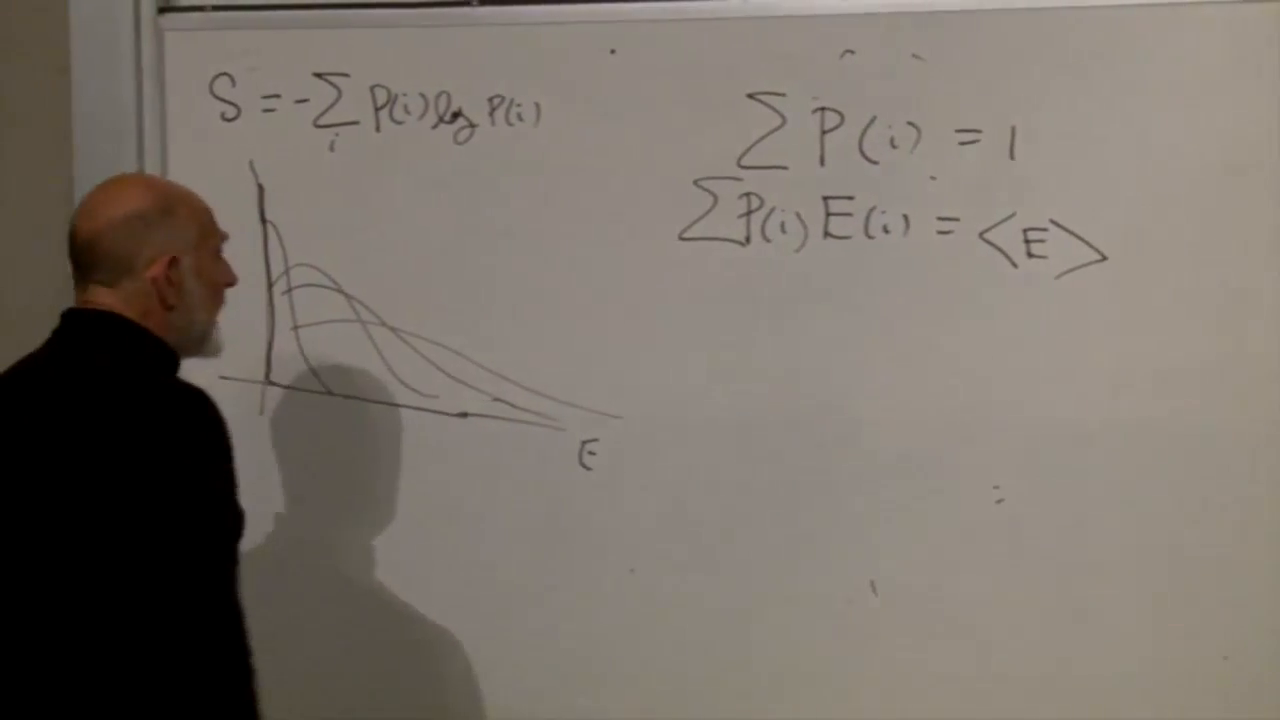
\includegraphics[width=0.88\textwidth]{lecture_03_figure_02.png}
\caption{La pizarra inicial reúne las fórmulas de la entropía, la normalización y la energía media, junto con una familia cualitativa de distribuciones de equilibrio.}
\lectureframe{00:06:44}
\end{figure}

\section{El equilibrio como familia de distribuciones}

La clase anterior nos dejó una familia de distribuciones de equilibrio con un parámetro. Se puede etiquetar esa familia mediante la temperatura, pero por ahora resulta más útil hacerlo mediante la energía media \(\overline E\). A la energía mínima posible, la distribución se concentra en un estado fundamental:
\[
 P_i=\delta_{i0}.
\]
En ese caso no hay incertidumbre sobre el estado y \(S=0\). A medida que la distribución de equilibrio se extiende por más niveles de energía, aumentan tanto su energía media como su entropía.

Esto es cierto para la familia térmica, no para cualquier distribución que se pueda imaginar. Una familia arbitraria podría desplazarse hacia energías mayores y, al mismo tiempo, estrecharse. Las distribuciones de equilibrio que deduciremos no se comportan así en el régimen habitual de temperatura positiva. A lo largo de esa familia,
\begin{equation}
 \frac{dS}{d\overline E}>0.
 \label{eq:sm3-positive-temperature-branch}
\end{equation}
Los sistemas con espectros acotados también pueden tener ramas en las que esta derivada es negativa. Esos regímenes de temperatura negativa son reales, pero los dejaremos de lado en el argumento presente.

El equilibrio térmico es algo más que la inmovilidad microscópica. Las moléculas siguen moviéndose, chocando e intercambiando energía. Lo que se vuelve estacionario es la descripción macroscópica: la distribución deja de presentar una deriva neta y las distintas partes del sistema dejan de mantener un flujo neto de energía.

\section{Las leyes de la termodinámica en lenguaje estadístico}

La primera ley expresa la conservación de la energía. La segunda ley establece que la entropía termodinámica de un sistema macroscópico aislado no disminuye:
\begin{equation}
 \Delta S_{\mathrm{tot}}\geq0.
 \label{eq:sm3-second-law}
\end{equation}
La igualdad describe el equilibrio o un cambio reversible ideal; una relajación espontánea suele producir un aumento estricto.

En el enfoque probabilístico, la relajación tiende a repartir el peso entre las alternativas macroscópicas que aún distinguimos. Esta afirmación requiere la precisión que se hizo en la clase: estamos haciendo un \emph{coarse-graining}. La evolución hamiltoniana exacta conserva la entropía del espacio de fases de grano fino. La entropía macroscópica aumenta porque dejamos de seguir las correlaciones y los detalles microscópicos. Al perder esa información, la descripción reducida se vuelve más amplia. Un estrechamiento espontáneo implicaría, en cambio, que hemos adquirido información microscópica sin realizar una medición.

La ley cero afirma que los sistemas pueden alcanzar el equilibrio térmico y que el equilibrio es transitivo. Si \(A\) está en equilibrio con \(B\), y \(B\) con \(C\), entonces \(A\) está en equilibrio con \(C\). La temperatura proporciona la magnitud que hace explícita esta transitividad:
\[
 T_A=T_B,\qquad T_B=T_C
 \quad\Longrightarrow\quad
 T_A=T_C.
\]
Fuera del equilibrio, la energía fluye del subsistema de mayor temperatura al de menor temperatura. Cuando las temperaturas son iguales, el flujo neto cesa. Ahora deduciremos esta afirmación operacional a partir de la definición de temperatura basada en la entropía.

\section{Por qué la energía fluye de caliente a frío}

Consideremos dos subsistemas débilmente acoplados, \(A\) y \(B\). Cada uno está en equilibrio interno, pero sus temperaturas son distintas. Elijamos las etiquetas de modo que
\begin{equation}
 T_B>T_A>0.
 \label{eq:sm3-temperature-order}
\end{equation}
Durante un pequeño intercambio, la conservación de la energía total da
\begin{equation}
 dE_A+dE_B=0.
 \label{eq:sm3-energy-conservation}
\end{equation}
La segunda ley establece que
\begin{equation}
 dS_A+dS_B\geq0.
 \label{eq:sm3-entropy-change}
\end{equation}
Para cada subsistema en equilibrio interno, la temperatura se define mediante
\begin{equation}
 dE_X=T_X\,dS_X,
 \qquad X=A,B.
 \label{eq:sm3-temperature-differential}
\end{equation}
Al sustituir en \eqref{eq:sm3-energy-conservation} se obtiene
\begin{equation}
 T_A\,dS_A+T_B\,dS_B=0,
\end{equation}
y, por tanto,
\begin{equation}
 dS_B=-\frac{T_A}{T_B}\,dS_A.
 \label{eq:sm3-dsb}
\end{equation}
Al introducir este resultado en \eqref{eq:sm3-entropy-change},
\begin{align}
 dS_{\mathrm{tot}}
 &=dS_A-\frac{T_A}{T_B}dS_A\\
 &=\frac{T_B-T_A}{T_B}\,dS_A\geq0.
 \label{eq:sm3-flow-entropy}
\end{align}
Como \(T_B-T_A>0\) y \(T_B>0\), un intercambio espontáneo requiere que
\[
 dS_A>0.
\]
Entonces, la ecuación \eqref{eq:sm3-temperature-differential} da
\begin{equation}
 dE_A=T_A\,dS_A>0,
 \qquad
 dE_B=-dE_A<0.
 \label{eq:sm3-hot-to-cold}
\end{equation}
La energía ha fluido desde \(B\), el subsistema más caliente, hacia \(A\), el más frío. Aquí, el calor no es más que energía en tránsito. El flujo continúa hasta que \(T_A=T_B\), cuando el cambio de entropía de primer orden deja de favorecer cualquiera de los dos sentidos.

El mismo resultado se puede expresar en una sola línea:
\begin{equation}
 dS_{\mathrm{tot}}
 =dE_A\left(\frac{1}{T_A}-\frac{1}{T_B}\right)\geq0.
 \label{eq:sm3-compact-flow}
\end{equation}
El signo de la diferencia de temperaturas inversas determina el signo de \(dE_A\). Esta forma compacta encajará de manera natural con el conjunto canónico más adelante.

\begin{classroomqa}
\audiencequestion{¿Este argumento supone que \(A\) y \(B\) ya están cada uno en equilibrio interno?}
\lecturerresponse{Sí. Asignar un único \(T_A\) o \(T_B\) implica ese supuesto. Si un subsistema no está en equilibrio interno, hay que dividirlo en regiones más pequeñas y aplicar localmente el argumento allí donde se pueda definir una temperatura. La relajación global se obtiene entonces a partir de los intercambios entre esas regiones.
\lecturetimestamp{00:24:38--00:25:22}}
\end{classroomqa}

\section{¿Qué cuenta como estado?}

Antes de preguntar cuáles son las probabilidades de equilibrio, debemos saber qué significa la etiqueta \(i\). Un estado microscópico es la especificación más completa del sistema que permiten las leyes físicas subyacentes. En mecánica clásica, se imagina que se dan las posiciones y los momentos de todas las partículas. En mecánica cuántica, en cambio, un estado es un estado cuántico completo; el principio de incertidumbre impide especificar simultáneamente con precisión todas las posiciones y momentos clásicos.

Para un sistema cuántico en una caja finita, el recuento pertinente de estados puede ser discreto. La mecánica estadística clásica surge en un límite apropiado, en el que las sumas sobre estados cuánticos muy próximos entre sí se convierten en integrales sobre el espacio de fases. Ese proceso límite también introduce la celda del espacio de fases necesaria para que la entropía continua sea adimensional; no se obtiene simplemente sustituyendo un signo de suma por uno de integral.

\begin{classroomqa}
\audiencequestion{Para un gas, ¿hay que imaginar un estado como las posiciones y los momentos de cada molécula?}
\lecturerresponse{Esa es la imagen clásica correcta. En general, un estado significa todo lo que, en principio, se podría conocer del sistema, de acuerdo con las leyes físicas. La mecánica cuántica modifica la forma de esa descripción máxima y hace discreto el recuento en un volumen finito. Recuperar la integral clásica a partir de la suma cuántica requiere un verdadero argumento de paso al límite, no una sustitución en una sola línea.
\lecturetimestamp{00:25:31--00:27:38}}
\end{classroomqa}

\section{Un baño térmico compuesto de réplicas}

Ahora ya no podemos eludir la pregunta difícil: una vez establecido el equilibrio, ¿qué determina \(P_i\)?

Pongamos el subsistema en contacto con un baño térmico muy grande. La energía puede pasar en ambos sentidos, pero el baño tiene tantos grados de libertad que la transferencia de una pequeña cantidad de energía apenas cambia su temperatura. Un baño especialmente conveniente consiste en muchas réplicas del propio subsistema, débilmente acopladas entre sí. Una réplica es el sistema que estudiamos; las demás constituyen su entorno.

Esta construcción suele reflejar un sistema macroscópico real. Dividamos un cuerpo grande y casi homogéneo en muchas celdas similares. Cada celda es un subsistema y las celdas restantes actúan como su baño. Denotemos por \(N\) el número total de réplicas. La demostración en clase usa nueve réplicas y tres etiquetas de estado de distintos colores, pero el recuento no depende de esos números concretos.

Sea \(n_i\) el número de réplicas en el estado \(i\). Estos son los \emph{números de ocupación}. Puede haber infinitos niveles de energía posibles, pero, a energía total finita, la ocupación de la mayoría de los niveles muy altos es despreciable o nula.

La primera restricción expresa simplemente el número de réplicas:
\begin{equation}
 \sum_i n_i=N.
 \label{eq:sm3-number-constraint}
\end{equation}
La segunda es la energía total:
\begin{equation}
 \sum_i n_iE_i=N\overline E.
 \label{eq:sm3-total-energy-constraint}
\end{equation}
El miembro derecho es extensivo. Si se duplica el número de réplicas manteniendo fijo su estado estadístico, se duplica la energía total, mientras que la energía media por réplica sigue siendo \(\overline E\).

\begin{classroomqa}
\audiencequestion{¿La construcción con réplicas también debe satisfacer una restricción de energía?}
\lecturerresponse{Sí. Los números de ocupación deben sumar \(N\), y su suma ponderada por la energía debe ser igual a la energía total fija \(N\overline E\). Esas son precisamente las dos restricciones que limitarán más adelante la maximización de la entropía.
\lecturetimestamp{00:37:12--00:39:54}}
\end{classroomqa}

La probabilidad de que una réplica elegida al azar ocupe el estado \(i\) es su frecuencia relativa:
\begin{equation}
 P_i=\frac{n_i}{N},
 \qquad
 n_i=NP_i.
 \label{eq:sm3-frequency-probability}
\end{equation}

\begin{figure}[t]
\centering
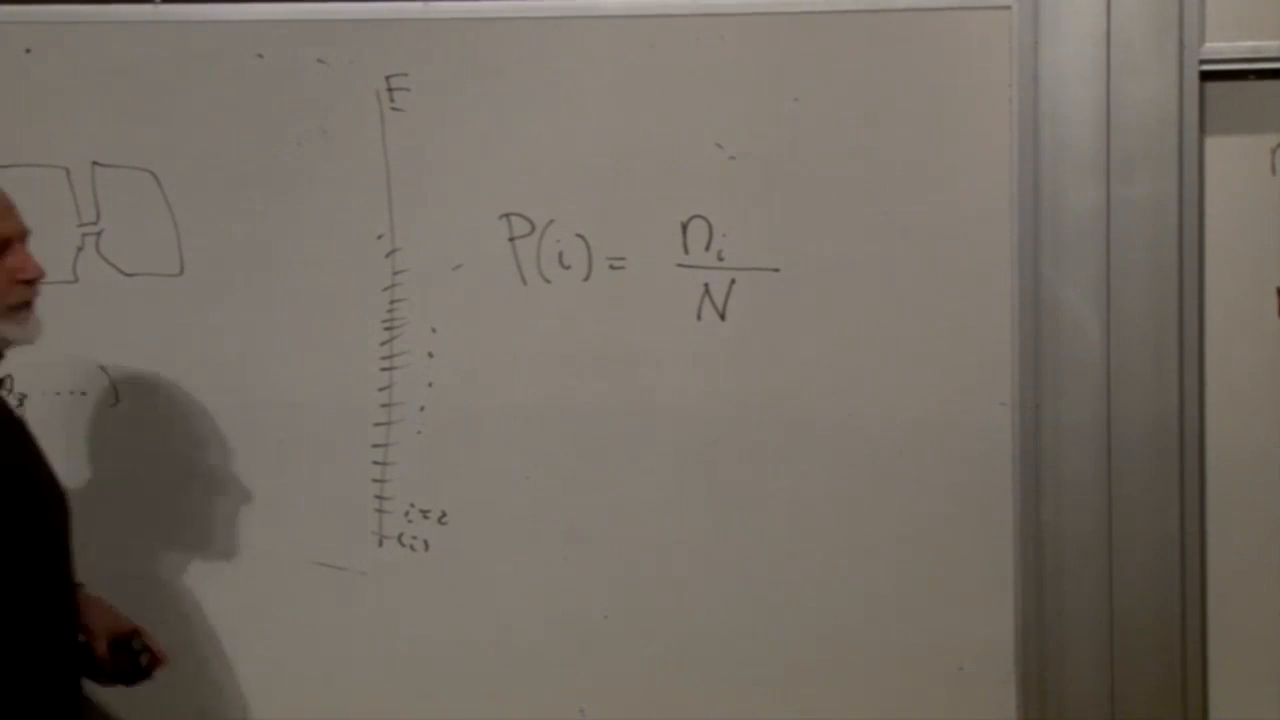
\includegraphics[width=0.82\textwidth]{lecture_03_figure_03.png}
\caption{La imagen de los niveles de energía y la identificación de la probabilidad con la fracción de ocupación \(P_i=n_i/N\).}
\lectureframe{00:41:40}
\end{figure}

\begin{classroomqa}
\audiencequestion{¿Se pretende que la notación \(N(i)\) de la pizarra sea distinta de \(n_i\)?}
\lecturerresponse{No. Ambas notaciones representan el número de ocupación del estado \(i\). Usaremos \(n_i\) de manera sistemática y reservaremos la mayúscula \(N\) para el número total de réplicas.
\lecturetimestamp{00:41:28--00:41:33}}
\end{classroomqa}

Al dividir \eqref{eq:sm3-number-constraint} y \eqref{eq:sm3-total-energy-constraint} entre \(N\) se recuperan las restricciones sobre las probabilidades:
\begin{equation}
 \sum_iP_i=1,
 \qquad
 \sum_iP_iE_i=\overline E.
 \label{eq:sm3-probability-constraints}
\end{equation}
La interpretación de las frecuencias en el conjunto ha reproducido, por tanto, las ecuaciones con las que empezamos.

\section{Multiplicidad de un patrón de ocupación}

Fijemos un conjunto de números de ocupación \(\{n_i\}\). ¿Cuántas asignaciones de las \(N\) réplicas distinguibles a los estados dan exactamente ese conjunto? La respuesta es el coeficiente multinomial
\begin{equation}
 C(\{n_i\})=\frac{N!}{\prod_i n_i!}.
 \label{eq:sm3-multiplicity}
\end{equation}
Para entender el denominador, primero ordenamos las \(N\) réplicas etiquetadas de \(N!\) maneras. Reordenar las \(n_i\) réplicas que ocupan el mismo estado no genera una nueva asignación de ocupación, así que dividimos por \(n_i!\) para cada estado.

\begin{figure}[t]
\centering
\includegraphics[width=0.88\textwidth]{lecture_03_figure_04.png}
\caption{La multiplicidad multinomial \(C=N!/\prod_i n_i!\) escrita en la pizarra.}
\lectureframe{00:46:55}
\end{figure}

Los niveles desocupados no plantean ningún problema porque \(0!=1\). Si todas las réplicas ocupan un mismo estado, entonces
\[
 C=\frac{N!}{N!}=1,
\]
como cabía esperar. Si tres réplicas ocupan tres estados especificados distintos, entonces
\[
 C=\frac{3!}{1!\,1!\,1!}=6.
\]
Cuando dos réplicas ocupan dos estados especificados, la fórmula da dos asignaciones: se intercambia cuál de las réplicas etiquetadas ocupa cada estado.

\begin{classroomqa}
\audiencequestion{¿Puede haber más de un conjunto de números de ocupación que satisfaga las dos restricciones?}
\lecturerresponse{Por lo general, sí, hay muchos. La ecuación \eqref{eq:sm3-multiplicity} cuenta primero las configuraciones para un conjunto fijo \(\{n_i\}\), sin decidir aún si satisface las restricciones. En la etapa siguiente se comparan todos los conjuntos compatibles con ellas y se encuentra cuál tiene la multiplicidad más grande.
\lecturetimestamp{00:48:07--00:48:43}}
\end{classroomqa}

El supuesto estadístico es que las asignaciones microscópicas compatibles con la configuración aislada se tratan simétricamente. Por tanto, un patrón macroscópico de ocupación que se realiza de más maneras es más probable. Cuando \(N\) es grande, la distribución de las fracciones \(n_i/N\) tiene un pico muy pronunciado. Las fracciones de equilibrio son los valores que maximizan \(C\), con las restricciones \eqref{eq:sm3-number-constraint} y \eqref{eq:sm3-total-energy-constraint}.

\section{La aproximación de Stirling}

Los factoriales se vuelven enormes mucho antes de que \(N\) alcance un valor macroscópico, así que trabajamos con sus logaritmos. Empecemos por
\begin{equation}
 \log N!=\sum_{x=1}^{N}\log x.
 \label{eq:sm3-log-factorial-sum}
\end{equation}
Para valores grandes de \(N\), la suma se aproxima mediante el área bajo \(\log x\):
\begin{align}
 \log N!
 &\simeq\int_1^N\log x\,dx\\
 &=\left[x\log x-x\right]_1^N\\
 &=N\log N-N+1.
 \label{eq:sm3-stirling-integral}
\end{align}
La primitiva se obtiene directamente de
\[
 \frac{d}{dx}(x\log x-x)=\log x.
\]
En el orden extensivo dominante, se puede omitir la constante aditiva:
\begin{equation}
 \log N!\simeq N\log N-N.
 \label{eq:sm3-stirling-log}
\end{equation}
Al exponenciar se obtiene la forma simplificada que se usa en la clase,
\begin{equation}
 N!\simeq N^N e^{-N}.
 \label{eq:sm3-stirling-simple}
\end{equation}

\begin{figure}[t]
\centering
\includegraphics[width=0.88\textwidth]{lecture_03_figure_05.png}
\caption{La aproximación de Stirling dominante y su deducción al sustituir la suma de \(\log x\) por una integral.}
\lectureframe{01:03:45}
\end{figure}

\begin{classroomqa}
\audiencequestion{Al evaluar \(x\log x-x\) en el límite inferior, ¿queda un \(+1\) adicional?}
\lecturerresponse{Sí. La ecuación \eqref{eq:sm3-stirling-integral} contiene esa constante. Es despreciable frente a los términos proporcionales a \(N\) cuando \(N\to\infty\), por lo que la fórmula dominante la omite. La suma debe empezar en \(x=1\); \(\log0\) no está definido.
\lecturetimestamp{01:04:12--01:04:35}}
\end{classroomqa}

\begin{classroomqa}
\audiencequestion{¿Falta también un factor proporcional a \(\sqrt{N}\)?}
\lecturerresponse{Sí. La fórmula asintótica más precisa es
\[
 N!\sim\sqrt{2\pi N}\left(\frac{N}{e}\right)^N.
\]
Su logaritmo añade solo \(\tfrac12\log(2\pi N)\), que es subextensivo en comparación con \(N\log N-N\). Es relevante para calcular con precisión probabilidades a \(N\) finito, pero no para el cálculo dominante de la entropía de un sistema macroscópico.
\lecturetimestamp{01:04:35--01:05:40}}
\end{classroomqa}

La aproximación de Stirling también debe aplicarse con cuidado al denominador de \eqref{eq:sm3-multiplicity}. En el límite termodinámico, los estados con probabilidades límite no nulas satisfacen \(n_i=NP_i\), de modo que sus ocupaciones crecen con \(N\). Los estados con ocupación muy pequeña o nula se pueden tratar mediante un corte de energía finito y reincorporar después tomando un límite. Los términos subdominantes omitidos no afectan a la entropía extensiva dominante.

\section{El logaritmo de la multiplicidad es la entropía}

Apliquemos \eqref{eq:sm3-stirling-simple} al numerador y a todos los factores del denominador con ocupación macroscópica:
\begin{equation}
 C\simeq
 \frac{N^Ne^{-N}}
 {\prod_i n_i^{\,n_i}e^{-n_i}}.
 \label{eq:sm3-c-stirling}
\end{equation}
Como \(\sum_i n_i=N\), los factores exponenciales dominantes se cancelan:
\begin{equation}
 C\simeq\frac{N^N}{\prod_i n_i^{\,n_i}}.
 \label{eq:sm3-c-leading}
\end{equation}
Es más fácil maximizar un logaritmo que un producto y, como el logaritmo es monótono, ambas funciones alcanzan el máximo con el mismo patrón de ocupación:
\begin{equation}
 \log C=N\log N-\sum_i n_i\log n_i.
 \label{eq:sm3-logc-occupations}
\end{equation}
Ahora sustituimos \(n_i=NP_i\):
\begin{align}
 \log C
 &=N\log N-\sum_iNP_i\log(NP_i)\\
 &=N\log N-N\sum_iP_i\log N
   -N\sum_iP_i\log P_i\\
 &=-N\sum_iP_i\log P_i,
 \label{eq:sm3-logc-entropy-derivation}
\end{align}
donde la normalización cancela los dos términos \(N\log N\). Así, en el orden dominante en \(N\),
\begin{equation}
 \boxed{\log C=NS}.
 \label{eq:sm3-logc-ns}
\end{equation}

\begin{figure}[t]
\centering
\includegraphics[width=0.88\textwidth]{lecture_03_figure_06.png}
\caption{El cálculo en la pizarra que relaciona \(\log C=N\log N-\sum_i n_i\log n_i\) con \(-N\sum_iP_i\log P_i=NS\).}
\lectureframe{01:16:10}
\end{figure}

Esta relación es el núcleo conceptual del capítulo. La entropía no es una magnitud ajena que se imponga al problema de recuento. Es la multiplicidad por réplica, expresada mediante un logaritmo. Por tanto, maximizar el número de configuraciones microscópicas equivale, en el orden dominante, a maximizar la entropía de una réplica.

\begin{classroomqa}
\audiencequestion{¿No sería máxima la multiplicidad si todos los números de ocupación fueran iguales?}
\lecturerresponse{La distribución es uniforme cuando ningún estado está destacado y solo se impone \(\sum_i n_i=N\) en un conjunto finito de estados. La restricción de energía fija cambia el resultado porque los valores \(E_i\) son distintos. En general, las ocupaciones iguales no producen la energía media especificada.
\lecturetimestamp{01:17:07--01:18:20}}
\end{classroomqa}

\begin{classroomqa}
\audiencequestion{La mayúscula \(N\) es grande, pero ¿por qué se puede aplicar la aproximación de Stirling a cada \(n_i\) del denominador?}
\lecturerresponse{Para cada estado con probabilidad límite no nula, \(n_i=NP_i\) crece proporcionalmente a \(N\). Primero se puede conservar un intervalo finito de energías, tomar allí el límite de \(N\) grande y, después, ampliar el intervalo. Los estados dispersos de la cola requieren correcciones finitas por separado, pero no alteran la entropía extensiva dominante.
\lecturetimestamp{01:18:23--01:19:28}}
\end{classroomqa}

\begin{classroomqa}
\audiencequestion{¿Esta aproximación para \(N\) grande es lo que antes se llamaba coarse-graining?}
\lecturerresponse{No. El límite termodinámico controla los grandes números de ocupación y el recuento asintótico. El coarse-graining consiste en perder o descartar deliberadamente la resolución microscópica. Son operaciones distintas, aunque ambas se usan a menudo en la mecánica estadística macroscópica.
\lecturetimestamp{01:19:29--01:19:46}}
\end{classroomqa}

\begin{classroomqa}
\audiencequestion{Como \(\log C=N\log N-\sum_i n_i\log n_i\), ¿no habría que minimizar el segundo término en vez de maximizarlo?}
\lecturerresponse{Sí; con \(N\) fijo, maximizar \(\log C\) equivale a minimizar \(\sum_i n_i\log n_i\). Después de sustituir \(n_i=NP_i\), se cancelan los términos fijos \(N\log N\) y queda \(-N\sum_iP_i\log P_i=NS\). Por eso, resulta más natural describir la misma operación como la maximización de la entropía positiva \(S\).
\lecturetimestamp{01:19:48--01:20:55}}
\end{classroomqa}

\begin{classroomqa}
\audiencequestion{¿Por qué no terminar enseguida el argumento por simetría e igualar todos los \(n_i\)?}
\lecturerresponse{Ese atajo pasa por alto las etiquetas de energía. La restricción de normalización trata los estados simétricamente, pero \(\sum_iP_iE_i=\overline E\) no lo hace: los estados con energías distintas contribuyen de manera diferente. La restricción de energía es precisamente donde entra la distribución de equilibrio no uniforme.
\lecturetimestamp{01:21:15--01:21:41}}
\end{classroomqa}

\section{El problema de maximización de la entropía}

Ahora podemos enunciar sin ambigüedad la regla de la mecánica estadística. Variamos las probabilidades \(P_i\) y maximizamos
\begin{equation}
 S[P]=-\sum_iP_i\log P_i
 \label{eq:sm3-maximize-entropy}
\end{equation}
sujeto a
\begin{equation}
 \sum_iP_i=1,
 \qquad
 \sum_iP_iE_i=\overline E.
 \label{eq:sm3-maxent-constraints}
\end{equation}
Las probabilidades que maximizan la entropía dan las fracciones de ocupación marcadamente preferidas en un conjunto grande de réplicas. Los números de ocupación fluctúan, pero sus desviaciones relativas disminuyen a medida que crece \(N\), de modo que las razones \(n_i/N\) quedan bien definidas como probabilidades termodinámicas.

\begin{classroomqa}
\audiencequestion{¿Las energías de estado \(E_i\) están fijas, mientras que la restricción usa una energía total dada por separado?}
\lecturerresponse{Sí. El espectro \(\{E_i\}\) pertenece al subsistema. La colección completa de réplicas tiene una energía total fija, pero la energía se intercambia continuamente entre las réplicas. Dividir ese total entre \(N\) fija la energía media \(\overline E\) de una réplica, no su energía en cada realización microscópica.
\lecturetimestamp{01:26:12--01:27:07}}
\end{classroomqa}

El problema es fácil de enunciar, pero todavía no está resuelto. Se trata de una extremización con dos restricciones, así que hace falta una herramienta matemática más.

\section{Multiplicadores de Lagrange}

Para una función no restringida \(F(x_1,x_2,\ldots)\), un punto estacionario satisface
\begin{equation}
 \frac{\partial F}{\partial x_i}=0
 \qquad\text{for every }i.
 \label{eq:sm3-unconstrained-stationary}
\end{equation}
Supongamos ahora, además, que exigimos
\begin{equation}
 G(x_1,x_2,\ldots)=0.
 \label{eq:sm3-one-constraint}
\end{equation}

\begin{classroomqa}
\audiencequestion{En el diagrama, ¿qué significa \(x\) si las coordenadas son \(x\) y \(y\)?}
\lecturerresponse{Aquí \(x\) es una abreviatura del vector de coordenadas completo \((x_1,x_2,\ldots)\). En el dibujo bidimensional, sus componentes son sencillamente \(x\) y \(y\). Más adelante, las componentes serán las probabilidades \(P_1,P_2,\ldots\).
\lecturetimestamp{01:30:12--01:30:20}}
\end{classroomqa}

Desde el punto de vista geométrico, las curvas de nivel \(F=\text{constant}\) forman un mapa de contornos, mientras que \(G=0\) es la curva sobre la que el sistema puede moverse. Un extremo con restricciones se alcanza cuando una curva de nivel de \(F\) es tangente a la curva de restricción. En ese punto, los gradientes son paralelos:
\begin{equation}
 \nabla F=-\lambda\nabla G
 \label{eq:sm3-parallel-gradients}
\end{equation}
para algún número \(\lambda\).

\begin{figure}[t]
\centering
\includegraphics[width=0.88\textwidth]{lecture_03_figure_07.png}
\caption{La geometría de contornos de la pizarra y la función aumentada \(F'=F+\lambda G\). El extremo con restricciones se alcanza en el punto de tangencia.}
\lectureframe{01:37:10}
\end{figure}

La ecuación \eqref{eq:sm3-parallel-gradients} se obtiene definiendo la función aumentada
\begin{equation}
 F'=F+\lambda G
 \label{eq:sm3-augmented-function}
\end{equation}
y exigiendo la condición habitual de estacionariedad:
\begin{equation}
 \frac{\partial F'}{\partial x_i}=0.
 \label{eq:sm3-augmented-stationarity}
\end{equation}
El multiplicador \(\lambda\) es desconocido al principio. Esto no deja el sistema indeterminado, porque la restricción original \(G=0\) aporta una ecuación adicional.

\begin{classroomqa}
\classquestion{¿Por qué añadir un término proporcional a \(G\) hace que el punto con restricciones sea estacionario?}
\lecturerresponse{En el extremo con restricciones, el movimiento tangente a \(G=0\) ya no produce un cambio de primer orden en \(F\). La única pendiente que queda es normal a la restricción. Como \(\nabla G\) apunta en esa misma dirección normal, un valor adecuado de \(\lambda\) la cancela:
\(\nabla F+\lambda\nabla G=0\).
\lecturetimestamp{01:35:06--01:35:32}}
\end{classroomqa}

\section{Un ejemplo con dos variables}

Minimicemos
\begin{equation}
 F(x,y)=\frac{x^2+y^2}{2}
 \label{eq:sm3-example-f}
\end{equation}
sujeto a
\begin{equation}
 x+y=1.
 \label{eq:sm3-example-constraint}
\end{equation}
Escribamos la restricción como \(G=x+y-1=0\) y formemos
\begin{equation}
 F'=\frac{x^2+y^2}{2}+\lambda(x+y-1).
 \label{eq:sm3-example-augmented}
\end{equation}
Las ecuaciones de estacionariedad son
\begin{align}
 \frac{\partial F'}{\partial x}&=x+\lambda=0,\\
 \frac{\partial F'}{\partial y}&=y+\lambda=0.
 \label{eq:sm3-example-derivatives}
\end{align}
Así, \(x=y=-\lambda\). La ecuación restante es la restricción,
\[
 x+y=-2\lambda=1,
\]
por lo que
\begin{equation}
 \lambda=-\frac12,
 \qquad
 x=y=\frac12.
 \label{eq:sm3-example-solution}
\end{equation}
El punto \((1/2,1/2)\) es donde la circunferencia más pequeña centrada en el origen toca la recta \(x+y=1\).

\begin{figure}[t]
\centering
\includegraphics[width=0.88\textwidth]{lecture_03_figure_08.png}
\caption{El cálculo completo con multiplicadores de Lagrange para minimizar \((x^2+y^2)/2\) sujeto a \(x+y=1\).}
\lectureframe{01:44:10}
\end{figure}

Con varias restricciones, se introduce un multiplicador por cada una:
\begin{equation}
 F'=F+\lambda_1G_1+\lambda_2G_2+\cdots.
 \label{eq:sm3-many-multipliers}
\end{equation}
Después se resuelve
\begin{equation}
 \begin{aligned}
 \frac{\partial F'}{\partial x_i}&=0
 &&\text{for every }i,\\
 G_a&=0
 &&\text{for every constraint }a.
 \end{aligned}
 \label{eq:sm3-many-equations}
\end{equation}
La clase propone un ejercicio de práctica deliberadamente artificial: extremar una función cuadrática de \(x,y,z\) imponiendo dos restricciones lineales independientes, por ejemplo \(x+y=1\) y \(z+x=1\). El objetivo no es obtener una respuesta concreta, sino aprender la regla: cada restricción aporta un multiplicador y una ecuación.

\section{El problema queda planteado para la próxima clase}

En mecánica estadística, las coordenadas son las probabilidades \(\{P_i\}\), la función que se maximiza es la entropía y las restricciones son la normalización y una energía media fija. Definamos
\begin{align}
 S[P]&=-\sum_iP_i\log P_i,\\
 G_1[P]&=\sum_iP_i-1,\\
 G_2[P]&=\sum_iP_iE_i-\overline E.
 \label{eq:sm3-final-functions}
\end{align}
Por tanto, la entropía aumentada se puede escribir como
\begin{equation}
 \Phi[P]
 =S[P]+\alpha G_1[P]+\beta G_2[P].
 \label{eq:sm3-final-augmented}
\end{equation}
Las ecuaciones que hay que resolver son
\begin{equation}
 \frac{\partial\Phi}{\partial P_i}=0
 \quad\text{for every }i,
 \qquad
 G_1=0,
 \qquad
 G_2=0.
 \label{eq:sm3-final-problem}
\end{equation}

\begin{figure}[H]
\centering
\includegraphics[width=0.88\textwidth]{lecture_03_figure_09.png}
\caption{La pizarra final: la entropía como función de las probabilidades, junto con la normalización y la energía media fija.}
\lectureframe{01:53:05}
\end{figure}

En este punto el problema está completamente planteado. Resolver \eqref{eq:sm3-final-problem} produce la distribución de equilibrio. El multiplicador conjugado a la energía se convertirá en la temperatura inversa \(\beta=1/T\), según la convención de signos elegida en \eqref{eq:sm3-final-augmented}. En la próxima clase se llevará a cabo esa derivación y se obtendrán los pesos de Boltzmann.
\chapter{Pesos de Boltzmann, funciones de partición y gas ideal}

\lectureoverview{Derivamos la distribución de probabilidad de equilibrio maximizando la entropía con la normalización y la energía media fijas. La función de partición permite obtener después la energía media, la entropía y la temperatura mediante derivación. El gas ideal proporciona el primer ejemplo completo; a continuación se presenta una extensión gravitatoria y un anticipo de las fluctuaciones de energía.}

\section{El problema de maximizar la entropía con restricciones}

Partamos de una gran colección de \(\mathcal N\) réplicas idénticas de un mismo subsistema que interactúan muy débilmente entre sí. Si \(n_i\) réplicas ocupan el estado \(i\)-ésimo, entonces
\begin{equation}
 p_i=\frac{n_i}{\mathcal N},
 \qquad
 \sum_i p_i=1.
 \label{eq:sm4-occupation-probability}
\end{equation}
El recuento multinomial de la clase anterior da la entropía por réplica:
\begin{equation}
 S[p]=-\sum_i p_i\log p_i.
 \label{eq:sm4-entropy}
\end{equation}
Conviene verla como una función ordinaria de todas las variables \(p_1,p_2,\ldots\). Su sencilla forma aditiva es lo que hace posible el cálculo.

La colección de réplicas tiene una energía total fija \(\mathcal N E\), donde \(E\) es la energía media por réplica. La segunda restricción es, por tanto,
\begin{equation}
 \sum_i p_iE_i=E.
 \label{eq:sm4-energy-constraint}
\end{equation}
Los niveles \(E_i\) pertenecen al subsistema; el número \(E\) del lado derecho es su promedio ponderado por las probabilidades. Maximizar \eqref{eq:sm4-entropy} sujeto a \eqref{eq:sm4-occupation-probability} y \eqref{eq:sm4-energy-constraint} selecciona las fracciones de ocupación abrumadoramente más probables.

Para mayor comodidad, minimicemos \(-S=\sum_i p_i\log p_i\). Introduzcamos un multiplicador de Lagrange por cada restricción:
\begin{equation}
 \begin{aligned}
 \Phi[p;\alpha,\beta]
 &=\sum_i p_i\log p_i\\
 &\quad+\alpha\left(\sum_i p_i-1\right)\\
 &\quad+\beta\left(\sum_i p_iE_i-E\right).
 \end{aligned}
 \label{eq:sm4-augmented-functional}
\end{equation}
Los nombres \(\alpha\) y \(\beta\) todavía no representan supuestos físicos. En esta etapa son simplemente los dos números necesarios para imponer las dos restricciones.

\begin{classroomqa}\audiencequestion{¿La función ampliada también depende de \(\alpha\) y \(\beta\)?}\lecturerresponse{Sí. Al variarla con respecto a \(\alpha\) y \(\beta\) se recuperan las dos restricciones. Sin embargo, para el cálculo inmediato mantenemos fijos esos multiplicadores y variamos las probabilidades \(p_i\). Sus valores quedan determinados después por la normalización y la energía media prescrita.
\lecturetimestamp{00:09:32--00:09:49}}\end{classroomqa}

\begin{figure}[t]\centering
\includegraphics[width=0.92\textwidth]{lecture_04_figure_02.png}\caption{Funcional de entropía ampliado, tras omitir los términos constantes al variar las probabilidades.}\lectureframe{00:10:56}\end{figure}

Al derivar con respecto a una probabilidad, los términos \(-\alpha\) y \(-\beta E\) no contribuyen. Este es el funcional abreviado que aparece en la pizarra. Siguen formando parte de \eqref{eq:sm4-augmented-functional}; simplemente han dejado de importar para esta derivada concreta.

\section{La distribución de Boltzmann}

Elijamos cualquier probabilidad. En la clase se elige \(p_7\), en parte porque \(1\) parece demasiado especial y \(7\) trae suerte. La elección no afecta al resultado. Solo hace falta usar esta derivada:
\begin{equation}
 \frac{d}{dp_i}\bigl(p_i\log p_i\bigr)=\log p_i+1.
\end{equation}
Así que
\begin{equation}
 \frac{\partial\Phi}{\partial p_i}
 =\log p_i+1+\alpha+\beta E_i=0.
 \label{eq:sm4-stationarity}
\end{equation}
Despejando \(p_i\),
\begin{align}
 \log p_i&=-(1+\alpha)-\beta E_i,\\
 p_i&=e^{-(1+\alpha)}e^{-\beta E_i}.
\end{align}
El primer factor no depende del índice del estado. Escribámoslo como \(1/Z\):
\begin{equation}
 p_i=\frac{e^{-\beta E_i}}{Z}.
 \label{eq:sm4-boltzmann-weight}
\end{equation}

Este es el primer resultado inesperado. Una derivada rutinaria con restricciones ha producido una ley exponencial. Las probabilidades relativas obedecen
\begin{equation}
 \frac{p_i}{p_j}=e^{-\beta(E_i-E_j)}.
 \label{eq:sm4-relative-weight}
\end{equation}
El multiplicador \(\beta\) controla la rapidez con que la probabilidad disminuye al aumentar la energía. Un valor grande y positivo de \(\beta\) concentra la distribución cerca de los niveles más bajos; un valor pequeño y positivo de \(\beta\) reparte un peso apreciable entre niveles más altos del espectro. Ya podemos ver que cambiar \(\beta\) modifica la energía media, aunque todavía hay que demostrar que corresponde a la inversa de la temperatura.

\section{Normalización y función de partición}

La normalización determina el factor independiente del estado:
\begin{equation}
 1=\sum_i p_i
 =\frac{1}{Z}\sum_i e^{-\beta E_i},
\end{equation}
por tanto,
\begin{equation}
 Z(\beta)=\sum_i e^{-\beta E_i}.
 \label{eq:sm4-partition-function}
\end{equation}
Esta es la función de partición canónica. Apareció primero como una constante de normalización, pero esa descripción no refleja en absoluto la importancia de su papel. Una vez conocida \(Z(\beta)\), las derivadas permiten obtener las magnitudes termodinámicas.

Los niveles de energía en \eqref{eq:sm4-partition-function} son datos de entrada. Provienen de la mecánica del sistema y de las condiciones externas fijas: el volumen y la forma de la caja, los campos magnéticos o eléctricos y cualquier otro parámetro de control. Al cambiar un parámetro de control, cambia el espectro y, por tanto, \(Z\). En el cálculo actual, esos parámetros y, en consecuencia, el conjunto \(\{E_i\}\) se mantienen fijos.

\begin{classroomqa}\audiencequestion{¿Qué representan exactamente los ejes del esquema exponencial? ¿La coordenada vertical es un \(p_i\) concreto?}\lecturerresponse{La altura representada es la probabilidad asignada a un nivel; el orden horizontal puede leerse como el índice del estado \(i\) o, de manera más física, como la energía \(E_i\). Cada estado tiene una energía fija. Un valor grande de \(\beta\) hace que la probabilidad disminuya rápidamente al aumentar la energía; cuando \(\beta=0\), los pesos son casi uniformes entre los niveles accesibles.
\lecturetimestamp{00:19:39--00:20:09}}\end{classroomqa}

\section{La energía media oculta en la función de partición}

La segunda restricción determina \(\beta\):
\begin{equation}
 E=\sum_i p_iE_i
 =\frac{1}{Z}\sum_i E_i e^{-\beta E_i}.
 \label{eq:sm4-mean-energy}
\end{equation}
En lugar de volver a calcular esta suma ponderada, derivemos \eqref{eq:sm4-partition-function}:
\begin{equation}
 \frac{dZ}{d\beta}
 =-\sum_i E_i e^{-\beta E_i}.
\end{equation}
Al comparar con \eqref{eq:sm4-mean-energy}, obtenemos
\begin{equation}
 E(\beta)
 =-\frac{1}{Z}\frac{dZ}{d\beta}
 =-\frac{d\log Z}{d\beta}.
 \label{eq:sm4-energy-logz}
\end{equation}
El logaritmo es natural porque su derivada aporta el factor \(1/Z\).

\begin{figure}[t]\centering
\includegraphics[width=0.82\textwidth]{lecture_04_figure_03.png}\caption{La normalización, la restricción sobre la energía media y la derivada de la función de partición aparecen juntas en la pizarra.}\lectureframe{00:26:24}\end{figure}

\begin{classroomqa}\audiencequestion{¿La ecuación inferior de la pizarra es una ecuación nueva para \(Z\) o se obtiene de la definición que aparece encima?}\lecturerresponse{Se obtiene derivando la definición \(Z=\sum_i e^{-\beta E_i}\). La derivada introduce el factor \(-E_i\). Al dividir el resultado por \(Z\), se recupera la suma ponderada que define la energía media.
\lecturetimestamp{00:25:58--00:26:37}}\end{classroomqa}

\begin{classroomqa}\audiencequestion{¿Hace que \(dZ/d\beta=-E Z\) sea una función propia de la derivación?\(Z\)}\lecturerresponse{No en el sentido habitual. Una ecuación de valores propios tendría una constante multiplicando a \(Z\), mientras que aquí \(E=E(\beta)\). La ecuación nos da la energía media en función de \(\beta\); no es un problema de valores propios fijos.
\lecturetimestamp{00:28:49--00:29:43}}\end{classroomqa}

La sencillez de \eqref{eq:sm4-energy-logz} resulta engañosa. El espectro puede ser complicado y calcular \(Z\) puede ser difícil, pero, una vez hallada esa única función, basta una derivada para obtener la energía media. Este patrón se repite en toda la mecánica estadística: las operaciones elementales, aplicadas en el orden adecuado, dan resultados que habría sido difícil adivinar directamente.

\begin{classroomqa}\audiencequestion{¿Es \(E\) la energía total de todas las réplicas o la energía media por caja?}\lecturerresponse{Es la energía media de una caja. La colección de réplicas tiene una energía total \(\mathcal N E\). Más adelante, cuando el sistema elegido sea una caja completa con \(N\) partículas de gas, \(E\) representará la energía de toda esa muestra de gas.
\lecturetimestamp{00:30:55--00:31:10}}\end{classroomqa}

\begin{classroomqa}\audiencequestion{¿Podemos tomar el logaritmo de \(\sum_i e^{-\beta E_i}\) término a término?}\lecturerresponse{No. El logaritmo convierte un producto en una suma, pero no convierte una suma en una suma de logaritmos:
\[
 \log\!\left(\sum_i e^{-\beta E_i}\right)
 \ne \sum_i\log\!\left(e^{-\beta E_i}\right).
\]
Esta distinción será útil más adelante, cuando las funciones de partición de subsistemas independientes se multipliquen.
\lecturetimestamp{00:31:10--00:31:58}}\end{classroomqa}

\section{¿Qué se mantiene fijo y qué puede variar?}

En estas mismas fórmulas aparecen varias capas de variables, y en la discusión en clase se distinguen deliberadamente.

\begin{itemize}\item Las probabilidades \(p_i\) son las incógnitas originales.
 \item Los niveles \(E_i\) quedan fijos una vez especificados el sistema y sus parámetros de control.
 \item El multiplicador \(\alpha\) se ha incorporado a la normalización \(Z=e^{1+\alpha}\).
 \item Para una energía media prescrita \(E\), la restricción fija un valor de \(\beta\). Sin embargo, a lo largo de una familia de estados de equilibrio, puede usarse \(E=E(\beta)\) o \(\beta=\beta(E)\).
\end{itemize}

\begin{classroomqa}\audiencequestion{Si los multiplicadores son números, ¿por qué ahora se trata \(\beta\) y \(E\) como variables?}\lecturerresponse{Para un problema con restricciones son, efectivamente, números. Pero podemos comparar muchos problemas de equilibrio con el mismo espectro y distintas energías medias prescritas. En esa familia, \(\beta\) varía con \(E\). Fijar \(E\) determina \(\beta\); fijar \(\beta\) determina \(E\). Son dos maneras de interpretar la misma relación.
\lecturetimestamp{00:31:58--00:33:27}}\end{classroomqa}

\begin{classroomqa}\audiencequestion{¿Ha desaparecido \(\alpha\)?}\lecturerresponse{Solo ha desaparecido su nombre. La definición \(e^{-(1+\alpha)}=1/Z\) lo incorpora a \(Z\). Mantener tanto \(\alpha\) como \(Z\) sería contar dos veces el mismo parámetro de normalización.
\lecturetimestamp{00:33:29--00:33:49}}\end{classroomqa}

La energía no es la única magnitud conservada posible. Si se impone una restricción sobre el momento total, el número de partículas, el momento angular u otra magnitud, su valor esperado recibe su propio multiplicador. Esta ampliación cambia el conjunto estadístico, pero no el método.

\begin{classroomqa}\audiencequestion{¿Presuponer que basta con fijar la energía media es asumir demasiado sobre el sistema?}\lecturerresponse{Presupone que, en el problema actual, no hace falta condicionar sobre ninguna otra magnitud conservada. Si, por ejemplo, también se fija el momento total, se añade otra restricción y otro multiplicador de Lagrange. En cambio, aquí el volumen, la forma y los campos externos son parámetros de control: se mantienen fijos y determinan los propios niveles de energía.
\lecturetimestamp{00:33:51--00:35:50}}\end{classroomqa}

\begin{classroomqa}\audiencequestion{¿Debería aparecer \(\alpha\) como otro argumento de la energía? ¿Y depende \(Z\) de los niveles \(E_i\)?}\lecturerresponse{\(\alpha\) ya está incluido en \(Z\), así que no es un argumento independiente. La función de partición sí depende tanto del espectro fijo como de \(\beta\). Cambiar un parámetro de control modifica \(E_i\) y, por tanto, \(Z\); durante las derivadas actuales con respecto a \(\beta\), el espectro se mantiene fijo.
\lecturetimestamp{00:35:52--00:37:10}}\end{classroomqa}

\begin{classroomqa}\audiencequestion{¿Estamos variando los niveles individuales \(E_i\) o la energía media \(E\)?}\lecturerresponse{Los niveles individuales permanecen fijos. La energía media cambia porque cambian las probabilidades. Así, la familia se parametriza mediante \(E\) o, de manera equivalente, mediante \(\beta\), mientras que se mantiene la misma lista de niveles \(\{E_i\}\).
\lecturetimestamp{00:37:12--00:39:04}}\end{classroomqa}

En la práctica, a menudo es mucho más fácil medir la temperatura que la energía total de un gas. Podemos introducir un termómetro; pesar la diferencia de masa relativista y recurrir a \(E=mc^2\) sería correcto, pero tremendamente poco práctico. Para dar una definición operacional a \(\beta\), ahora debemos relacionarlo con la definición termodinámica de temperatura.

\section{La entropía antes que la temperatura}

Desde el punto de vista lógico, primero viene la entropía. Sustituyamos las probabilidades de Boltzmann en \eqref{eq:sm4-entropy}:
\begin{equation}
 \log p_i=-\beta E_i-\log Z.
\end{equation}
Entonces
\begin{align}
 S
 &=-\sum_i p_i\log p_i\\
 &=\beta\sum_i p_iE_i+\log Z\sum_i p_i\\
 &=\beta E+\log Z.
 \label{eq:sm4-entropy-logz}
\end{align}
La suma de normalización aporta el factor final igual a uno. Esto también anticipa la energía libre de Helmholtz, pues más adelante \(F_{\mathrm H}=-T\log Z\) en unidades en las que \(k_B=1\).

\begin{classroomqa}\audiencequestion{¿Qué pasó con el factor \(1/Z\) del primer término?}\lecturerresponse{Ya forma parte de \(p_i\). La suma \(\sum_i p_iE_i\) incluye la probabilidad normalizada completa y, por definición, es la energía media \(E\).
\lecturetimestamp{00:43:19--00:43:26}}\end{classroomqa}

\begin{classroomqa}\audiencequestion{¿Debería haber un signo menos en \(S=\beta E+\log Z\)?}\lecturerresponse{No. La expresión de la entropía empieza con un signo menos, mientras que \(\log p_i=-\beta E_i-\log Z\) contiene otros dos signos menos. De ahí salen los dos términos positivos que aparecen en \eqref{eq:sm4-entropy-logz}.
\lecturetimestamp{00:45:53--00:46:03}}\end{classroomqa}

La temperatura se definió termodinámicamente mediante
\begin{equation}
 dE=T\,dS,
 \qquad
 \frac{1}{T}=\frac{dS}{dE},
 \label{eq:sm4-temperature-definition}
\end{equation}
con todos los demás parámetros de control fijos. Un primer intento de derivar directamente \eqref{eq:sm4-entropy-logz} con respecto a \(E\) pronto se vuelve engorroso, porque \(\beta\) también depende de \(E\). Es más sencillo tomar un diferencial total:
\begin{align}
 dS
 &=\beta\,dE+E\,d\beta
   +\frac{d\log Z}{d\beta}\,d\beta\\
 &=\beta\,dE+E\,d\beta-E\,d\beta\\
 &=\beta\,dE.
 \label{eq:sm4-entropy-differential}
\end{align}
La cancelación se debe a \eqref{eq:sm4-energy-logz}. Al comparar \eqref{eq:sm4-entropy-differential} con \eqref{eq:sm4-temperature-definition}, obtenemos
\begin{equation}
 T=\frac{1}{\beta},
 \qquad
 \beta=\frac{1}{T}.
 \label{eq:sm4-beta-temperature}
\end{equation}

\begin{figure}[t]\centering
\includegraphics[width=0.82\textwidth]{lecture_04_figure_04.png}\caption{Los dos términos \(d\beta\) se cancelan y queda \(dS=\beta\,dE\).}\lectureframe{00:50:48}\end{figure}

\begin{classroomqa}\audiencequestion{¿Esta cancelación supone incorrectamente que \(\log Z\) es independiente de la energía o de la temperatura?}\lecturerresponse{No. Para un espectro fijo, hay un único parámetro térmico independiente. Podemos escribir \(Z=Z(\beta)\) y después considerar \(\beta=\beta(E)\) a lo largo de la familia de equilibrio. El diferencial total conserva toda la dependencia de \(d\beta\), y la identidad \(d\log Z/d\beta=-E\) es precisamente la que hace posible la cancelación.
\lecturetimestamp{00:52:04--00:52:44}}\end{classroomqa}

Durante la mayor parte del cálculo, la temperatura se mide en unidades de energía, de modo que \(k_B=1\). Al volver a las unidades de laboratorio,
\begin{equation}
 \beta=\frac{1}{k_B T_{\mathrm K}},
 \label{eq:sm4-beta-laboratory}
\end{equation}
donde \(T_{\mathrm K}\) es la temperatura absoluta en kelvin. A menudo conviene escribir \(T_{\mathrm e}=k_BT_{\mathrm K}\) y usar entonces \(\beta=1/T_{\mathrm e}\).

\begin{classroomqa}\audiencequestion{Para un volumen de gas, ¿el sistema es una molécula o la colección entera?}\lecturerresponse{Depende de cómo se defina el sistema. Aquí el sistema será toda la caja de gas, así que \(E\) es la energía de todas sus moléculas. En un gas ideal suficientemente diluido también puede tratarse una molécula como subsistema, porque las partículas no interactúan; la factorización que sigue mostrará la relación entre ambas descripciones.
\lecturetimestamp{00:53:32--00:54:49}}\end{classroomqa}

Ahora podemos reunir las identidades canónicas:
\begin{align}
 p_i&=\frac{e^{-\beta E_i}}{Z},&
 Z(\beta)&=\sum_i e^{-\beta E_i},\label{eq:sm4-canonical-pair}\\
 E&=-\frac{d\log Z}{d\beta},&
 S&=\beta E+\log Z,&
 T&=\frac{1}{\beta}.
 \label{eq:sm4-canonical-identities}
\end{align}

\section{Un gas ideal clásico}

Consideremos \(N\) partículas puntuales idénticas, cada una de masa \(m\), dentro de una caja de volumen \(V\). El gas es ideal cuando pueden despreciarse las interacciones entre partículas. Esta puede ser una buena aproximación porque las fuerzas son débiles o porque el gas está lo bastante diluido como para que los encuentros cercanos sean poco frecuentes.

Un microestado clásico queda especificado por todas las posiciones y los momentos:
\begin{equation}
 (\bm q_1,\ldots,\bm q_N;\bm p_1,\ldots,\bm p_N).
\end{equation}
Hay \(3N\) coordenadas de posición y \(3N\) coordenadas de momento, por lo que el estado es un punto en un espacio de fases de \(6N\) dimensiones. Sin interacciones, el hamiltoniano es
\begin{equation}
 H(\bm p)=\sum_{a=1}^{N}\frac{\bm p_a^2}{2m}
 =\sum_{\mu=1}^{3N}\frac{p_\mu^2}{2m}.
 \label{eq:sm4-ideal-hamiltonian}
\end{equation}

\begin{classroomqa}\audiencequestion{¿Hay \(3N\) partículas? ¿Sumar todas las componentes del momento cuenta dos veces los estados?}\lecturerresponse{Hay \(N\) partículas y \(3N\) componentes del momento. La suma en \eqref{eq:sm4-ideal-hamiltonian} contiene un término cuadrático por cada componente. Después, la integral en el espacio de fases integra cada componente independiente exactamente una vez, así que el producto no causa ningún doble recuento.
\lecturetimestamp{01:02:29--01:04:04}}\end{classroomqa}

Para un espacio de fases clásico continuo, la suma sobre estados se convierte en
\begin{equation}
 Z_N
 =\frac{1}{N!\,h^{3N}}
 \int_{V^N}d^{3N}q
 \int_{\mathbb R^{3N}}d^{3N}p\,
 e^{-\beta H(\bm p)}.
 \label{eq:sm4-classical-partition}
\end{equation}
La clase se centra en las integrales y escribe la misma expresión sin la celda de espacio de fases \(h^{3N}\). Al volver a incluirla, \(Z_N\) queda adimensional y se registra el origen cuántico del recuento clásico de estados. Como \(h\) es independiente de \(\beta\), no altera la derivada respecto a la energía que usaremos a continuación.

La integral sobre las posiciones es inmediata. El hamiltoniano no depende de la posición y cada partícula puede encontrarse en cualquier lugar de la caja:
\begin{equation}
 \int_{V^N}d^{3N}q=V^N.
\end{equation}
La integral sobre los momentos se factoriza en \(3N\) integrales gaussianas unidimensionales idénticas:
\begin{equation}
 Z_N
 =\frac{V^N}{N!\,h^{3N}}
 \left[
  \int_{-\infty}^{\infty}dp\,
  e^{-\beta p^2/(2m)}
 \right]^{3N}.
 \label{eq:sm4-factorized-gas}
\end{equation}

El factor \(1/N!\) identifica las configuraciones que solo difieren en una permutación de partículas idénticas. Para la energía media a \(N\) y \(V\) fijos, solo aporta a \(\log Z_N\) una constante independiente de \(\beta\), que desaparece al aplicar \(-\partial/\partial\beta\). No puede omitirse en todos los problemas: junto con \(h^{3N}\), es esencial para que la función de partición sea adimensional, la entropía sea extensiva y el potencial químico sea coherente.

Definamos ahora
\begin{equation}
 x=\sqrt{\frac{\beta}{2m}}\,p,
 \qquad
 dp=\sqrt{\frac{2m}{\beta}}\,dx.
\end{equation}
La integral gaussiana se convierte en
\begin{align}
 \int_{-\infty}^{\infty}dp\,e^{-\beta p^2/(2m)}
 &=
 \sqrt{\frac{2m}{\beta}}
 \int_{-\infty}^{\infty}dx\,e^{-x^2}\\
 &=\sqrt{\frac{2\pi m}{\beta}}.
 \label{eq:sm4-gaussian}
\end{align}

\begin{figure}[t]\centering
\includegraphics[width=0.82\textwidth]{lecture_04_figure_05.png}\caption{Con un único reescalamiento, la integral sobre los momentos se reduce a la gaussiana estándar.}\lectureframe{01:13:12}\end{figure}

Al sustituir en \eqref{eq:sm4-factorized-gas}, obtenemos
\begin{equation}
 Z_N
 =\frac{V^N}{N!\,h^{3N}}
 \left(\frac{2\pi m}{\beta}\right)^{3N/2}.
 \label{eq:sm4-ideal-partition}
\end{equation}

\begin{figure}[t]\centering
\includegraphics[width=0.78\textwidth]{lecture_04_figure_06.png}\caption{La función de partición completa del gas ideal, tal como queda en la pizarra. La celda de espacio de fases \(h^{3N}\) se ha restituido en \eqref{eq:sm4-ideal-partition}.}\lectureframe{01:14:38}\end{figure}

Conviene expresar el mismo resultado mediante la longitud de onda térmica de de Broglie
\begin{equation}
 \lambda_T=\frac{h}{\sqrt{2\pi mT}}
 \qquad (k_B=1).
\end{equation}
Entonces
\begin{equation}
 Z_N=\frac{1}{N!}\left(\frac{V}{\lambda_T^3}\right)^N.
 \label{eq:sm4-thermal-wavelength-form}
\end{equation}

Para valores macroscópicos de \(N\), la fórmula de Stirling da
\begin{equation}
 N!\simeq N^Ne^{-N}\sqrt{2\pi N}.
\end{equation}
Si conservamos solo la dependencia exponencial dominante y definimos \(\rho=N/V\),
\begin{equation}
 \frac{V^N}{N!}
 \simeq
 \frac{1}{\sqrt{2\pi N}}
 \left(\frac{e}{\rho}\right)^N.
 \label{eq:sm4-density-rewrite}
\end{equation}
Esta es la elegante reescritura en términos de la densidad que presenta la clase. El factor de raíz cuadrada es subdominante en \(\log Z_N\), pero aquí se muestra en lugar de omitirlo sin decirlo.

\begin{classroomqa}\audiencequestion{Si \(1/N!\) es independiente de \(\beta\), ¿no tiene ningún efecto?}\lecturerresponse{No afecta a la derivada actual de la energía media a \(N\) y \(V\) fijos, porque añade a \(\log Z_N\) una constante independiente de \(\beta\). Sí importa para la entropía absoluta y para las variaciones del número de partículas. No hay que confundir esta afirmación limitada sobre la derivada con la afirmación más amplia sobre el recuento de estados.
\lecturetimestamp{01:27:01--01:27:51}}\end{classroomqa}

\section{Energía y equipartición}

Los productos son incómodos de derivar; los logaritmos los convierten en sumas. A partir de \eqref{eq:sm4-ideal-partition},
\begin{equation}
 \log Z_N
 =-\frac{3N}{2}\log\beta+\text{\(\beta\)-independent terms}.
 \label{eq:sm4-log-ideal-partition}
\end{equation}
Por tanto,
\begin{equation}
 E
 =-\frac{\partial\log Z_N}{\partial\beta}
 =\frac{3N}{2\beta}
 =\frac{3N}{2}T.
 \label{eq:sm4-ideal-energy}
\end{equation}
La energía por partícula es
\begin{equation}
 \frac{E}{N}=\frac{3}{2}T
 \qquad (k_B=1),
\end{equation}
o, en unidades de laboratorio,
\begin{equation}
 \frac{E}{N}=\frac{3}{2}k_BT_{\mathrm K}.
 \label{eq:sm4-ideal-energy-lab}
\end{equation}

\begin{figure}[t]\centering
\includegraphics[width=0.84\textwidth]{lecture_04_figure_07.png}\caption{Solo contribuye el término \(-3N\log\beta/2\) a la energía del gas ideal, lo que da \(E/N=3T/2\).}\lectureframe{01:25:28}\end{figure}

\begin{classroomqa}\audiencequestion{¿Dónde entra la constante de Boltzmann en la fórmula de la energía?}\lecturerresponse{La temperatura que usa el teórico, \(T\), es una energía. Para usar kelvin, se sustituye por \(k_BT_{\mathrm K}\), y se obtiene \(E/N=3k_BT_{\mathrm K}/2\). El pequeño valor de \(k_B\) convierte una temperatura numérica de escala macroscópica en la escala de energía microscópica de una molécula.
\lecturetimestamp{01:24:58--01:26:01}}\end{classroomqa}

El factor tres procede de las tres direcciones del espacio. El factor un medio procede de la dependencia de raíz cuadrada de cada integral gaussiana respecto de \(1/\beta\). Cada coordenada de momento cuadrática independiente contribuye \begin{equation}
 \frac{1}{2}T
\end{equation} a la energía media. En \(d\) dimensiones espaciales, el mismo razonamiento da \(E/N=dT/2\). Esta es la primera aparición de la equipartición.

El cálculo de la entropía que se asigna al final de la clase se desprende de \(S=\beta E+\log Z_N\). Al usar la aproximación de Stirling,
\begin{equation}
 \frac{S}{N}
 \simeq
 \log\!\left[
  \frac{V}{N}
  \left(\frac{2\pi mT}{h^2}\right)^{3/2}
 \right]
 +\frac{5}{2},
 \label{eq:sm4-sackur-tetrode}
\end{equation}
salvo la corrección subdominante finita de \(N\). Al restituir \(k_B\), se multiplica el lado derecho por \(k_B\) y se sustituye \(T\) por \(k_BT_{\mathrm K}\). El resultado deja claro por qué los factores de normalización que se cancelaron al calcular la energía son indispensables para la entropía.

\section{Colocar el gas en un campo gravitatorio}

Una pregunta sobre cómo colocar la caja en una estrella de neutrones introduce la extensión gravitatoria. Antes de abordar una estrella de neutrones, consideremos un campo uniforme \(g\) en una habitación corriente. Tomemos \(y=0\) en la base de una caja de área de base \(A\) y altura \(L\). El hamiltoniano pasa a ser
\begin{equation}
 H=\sum_{a=1}^{N}
 \left(\frac{\bm p_a^2}{2m}+mgy_a\right).
 \label{eq:sm4-gravity-hamiltonian}
\end{equation}
Las integrales sobre las posiciones horizontales siguen dando \(A^N\), mientras que cada coordenada vertical aporta
\begin{equation}
 I_y(L)
 =\int_0^Ldy\,e^{-\beta mgy}
 =\frac{1-e^{-\beta mgL}}{\beta mg}.
 \label{eq:sm4-finite-height-integral}
\end{equation}

\begin{classroomqa}\audiencequestion{¿De verdad debe extenderse la integral vertical hasta el infinito o solo hasta la parte superior de la caja?}\lecturerresponse{Para una caja finita, debe ir de \(0\) a su altura \(L\), como en \eqref{eq:sm4-finite-height-integral}. Llevar el límite superior al infinito es una simplificación posterior que modela una atmósfera sobre una superficie, no una habitación finita.
\lecturetimestamp{01:30:25--01:31:32}}\end{classroomqa}

Por tanto, la función de partición completa para una altura finita es
\begin{equation}
 Z_N(L)
 =
 \frac{1}{N!\,h^{3N}}
 \left[
  A\,
  \frac{1-e^{-\beta mgL}}{\beta mg}
  \left(\frac{2\pi m}{\beta}\right)^{3/2}
 \right]^N.
 \label{eq:sm4-gravity-partition-finite}
\end{equation}
El factor vertical depende de \(\beta\), así que debe contribuir a la energía. En efecto,
\begin{equation}
 \langle U\rangle
 =N\left[
  \frac{1}{\beta}
  -\frac{mgL}{e^{\beta mgL}-1}
 \right].
 \label{eq:sm4-finite-gravity-energy}
\end{equation}
Con esto queda resuelta la pequeña integral que al principio de la clase se deja como un cálculo engorroso.

Para una atmósfera de altura infinita, \(L\to\infty\), y
\begin{equation}
 I_y(\infty)=\frac{1}{\beta mg}.
\end{equation}
La función de partición pasa a ser
\begin{equation}
 Z_N^{(\infty)}
 =
 \frac{1}{N!\,h^{3N}}
 \left[
  \frac{A}{\beta mg}
  \left(\frac{2\pi m}{\beta}\right)^{3/2}
 \right]^N.
 \label{eq:sm4-gravity-partition-infinite}
\end{equation}
El logaritmo que depende de \(\beta\) es
\begin{equation}
 \log Z_N^{(\infty)}
 =-\frac{3N}{2}\log\beta-N\log\beta+\mathrm{const}.
\end{equation}
El primer término da la energía cinética \(3NT/2\); el segundo, la energía potencial gravitatoria media \(NT\). Por tanto,
\begin{equation}
 E_{\mathrm{tot}}=\frac{5N}{2}T
\end{equation}
para esta atmósfera idealizada sin límite superior.

\begin{figure}[t]\centering
\includegraphics[width=0.83\textwidth]{lecture_04_figure_08.png}\caption{La función de partición de la atmósfera infinita añade \(-N\log\beta\) a \(\log Z\), de donde procede la energía potencial media.}\lectureframe{01:36:38}\end{figure}

\begin{classroomqa}\audiencequestion{¿Un campo gravitatorio muy intenso exigiría otro multiplicador de Lagrange?}\lecturerresponse{No, no por el mero hecho de que el campo sea intenso. La gravedad modifica el hamiltoniano y, por tanto, los niveles de energía o el peso en el espacio de fases. Se mantiene el mismo multiplicador de energía \(\beta\). Una estrella de neutrones introduce otras complicaciones físicas, pero la primera modificación consiste aún en incluir la energía potencial gravitatoria en \(H\).
\lecturetimestamp{01:27:58--01:29:24}}\end{classroomqa}

\section{Tres preguntas para terminar}

\begin{classroomqa}\audiencequestion{¿Cuál es la ecuación de la distribución de Boltzmann y qué afirma sobre el equilibrio?}\lecturerresponse{La distribución es
\[
 p_i=\frac{e^{-\beta E_i}}{Z}.
\]
Es la distribución que maximiza la entropía con la normalización y la energía media fijas. La energía media debe calcularse usando esas mismas probabilidades, y la normalización debe seguir imponiéndose aunque en la fórmula final parezca casi automática.
\lecturetimestamp{01:38:14--01:38:45}}\end{classroomqa}

El procedimiento puede parecer mecánico: escribir una función de partición, tomar un logaritmo y derivar. Sin embargo, las ecuaciones resultantes siguen sorprendiendo. La familiaridad enseña qué operación sencilla debe seguir a cuál, pero no hace que el tema resulte menos fascinante.

\begin{classroomqa}\audiencequestion{¿Se pueden aplicar estas ideas sobre la entropía a una estrella en colapso o a un agujero negro? ¿Cómo puede aumentar la entropía mientras la materia ocupa una región más pequeña?}\lecturerresponse{Las estrellas plantean dificultades sobre todo porque los detalles de su materia son complejos. El agujero negro ofrece un referente más claro: la entropía de Bekenstein--Hawking es la entropía gravitatoria límite para las restricciones macroscópicas dadas. El colapso puede aumentar la entropía hasta alcanzar ese valor del agujero negro; para aumentarla aún más, hay que cambiar la energía o el tamaño disponibles.
\lecturetimestamp{01:39:29--01:40:36}}\end{classroomqa}

\begin{classroomqa}\audiencequestion{¿Puede usarse también la función de partición para calcular las fluctuaciones de energía?}\lecturerresponse{Sí. Una derivada da la energía media y una segunda derivada da su varianza:
\begin{align*}
 \frac{\partial^2\log Z}{\partial\beta^2}
 &=\langle E^2\rangle-\langle E\rangle^2\\
 &=\operatorname{Var}(E).
\end{align*}
En unidades de energía, esto se relaciona con la capacidad calorífica mediante \(\operatorname{Var}(E)=T^2C_V\). En unidades de laboratorio, \(\operatorname{Var}(E)=k_BT_{\mathrm K}^2C_V\). Esta relación entre fluctuaciones es el siguiente cálculo.
\lecturetimestamp{01:40:37--01:41:53}}\end{classroomqa}

Las fluctuaciones distinguen la mecánica estadística de una descripción termodinámica puramente continua. Su estudio sistemático, asociado especialmente con Gibbs y Einstein, pone de manifiesto los constituyentes microscópicos finitos que subyacen a las leyes macroscópicas suaves. Ahí comienza la próxima clase.
\chapter{Presión, energía libre y fluctuaciones de la energía}

\lectureoverview{Derivamos la presión a partir de la función de partición sin suponer un modelo cinético de moléculas que chocan contra una pared. Un lema geométrico transforma una derivada adiabática en derivadas a temperatura constante; la energía libre de Helmholtz proporciona el vínculo con \(\log Z\), y la ley del gas ideal se obtiene como primera aplicación. Después usamos la misma función de partición para derivar la fluctuación de energía en equilibrio y su relación con la capacidad calorífica.}

\section{Dejemos que las matemáticas pongan a prueba la intuición}

La termodinámica tiene una reputación peculiar. Su cálculo es elemental, pero puede ser sorprendentemente sutil elegir qué derivar y qué mantener fijo. Nuestro problema es deliberadamente acotado: calcular la presión de un gas ideal. Sin embargo, el procedimiento para obtener la respuesta pretende ser lo bastante general como para aplicarse a sistemas en los que el conocido modelo molecular deja de ser fiable.

La explicación cinética es fácil de contar. Las moléculas chocan contra una pared e invierten la componente normal de su cantidad de movimiento. La cantidad de movimiento transferida por unidad de tiempo da la fuerza, y la fuerza por unidad de área da la presión. Ya sabemos que la energía cinética media por molécula en tres dimensiones es \begin{equation}
 \left\langle \frac{p^2}{2m}\right\rangle=\frac{3}{2}T
 \qquad (k_B=1).
 \label{eq:sm5-mean-kinetic-energy}
\end{equation} Con una distribución isotrópica de velocidades se pueden estimar la frecuencia de colisión, la transferencia de cantidad de movimiento en cada choque y la presión resultante.

Pero la propia pared parece romper la isotropía. ¿Por qué habrían de tener las moléculas muy próximas al límite la misma distribución de velocidades y direcciones que las moléculas en el interior? En equilibrio la tienen, con la precisión pertinente aquí, pero esa conclusión debería derivarse de la mecánica estadística en vez de introducirse subrepticiamente en el cálculo como una intuición. Las colisiones entre moléculas hacen que el argumento cinético sea aún menos transparente. El gas no interactuante es fácil precisamente porque constituye un sistema excepcionalmente sencillo.

En física hay ocasiones en que el procedimiento más seguro consiste en dejar de lado momentáneamente el modelo intuitivo y seguir las matemáticas. Se identifica la cantidad que se busca, se manipulan las relaciones generales y se espera hasta que aparezca una fórmula reconocible. La intuición vuelve al final, pero entonces son las matemáticas las que ponen a prueba la intuición, y no al revés. El atractivo de la termodinámica reside en las relaciones sorprendentes que surgen de este procedimiento.

La relación buscada es una ecuación de estado: \begin{equation}
 P=P(T,V,N),
 \label{eq:sm5-equation-of-state-target}
\end{equation} donde \(N\) es la cantidad de sustancia, \(T\) la temperatura y \(V\) el volumen. Una derivación satisfactoria debería seguir teniendo sentido cuando las partículas interactúan o cuando la sustancia es un líquido, un plasma o un sólido. Solo el cálculo final de la función de partición se especializará al caso del gas ideal.

\section{Entropía y energía libre de Helmholtz}

Empecemos por recordar las fórmulas del ensamble canónico que necesitaremos más adelante. Para microestados etiquetados por \(i\): \begin{equation}
 \begin{aligned}
 S&=-\sum_i p_i\log p_i,\\
 p_i&=\frac{e^{-\beta E_i}}{Z},\\
 Z&=\sum_i e^{-\beta E_i}.
 \end{aligned}
 \label{eq:sm5-canonical-definitions}
\end{equation} El logaritmo de la probabilidad es \begin{equation}
 \log p_i=-\beta E_i-\log Z.
 \label{eq:sm5-log-probability}
\end{equation} Al sustituirlo en la expresión de la entropía se obtiene \begin{align}
 S
 &=-\sum_i p_i\log p_i \notag\\
 &=\beta\sum_i p_iE_i+\log Z\sum_i p_i \notag\\
 &=\beta E+\log Z.
 \label{eq:sm5-entropy-log-z}
\end{align} Aquí \(E=\sum_i p_iE_i\) es la energía media.

\begin{classroomqa}\audiencequestion{¿Por qué el segundo término da solo \(\log Z\) y no el número de estados multiplicado por \(\log Z\)?}\lecturerresponse{El coeficiente que se suma es \(p_i\), no \(1\). La normalización da \(\sum_i p_i=1\). Equivalentemente, el numerador \(\sum_i e^{-\beta E_i}=Z\) cancela el \(Z\) del denominador. El número de estados no interviene en este paso. \lecturetimestamp{00:14:25--00:14:55}}\end{classroomqa}

En las unidades de energía que usaremos durante la mayor parte de la clase, \(\beta=1/T\). Al multiplicar \eqref{eq:sm5-entropy-log-z} por \(T\) y reordenar, se obtiene \begin{equation}
 E-TS=-T\log Z.
 \label{eq:sm5-helmholtz-identity}
\end{equation} La combinación del lado izquierdo aparece tan a menudo que merece un nombre: \begin{equation}
 A\equiv E-TS,
 \qquad
 A=-T\log Z.
 \label{eq:sm5-helmholtz-definition}
\end{equation} Es la energía libre de Helmholtz. Por ahora, el nombre importa menos que la propia identidad; la necesitaremos para expresar la presión como una derivada de la función de partición.

\begin{figure}[t]\centering
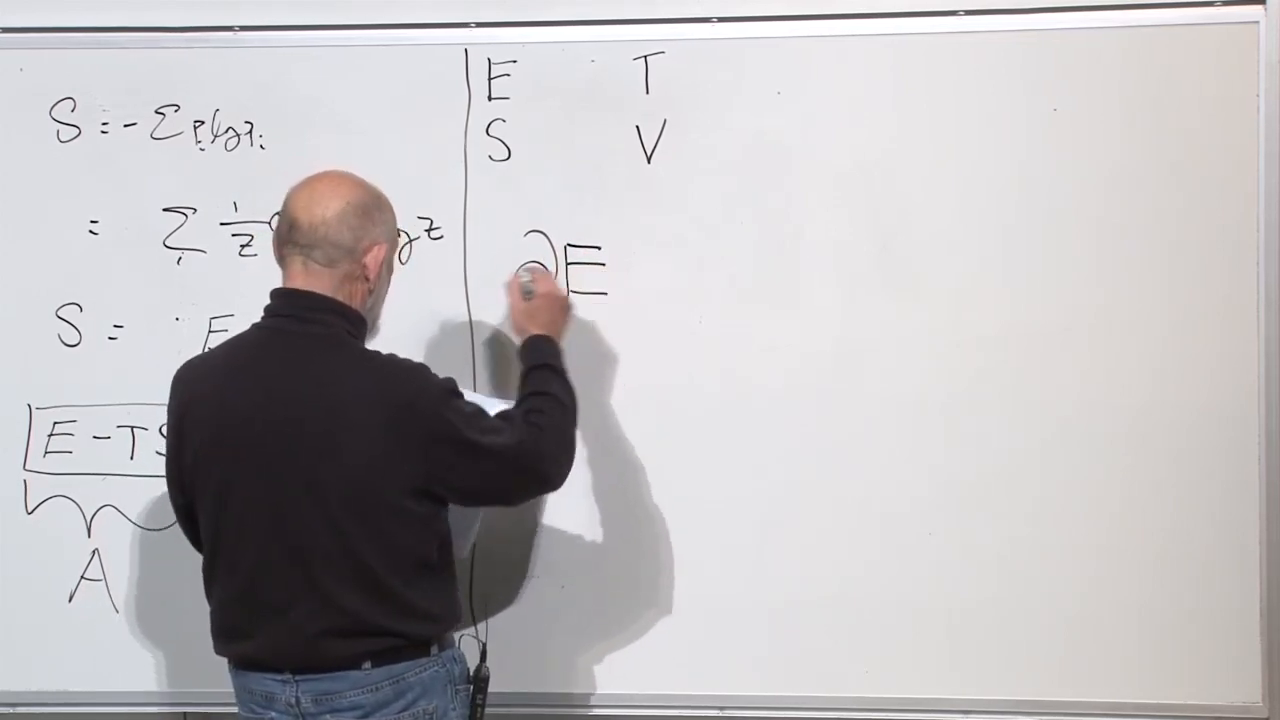
\includegraphics[width=0.90\textwidth]{lecture_05_figure_03.png}\caption{La relación canónica para la entropía reordenada como \(A=E-TS=-T\log Z\).}\lectureframe{00:16:50}\end{figure}

\section{Parámetros de control y sus respuestas}

Un parámetro de control es una magnitud macroscópica que un experimentador puede modificar desde el exterior. Al mover un pistón se cambia el volumen sin manipular moléculas individuales. Los campos eléctricos y magnéticos aplicados son otros ejemplos. En un ensamble más general también se puede permitir que cambie el número de partículas.

Las variables termodinámicas se presentan naturalmente en pares conjugados. En el problema actual, el volumen es el parámetro de control y la presión su respuesta. Cambiamos \(V\); la presión indica cómo se opone energéticamente el sistema a ese cambio. Más adelante, la derivada de la energía precisará esta relación.

\begin{classroomqa}\audiencequestion{¿Puede considerarse la presión misma como parámetro de control?}\lecturerresponse{Se puede diseñar un experimento que mantenga fija la presión externa, pero en el montaje que usamos aquí la posición del pistón fija el volumen y la presión interna es la respuesta. La presión y el volumen son variables conjugadas; cuál de ellas se controla depende del ensamble y del aparato. \lecturetimestamp{00:19:22--00:20:01}}\end{classroomqa}

\begin{classroomqa}\audiencequestion{¿Se supone que todas las moléculas son idénticas o el argumento se limita a un gas?}\lecturerresponse{El argumento termodinámico no requiere ninguna de esas restricciones. El cilindro puede contener varias especies, un líquido o incluso un sólido sometido a compresión. La función de partición del gas ideal será solo una aplicación particular, después de establecer la fórmula general de la presión. \lecturetimestamp{00:20:02--00:20:39}}\end{classroomqa}

\begin{classroomqa}\audiencequestion{¿Se podría cambiar la cantidad de sustancia mediante otra operación externa?}\lecturerresponse{Sí. El número de partículas es otro posible parámetro de control. Si se trata dinámicamente, aparece su propia variable conjugada: el potencial químico. Para el cálculo de hoy, \(N\) permanece fijo. \lecturetimestamp{00:20:39--00:20:57}}\end{classroomqa}

\begin{classroomqa}\audiencequestion{¿Pueden coexistir en equilibrio el agua líquida y el vapor?}\lecturerresponse{Pueden hacerlo a la temperatura y presión de coexistencia. La gravedad puede situar el líquido debajo del vapor y, aun así, ambas fases pueden compartir una misma temperatura y permanecer en equilibrio térmico. Se aplica el mismo marco general de la mecánica estadística. \lecturetimestamp{00:20:59--00:21:36}}\end{classroomqa}

Para el siguiente argumento, consideremos la energía y la entropía como funciones dependientes de dos variables que se pueden ajustar independientemente: \begin{equation}
 E=E(T,V),
 \qquad
 S=S(T,V).
 \label{eq:sm5-dependent-functions}
\end{equation} La temperatura y el volumen proporcionan coordenadas en el espacio de estados termodinámicos. La energía y la entropía asignan valores a cada punto de equilibrio de ese espacio.

\section{La derivada a entropía constante}

La derivada que necesitamos en última instancia es poco habitual: \[
 \left(\frac{\partial E}{\partial V}\right)_S.
\] Aunque \(T\) y \(V\) son las coordenadas independientes, esta derivada pide variar \(V\) mientras se impone que la función dependiente \(S(T,V)\) permanezca constante. Es una derivada a lo largo de una curva en el plano \((T,V)\), no a lo largo de un eje de coordenadas.

\begin{classroomqa}\audiencequestion{¿Cómo pueden ser independientes \(T\) y \(V\) si más adelante se usa una derivada \(dT/dV\)?}\lecturerresponse{Son independientes en el espacio de estados completo. Al imponer la restricción \(S(T,V)=\mathrm{constant}\), los estados permitidos quedan sobre una curva unidimensional. A lo largo de esa curva, \(T\) pasa a ser función de \(V\) y su pendiente \(dT/dV\) está bien definida. \lecturetimestamp{01:01:18--01:02:09}}\end{classroomqa}

\begin{lemma}Si \(E(T,V)\) y \(S(T,V)\) son diferenciables, entonces, dondequiera que \((\partial S/\partial T)_V\neq0\): \begin{equation}
 \left(\frac{\partial E}{\partial V}\right)_S
 =
 \left(\frac{\partial E}{\partial V}\right)_T
 -
 \left(\frac{\partial E}{\partial S}\right)_V
 \left(\frac{\partial S}{\partial V}\right)_T.
 \label{eq:sm5-calculus-lemma}
\end{equation}\end{lemma}

\begin{proof}Para un desplazamiento infinitesimal arbitrario: \begin{equation}
 dE=
 \left(\frac{\partial E}{\partial V}\right)_T dV
 +
 \left(\frac{\partial E}{\partial T}\right)_V dT.
 \label{eq:sm5-total-differential-e}
\end{equation} A \(V\) constante, la regla de la cadena permite usar \(S\) como variable intermedia: \begin{equation}
 \left(\frac{\partial E}{\partial T}\right)_V
 =
 \left(\frac{\partial E}{\partial S}\right)_V
 \left(\frac{\partial S}{\partial T}\right)_V.
 \label{eq:sm5-chain-rule-e-s-t}
\end{equation}

Restringimos ahora el desplazamiento a una curva en la que \(S\) es constante. A lo largo de esa curva, \begin{equation}
 0=dS=
 \left(\frac{\partial S}{\partial V}\right)_T dV
 +
 \left(\frac{\partial S}{\partial T}\right)_V dT.
 \label{eq:sm5-constant-entropy-differential}
\end{equation} Despejando la pendiente de la curva se obtiene \begin{equation}
 \left(\frac{dT}{dV}\right)_S
 =
 -
 \frac{\left(\frac{\partial S}{\partial V}\right)_T}
 {\left(\frac{\partial S}{\partial T}\right)_V}.
 \label{eq:sm5-entropy-contour-slope}
\end{equation} Dividimos \eqref{eq:sm5-total-differential-e} por \(dV\), usamos \eqref{eq:sm5-chain-rule-e-s-t} e insertamos \eqref{eq:sm5-entropy-contour-slope}: \begin{align}
 \left(\frac{\partial E}{\partial V}\right)_S
 &=
 \left(\frac{\partial E}{\partial V}\right)_T
 +
 \left(\frac{\partial E}{\partial S}\right)_V
 \left(\frac{\partial S}{\partial T}\right)_V
 \left(\frac{dT}{dV}\right)_S \notag\\
 &=
 \left(\frac{\partial E}{\partial V}\right)_T
 -
 \left(\frac{\partial E}{\partial S}\right)_V
 \left(\frac{\partial S}{\partial V}\right)_T.
\end{align} El factor \((\partial S/\partial T)_V\) se ha cancelado, lo que demuestra el resultado. \end{proof}

\begin{figure}[t]\centering
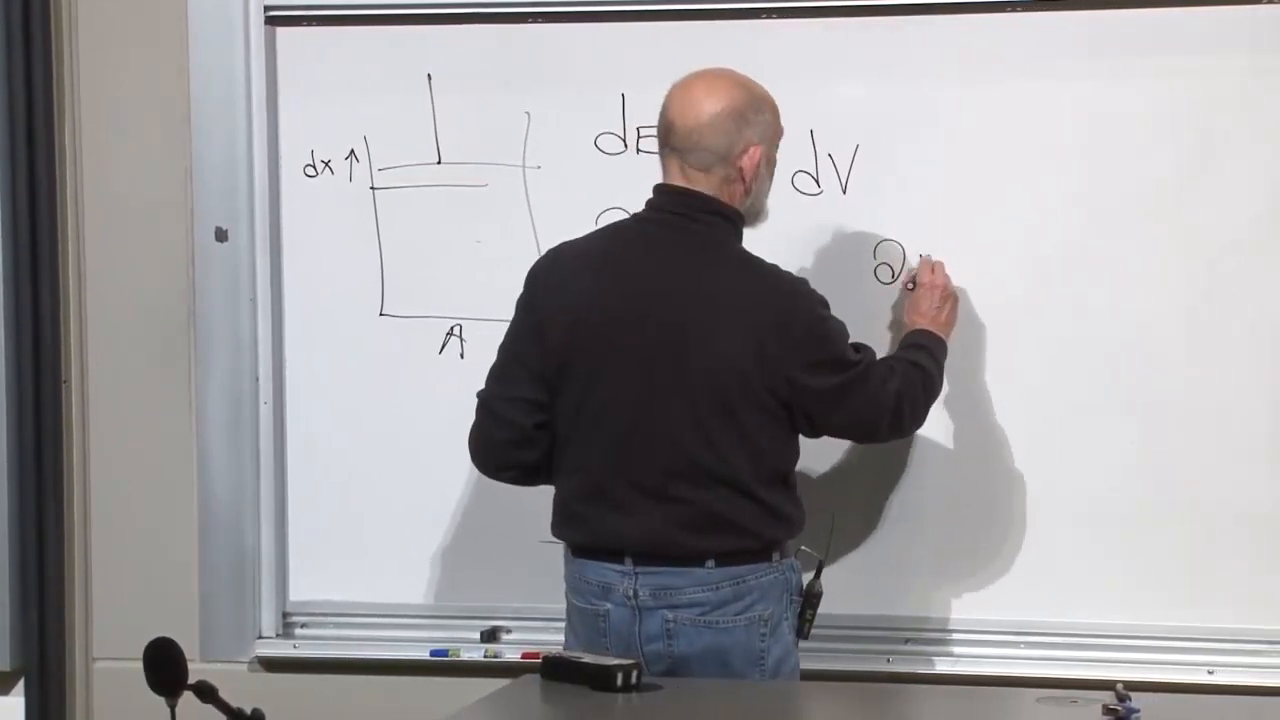
\includegraphics[width=0.90\textwidth]{lecture_05_figure_04.png}\caption{Cálculo sobre la curva de entropía constante, en el punto de cancelación que completa el lema sobre derivadas.}\lectureframe{00:36:10}\end{figure}

La interpretación geométrica no es un mero adorno. Explica por qué una derivada a \(S\) constante que parece extraña se puede calcular mediante derivadas parciales ordinarias en las coordenadas independientes \(T\) y \(V\). Escribir \(\delta E/\delta V\) durante la construcción sirve para recordar que los símbolos representan cocientes de cambios pequeños a lo largo de una trayectoria especificada.

\begin{classroomqa}\audiencequestion{¿El desarrollo de \(dE\) es simplemente la definición habitual de las derivadas parciales?}\lecturerresponse{Sí. En el diferencial total no hay nada especial. El único ingrediente adicional es la restricción posterior a la curva \(dS=0\), que determina la relación entre \(dT\) y \(dV\). \lecturetimestamp{00:29:26--00:29:32}}\end{classroomqa}

\begin{classroomqa}\audiencequestion{¿La cancelación requiere que \((\partial S/\partial T)_V\) sea distinto de cero?}\lecturerresponse{Sí. Para un sistema estable ordinario, \[
 \left(\frac{\partial S}{\partial T}\right)_V
 =\frac{C_V}{T}>0,
\] así que la división está justificada. Los puntos excepcionales requieren un análisis aparte. Con el Hamiltoniano fijo, elevar la temperatura ensancha la distribución canónica de energía y normalmente aumenta la entropía; bajar la temperatura la estrecha. Esta es la orientación físicamente correcta del argumento de monotonía. \lecturetimestamp{00:36:50--00:37:47}}\end{classroomqa}

\section{Trabajo del pistón y condición adiabática}

Ahora daremos un significado físico a la derivada. Consideremos un pistón de área transversal \(\mathcal A\). Si se desplaza hacia fuera una distancia \(dx\), entonces \begin{equation}
 dV=\mathcal A\,dx.
 \label{eq:sm5-piston-volume}
\end{equation} El gas ejerce sobre el pistón una fuerza \(P\mathcal A\), de modo que el trabajo realizado por el gas es \begin{equation}
 \delta W_{\mathrm{by}}=P\mathcal A\,dx=P\,dV.
 \label{eq:sm5-piston-work}
\end{equation} Si no entra calor en el gas, la conservación de la energía da \begin{equation}
 dE=-P\,dV.
 \label{eq:sm5-adiabatic-work}
\end{equation} El signo tiene un significado físico: durante la expansión, el gas eleva el pistón o lo acelera, y su propia energía disminuye.

\begin{figure}[t]\centering
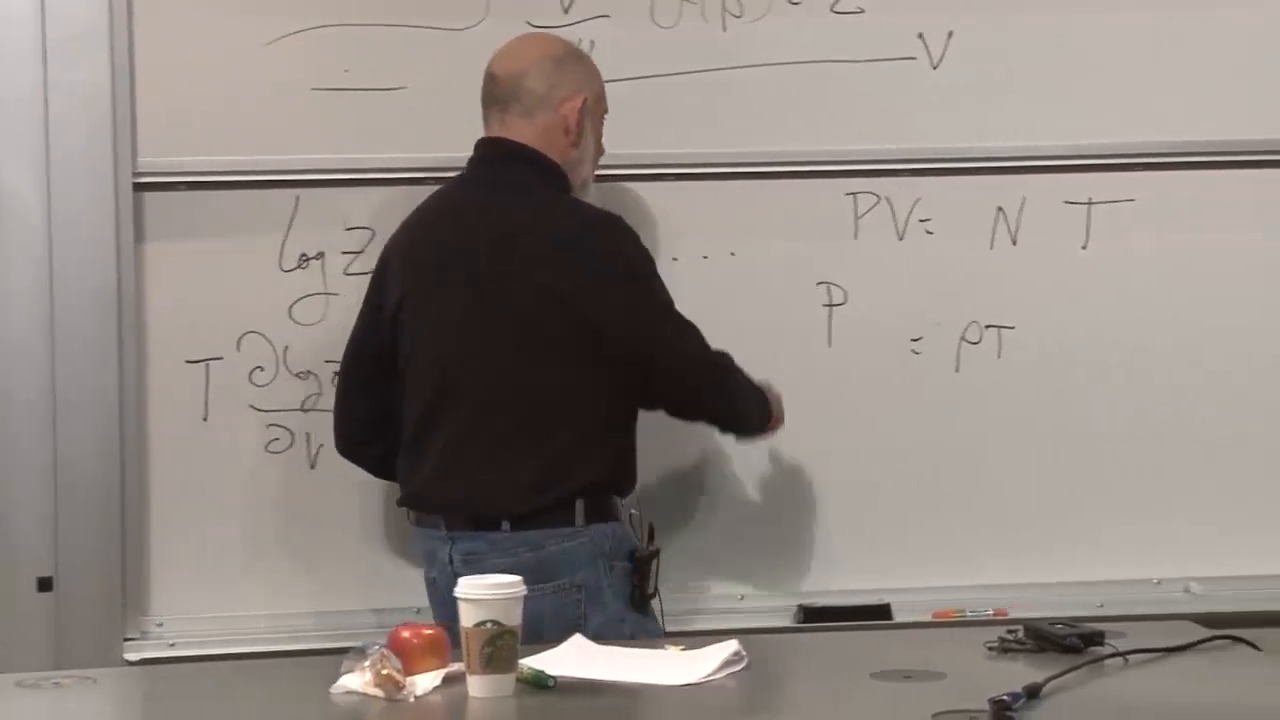
\includegraphics[width=0.90\textwidth]{lecture_05_figure_05.png}\caption{Geometría del pistón y relación de trabajo resultante \(dE=-P\,dV\).}\lectureframe{00:43:10}\end{figure}

Hay dos condiciones esenciales. El pistón debe moverse con suficiente lentitud para que el sistema permanezca tan cerca del equilibrio como se quiera, y las paredes deben estar aisladas para que no se suministre energía en forma de calor. Una tracción rápida puede ser tan breve que ninguna molécula alcance el pistón, que se aleja, durante el movimiento. Una compresión rápida genera ondas de choque. Ninguno de estos procesos se representa mediante una sucesión de estados de equilibrio.

A veces se usa la palabra \emph{adiabático} para indicar ausencia de transferencia de calor y otras veces para indicar un cambio lento. En el proceso reversible que necesitamos intervienen ambas ideas: el cambio es cuasiestático y térmicamente aislado. En esas condiciones, también es isentrópico.

\begin{classroomqa}\audiencequestion{¿Por qué un cambio adiabático mantiene constante la entropía?}\lecturerresponse{Consideremos el sistema desde el punto de vista de la mecánica cuántica. Sus niveles de energía de muchos cuerpos dependen del volumen. Cuando \(V\) cambia lentamente, el teorema adiabático lleva cada nivel ocupado de manera continua a su nivel sucesor, sin transiciones entre las etiquetas de los niveles. Las energías \(E_i(V)\) cambian, pero las probabilidades de ocupación \(p_i\) permanecen fijas. Como \(S=-\sum_i p_i\log p_i\) depende de esas probabilidades, la entropía permanece constante. El intercambio de calor o el movimiento irreversible invalidarían esta conclusión. \lecturetimestamp{00:43:37--00:49:15}}\end{classroomqa}

\begin{figure}[t]\centering
\includegraphics[width=0.90\textwidth]{lecture_05_figure_06.png}\caption{Niveles de energía de muchos cuerpos que varían con el volumen mientras sus probabilidades de ocupación conservan las etiquetas de los niveles.}\lectureframe{00:48:50}\end{figure}

La ecuación \eqref{eq:sm5-adiabatic-work}, evaluada a lo largo de esta trayectoria de entropía constante, identifica la presión como \begin{equation}
 P=-\left(\frac{\partial E}{\partial V}\right)_S.
 \label{eq:sm5-pressure-fixed-entropy}
\end{equation} Esta es la relación conjugada entre presión y volumen.

\begin{classroomqa}\audiencequestion{¿Qué ocurre si el pistón se mueve rápidamente?}\lecturerresponse{El sistema deja de estar en equilibrio y su dinámica detallada pasa a ser relevante. Una compresión brusca genera una onda de choque. En una expansión libre ideal, el pistón puede alejarse antes de que ninguna molécula choque contra él, por lo que no se realiza trabajo y la energía permanece constante aunque cambie el volumen. Después, el gas se relaja hasta alcanzar el equilibrio y su entropía aumenta. Estos procesos no pueden describirse mediante la única derivada de equilibrio en \eqref{eq:sm5-pressure-fixed-entropy}. \lecturetimestamp{00:58:30--01:01:15}}\end{classroomqa}

\begin{classroomqa}\audiencequestion{¿Qué condición cuantitativa determina si un cambio es lento?}\lecturerresponse{El tiempo de variación externa debe ser largo en comparación con los tiempos de relajación internos pertinentes. En un gas, durante el cambio macroscópico deberían producirse muchas colisiones moleculares y muchos choques contra las paredes. La escala temporal precisa depende del material y la geometría, mientras que el límite cuasiestático es general. \lecturetimestamp{01:02:09--01:03:20}}\end{classroomqa}

\section{De la energía adiabática a la función de partición}

La fórmula física \eqref{eq:sm5-pressure-fixed-entropy} todavía no es la más fácil de calcular. La mecánica estadística canónica proporciona naturalmente funciones de la temperatura, porque \(T\) aparece directamente en el factor de Boltzmann. El lema de cálculo transforma la incómoda derivada a entropía constante en una forma que facilita el cálculo: \begin{align}
 P
 &=
 -\left(\frac{\partial E}{\partial V}\right)_T
 +
 \left(\frac{\partial E}{\partial S}\right)_V
 \left(\frac{\partial S}{\partial V}\right)_T.
 \label{eq:sm5-pressure-lemma-substitution}
\end{align} A volumen constante, la primera ley da \(dE=T\,dS\) y, por tanto, \begin{equation}
 \left(\frac{\partial E}{\partial S}\right)_V=T.
 \label{eq:sm5-e-s-temperature}
\end{equation} Así pues: \begin{equation}
 P=
 -\left(\frac{\partial E}{\partial V}\right)_T
 +
 T\left(\frac{\partial S}{\partial V}\right)_T.
 \label{eq:sm5-pressure-fixed-temperature-pieces}
\end{equation}

\begin{classroomqa}\audiencequestion{¿De dónde viene el signo menos de la fórmula de la presión?}\lecturerresponse{Se origina en el trabajo realizado por el gas: \(dE=-P\,dV\) durante la expansión adiabática. El lema de cálculo tiene por sí mismo un signo menos entre sus dos términos; el signo menos global de \(P=-(\partial E/\partial V)_S\) cambia el signo de ambos, y se obtiene \eqref{eq:sm5-pressure-fixed-temperature-pieces}. \lecturetimestamp{00:52:40--00:53:14}}\end{classroomqa}

Como \(T\) se mantiene fijo en ambas derivadas, \begin{align}
 P
 &=
 -\left(\frac{\partial}{\partial V}(E-TS)\right)_T \notag\\
 &=
 -\left(\frac{\partial A}{\partial V}\right)_T.
 \label{eq:sm5-pressure-free-energy}
\end{align} Por último, sustituimos \(A=-T\log Z\): \begin{equation}
 \boxed{
 P=
 T\left(\frac{\partial\log Z}{\partial V}\right)_T
 }.
 \label{eq:sm5-pressure-log-z}
\end{equation}

\begin{figure}[t]\centering
\includegraphics[width=0.90\textwidth]{lecture_05_figure_07.png}\caption{Compresión del argumento a temperatura constante: \(P=-(\partial A/\partial V)_T
=T(\partial\log Z/\partial V)_T\).}\lectureframe{00:55:55}\end{figure}

Nada en \eqref{eq:sm5-pressure-log-z} presupone que el gas sea ideal. Si se puede calcular la función de partición de un fluido interactuante, un plasma o un sólido, la misma derivada da su presión. En términos más generales, cada parámetro de control externo tiene una respuesta conjugada que se obtiene derivando un potencial termodinámico apropiado. La función de partición reúne muchas de esas respuestas: derivar \(\log Z\) con respecto a \(\beta\) da la energía, mientras que derivarla con respecto al volumen da la presión.

\section{La ecuación de estado del gas ideal}

Solo ahora nos restringimos a \(N\) partículas no interactuantes. Conservando la normalización clásica del espacio de fases, \begin{equation}
 Z_N=
 \frac{1}{N!h^{3N}}
 \int d^{3N}q\,d^{3N}p\,
 \exp\!\left[
 -\beta\sum_{a=1}^{N}\frac{\mathbf p_a^2}{2m}
 \right].
 \label{eq:sm5-ideal-gas-partition-integral}
\end{equation} Hay \(3N\) coordenadas de posición y \(3N\) coordenadas de momento. El Hamiltoniano no depende de la posición, por lo que cada partícula aporta un factor igual al volumen del recipiente: \begin{equation}
 Z_N=
 \frac{V^N}{N!h^{3N}}I_p(\beta),
 \label{eq:sm5-ideal-gas-factorization}
\end{equation} donde la integral de momento completa \(I_p(\beta)\) no depende de \(V\).

\begin{classroomqa}\audiencequestion{¿Por qué hay \(3N\) integrales de posición y \(3N\) integrales de momento?}\lecturerresponse{Cada una de las \(N\) partículas tiene tres coordenadas espaciales y tres componentes de momento conjugadas. El número es \(3N\) en cada mitad del espacio de fases, no \(N\) partículas más otras \(3N\) partículas. \lecturetimestamp{01:04:19--01:04:28}}\end{classroomqa}

Al tomar el logaritmo se separa la dependencia del volumen: \begin{equation}
 \log Z_N
 =
 N\log V-\log N!-3N\log h+\log I_p(\beta).
 \label{eq:sm5-log-ideal-gas-partition}
\end{equation} Los factores \(1/N!\), \(h^{-3N}\) y \(I_p(\beta)\) son todos independientes del volumen. Importan para la entropía absoluta y otras cuestiones, pero no para esta derivada concreta. Por tanto, \begin{equation}
 \left(\frac{\partial\log Z_N}{\partial V}\right)_T
 =\frac{N}{V}.
 \label{eq:sm5-log-z-volume-derivative}
\end{equation} La ecuación \eqref{eq:sm5-pressure-log-z} da inmediatamente \begin{equation}
 P=\frac{NT}{V},
 \qquad
 \boxed{PV=NT}.
 \label{eq:sm5-ideal-gas-law}
\end{equation}

\begin{classroomqa}\audiencequestion{¿Sigue \(N\) contando las réplicas usadas para derivar la distribución de Boltzmann?}\lecturerresponse{No. La construcción con réplicas fue un recurso de conteo en la derivación anterior y ya no interviene. Aquí, \(N\) es el número de partículas físicas de esta muestra de gas. \lecturetimestamp{01:07:38--01:08:05}}\end{classroomqa}

Al definir la densidad numérica \begin{equation}
 \rho=\frac{N}{V}
 \label{eq:sm5-number-density}
\end{equation} se obtiene la forma equivalente \begin{equation}
 P=\rho T.
 \label{eq:sm5-density-equation-of-state}
\end{equation}

\begin{classroomqa}\audiencequestion{¿Se obtiene la expresión en términos de la densidad dividiendo por \(N\) o por \(V\)?}\lecturerresponse{Dividimos \(PV=NT\) por \(V\): \(P=(N/V)T=\rho T\). Aquí \(\rho\) es la densidad numérica, no la densidad de masa. \lecturetimestamp{01:08:45--01:09:16}}\end{classroomqa}

\begin{figure}[t]\centering
\includegraphics[width=0.90\textwidth]{lecture_05_figure_08.png}\caption{La derivada respecto al volumen de \(\log Z\) y la ecuación de estado resultante del gas ideal \(PV=NT\), o bien \(P=\rho T\).}\lectureframe{01:09:25}\end{figure}

Al recuperar la temperatura de laboratorio \(T_K\): \begin{equation}
 PV=Nk_BT_K.
 \label{eq:sm5-ideal-gas-law-laboratory}
\end{equation} El resultado conocido concuerda con la intuición cinética, pero su derivación se apoya ahora en un marco que va mucho más allá del gas libre.

\section{Un segundo fruto: las fluctuaciones de equilibrio}

El cálculo de la presión está completo, pero queda una pregunta que habíamos prometido responder: ¿qué más se puede extraer de la función de partición? Consideremos un sistema en contacto térmico con un baño de calor. Su energía no es fija. La energía entra y sale, por lo que las mediciones repetidas fluctúan alrededor de la media canónica.

\begin{classroomqa}\audiencequestion{¿Podemos calcular ahora las fluctuaciones prometidas?}\lecturerresponse{Sí. El tiempo adicional permite una segunda demostración del mismo principio: las derivadas de \(Z\) codifican información termodinámica medible. \lecturetimestamp{01:10:37--01:10:50}}\end{classroomqa}

\subsection{Varianza y desviación estándar}

Para una variable aleatoria \(x\) con \(\langle x\rangle=0\), una medida de la amplitud de la distribución es \(\langle x^2\rangle\). Para una distribución general, desplazamos la variable restándole su media: \begin{equation}
 \delta x=x-\langle x\rangle.
 \label{eq:sm5-centered-variable}
\end{equation} Su media es cero: \begin{equation}
 \langle\delta x\rangle
 =
 \langle x\rangle-\langle x\rangle=0,
 \label{eq:sm5-centered-mean}
\end{equation} y su media cuadrática es \begin{align}
 (\Delta x)^2
 &\equiv
 \left\langle\left(x-\langle x\rangle\right)^2\right\rangle \notag\\
 &=
 \langle x^2\rangle
 -2\langle x\rangle^2
 +\langle x\rangle^2 \notag\\
 &=
 \langle x^2\rangle-\langle x\rangle^2.
 \label{eq:sm5-variance}
\end{align} Esta es la varianza. Su raíz cuadrada positiva \(\Delta x\) es la desviación estándar.

\begin{classroomqa}\audiencequestion{¿Por qué el promedio de \(x-\langle x\rangle\) es exactamente cero?}\lecturerresponse{Los promedios son lineales, y \(\langle x\rangle\) ya es un número. Por tanto, \(\langle x-\langle x\rangle\rangle
=\langle x\rangle-\langle x\rangle=0\). \lecturetimestamp{01:14:02--01:14:22}}\end{classroomqa}

\begin{classroomqa}\audiencequestion{¿Qué diferencia hay entre fluctuación cuadrática, varianza, amplitud cuadrática media y desviación estándar?}\lecturerresponse{La varianza es \((\Delta x)^2=\langle x^2\rangle-\langle x\rangle^2\). La desviación estándar es su raíz cuadrada, \(\Delta x\). Para una variable de media cero, la desviación estándar también es su valor cuadrático medio. \lecturetimestamp{01:16:39--01:18:38}}\end{classroomqa}

\begin{figure}[t]\centering
\includegraphics[width=0.90\textwidth]{lecture_05_figure_09.png}\caption{La variable centrada y el desarrollo que da lugar a \((\Delta x)^2=\langle x^2\rangle-\langle x\rangle^2\).}\lectureframe{01:17:20}\end{figure}

\subsection{Momentos de energía a partir de la función de partición}

Para el ensamble canónico, \begin{align}
 \langle E\rangle
 &=
 \frac{1}{Z}\sum_i E_i e^{-\beta E_i} \notag\\
 &=
 -\frac{1}{Z}\frac{\partial Z}{\partial\beta}
 =
 -\frac{\partial\log Z}{\partial\beta}.
 \label{eq:sm5-mean-energy-from-z}
\end{align} La multiplicación por un factor \(E_i\) se obtiene mediante una derivada negativa respecto de \(\beta\). Una segunda derivada genera \(E_i^2\): \begin{equation}
 \langle E^2\rangle
 =
 \frac{1}{Z}\sum_i E_i^2e^{-\beta E_i}
 =
 \frac{1}{Z}\frac{\partial^2 Z}{\partial\beta^2}.
 \label{eq:sm5-second-energy-moment}
\end{equation} En consecuencia, la varianza de la energía es \begin{align}
 (\Delta E)^2
 &=
 \langle E^2\rangle-\langle E\rangle^2 \notag\\
 &=
 \frac{1}{Z}\frac{\partial^2Z}{\partial\beta^2}
 -
 \frac{1}{Z^2}
 \left(\frac{\partial Z}{\partial\beta}\right)^2 \notag\\
 &=
 \frac{\partial^2\log Z}{\partial\beta^2}
 =
 -\frac{\partial\langle E\rangle}{\partial\beta}.
 \label{eq:sm5-energy-variance-beta}
\end{align} Una vez más, un observable que parece complicado se convierte en una derivada de \(\log Z\).

\begin{figure}[t]\centering
\includegraphics[width=0.90\textwidth]{lecture_05_figure_10.png}\caption{La segunda derivada respecto de \(\beta\) de \(\log Z\), identificada con la varianza de la energía.}\lectureframe{01:29:00}\end{figure}

\subsection{Capacidad calorífica y magnitud de las fluctuaciones}

En las unidades usadas en la clase, \(T=1/\beta\), de modo que \begin{equation}
 -\frac{\partial}{\partial\beta}
 =
 T^2\frac{\partial}{\partial T}.
 \label{eq:sm5-beta-temperature-derivative}
\end{equation} A volumen constante, definimos la capacidad calorífica de la muestra completa como \begin{equation}
 C_V\equiv
 \left(\frac{\partial\langle E\rangle}{\partial T}\right)_V.
 \label{eq:sm5-heat-capacity}
\end{equation} La ecuación \eqref{eq:sm5-energy-variance-beta} queda \begin{equation}
 \boxed{(\Delta E)^2=T^2C_V}
 \qquad (k_B=1).
 \label{eq:sm5-energy-fluctuation-lecture-units}
\end{equation} Para la temperatura de laboratorio \(T_K\), donde \(\beta=(k_BT_K)^{-1}\), \begin{equation}
 \boxed{(\Delta E)^2=k_BT_K^2C_V}.
 \label{eq:sm5-energy-fluctuation-laboratory}
\end{equation}

\begin{figure}[t]\centering
\includegraphics[width=0.90\textwidth]{lecture_05_figure_11.png}\caption{Conversión de la derivada respecto de \(\beta\) a la capacidad calorífica a volumen constante, incluido el factor \(k_B\) restituido.}\lectureframe{01:31:10}\end{figure}

\begin{classroomqa}\audiencequestion{¿La derivada debe especificar volumen constante en vez de presión constante?}\lecturerresponse{Sí. Esta derivación canónica mantiene fijos los parámetros de control externos del Hamiltoniano, incluido \(V\). La magnitud resultante es \(C_V\). En un ensamble a presión constante, el volumen y el trabajo pueden fluctuar, y se necesita el potencial termodinámico correspondiente; no se puede sustituir simplemente \(C_V\) por \(C_P\) en \eqref{eq:sm5-energy-fluctuation-laboratory}. \lecturetimestamp{01:29:01--01:29:28; 01:32:50--01:33:21}}\end{classroomqa}

\begin{classroomqa}\audiencequestion{¿Es \(C_V\) una constante del material?}\lecturerresponse{En general, no. Puede depender de la temperatura, el volumen, la fase y la composición. Además, \(C_V\) es aquí la capacidad calorífica de la muestra completa y es extensiva. El calor específico se obtiene solo al dividir por la masa, el número de partículas o la cantidad de sustancia. \lecturetimestamp{01:31:47--01:32:21; 01:33:23--01:34:55}}\end{classroomqa}

Para la materia extensiva ordinaria, \(C_V\) es proporcional a \(N\), por lo que \((\Delta E)^2\) es proporcional a \(N\) y \(\Delta E\) a \(\sqrt{N}\). La energía media es proporcional a \(N\). Por tanto, \begin{equation}
 \frac{\Delta E}{\langle E\rangle}\sim\frac{1}{\sqrt{N}}.
 \label{eq:sm5-relative-fluctuation-scaling}
\end{equation} Las fluctuaciones relativas son minúsculas a escala macroscópica, mientras que en muestras microscópicas se manifiestan directamente. La aparición de \(k_B\) en \eqref{eq:sm5-energy-fluctuation-laboratory} señala esta conexión entre los observables termodinámicos y la granularidad molecular; equivalentemente, conecta las unidades macroscópicas con el conteo a escala de Avogadro.

La presión y las fluctuaciones han surgido ahora del mismo objeto: \[
 P=T\left(\frac{\partial\log Z}{\partial V}\right)_T,
 \qquad
 (\Delta E)^2=\frac{\partial^2\log Z}{\partial\beta^2}.
\] Esta es la lección central. Una vez identificadas las restricciones correctas, la función de partición no se limita a normalizar probabilidades. Sus derivadas organizan la termodinámica medible del sistema.
\chapter{Interacciones débiles, correcciones viriales y diferenciales inexactas}

\lectureoverview{Comenzamos por el significado operacional de la medición y la temperatura; después preguntamos cómo se aparta un gas diluido de la ley de los gases ideales cuando se activan débilmente interacciones de corto alcance. La función de partición proporciona las primeras correcciones de la interacción a la energía y la presión, e identifica el intervalo en que son válidas. Al final, una digresión matemática distingue las funciones de estado del calor y el trabajo, que dependen de la trayectoria, mediante diferenciales exactas, lazos cerrados y una prueba concreta con un gas ideal.}

\section{Qué mide realmente un instrumento}

Ningún instrumento de laboratorio se adentra directamente en la naturaleza para informar de una variable matemática abstracta. Una balanza de resorte indica un alargamiento; un termómetro, la altura de una columna de líquido. Decimos que la primera mide una fuerza y el segundo una temperatura solo porque se ha establecido una relación reproducible entre la respuesta observable y la magnitud buscada.

Esa relación solo es válida en un intervalo limitado. Un resorte obedece la ley de Hooke mientras permanece elástico, pero una fuerza suficientemente grande acaba por deformarlo o romperlo. En general, si una lectura suave \(R\) depende de una variable física \(X\), cerca de un punto de funcionamiento elegido se cumple \begin{equation}
 \Delta R \simeq
 \left.\frac{dR}{dX}\right|_{X_0}\Delta X.
 \label{eq:sm6-local-linear-response}
\end{equation} Los pequeños cambios en la lectura son proporcionales a los pequeños cambios en la variable buscada, incluso si la curva de respuesta completa es no lineal. Esta linealización local es la lógica habitual de la calibración.

La lectura también puede depender de variables perturbadoras. Un resorte puede responder débilmente a la temperatura o a la presión. La altura del mercurio en un termómetro podría depender de la orientación por efecto de la gravedad, de las propiedades del vidrio o de cambios lentos en los materiales. Un protocolo de medición no demuestra que estas dependencias no existan: las mantiene constantes o muestra que son despreciables a la escala requerida.

\begin{classroomqa}\audiencequestion{¿Podrían el campo gravitatorio local o la dirección en que se sostiene el termómetro cambiar la lectura?}\lecturerresponse{En principio, sí. Si la orientación tiene un efecto apreciable, la instrucción de sostener el termómetro en posición vertical pasa a formar parte de la definición del instrumento. Cerca de la superficie terrestre, el campo gravitatorio es suficientemente estable como para que las variaciones restantes sean normalmente despreciables.\lecturetimestamp{00:04:08--00:05:00}}\end{classroomqa}

\begin{classroomqa}\audiencequestion{¿Podrían el envejecimiento o los cambios químicos alterar gradualmente la calibración?}\lecturerresponse{Podrían. El mercurio y el vidrio son suficientemente inertes para las mediciones habituales, mientras que los cambios a escalas de tiempo extraordinariamente largas son irrelevantes para el experimento. Toda calibración se refiere a un instrumento, un intervalo, un protocolo y una duración especificados.\lecturetimestamp{00:05:03--00:06:11}}\end{classroomqa}

En un termómetro Celsius, dos estados de referencia reproducibles proporcionan una escala práctica. Si \(h_f\) y \(h_b\) son, respectivamente, las alturas de la columna en los puntos de congelación y ebullición del agua, dentro de un intervalo en el que la respuesta es casi lineal, \begin{equation}
 T_{\mathrm C}=100\,\frac{h-h_f}{h_b-h_f}.
 \label{eq:sm6-celsius-calibration}
\end{equation} La elección de \(T_{\mathrm C}=0\) en el punto de congelación es convencional. No representa el estado de energía térmica nula, del mismo modo que cero grados Fahrenheit en un día de invierno no es el cero absoluto.

\begin{figure}[t]\centering
\includegraphics[width=0.90\textwidth]{lecture_06_figure_03.png}\caption{Respuesta suave pero no lineal de un termómetro, con un intervalo breve delimitado para la calibración lineal.}\lectureframe{00:07:55}\end{figure}

\section{El equilibrio y la temperatura como escala de energía}

Un termómetro mide la temperatura de lo que lo rodea solo después de que el termómetro y el medio cercano hayan alcanzado el equilibrio térmico. Antes de eso, su lectura simplemente está cambiando hacia el equilibrio. La prueba práctica es sencilla: esperar hasta que la lectura deje de cambiar. Esa regla tan simple oculta los procesos físicos que determinan el tiempo de espera.

\begin{classroomqa}\audiencequestion{¿La equilibración ocurre solo en una capa límite alrededor del bulbo, y cuánto hay que esperar?}\lecturerresponse{La energía debe atravesar el vidrio e intercambiarse con el medio circundante, así que el tiempo depende del termómetro, de su conductividad térmica y del medio. El entorno inmediato también debe ser representativo de un estado de equilibrio uniforme. En la práctica, se acepta la lectura cuando ha dejado de variar.\lecturetimestamp{00:08:45--00:10:13}}\end{classroomqa}

La temperatura y la densidad desempeñan papeles distintos en este tiempo de espera. Un gas muy diluido puede estar muy caliente: las pocas moléculas presentes pueden tener grandes energías cinéticas. Sin embargo, esas moléculas chocan pocas veces con el termómetro, por lo que la equilibración puede ser lenta. Reducir la densidad por un factor de cien o mil manteniendo fija la temperatura no reduce la escala de energía molecular; reduce la rapidez con que esa energía se comunica al instrumento.

\begin{classroomqa}\audiencequestion{¿Puede la radiación de una habitación tener una temperatura distinta de la del aire?}\lecturerresponse{Sí. La materia y la radiación comparten una misma temperatura solo cuando están en equilibrio térmico entre sí. El aire neutro se acopla débilmente a gran parte de la radiación óptica de una habitación iluminada, y la población de fotones no tiene por qué constituir un campo de radiación de cuerpo negro en equilibrio a la temperatura del aire.\lecturetimestamp{00:11:26--00:12:20}}\end{classroomqa}

Una vez establecido el equilibrio, conviene considerar la temperatura como una escala de energía. Seguimos usando unidades en las que \(k_B=1\), de modo que \(T\) tiene dimensiones de energía. Para un gas ideal monoatómico, \begin{equation}
 E_0=\frac{3}{2}NT.
 \label{eq:sm6-ideal-energy}
\end{equation} La energía térmica por molécula queda fijada por \(T\); la rapidez correspondiente sigue dependiendo de la masa molecular.

\section{Activación de una interacción débil}

\begin{classroomqa}\audiencequestion{¿En qué condiciones deja de ser válida la aproximación de gas ideal, y puede mostrarse matemáticamente ese fallo?}\lecturerresponse{Partamos del gas no interactuante ya resuelto y activemos una interacción pequeña. Desarrollemos en función de ese cambio, calculemos la primera corrección y comparémosla con el término ideal. La aproximación falla cuando la corrección deja de ser pequeña.\lecturetimestamp{00:12:25--00:14:40}}\end{classroomqa}

Esta es la estrategia perturbativa habitual. Si un problema es soluble para \(\lambda=0\), introducimos un acoplamiento \(\lambda\), escribimos \begin{equation}
 F(\lambda)=F(0)+\lambda F_1+\lambda^2F_2+\cdots,
 \label{eq:sm6-perturbative-template}
\end{equation} y preguntamos si cada término que conservamos es menor que el anterior. Aquí el problema de referencia es el gas ideal. La pequeñez física se debe a que la muestra está diluida, a que el alcance de la interacción es corto en comparación con la separación media y a que el potencial es suficientemente débil para que el primer término de interacción resulte útil. Una densidad elevada o una fuerza de largo alcance pueden invalidar la aproximación incluso si cada encuentro aislado parece leve.

Sean \(x_i\in\mathbb R^3\) y \(p_i\in\mathbb R^3\) la posición y el momento de la molécula \(i\). Para moléculas idénticas de masa \(m\), tomemos \begin{equation}
 H(X,P)=
 \sum_{i=1}^{N}\frac{p_i^2}{2m}
 +\sum_{i<j}u\!\left(|x_i-x_j|\right),
 \label{eq:sm6-interacting-hamiltonian}
\end{equation} donde \(X=(x_1,\ldots,x_N)\) y \(P=(p_1,\ldots,p_N)\). La restricción \(i<j\) excluye los pares de una partícula consigo misma y cuenta \((i,j)\) una sola vez: \begin{equation}
 \sum_{i<j}1=\binom{N}{2}=\frac{N(N-1)}{2}.
 \label{eq:sm6-pair-count}
\end{equation}

\begin{classroomqa}\audiencequestion{¿Por qué no sumar por separado sobre las dos etiquetas de partícula?}\lecturerresponse{El par \((3,7)\) es el mismo par físico que \((7,3)\), y una partícula no forma un par consigo misma. Restringir la suma a \(i<j\) impone ambas condiciones. El símbolo de la masa se mantiene como \(m\), mientras que \(i,j\) designa las partículas, para evitar el conflicto de notación que puede surgir si \(m\) se usa para ambas cosas.\lecturetimestamp{00:17:52--00:19:12}}\end{classroomqa}

Escribamos el potencial configuracional total como \begin{equation}
 U(X)=\sum_{i<j}u\!\left(|x_i-x_j|\right).
 \label{eq:sm6-total-potential}
\end{equation} Se supone que la interacción es invariante ante traslaciones y de corto alcance: \(u(r)\) se vuelve despreciable cuando \(r\) es grande en comparación con una longitud molecular.

\section{La intensidad integrada del par}

En la primera corrección solo interviene una integral del potencial débil entre pares: \begin{equation}
 U_0\equiv\int_{\mathbb R^3}d^3r\,u(r).
 \label{eq:sm6-u0-definition}
\end{equation} Sus unidades son energía por volumen. Combina la intensidad típica de la interacción con el volumen en que esta es apreciable.

\begin{figure}[t]\centering
\includegraphics[width=0.90\textwidth]{lecture_06_figure_04.png}\caption{El potencial de corto alcance entre pares, condensado en la intensidad integrada \(U_0=\int d^3r\,u(r)\).}\lectureframe{00:25:15}\end{figure}

Para ver por qué resulta útil \(U_0\), consideremos un par: \begin{equation}
 I_2=\int_V d^3x_1\,d^3x_2\,
 u\!\left(|x_1-x_2|\right).
 \label{eq:sm6-two-particle-integral}
\end{equation} Introduzcamos una coordenada relativa \(r=x_2-x_1\). Lejos de la frontera, la integral relativa da \(U_0\), mientras que la posición común del par recorre todo el recipiente. Por tanto, \begin{equation}
 I_2=V U_0+\text{surface corrections}.
 \label{eq:sm6-pair-integral-vu0}
\end{equation} La corrección proviene de las partículas situadas a menos de un alcance de interacción de la pared, donde parte del entorno de coordenadas relativas queda fuera de la caja. Su importancia relativa escala como la razón entre superficie y volumen, y desaparece en el límite macroscópico.

\begin{classroomqa}\audiencequestion{¿Se refiere \(U_0\) a un par elegido, y se mantiene una partícula a distancia fija de la otra?}\lecturerresponse{Se refiere a la ley de interacción común a cualquier par. Mantengamos fija la primera partícula e integremos la segunda sobre todas las posiciones relativas. La separación no permanece fija durante esta integral. Solo contribuye de forma apreciable la región cercana en la que actúa la interacción, lo que produce \(U_0\).\lecturetimestamp{00:26:03--00:27:33}}\end{classroomqa}

\begin{classroomqa}\audiencequestion{¿Por qué la segunda integral de posición da el volumen completo del recipiente y la primera no?}\lecturerresponse{Una vez integrada la configuración relativa en \(U_0\), se puede trasladar el par completo por toda la muestra. Esa traslación común aporta el factor grande \(V\). La región de interacción es un volumen a escala molecular que ya está contenido en \(U_0\); no aporta otro factor igual al volumen del recipiente.\lecturetimestamp{00:27:48--00:29:21}}\end{classroomqa}

\begin{classroomqa}\audiencequestion{¿Podría depender el valor del punto que se mantiene fijo, sobre todo cerca de una pared?}\lecturerresponse{La invariancia ante traslaciones hace que el valor en el volumen interior no dependa del punto fijo. Cerca de una pared, la integral es ligeramente distinta porque algunas posiciones vecinas no están disponibles. Solo se ve afectada una capa superficial de espesor molecular, así que el error es despreciable cuando la caja es macroscópica.\lecturetimestamp{00:29:24--00:31:22}}\end{classroomqa}

\begin{classroomqa}\audiencequestion{¿Es el resultado la energía potencial integrada sobre todas las configuraciones de dos partículas, y por qué es proporcional a un solo volumen grande?}\lecturerresponse{Sí. Sus unidades son energía por volumen al cuadrado, porque \(V U_0\) contiene un volumen del recipiente y un volumen de interacción molecular. Solo el primero crece con el tamaño de la muestra.\lecturetimestamp{00:31:31--00:32:04}}\end{classroomqa}

\begin{classroomqa}\audiencequestion{¿Cambiaría la respuesta en el volumen interior si se eligiera una esfera, que minimiza el área a volumen fijo?}\lecturerresponse{Solo cambiaría la pequeña corrección de frontera. En cualquier forma macroscópica habitual, el número de partículas a distancia molecular de la superficie es despreciable frente al número de partículas del volumen interior. La superficie solo cobra importancia cuando el propio recipiente se aproxima a las escalas moleculares.\lecturetimestamp{00:32:04--00:33:58}}\end{classroomqa}

\begin{classroomqa}\audiencequestion{¿Se han omitido las colisiones al reemplazar las trayectorias de las partículas por un potencial?}\lecturerresponse{No. La fuerza es la derivada del potencial y es precisamente lo que produce las colisiones. La mecánica estadística del equilibrio no nos obliga a seguirlas una por una: su efecto queda codificado en la energía y, por tanto, en el factor de Boltzmann.\lecturetimestamp{00:33:59--00:35:29}}\end{classroomqa}

\begin{classroomqa}\audiencequestion{¿Qué se pierde al conservar las fuerzas entre pares, pero no las interacciones genuinas entre tres cuerpos?}\lecturerresponse{La energía microscópica puede contener términos genuinos de tres cuerpos, y los órdenes superiores de un potencial entre pares también generan correlaciones entre muchas partículas. Sin embargo, en un gas diluido es mucho menos probable que tres partículas dadas ocupen una misma región molecular que dos. Por eso los efectos de pares dan la primera corrección en densidad; los cúmulos de orden superior aparecen en potencias más altas de la densidad.\lecturetimestamp{00:35:29--00:38:14}}\end{classroomqa}

\section{La función de partición paso a paso}

Ahora se hace patente la ventaja del método estadístico. Una vez especificado el hamiltoniano, no es necesario conjeturar la distribución detallada de velocidades cerca de las paredes o durante las colisiones. Escribimos la función de partición canónica y seguimos su álgebra: \begin{equation}
\begin{aligned}
 Z&=
 \frac{1}{N!h^{3N}}
 \int d^{3N}P\,d^{3N}X\\
 &\qquad{}\times e^{-\beta K(P)}e^{-\beta U(X)},\\
 K(P)&=\sum_i\frac{p_i^2}{2m}.
\end{aligned}
 \label{eq:sm6-full-partition-function}
\end{equation} El factor \(h^{3N}\) hace adimensional la medida clásica del espacio de fases, y \(N!\) elimina el sobreconteo debido a las permutaciones de partículas idénticas.

\begin{figure}[t]\centering
\includegraphics[width=0.90\textwidth]{lecture_06_figure_05.png}\caption{La energía de muchas partículas y los factores cinético y configuracional correspondientes en la función de partición.}\lectureframe{00:40:35}\end{figure}

El momento y la posición se separan. Al multiplicar y dividir la integral configuracional por \(V^N\) se aísla el resultado del gas ideal: \begin{align}
 Z
 &=\left[
 \frac{V^N}{N!h^{3N}}
 \int d^{3N}P\,e^{-\beta K(P)}
 \right] \notag\\
 &\quad\times\left[
 \frac{1}{V^N}
 \int d^{3N}X\,e^{-\beta U(X)}
 \right] \notag\\
 &\equiv Z_0\,C(\beta,V,N).
 \label{eq:sm6-z-factorization}
\end{align} El conocido factor gaussiano es \begin{equation}
 \int d^{3N}P\,e^{-\beta K(P)}
 =\left(\frac{2\pi m}{\beta}\right)^{3N/2}.
 \label{eq:sm6-gaussian-factor}
\end{equation}

\begin{figure}[t]\centering
\includegraphics[width=0.90\textwidth]{lecture_06_figure_06.png}\caption{La función de partición del gas ideal aislada del factor configuracional normalizado.}\lectureframe{00:43:45}\end{figure}

El factor \(N!\) no afecta a la razón normalizada \(C\) ni a las derivadas específicas a \(N\) fijo que usaremos a continuación, pero no es prescindible para la termodinámica en su conjunto: es esencial para contar correctamente los estados y obtener una entropía extensiva.

Al primer orden en la interacción, \begin{equation}
 e^{-\beta U(X)}
 =1-\beta U(X)+O(U^2).
 \label{eq:sm6-boltzmann-expansion}
\end{equation} En consecuencia, \begin{align}
 C
 &=
 1-\frac{\beta}{V^N}
 \sum_{i<j}
 \int d^{3N}X\,u(|x_i-x_j|)
 +O(U^2) \notag\\
 &=
 1-\frac{\beta}{V^N}
 \frac{N(N-1)}{2}
 V^{N-2}(V U_0)+O(U^2) \notag\\
 &=
 1-\beta\frac{N(N-1)}{2V}U_0+O(U^2).
 \label{eq:sm6-configurational-correction}
\end{align} Cada par tiene la misma \emph{integral}, pero no la misma separación instantánea ni la misma energía potencial. Las \(N-2\) integrales de posición restantes aportan cada una un factor \(V\).

\begin{figure}[t]\centering
\includegraphics[width=0.90\textwidth]{lecture_06_figure_07.png}\caption{Conteo de pares, volúmenes de las coordenadas espectadoras y primera corrección configuracional \(1-\beta N^2U_0/(2V)\).}\lectureframe{00:53:40}\end{figure}

\begin{classroomqa}\audiencequestion{¿El término principal \(1\) presupone que el potencial se anula a separación cero?}\lecturerresponse{No. Es el término de orden cero de la serie exponencial, independiente del valor de \(u(0)\). El potencial aparece en el siguiente término, \(-\beta U(X)\).\lecturetimestamp{00:46:19--00:46:48}}\end{classroomqa}

\begin{classroomqa}\audiencequestion{¿Por qué puede sustituirse cada par por la misma expresión si sus separaciones son distintas?}\lecturerresponse{No se están igualando sus valores punto por punto. Cada término se integra sobre el mismo espacio de configuraciones completo, y las etiquetas de las partículas no distinguen un par de otro. Las integrales tienen la misma forma y el mismo valor.\lecturetimestamp{00:50:00--00:51:07}}\end{classroomqa}

\begin{classroomqa}\audiencequestion{¿El número de pares es \(N(N-1)/2\) o \(N(N+1)/2\)?}\lecturerresponse{Es \(N(N-1)/2\): después de elegir una partícula, solo quedan \(N-1\) compañeras distintas, y dividir entre dos elimina el doble conteo por orden inverso. Para un \(N\) macroscópico, sustituir \(N(N-1)\) por \(N^2\) solo introduce una corrección relativa de \(1/N\).\lecturetimestamp{00:48:33--00:49:56}}\end{classroomqa}

Como \(\log(1-x)=-x-x^2/2-x^3/3-\cdots\) no es una serie alternante, el logaritmo al primer orden es \begin{equation}
 \log Z
 =
 \log Z_0
 -\beta\frac{N(N-1)}{2V}U_0
 +O(U^2).
 \label{eq:sm6-logz-correction}
\end{equation} Para valores grandes de \(N\) podemos sustituir \(N(N-1)\) por \(N^2\) cuando no se requiere distinguir entre ellos a orden \(N\) finito.

\begin{remark}La formulación controlada de baja densidad utiliza la función de Mayer \(f(r)=e^{-\beta u(r)}-1\) y el segundo coeficiente virial \begin{equation}
 B_2(T)=-\frac{1}{2}\int d^3r\,f(r).
 \label{eq:sm6-second-virial}
\end{equation} Para un potencial débil, \(f(r)\simeq-\beta u(r)\), de modo que \(B_2\simeq\beta U_0/2\) y se recupera el resultado que sigue. Esta formulación es necesaria para un núcleo repulsivo rígido, donde no es válida la expansión directa de \(e^{-\beta u}\)\end{remark}

\section{Energía, presión y significado de la corrección}

El logaritmo de \(Z\) resulta útil porque sus derivadas son observables. Si suponemos que el potencial microscópico no depende de la temperatura, \begin{align}
 E
 &=-\left(\frac{\partial\log Z}{\partial\beta}\right)_{V,N} \notag\\
 &=
 \frac{3}{2}NT
 +\frac{N(N-1)}{2V}U_0+O(U^2) \notag\\
 &\simeq
 N\left(\frac{3}{2}T+\frac{1}{2}\rho U_0\right),
 \qquad
 \rho=\frac{N}{V}.
 \label{eq:sm6-energy-correction}
\end{align} El término aparentemente no extensivo \(N^2\) viene acompañado de \(1/V\). A densidad fija, \(N^2/V=N\rho\), de modo que la energía total sigue siendo proporcional al tamaño del sistema. La energía adicional por partícula es proporcional a la densidad porque una molécula dada solo adquiere energía de pares cuando hay otra molécula cerca.

\begin{figure}[t]\centering
\includegraphics[width=0.90\textwidth]{lecture_06_figure_08.png}\caption{La primera corrección de interacción reescrita como una energía extensiva \(N[3T/2+\rho U_0/2]\).}\lectureframe{01:03:25}\end{figure}

La presión es más fácil de medir. Usando el resultado del capítulo anterior, \begin{equation}
 P=T\left(\frac{\partial\log Z}{\partial V}\right)_{T,N},
 \label{eq:sm6-pressure-from-z}
\end{equation} obtenemos \begin{align}
 P
 &=
 \frac{NT}{V}
 +T\frac{\partial}{\partial V}
 \left(-\beta\frac{N(N-1)}{2V}U_0\right)
 +O(U^2) \notag\\
 &=
 \rho T+\frac{1}{2}\rho^2U_0
 +O\!\left(\frac{\rho U_0}{N},U^2\right).
 \label{eq:sm6-pressure-correction}
\end{align}

\begin{figure}[t]\centering
\includegraphics[width=0.90\textwidth]{lecture_06_figure_09.png}\caption{Presión obtenida de la derivada de Helmholtz, incluida la primera corrección cuadrática en la densidad.}\lectureframe{01:09:50}\end{figure}

\begin{classroomqa}\audiencequestion{¿Por qué \(\rho^2\) es la corrección inicial natural, en lugar de otra potencia?}\lecturerresponse{El término ideal requiere que haya una partícula en una región pequeña, por lo que escala como \(\rho\). Una interacción requiere que dos partículas ocupen una misma región molecular, cuya probabilidad escala como \(\rho^2\). El factor \(1/2\) es el mismo factor de conteo de pares que evita contar por separado \((i,j)\) y \((j,i)\).\lecturetimestamp{01:24:27--01:26:00}}\end{classroomqa}

A temperatura fija, se puede variar \(V\), medir \(\rho=N/V\) y representar gráficamente la presión. La ley ideal es el término lineal. La curvatura de \(P(\rho)\) revela la primera corrección de interacción. Dentro de esta aproximación de potencial débil, la corrección no depende explícitamente de la temperatura porque el factor \(T\) en \eqref{eq:sm6-pressure-from-z} se cancela con \(\beta=1/T\).

\begin{classroomqa}\audiencequestion{¿Hasta qué valor puede aumentar la densidad antes de que haya que incluir efectos de tres cuerpos?}\lecturerresponse{El conteo en potencias de la densidad indica que el siguiente término virial es proporcional a \(\rho^3\), pero su coeficiente no puede deducirse solo de \(U_0\). Recibe contribuciones de productos correlacionados de interacciones entre pares y, si existen, de fuerzas genuinas de tres cuerpos. Hay que calcular el siguiente coeficiente de cúmulo y compararlo con el término \(\rho^2\); no se debe presentar como resultado una fórmula conjeturada.\lecturetimestamp{01:10:50--01:13:38}}\end{classroomqa}

El término de gas ideal domina cuando la magnitud de la corrección es pequeña: \begin{equation}
 \begin{aligned}
 \frac{1}{2}\rho^2|U_0|&\ll \rho T,\\
 |\rho U_0|&\ll T
 \qquad\text{(parametrically)}.
 \end{aligned}
 \label{eq:sm6-ideal-validity}
\end{equation} Ambos miembros de la segunda desigualdad tienen unidades de energía. La cantidad \(\rho U_0\) es la escala de energía de interacción por partícula, mientras que \(T\) es la escala de energía cinética. Un gas diluido ordinario a temperatura ambiente se encuentra muy dentro de este régimen; solo aparecen desviaciones sustanciales cuando las regiones moleculares están suficientemente ocupadas como para que las interacciones compitan con el movimiento térmico.

\begin{classroomqa}\audiencequestion{¿Se puede estimar el criterio para el aire de esta habitación?}\lecturerresponse{Estimemos \(U_0\) como una energía de interacción molecular multiplicada por un volumen molecular, multipliquemos el resultado por la densidad numérica y comparémoslo con \(k_BT\). Las estimaciones aproximadas a escala molecular muestran que la escala de interacción es mucho menor en el aire de una habitación ordinaria. Hace falta una compresión considerable para que las moléculas se aglomeren con frecuencia dentro del alcance de interacción unas de otras.\lecturetimestamp{01:16:24--01:18:54}}\end{classroomqa}

\begin{classroomqa}\audiencequestion{¿Puede \(U_0\) tener cualquiera de los dos signos?}\lecturerresponse{Sí. En esta aproximación, una interacción integrada positiva es netamente repulsiva y eleva la presión por encima de \(\rho T\). Una negativa es netamente atractiva y la reduce. Esta prueba de signo es una comprobación física inmediata de \eqref{eq:sm6-pressure-correction}.\lecturetimestamp{01:18:56--01:20:29}}\end{classroomqa}

\begin{figure}[t]\centering
\includegraphics[width=0.90\textwidth]{lecture_06_figure_10.png}\caption{Perfiles cualitativos de potenciales de pares repulsivo y atractivo junto a la fórmula de presión, cuya corrección sigue el signo de \(U_0\).}\lectureframe{01:21:30}\end{figure}

\begin{classroomqa}\audiencequestion{¿Se pueden introducir en este cálculo la repulsión electrostática, la atracción gravitatoria o fuerzas moleculares reales?}\lecturerresponse{La física atómica, molecular o cuántica proporciona el potencial microscópico. Las moléculas neutras suelen presentar un núcleo repulsivo pronunciado a corto alcance y una cola atractiva de van der Waals a mayor alcance, que a menudo se representa esquemáticamente mediante un potencial 12--6. Para un núcleo rígido de ese tipo debe usarse la fórmula completa con la función de Mayer. La gravedad es distinta: es de largo alcance, su integral espacial no converge de la manera requerida y falla el límite termodinámico ordinario de corto alcance utilizado aquí.\lecturetimestamp{01:20:40--01:23:03}}\end{classroomqa}

El cálculo ilustra una división útil del trabajo. La física microscópica proporciona \(u(r)\). La mecánica estadística transforma esa energía en \(Z\); las derivadas de \(Z\) producen observables macroscópicos, y el razonamiento físico comprueba su signo, su dependencia con la densidad, su extensividad y su dominio de validez. La manipulación formal solo se vuelve mecánica después de elegir la energía y la aproximación correctas.

\section{Diferenciales exactas y dependencia de la trayectoria}

Cambiemos ahora de lenguaje matemático. En la expresión \emph{diferencial exacta}, exacta no significa numéricamente precisa. Significa que una forma diferencial es el diferencial de una función escalar auténtica.

Sea \(f(x,y)\) la altitud sobre un punto de un paisaje. Un pequeño desplazamiento la cambia en \begin{equation}
 df=
 \frac{\partial f}{\partial x}\,dx+
 \frac{\partial f}{\partial y}\,dy
 =f_x\,dx+f_y\,dy.
 \label{eq:sm6-total-differential}
\end{equation} Supongamos, en cambio, que simplemente se nos da \begin{equation}
 \omega=F_x(x,y)\,dx+F_y(x,y)\,dy.
 \label{eq:sm6-one-form}
\end{equation} ¿Existe un escalar \(f\) tal que \(\omega=df\)? La igualdad de las derivadas parciales mixtas exige \begin{equation}
 \frac{\partial F_y}{\partial x}
 =
 \frac{\partial F_x}{\partial y}.
 \label{eq:sm6-exactness-condition}
\end{equation} En un dominio simplemente conexo, esta condición de rotacional nulo también es suficiente. Entonces \((F_x,F_y)\) forman el gradiente de \(f\).

\begin{figure}[t]\centering
\includegraphics[width=0.90\textwidth]{lecture_06_figure_11.png}\caption{La altitud como función escalar, su diferencial y la condición de igualdad de derivadas mixtas para que sea exacta.}\lectureframe{01:34:30}\end{figure}

La misma condición tiene una interpretación integral. Si \(\omega=df\), entonces \begin{equation}
 \int_{\gamma:1\to2}\omega=f(2)-f(1)
 \label{eq:sm6-path-independent-integral}
\end{equation} depende solo de los extremos, y no de la trayectoria \(\gamma\). En particular, \begin{equation}
 \oint_\gamma\omega=0
 \label{eq:sm6-closed-loop-zero}
\end{equation} para todo lazo cerrado contráctil.

La altitud cumple esta propiedad. Ir entre dos puntos por un camino llano o pasando por una colina da el mismo cambio neto de altitud. El consumo de combustible no. Una ruta con colinas y una ruta llana suelen consumir cantidades distintas, y un viaje cerrado no repone el combustible quemado. La cantidad de combustible restante está bien definida, sin duda, en una descripción ampliada del estado, pero no es función únicamente de la posición del automóvil \((x,y)\): conserva la memoria de la ruta. El cansancio ofrece una analogía del mismo tipo: bajar una colina no deshace, por lo general, la fatiga de subirla.

\begin{classroomqa}\audiencequestion{¿La exactitud es la misma idea que la de una fuerza conservativa, y está relacionada con la curvatura?}\lecturerresponse{Un campo de fuerzas con rotacional nulo es localmente conservativo y admite un potencial, así que ambas nociones están estrechamente relacionadas. El transporte paralelo y la curvatura también conectan los cambios a lo largo de un lazo cerrado con datos geométricos locales, pero ese es un tema más amplio. Aquí basta con la afirmación elemental: rotacional nulo significa independencia local de la trayectoria, con la condición global habitual sobre el dominio.\lecturetimestamp{01:39:22--01:41:07}}\end{classroomqa}

Dos ejemplos concretan la prueba. Primero, tomemos \begin{equation}
 F_x=y,\qquad F_y=x.
 \label{eq:sm6-exact-example}
\end{equation} Ambas derivadas cruzadas son iguales a \(1\) y, en efecto, \begin{equation}
 \omega=y\,dx+x\,dy=d(xy).
 \label{eq:sm6-exact-example-potential}
\end{equation} Cambiemos ahora un signo: \begin{equation}
 F_x=y,\qquad F_y=-x.
 \label{eq:sm6-inexact-example}
\end{equation} Entonces \begin{equation}
 \frac{\partial F_x}{\partial y}=1,
 \qquad
 \frac{\partial F_y}{\partial x}=-1,
 \label{eq:sm6-inexact-cross-derivatives}
\end{equation} así que ningún escalar \(f(x,y)\) puede tener estas dos componentes como gradiente.

\begin{figure}[t]\centering
\includegraphics[width=0.90\textwidth]{lecture_06_figure_12.png}\caption{Un ejemplo exacto generado por \(f=xy\) y uno inexacto cuyas derivadas cruzadas son \(1\) y \(-1\).}\lectureframe{01:44:50}\end{figure}

\section{El calor y el trabajo no son funciones de estado}

Para un sistema compresible simple con número de partículas fijo, dos variables de equilibrio independientes determinan el estado. Podemos usar \((T,V)\), \((E,V)\) o, lo que resulta especialmente natural para la relación fundamental, \((S,V)\). Así, \begin{equation}
 E=E(S,V),
 \end{equation} y su diferencial exacta es \begin{equation}
 dE=
 \left(\frac{\partial E}{\partial S}\right)_V dS+
 \left(\frac{\partial E}{\partial V}\right)_S dV
 =T\,dS-P\,dV.
 \label{eq:sm6-fundamental-relation}
\end{equation}

\begin{classroomqa}\audiencequestion{¿Adiabático significa lento, aislado, reversible o de entropía constante?}\lecturerresponse{La terminología varía según el contexto. Para la trayectoria de equilibrio que consideramos aquí, el cambio es cuasiestático y el sistema está térmicamente aislado; por tanto, el proceso es reversible e isentrópico. Un proceso simplemente aislado pero irreversible aún puede producir entropía, mientras que el teorema cuántico adiabático pone el énfasis en la variación lenta de los parámetros.\lecturetimestamp{01:47:13--01:47:54}}\end{classroomqa}

A entropía fija, una expansión cambia la energía del gas en \(-P\,dV\). A volumen fijo, una transferencia reversible de calor la cambia en \(T\,dS\). Por tanto, resulta útil escribir \begin{equation}
 \begin{aligned}
 \delta W_{\mathrm{on}}&=-P\,dV,
 &\delta Q_{\mathrm{rev}}&=T\,dS,\\
 dE&=\delta Q_{\mathrm{rev}}+\delta W_{\mathrm{on}}.&&
 \end{aligned}
 \label{eq:sm6-first-law-increments}
\end{equation} El símbolo \(\delta\), en lugar de \(d\), indica que el calor y el trabajo son incrementos asociados a una trayectoria, no diferenciales de funciones de estado.

\begin{figure}[t]\centering
\includegraphics[width=0.90\textwidth]{lecture_06_figure_13.png}\caption{La primera ley para un sistema con pistón: \(dE=-P\,dV+T\,dS\).}\lectureframe{01:50:28}\end{figure}

\begin{classroomqa}
\audiencequestion{¿\(-P\,dV\) representa el trabajo realizado sobre el gas o por el gas?}
\lecturerresponse{Con la convención de \eqref{eq:sm6-first-law-increments}, es el trabajo realizado sobre el gas. Durante la expansión \(dV>0\), el gas realiza trabajo positivo sobre el pistón, así que el trabajo realizado sobre el gas es negativo y el gas pierde energía. Las dos descripciones son iguales y de signo opuesto.
\lecturetimestamp{01:51:23--01:52:27}}
\end{classroomqa}

La igualdad \(\delta Q_{\mathrm{rev}}=T\,dS\) no debe extenderse sin cambios al calentamiento irreversible arbitrario. En general,
\begin{equation}
 dS=\frac{\delta Q}{T_{\mathrm{boundary}}}+dS_{\mathrm{prod}},
 \qquad dS_{\mathrm{prod}}\ge 0.
 \label{eq:sm6-entropy-production}
\end{equation}
El argumento de la diferencial exacta que sigue se refiere a trayectorias de equilibrio cuasiestáticas, para las cuales la relación reversible es la adecuada.

\begin{classroomqa}
\audiencequestion{¿Se supone que todas las trayectorias del argumento en el espacio de estados pasan por estados de equilibrio?}
\lecturerresponse{Sí. Las operaciones se realizan con suficiente lentitud para que \(P\), \(T\), \(E\), \(S\) y \(V\) estén bien definidos a lo largo de la trayectoria. La dependencia del calor y del trabajo respecto de la trayectoria no requiere que el sistema se aleje mucho del equilibrio.
\lecturetimestamp{01:54:30--01:54:39}}
\end{classroomqa}

Para comprobar si el calor es una diferencial exacta, usemos \((E,V)\) como coordenadas y reordenemos la primera ley:
\begin{equation}
 \delta Q_{\mathrm{rev}}=dE+P(E,V)\,dV.
 \label{eq:sm6-heat-one-form}
\end{equation}
Si existiera una función de estado \(Q(E,V)\) tal que \(dQ=\delta Q_{\mathrm{rev}}\), sus derivadas parciales tendrían que ser
\begin{equation}
 \left(\frac{\partial Q}{\partial E}\right)_V=1,
 \qquad
 \left(\frac{\partial Q}{\partial V}\right)_E=P.
 \label{eq:sm6-hypothetical-heat-derivatives}
\end{equation}
La igualdad de las derivadas mixtas exigiría entonces
\begin{equation}
 \begin{aligned}
 \frac{\partial}{\partial V}
 \left(\frac{\partial Q}{\partial E}\right)_V
 &=\frac{\partial}{\partial E}
 \left(\frac{\partial Q}{\partial V}\right)_E,\\
 0&=\left(\frac{\partial P}{\partial E}\right)_V.
 \end{aligned}
 \label{eq:sm6-heat-exactness-requirement}
\end{equation}

\begin{classroomqa}
\audiencequestion{¿Es exactamente la misma prueba del rotacional que se usa para \(F_x\,dx+F_y\,dy\)?}
\lecturerresponse{Sí. Los coeficientes de \(dE\) y \(dV\) son \(1\) y \(P(E,V)\). Sus derivadas cruzadas son \(0\) y \((\partial P/\partial E)_V\). El calor solo sería exacto si esas derivadas fueran iguales.
\lecturetimestamp{01:54:39--01:54:52}}
\end{classroomqa}

\begin{figure}[t]
\centering
\includegraphics[width=0.90\textwidth]{lecture_06_figure_14.png}
\caption{La forma diferencial del calor \(dE+P\,dV\) y las derivadas mixtas que se requerirían si fuera la diferencial de una función de estado.}
\lectureframe{01:58:10}
\end{figure}

La condición ya resulta físicamente poco verosímil: añadir energía a un gas a volumen constante suele cambiar su presión. El gas ideal permite hacer el cálculo directamente:
\begin{equation}
 PV=NT,
 \qquad
 E=\frac{3}{2}NT
 \quad\Longrightarrow\quad
 P=\frac{2E}{3V}.
 \label{eq:sm6-ideal-pressure-energy}
\end{equation}
Por lo tanto,
\begin{equation}
 \left(\frac{\partial P}{\partial E}\right)_V
 =\frac{2}{3V}\ne0.
 \label{eq:sm6-heat-curl-fails}
\end{equation}
La prueba del rotacional falla: \(\delta Q_{\mathrm{rev}}\) no es exacta. El incremento de trabajo \(\delta W_{\mathrm{on}}=-P\,dV\) falla por la misma razón.

\begin{figure}[t]
\centering
\includegraphics[width=0.90\textwidth]{lecture_06_figure_15.png}
\caption{Las relaciones del gas ideal combinadas dan \(P=2E/(3V)\).}
\lectureframe{02:00:00}
\end{figure}

\clearpage
\begin{figure}[H]
\centering
\includegraphics[width=0.90\textwidth]{lecture_06_figure_16.png}
\caption{El argumento completo: como \((\partial P/\partial E)_V\ne0\), la forma diferencial del calor no puede ser exacta.}
\lectureframe{02:00:35}
\end{figure}

Para un ciclo de equilibrio cerrado,
\begin{equation}
 \oint dE=0,
 \qquad
 \oint\delta Q_{\mathrm{rev}}
 =-\oint\delta W_{\mathrm{on}}.
 \label{eq:sm6-cycle-balance}
\end{equation}
El sistema vuelve a tener la misma energía, pero el calor y el trabajo no tienen por qué anularse por separado. Sus valores dependen del recorrido por el espacio de estados. Por eso un motor cíclico puede absorber calor y producir trabajo neto aunque su sustancia de trabajo vuelva a su estado termodinámico inicial.

\begin{classroomqa}
\audiencequestion{¿Está relacionada esta dependencia de la trayectoria con el rendimiento de los motores, la histéresis y la memoria?}
\lecturerresponse{Los ciclos de los motores la utilizan directamente: el calor absorbido en el ciclo cerrado compensa el trabajo neto producido, mientras la función de estado \(E\) vuelve a su valor inicial. La histéresis y la memoria también implican dependencia de la trayectoria, aunque a menudo requieren variables internas adicionales o física de no equilibrio. La conclusión actual es más acotada y se cumple incluso para trayectorias reversibles de equilibrio: el calor y el trabajo son transferencias, no propiedades almacenadas en el estado termodinámico.
\lecturetimestamp{02:02:21--02:03:17}}
\end{classroomqa}

Las dos partes del argumento convergen ahora. Una medición solo tiene sentido una vez especificados sus controles y las condiciones de equilibrio. Una aproximación solo tiene sentido una vez especificados su parámetro pequeño y el criterio que determina cuándo deja de ser válida. Una magnitud termodinámica es una función de estado solo si su diferencial supera la prueba de independencia de la trayectoria. En cada caso, las matemáticas rigurosas no sustituyen la interpretación física: indican exactamente en qué condiciones está justificada.
\chapter{Sonido, osciladores cuánticos y segunda ley}

\lectureoverview{La segunda ley es nuestro destino, pero dos cálculos concretos nos preparan el camino. La velocidad del sonido muestra cómo las derivadas termodinámicas se convierten en movimiento observable. Después, el oscilador armónico pone de manifiesto el fallo de la equipartición clásica para los grados de libertad rígidos y muestra cómo la mecánica cuántica activa los modos uno a uno. Por último, volvemos al aparente conflicto entre la dinámica microscópica reversible y el aumento de la entropía. Mediante el flujo en el espacio de fases, el coarse-graining, el caos y la recurrencia, formularemos la segunda ley como una ley abrumadoramente probable, no como una prohibición mecánica sin excepciones.}

\section{Una promesa sobre la segunda ley}

El problema central es fácil de plantear y difícil de explicar. Las ecuaciones newtonianas son reversibles: si una historia microscópica es posible, también lo es la historia invertida en el tiempo. Sin embargo, la segunda ley afirma que los procesos macroscópicos tienen una dirección preferente, caracterizada por una entropía que normalmente aumenta. Llegaremos a esa tensión, pero no de inmediato. Primero conviene ver cómo la mecánica estadística produce información concreta y luego encontrarnos, en un cálculo elemental, con el enigma histórico que obligó a la física clásica a ceder ante la física cuántica.

El primer ejemplo es numérico y deliberadamente aproximado: estimar la velocidad del sonido en un gas diluido. El segundo es exacto dentro de sus hipótesis: calcular la energía media de un oscilador armónico en un baño térmico. El oscilador nos llevará de la equipartición a los niveles de energía cuantizados, de un modo a infinitos modos y, finalmente, de vuelta a la pregunta de qué significa que un sistema de muchas partículas olvide su estado inicial.

\section{La escala molecular de la velocidad del sonido}

Imaginemos una pequeña sobredensidad en un gas diluido. Se dispersa porque las moléculas abandonan la región congestionada, así que su velocidad de propagación debería ser comparable a la velocidad molecular. La equipartición da la energía cinética de una molécula, \begin{equation}
 \frac{3}{2}k_B T
 =\frac{1}{2}m\expect{v^2},
 \qquad
 \expect{v^2}=\frac{3k_B T}{m}.
 \label{eq:sm7-molecular-speed}
\end{equation}Aquí la temperatura se mide desde el cero absoluto y se ha restituido \(k_B\) porque queremos usar unidades de laboratorio. El argumento solo proporciona una estimación de escala: la velocidad cuadrática media de las moléculas no es, por sí misma, la velocidad de una onda sonora colectiva.

Una derivación más sistemática considera un pequeño elemento de gas. Las presiones desiguales en sus caras opuestas ejercen una fuerza neta, y su aceleración es inversamente proporcional a la densidad de masa. El resultado tiene la forma \begin{equation}
 c_s^2=
 \left(\frac{\partial P}{\partial \rho_m}\right)_{\cal C},
 \qquad
 \rho_m=m\rho,
 \label{eq:sm7-sound-general}
\end{equation}donde \(\rho\) es la densidad numérica y el subíndice \({\cal C}\) especifica la condición termodinámica que sigue la perturbación. El cálculo en la pizarra usa \begin{equation}
 P=\rho k_B T
 \quad\Longrightarrow\quad
 \frac{1}{m}
 \left(\frac{\partial P}{\partial\rho}\right)_T
 =\frac{k_B T}{m}.
 \label{eq:sm7-sound-isothermal}
\end{equation}Esta es la estimación isotérmica de la velocidad del sonido. Difiere de \eqref{eq:sm7-molecular-speed} en un factor de \(3\) para la velocidad al cuadrado, o de \(\sqrt{3}\) para la velocidad.

\begin{figure}[t]\centering
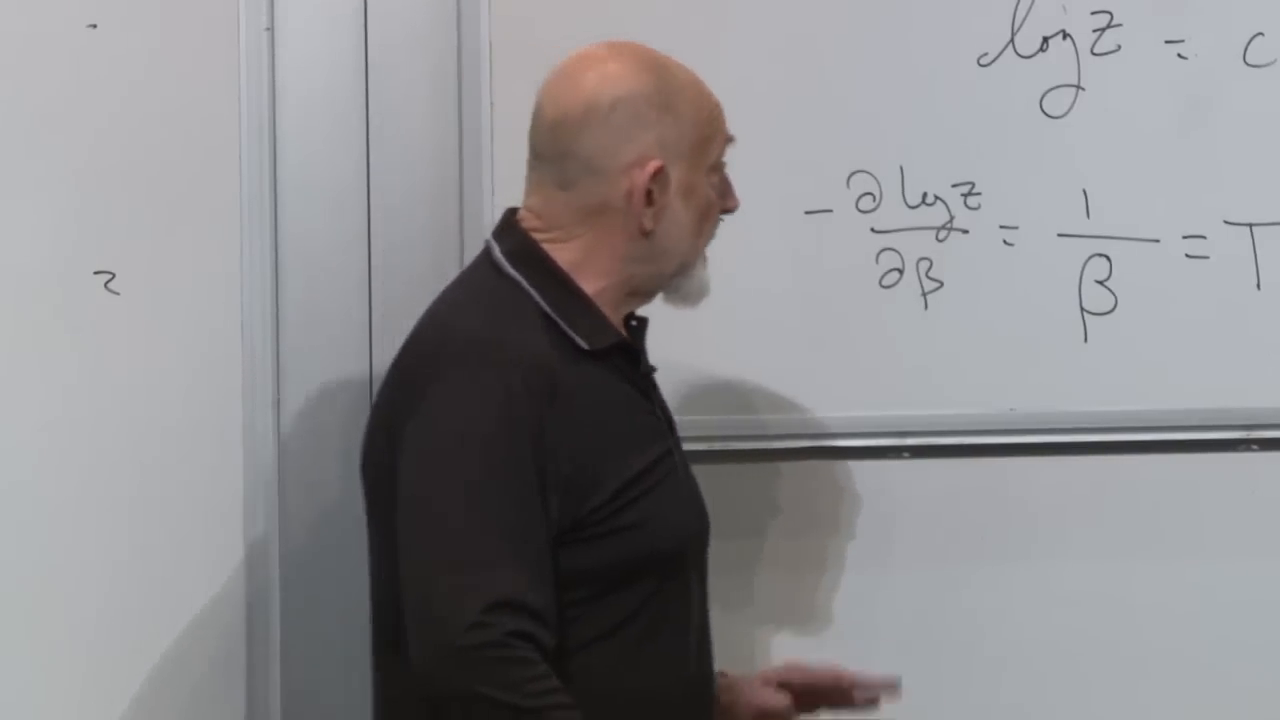
\includegraphics[width=0.90\textwidth]{lecture_07_figure_02.png}\caption{La estimación de la velocidad molecular, la derivada de la presión y la sustitución para un gas ideal, mostradas juntas.}\lectureframe{00:08:55}\end{figure}

Hay una importante precisión que hacer. Una onda sonora de pequeña amplitud suele comprimir y enrarecer el gas más rápido de lo que el calor puede fluir entre elementos vecinos. Por tanto, el movimiento local es aproximadamente adiabático, no isotérmico: \begin{equation}
 c_s^2=
 \left(\frac{\partial P}{\partial\rho_m}\right)_S.
 \label{eq:sm7-sound-adiabatic}
\end{equation}Para un gas ideal con índice adiabático \(\gamma\), \begin{equation}
 P\rho_m^{-\gamma}=\text{constant},
 \qquad
 c_s^2=\gamma\frac{P}{\rho_m}
       =\gamma\frac{k_B T}{m}.
 \label{eq:sm7-sound-ideal-adiabatic}
\end{equation}Para el aire diatómico a temperatura ambiente, \(\gamma\simeq 7/5\). Así, el cálculo a temperatura fija es una primera estimación útil, mientras que la derivada adiabática proporciona la corrección físicamente adecuada.

Con los valores aproximados \begin{equation}
\begin{aligned}
 k_B&\simeq1.3\times10^{-23}\ {\rm J\,K^{-1}},
 &T&\simeq300\ {\rm K},\\
 m_{\rm air}&\simeq4\times10^{-26}\ {\rm kg}.&&
\end{aligned}
 \label{eq:sm7-air-data}
\end{equation}la estimación molecular es de alrededor de \(500\ {\rm m\,s^{-1}}\). Aquí la temperatura debe ser una temperatura absoluta en kelvin, no una escala desplazada como la Fahrenheit. La velocidad del sonido habitual es del orden de \(300\ {\rm m\,s^{-1}}\), y la fórmula adiabática para un gas ideal da aproximadamente \(340\ {\rm m\,s^{-1}}\) a temperatura ambiente. Por tanto, el cálculo aproximado ha encontrado la escala física correcta.

\begin{figure}[t]\centering
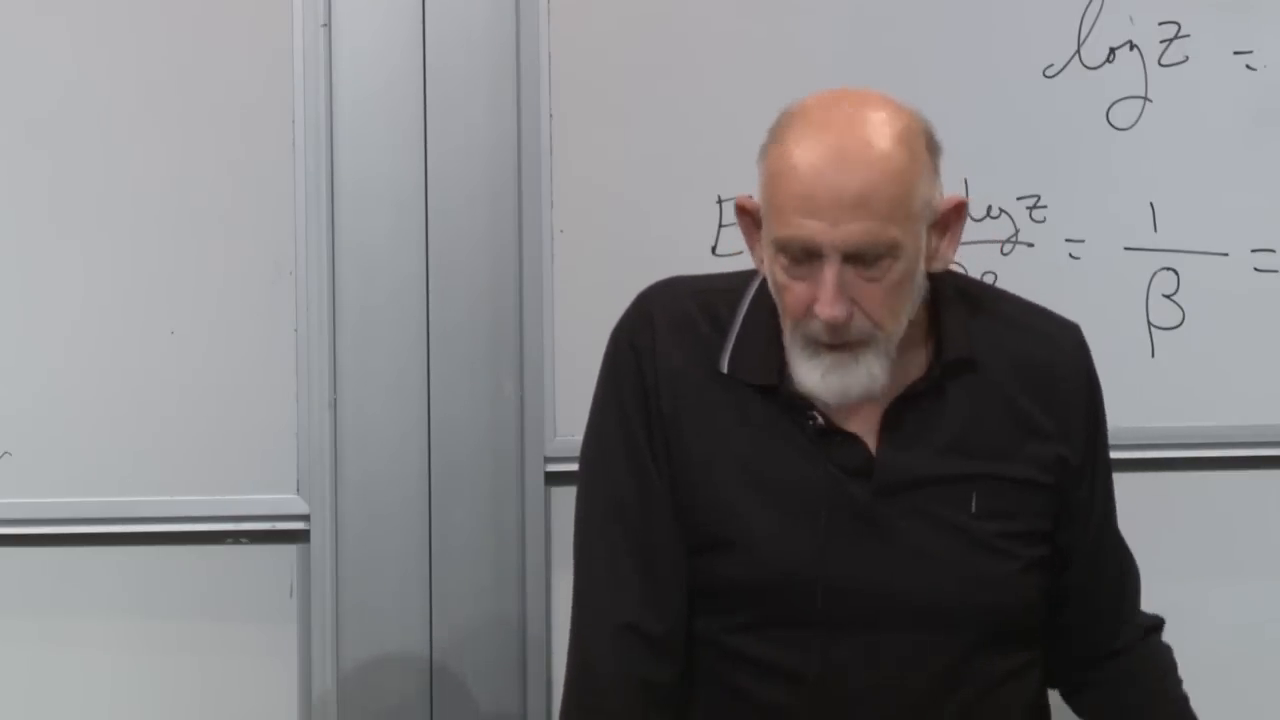
\includegraphics[width=0.90\textwidth]{lecture_07_figure_03.png}\caption{La estimación para el aire a temperatura ambiente usando la constante de Boltzmann, una masa molecular efectiva cercana a \(30\) masas de protón y \(T\simeq300\ {\rm K}\).}\lectureframe{00:10:55}\end{figure}

Mucho antes de que se dispusiera de una descripción microscópica, era posible determinar la velocidad del sonido midiendo la presión en función de la densidad. El argumento estadístico añade la sorprendente interpretación de que la velocidad macroscópica resultante está determinada por la velocidad térmica de las moléculas individuales.

\begin{classroomqa}\audiencequestion{¿Hay que añadir los neutrones a la masa molecular? ¿El número \(14\) del nitrógeno cuenta solo los protones?}\lecturerresponse{El peso atómico citado ya cuenta los protones y los neutrones. El nitrógeno molecular contiene dos átomos de peso atómico cercano a \(14\), así que su masa es de aproximadamente \(28\) masas de protón; para esta estimación basta redondear \(28\) a \(30\).\lecturetimestamp{00:10:58--00:11:16}}\end{classroomqa}

\begin{classroomqa}\audiencequestion{El factor \(3\) proviene de las tres direcciones de traslación, mientras que el sonido se propaga en una sola dirección. ¿Debería esto eliminar el factor \(3\)?}\lecturerresponse{Esto nos advierte correctamente que no debemos identificar la velocidad cuadrática media tridimensional de las moléculas con una velocidad de propagación unidimensional. El argumento inicial solo ofrecía una imagen de orden de magnitud. Una respuesta controlada se obtiene a partir de la derivada de la presión, junto con la condición termodinámica adecuada para la onda.\lecturetimestamp{00:11:12--00:12:00}}\end{classroomqa}

\begin{classroomqa}\audiencequestion{¿La derivada suponía que la temperatura permanece constante durante la onda?}\lecturerresponse{La sustitución para un gas ideal que se muestra sí lo suponía. Mantener fija la temperatura es una estimación provisional plausible para una perturbación muy pequeña; la corrección habitual es que el sonido ordinario es aproximadamente adiabático, lo que sustituye la derivada isotérmica por \(\left(\partial P/\partial\rho_m\right)_S\).\lecturetimestamp{00:12:59--00:14:01}}\end{classroomqa}

\begin{classroomqa}\audiencequestion{Si las variaciones de presión y densidad son ambas pequeñas, ¿su derivada también es pequeña?}\lecturerresponse{No. Una derivada es el cociente de dos variaciones pequeñas en el límite infinitesimal. Tanto \(\delta P\) como \(\delta\rho\) pueden ser pequeñas, mientras que \(\delta P/\delta\rho\) permanece finito y determina la velocidad de la onda.\lecturetimestamp{00:14:03--00:14:23}}\end{classroomqa}

\begin{classroomqa}\audiencequestion{¿Debería aumentar la velocidad del sonido al comprimir el gas, como ocurre al pasar de un gas a un líquido o un sólido?}\lecturerresponse{Sí. La derivada se evalúa en el estado considerado, y \(P(\rho,T)\) no tiene por qué seguir siendo lineal. Cuando las moléculas se comprimen y quedan muy juntas, la ecuación de estado deja de ser ideal y \(\partial P/\partial\rho\) puede crecer considerablemente.\lecturetimestamp{00:14:25--00:15:13}}\end{classroomqa}

\begin{classroomqa}\audiencequestion{¿Puede usarse el valor \(500\ {\rm m\,s^{-1}}\) a cualquier presión?}\lecturerresponse{No. Corresponde al intervalo de baja densidad en el que la ecuación del gas ideal es una aproximación útil. Cuando aparecen potencias superiores de la densidad en \(P(\rho,T)\), la derivada y, por tanto, la velocidad del sonido dependen de la presión y de la densidad.\lecturetimestamp{00:15:14--00:16:29}}\end{classroomqa}

\begin{classroomqa}\audiencequestion{¿También deja de ser válida, al aumentar la densidad, la imagen inicial del sonido propagándose aproximadamente a la velocidad molecular?}\lecturerresponse{Probablemente. Esa imagen está pensada para un gas diluido. Las interacciones colectivas cobran cada vez más importancia a densidad alta, precisamente por lo cual la derivada de la ecuación de estado es una descripción más general.\lecturetimestamp{00:16:32--00:16:53}}\end{classroomqa}

\begin{classroomqa}\audiencequestion{¿Por qué se escribió que la masa de una molécula de nitrógeno es aproximadamente \(30\) masas de protón y no \(28\)?}\lecturerresponse{Solo se necesita la precisión numérica apropiada para la estimación, así que \(28\) se redondeó a \(30\). Dividir también la estimación original de \(500\ {\rm m\,s^{-1}}\) entre \(\sqrt{3}\simeq1.7\) la aproxima a \(300\ {\rm m\,s^{-1}}\), aunque la derivada adiabática es la forma controlada de calcular la corrección.\lecturetimestamp{00:16:54--00:17:27}}\end{classroomqa}

\section{Un oscilador clásico en un baño térmico}

Ahora sustituimos la molécula que se traslada libremente por un oscilador armónico y tratamos todo lo demás como un baño térmico. La imagen inmediata es una masa unida a un resorte, pero el modelo es mucho más amplio. Un modo de una cavidad electromagnética oscila; los átomos de un cristal oscilan; casi cualquier sistema estable desplazado ligeramente del equilibrio ejecuta un movimiento armónico en primera aproximación.

Con \(x\) medido desde el equilibrio, el momento \(p\), la masa \(m\) y la constante del resorte \(\kappa\), el hamiltoniano es \begin{equation}
 H(x,p)=\frac{p^2}{2m}+\frac{\kappa x^2}{2},
 \qquad
 \omega=\sqrt{\frac{\kappa}{m}}.
 \label{eq:sm7-classical-hamiltonian}
\end{equation}El baño fija \(T\) y, a partir de aquí, volvemos a usar \(k_B=1\), de modo que \(\beta=1/T\). Un oscilador en equilibrio con el ambiente tiene una temperatura cercana a \(300\ {\rm K}\); uno sumergido en helio líquido tiene una temperatura de apenas unos kelvin. Un resorte hipotético colocado en el centro del Sol no sobreviviría como resorte, pero el ejemplo aclara el papel del entorno. El factor de Boltzmann se factoriza: \begin{equation}
 e^{-\beta H}
 =e^{-\beta p^2/(2m)}
  e^{-\beta\kappa x^2/2}.
 \label{eq:sm7-factorized-weight}
\end{equation}

\begin{figure}[t]\centering
\includegraphics[width=0.90\textwidth]{lecture_07_figure_04.png}\caption{Un oscilador de masa y resorte, y su hamiltoniano como suma de energía cinética y potencial.}\lectureframe{00:20:55}\end{figure}

A diferencia del gas libre, la integral sobre la posición no da simplemente el volumen del recipiente. El potencial restaurador pondera cada desplazamiento: \begin{equation}
 Z_{\rm cl}
 =\frac{1}{h}\int_{-\infty}^{\infty}dp
             \int_{-\infty}^{\infty}dx\,
 e^{-\beta p^2/(2m)}
 e^{-\beta\kappa x^2/2}.
 \label{eq:sm7-classical-z}
\end{equation}El factor \(1/h\) hace adimensional la función de partición clásica unidimensional. Se omite en el cálculo de la pizarra porque es independiente de \(\beta\) y no puede afectar a la energía media.

\begin{figure}[t]\centering
\includegraphics[width=0.90\textwidth]{lecture_07_figure_05.png}\caption{La función de partición clásica del oscilador, separada en sus integrales gaussianas sobre el momento y el desplazamiento.}\lectureframe{00:22:55}\end{figure}

Para la integral sobre el momento, hacemos el cambio de variable \begin{equation}
 q=\sqrt{\frac{\beta}{2m}}\,p,
 \qquad
 dp=\sqrt{\frac{2m}{\beta}}\,dq.
 \label{eq:sm7-p-gaussian-substitution}
\end{equation}Para la integral sobre la posición, hacemos el cambio de variable \begin{equation}
 y=\sqrt{\frac{\beta\kappa}{2}}\,x,
 \qquad
 dx=\sqrt{\frac{2}{\beta\kappa}}\,dy.
 \label{eq:sm7-x-gaussian-substitution}
\end{equation}Como \(\int_{-\infty}^{\infty}e^{-u^2}\,du=\sqrt{\pi}\), la integral no normalizada sobre el espacio de fases usada en la pizarra es \begin{equation}
 \int dp\,dx\,e^{-\beta H}
 =\frac{2\pi}{\beta}\sqrt{\frac{m}{\kappa}}
 =\frac{2\pi}{\beta\omega}.
 \label{eq:sm7-classical-z-unnormalized}
\end{equation}Al restituir la celda del espacio de fases, \begin{equation}
 Z_{\rm cl}=\frac{2\pi}{h\beta\omega}
           =\frac{1}{\beta\hbar\omega}.
 \label{eq:sm7-classical-z-normalized}
\end{equation}

Para la energía solo importa la dependencia de \(\beta\): \begin{equation}
 \begin{aligned}
 \log Z_{\rm cl}&=\text{constant}-\log\beta,\\
 \expect{H}
 &=-\frac{\partial\log Z_{\rm cl}}{\partial\beta}\\
 &=\frac{1}{\beta}=T.
 \end{aligned}
 \label{eq:sm7-classical-energy}
\end{equation}

\begin{figure}[t]\centering
\includegraphics[width=0.90\textwidth]{lecture_07_figure_06.png}\caption{La cadena clásica completa en la pizarra de la derecha: factorización gaussiana, \(Z\propto(\beta\omega)^{-1}\) y \(\expect{H}=1/\beta=T\).}\lectureframe{00:30:15}\end{figure}

No aparece ningún factor de \(3\) porque se trata de un oscilador espacial. Tampoco queda ningún factor de \(1/2\), porque hay dos términos cuadráticos independientes. Cada gaussiana aporta \(T/2\): \begin{equation}
 \expect{K}=\frac{T}{2},
 \qquad
 \expect{U}=\frac{T}{2},
 \qquad
 \expect{H}=T.
 \label{eq:sm7-equipartition-oscillator}
\end{equation}Esta es la equipartición en su forma más útil: cada término cuadrático independiente del hamiltoniano clásico aporta \(T/2\).

La respuesta es independiente tanto de \(m\) como de \(\kappa\). El movimiento sí depende de esos parámetros: \begin{equation}
 \expect{p^2}=mT,
 \qquad
 \expect{x^2}=\frac{T}{\kappa},
 \qquad
 \expect{\dot{x}^2}=\frac{T}{m}.
 \label{eq:sm7-classical-fluctuations}
\end{equation}Así, una masa mayor se mueve más despacio y un resorte más rígido tiene una amplitud menor, aunque la energía media siga siendo \(T\). Esto resulta inquietante cuando \(\kappa\) se hace descomunalmente grande. Un resorte tan rígido que no pueda moverse debería parecer una restricción congelada; sin embargo, la equipartición clásica todavía le asigna una energía \(T\).

\begin{classroomqa}\audiencequestion{Cuando \(\kappa\to\infty\), la función de partición tiende a cero. ¿Cómo puede seguir usándose su logaritmo?}\lecturerresponse{Mantengamos \(\kappa\) finita, pero arbitrariamente grande. Su contribución a \(\log Z\) es aditiva e independiente de \(\beta\), así que la derivada respecto de \(\beta\) sigue dando \(T\). La inquietud en el límite es real: el cálculo clásico es internamente coherente, pero omite una característica de la naturaleza necesaria para los osciladores muy rígidos.\lecturetimestamp{00:34:01--00:34:54}}\end{classroomqa}

\begin{classroomqa}\audiencequestion{La función de partición del gas ideal requería un \(N!\). ¿Debería aparecer aquí un factorial análogo?}\lecturerresponse{No. Estudiamos un oscilador especificado, no permutamos \(N\) partículas idénticas. Para muchos modos independientes etiquetados, las funciones de partición se multiplican. El factor de indistinguibilidad corresponde a un problema de conteo distinto.\lecturetimestamp{00:35:03--00:35:40}}\end{classroomqa}

\section{Por qué la equipartición clásica fue una crisis}

Las moléculas reales no son puntos sin estructura. Una molécula diatómica contiene un enlace que puede vibrar, es decir, un oscilador interno. Un conteo clásico ingenuo asignaría a ese modo energía térmica adicional incluso a temperaturas ordinarias. En un conteo deliberadamente esquemático, activar un oscilador vibratorio eleva una energía de \(3T/2\) a un valor cercano a \(5T/2\). Un cálculo preciso del calor específico también debe incluir los grados de libertad rotacionales y distinguir la energía de su derivada respecto de la temperatura. El hecho experimental decisivo es más sencillo: los modos internos rígidos no contribuían a baja temperatura, pese a lo que exigía la equipartición clásica.

Se podría negar que la molécula tenga estructura interna, lo cual es absurdo, o reconocer que a la mecánica clásica le falta un ingrediente. Ese ingrediente es la mecánica cuántica. Necesitamos muy poco de ella: solo que un oscilador armónico tiene niveles de energía equiespaciados.

\section{El oscilador cuántico}

Primero desplazamos el origen de energía y escribimos el espectro de excitación como \begin{equation}
 E_n^{\rm exc}=n\hbar\omega,
 \qquad n=0,1,2,\ldots.
 \label{eq:sm7-shifted-spectrum}
\end{equation}Ahora la función de partición es una suma genuina, en lugar de una integral sobre el espacio de fases: \begin{align}
 Z_{\rm exc}
 &=\sum_{n=0}^{\infty}e^{-\beta n\hbar\omega} \notag\\
 &=1+x+x^2+\cdots
  =\frac{1}{1-x},
 \qquad x=e^{-\beta\hbar\omega}, \notag\\
 &=\frac{1}{1-e^{-\beta\hbar\omega}}.
 \label{eq:sm7-quantum-z}
\end{align}

\begin{figure}[t]\centering
\includegraphics[width=0.90\textwidth]{lecture_07_figure_07.png}\caption{Niveles equiespaciados y evaluación de la serie geométrica para la función de partición del oscilador cuántico.}\lectureframe{00:42:05}\end{figure}

Al derivar, obtenemos la energía media de excitación: \begin{align}
 E_{\rm exc}
 &=-\frac{\partial\log Z_{\rm exc}}{\partial\beta}
  =-\frac{1}{Z_{\rm exc}}
    \frac{\partial Z_{\rm exc}}{\partial\beta}
 \notag\\
 &=\hbar\omega\,
   \frac{e^{-\beta\hbar\omega}}
        {1-e^{-\beta\hbar\omega}}
  =\frac{\hbar\omega}{e^{\beta\hbar\omega}-1}.
 \label{eq:sm7-quantum-energy}
\end{align}

\begin{figure}[t]\centering
\includegraphics[width=0.90\textwidth]{lecture_07_figure_08.png}\caption{La energía de excitación térmica obtenida mediante la derivada respecto de \(\beta\) de la función de partición cuántica.}\lectureframe{00:46:05}\end{figure}

\subsection{Temperatura alta}

Cuando \(\beta\hbar\omega\ll1\), \begin{equation}
 e^{-\beta\hbar\omega}
 =1-\beta\hbar\omega
  +O\!\left((\beta\hbar\omega)^2\right).
 \label{eq:sm7-high-t-expansion}
\end{equation}El numerador de \eqref{eq:sm7-quantum-energy} se aproxima a \(\hbar\omega\), mientras que el denominador es \(\beta\hbar\omega\) en orden dominante. Por tanto, \begin{equation}
 E_{\rm exc}\simeq\frac{1}{\beta}=T.
 \label{eq:sm7-high-t-energy}
\end{equation}La respuesta cuántica recupera la equipartición clásica cuando caben muchos intervalos entre niveles dentro de la energía térmica.

\subsection{Temperatura baja}

Cuando \(\beta\hbar\omega\gg1\), la exponencial es muy pequeña: \begin{equation}
 E_{\rm exc}
 \simeq\hbar\omega e^{-\beta\hbar\omega}.
 \label{eq:sm7-low-t-energy}
\end{equation}La excitación térmica del oscilador está suprimida exponencialmente. En la convención desplazada es casi nula; más adelante restituiremos la energía física de punto cero.

\begin{figure}[t]\centering
\includegraphics[width=0.90\textwidth]{lecture_07_figure_09.png}\caption{La expansión a baja temperatura: la primera excitación térmica está suprimida por \(e^{-\beta\hbar\omega}\).}\lectureframe{00:51:55}\end{figure}

La transición ocurre cuando \begin{equation}
 \beta\hbar\omega\sim1,
 \qquad\text{or equivalently}\qquad
 T\sim\hbar\omega.
 \label{eq:sm7-crossover}
\end{equation}Esta condición tiene un significado directo. La equipartición clásica asignaría al oscilador una energía \(T\). Los efectos cuánticos se vuelven inevitables cuando esa escala cae por debajo de un intervalo entre niveles. Así, \begin{equation}
\begin{aligned}
 \hbar\omega\gg T&:\quad \text{frozen and quantum},\\
 \hbar\omega\ll T&:\quad \text{active and classical}.
\end{aligned}
 \label{eq:sm7-regimes}
\end{equation}Un resorte más rígido tiene un \(\omega=\sqrt{\kappa/m}\) mayor, por lo que hace falta una temperatura más alta para que se comporte clásicamente.

\section{Los grados de libertad aparecen al calentar la materia}

A baja temperatura, una molécula diatómica puede comportarse térmicamente como una partícula puntual porque la vibración de su enlace rígido está congelada. A medida que \(T\) aumenta y supera \(\hbar\omega\), se activa el modo vibratorio. Los modos rotacionales pueden activarse a una escala más baja; a temperaturas aún mayores se hacen visibles otros movimientos internos y, finalmente, el átomo se ioniza. Calentar no solo aporta más energía a una lista fija de modos: revela grados de libertad que eran invisibles a temperaturas más bajas.

Una molécula anidada imaginaria permite precisar la idea. Dos átomos están unidos por un resorte rígido, mientras que uno de los átomos aparentes es, a su vez, un par unido por un resorte aún más rígido. A baja \(T\), ambas estructuras parecen puntuales. Al alcanzar el primer umbral aparece la vibración exterior; al llegar al segundo, aparece la estructura interior. La complejidad del sistema se descubre escala de energía a escala de energía.

\begin{classroomqa}\audiencequestion{Una vez que el oscilador ya está en el régimen clásico, ¿calentarlo más tensa el resorte o cambia su frecuencia?}\lecturerresponse{No. La constante del resorte y la frecuencia permanecen fijas. Una temperatura más alta produce momentos y amplitudes típicos mayores y, por tanto, más energía. La rigidez determina la temperatura a la que comienza a regir la ley clásica, no un aumento de la tensión del resorte dependiente de la temperatura.\lecturetimestamp{01:03:17--01:05:11}}\end{classroomqa}

\subsection{Cristales y el calor específico de Einstein}

Un cristal contiene muchísimos modos vibratorios. La equipartición clásica asigna una energía del orden de \(T\) a cada oscilador activo y, por tanto, sobreestima el calor específico a baja temperatura. El modelo de Einstein de 1907 trató cuánticamente las vibraciones del cristal y mostró por qué quedan suprimidas hasta que la energía térmica alcanza el intervalo entre niveles. Los modelos más precisos de la física del estado sólido admiten una distribución de frecuencias de los modos, pero el principio de congelación ya está presente en el cálculo de Einstein.

\begin{classroomqa}\audiencequestion{¿Fue este el trabajo por el que Einstein recibió el Premio Nobel? ¿Se publicó solo después de que se estableciera la mecánica cuántica?}\lecturerresponse{No. La mención del Nobel se refería al efecto fotoeléctrico. El modelo del calor específico se publicó en 1907, mucho antes de que se comprendieran los fundamentos completos de la mecánica cuántica. Einstein aceptó y desarrolló ideas cuánticas fundamentales, aunque más tarde objetara algunos aspectos de la teoría madura.\lecturetimestamp{00:58:38--01:03:16}}\end{classroomqa}

\begin{classroomqa}\audiencequestion{La mecánica estadística clásica sustituyó una suma sobre estados discretos por una integral aparentemente uniforme sobre la posición y el momento. ¿Qué justifica ese conteo de estados?}\lecturerresponse{La justificación última proviene de la mecánica cuántica. En el límite de alta temperatura, \[
 Z_{\rm exc}\simeq\frac{1}{\beta\hbar\omega},
\]lo que coincide exactamente con el resultado clásico adimensional \eqref{eq:sm7-classical-z-normalized}. Las celdas cuánticas del espacio de fases se convierten en la medida clásica de ese espacio cuando no se resuelven los intervalos entre niveles.\lecturetimestamp{00:59:38--01:03:06}}\end{classroomqa}

\subsection{Una cuerda contiene infinitos osciladores}

Una cuerda de violín o de guitarra se descompone en modos normales: el fundamental, los armónicos superiores y longitudes de onda cada vez más cortas. Matemáticamente, hay infinitos modos oscilatorios. Si la equipartición clásica asignara energía \(T\) a cada uno, la cuerda en equilibrio térmico tendría energía infinita. La mecánica cuántica evita esa catástrofe. Los modos de longitud de onda más corta tienen las frecuencias más altas y permanecen congelados a cualquier temperatura finita; a medida que \(T\) aumenta, se activan progresivamente más modos. La misma idea fundamentará más adelante la radiación de cuerpo negro.

\begin{figure}[t]\centering
\includegraphics[width=0.90\textwidth]{lecture_07_figure_10.png}\caption{Varios modos normales superpuestos en una cuerda, que ilustran por qué una cuerda continua equivale a una colección infinita de osciladores armónicos.}\lectureframe{01:09:30}\end{figure}

\begin{classroomqa}\audiencequestion{¿Puede observarse directamente la transición de lo cuántico a lo clásico? ¿Puede el calentamiento invertir el comportamiento de baja temperatura?}\lecturerresponse{Sí. La dependencia con la temperatura del calor específico de un cristal permite medir claramente la congelación y la posterior activación de los modos vibratorios.\lecturetimestamp{01:09:11--01:10:13}}\end{classroomqa}

\begin{classroomqa}\audiencequestion{Para muchos osciladores, ¿repetimos la función de partición de un solo oscilador para cada modo?}\lecturerresponse{Para modos independientes, \[
\begin{aligned}
 Z_{\rm tot}&=\prod_j Z_j,&
 \log Z_{\rm tot}&=\sum_j\log Z_j,\\
 E_{\rm tot}&=\sum_j E_j.&&
\end{aligned}
\]Los modos con \(\hbar\omega_j\gg T\) hacen contribuciones térmicas exponencialmente pequeñas; los que están por debajo del umbral contribuyen de forma apreciable.\lecturetimestamp{01:10:14--01:11:00}}\end{classroomqa}

\begin{classroomqa}\audiencequestion{¿Qué ocurrió con la energía de punto cero del oscilador, \(\hbar\omega/2\)?}\lecturerresponse{Los niveles físicos son \[
 E_n=\left(n+\frac12\right)\hbar\omega.
\]Por consiguiente, \[
 \begin{aligned}
 Z_{\rm phys}
 &=e^{-\beta\hbar\omega/2}Z_{\rm exc},\\
 E_{\rm phys}
 &=\frac{\hbar\omega}{2}
  +\frac{\hbar\omega}{e^{\beta\hbar\omega}-1}.
 \end{aligned}
\]El desplazamiento común no cambia las probabilidades de los niveles, la entropía, el calor específico ni la energía de excitación térmica, pero sí desplaza la energía media absoluta en \(\hbar\omega/2\). El factor multiplicativo en \(Z\) depende de \(\beta\), así que no debe descartarse cuando se busca la energía absoluta.\lecturetimestamp{01:11:08--01:11:37}}\end{classroomqa}

\section{La segunda ley como enigma de la reversibilidad}

Ahora podemos volver al problema anunciado. La segunda ley afirma que la evolución macroscópica ordinaria es irreversible y que la entropía tiende a aumentar. La evolución hamiltoniana microscópica es reversible. ¿Cómo puede una transformación reversible de estados exactos producir una ley irreversible para estados macroscópicos?

Representemos el sistema mediante un punto en un espacio de fases de alta dimensión, \[
 \Gamma=(q_1,\ldots,q_N,p_1,\ldots,p_N).
\]Por lo general, nuestro conocimiento no corresponde a un punto exacto. Supongamos que consiste en una densidad de probabilidad uniforme en una región compacta \(A\) de volumen \(\Omega_A\): \begin{equation}
 f(\Gamma)=
 \begin{cases}
  1/\Omega_A,&\Gamma\in A,\\
  0,&\Gamma\notin A.
 \end{cases}
 \label{eq:sm7-uniform-blob}
\end{equation}En unidades con \(k_B=1\), su entropía de Gibbs fina es \begin{equation}
 S_{\rm fine}
 =-\int d\Gamma\,f\log f
 =\log\Omega_A.
 \label{eq:sm7-blob-entropy}
\end{equation}Una región más pequeña implica más información y menor entropía. Esto fija el signo: al aumentar la incertidumbre, crece la región ocupada y aumenta \(\log\Omega_A\).

\begin{figure}[t]\centering
\includegraphics[width=0.90\textwidth]{lecture_07_figure_11.png}\caption{Una región compacta de probabilidad en una sección esquemática bidimensional del espacio de fases completo de posiciones y momentos.}\lectureframe{01:20:20}\end{figure}

\begin{classroomqa}\audiencequestion{¿El sistema está físicamente restringido a permanecer dentro de la región dibujada? ¿Ya está en equilibrio?}\lecturerresponse{No. La región describe lo que se sabe sobre el estado inicial, no una pared en el espacio de fases. No tiene por qué ser una distribución de equilibrio. Un gas confinado inicialmente en un tanque situado en una esquina de una habitación es un ejemplo concreto de información especial, fuera del equilibrio.\lecturetimestamp{01:14:55--01:15:24}}\end{classroomqa}

\section{Flujo de Liouville y crecimiento por coarse-graining}

El teorema de Liouville afirma que el flujo hamiltoniano conserva el volumen del espacio de fases. La región exacta puede trasladarse, estirarse, plegarse y volverse extremadamente delgada, pero \begin{equation}
 \Omega_{A(t)}=\Omega_{A(0)},
 \qquad
 S_{\rm fine}(t)=S_{\rm fine}(0).
 \label{eq:sm7-liouville}
\end{equation}El análogo discreto es una permutación reversible de estados. Si al principio sabemos que un dado está en uno de dos estados, una evolución biyectiva puede cambiar cuáles son esos dos estados, pero no cambia el número de posibilidades.

Las descripciones reales tienen una resolución finita. La mecánica cuántica proporciona una celda natural en el espacio de fases, mientras que un experimento clásico también tiene una capacidad de medición finita, incluso sin invocar la teoría cuántica. Bajo el flujo hamiltoniano, la región puede convertirse en una serpiente larga y delgada. Si la separación entre pliegues vecinos cae por debajo de la escala de resolución, sustituimos cada vecindad que no podemos resolver por una celda gruesa. El volumen exacto ocupado permanece constante, pero la unión de las celdas gruesas crece: \begin{equation}
 \Omega_{\rm coarse}(t)\geq\Omega_{A(t)},
 \qquad
 S_{\rm coarse}(t)=\log\Omega_{\rm coarse}(t).
 \label{eq:sm7-coarse-entropy}
\end{equation}

\begin{figure}[t]\centering
\includegraphics[width=0.90\textwidth]{lecture_07_figure_12.png}\caption{Un filamento que conserva el volumen, observado con celdas de resolución finita. El filamento negro exacto conserva su área; las celdas gruesas rojas ocupan una región efectiva mayor.}\lectureframe{01:22:10}\end{figure}

\begin{classroomqa}\audiencequestion{Las celdas gruesas se solapan. ¿Viola eso el teorema de Liouville?}\lecturerresponse{No. Liouville rige el filamento exacto, que sigue siendo biyectivo y conserva el volumen. El solapamiento pertenece a nuestra descripción borrosa: hemos descartado la información sobre cuál de las hebras delgadas contiene el estado.\lecturetimestamp{01:21:32--01:21:50}}\end{classroomqa}

Una analogía útil es el algodón. El volumen material de todas las fibras puede permanecer casi constante mientras que un montón deshilachado ocupa un gran volumen aparente para un observador incapaz de resolver las fibras individuales. De igual modo, una región del espacio de fases desarrolla tentáculos cada vez más finos, y estos, a su vez, desarrollan otros aún más finos. Toda resolución finita fija acaba por no poder seguirlos.

\begin{classroomqa}\audiencequestion{¿La entropía solo parece aumentar en la descripción clásica, mientras que la mecánica cuántica hace real el aumento al imponer un límite fundamental de resolución?}\lecturerresponse{El argumento del coarse-graining no requiere un límite cuántico. La entropía se refiere conjuntamente al sistema y a las distinciones macroscópicas que conserva su descripción. Con información microscópica infinita, la entropía fina es constante; con cualquier resolución finita fija, los filamentos caóticos acaban por volverse irresolubles y la entropía gruesa aumenta.\lecturetimestamp{01:24:04--01:25:20}}\end{classroomqa}

\section{Caos, una región accesible finita y la equilibración}

En un gas dentro de una caja, las posiciones están acotadas. A energía total finita fija, los momentos también están acotados, aunque toda la energía se concentre momentáneamente en una sola partícula. Por tanto, bajo las hipótesis habituales de confinamiento, la superficie de energía dinámicamente accesible tiene medida finita.

\begin{figure}[t]\centering
\includegraphics[width=0.90\textwidth]{lecture_07_figure_13.png}\caption{Una región acotada del espacio de fases accesible junto al filamento y su representación por coarse-graining.}\lectureframe{01:28:10}\end{figure}

Los puntos iniciales cercanos de un sistema caótico siguen historias similares durante un tiempo y luego se separan. En una partida de billar, un cambio imperceptible en la dirección de la bola blanca se transmite a las colisiones posteriores; las diferencias se acumulan hasta que las configuraciones finales dejan de guardar relación entre sí. Por tanto, una región inicial completa se estira y se pliega por toda la región accesible. A resolución finita, se aproxima a una descripción de equilibrio amplia y casi uniforme.

\begin{figure}[t]
\centering
\includegraphics[width=0.90\textwidth]{lecture_07_figure_14.png}
\caption{Un estado especial compacto evoluciona hasta convertirse en un filamento complejo que se extiende por la región accesible acotada, mientras las celdas de grano grueso se dispersan por un área mucho mayor.}
\lectureframe{01:33:10}
\end{figure}

Hay que tener en cuenta dos matices. El caos, por sí solo, no demuestra que toda trayectoria visite cada entorno accesible; esa afirmación más fuerte sobre el muestreo requiere una propiedad ergódica o de mezcla. Tampoco todos los sistemas físicos son caóticos. Un gas genérico de muchas partículas y los billares idealizados son ejemplos del contexto previsto, en el que la mezcla constituye una expectativa física razonable.

\section{La recurrencia no elimina la irreversibilidad}

Supongamos que todas las moléculas de aire comienzan en un rincón con un patrón de velocidades preparado especialmente. Las colisiones las dispersan rápidamente por la habitación y la descripción de grano grueso alcanza el equilibrio. En un espacio de fases finito que conserva la medida, el teorema de recurrencia de Poincaré afirma que casi todo punto inicial vuelve a estar arbitrariamente cerca de su punto de partida. Para una tolerancia \(\epsilon>0\), el tiempo de recurrencia \(t_R(\epsilon)\) es finito si se cumplen las hipótesis del teorema, aunque para un sistema macroscópico es extraordinariamente grande. No se requiere ni suele esperarse un retorno exacto a un punto con precisión infinita.

\begin{classroomqa}
\audiencequestion{En el ejemplo del billar, ¿golpear la bola blanca aporta energía y arruina la evolución del sistema cerrado?}
\lecturerresponse{El estado inicial elegido comienza justo después del golpe, con esa energía ya incluida. La recurrencia se refiere a la dinámica subsiguiente del billar idealizado y aislado; un retorno cercano al estado inicial incluye una configuración equivalente a la aproximación de la bola blanca al triángulo de bolas dentro de la tolerancia elegida.
\lecturetimestamp{01:35:37--01:35:55}}
\end{classroomqa}

\begin{classroomqa}
\audiencequestion{Si el gas puede volver al rincón con el tiempo, ¿hemos perdido información y es realmente reversible el sistema?}
\lecturerresponse{La dinámica microscópica sigue siendo reversible en todo momento. La entropía de grano grueso puede aumentar porque dejamos de resolver las correlaciones finas; sin embargo, una fluctuación excepcionalmente rara puede devolver el sistema a un estado cercano a su macroestado inicial especial. Por tanto, la recurrencia y la irreversibilidad de grano grueso son compatibles.
\lecturetimestamp{01:37:34--01:38:15}}
\end{classroomqa}

Esto conduce a la formulación esencial de Boltzmann. La entropía no aumenta en todo instante lógicamente posible. Dado un macroestado de no equilibrio de un sistema grande, hay abrumadoramente más continuaciones microscópicas compatibles que conducen hacia macrostados de mayor entropía que hacia otros aún más especiales. La entropía \emph{probablemente} aumenta. Las fluctuaciones descendentes y las recurrencias están permitidas, pero sus probabilidades y escalas de tiempo las hacen invisibles en la experiencia macroscópica ordinaria. El problema de la reversibilidad fue una de las grandes dificultades históricas de la mecánica estadística y pesó mucho sobre Boltzmann. Esa conexión histórica no debe convertirse en una afirmación causal simplista sobre su vida.

\section{Qué significa el caos}

Para dar una definición más operativa del caos, supongamos que dos puntos iniciales del espacio de fases difieren en \(\delta\Gamma(0)\). En una dirección caótica, típicamente se cumple que
\begin{equation}
 \lVert\delta\Gamma(t)\rVert
 \sim e^{\lambda t}\lVert\delta\Gamma(0)\rVert,
 \qquad \lambda>0,
 \label{eq:sm7-lyapunov-growth}
\end{equation}
dentro del régimen en que la separación linealizada tiene sentido. El número \(\lambda\) es un exponente de Lyapunov. Para predecir durante un tiempo \(t\), la precisión requerida en los datos iniciales escala aproximadamente como \(e^{-\lambda t}\). La precisión de las leyes dinámicas también importa: los errores del modelo se amplifican junto con los errores en las condiciones iniciales. El tiempo atmosférico es el ejemplo más conocido.

\begin{classroomqa}
\audiencequestion{¿Hay algún principio que diga que \emph{la mayoría} de los sistemas son caóticos, o es algo meramente empírico?}
\lecturerresponse{Hay infinitos hamiltonianos caóticos y no caóticos, e incluso la palabra \emph{mayoría} requiere definir una medida en el espacio de hamiltonianos. Los sistemas complejos con interacciones suelen ser caóticos, pero no existe una prueba universal elemental que permita clasificar a simple vista cualquier hamiltoniano.
\lecturetimestamp{01:39:27--01:40:49}}
\end{classroomqa}

\begin{classroomqa}
\audiencequestion{¿Qué significa exactamente \emph{caótico} en este contexto?}
\lecturerresponse{Las trayectorias cercanas en el espacio de fases se separan con suficiente rapidez como para que las predicciones a largo plazo requieran un conocimiento de las condiciones iniciales que mejore exponencialmente. El oscilador armónico ofrece el contraste: los puntos cercanos del espacio de fases giran juntos y permanecen próximos. El problema exacto de Kepler de dos cuerpos tampoco es caótico, mientras que el problema general de tres cuerpos tiene regímenes caóticos.
\lecturetimestamp{01:40:50--01:43:45}}
\end{classroomqa}

\begin{classroomqa}
\audiencequestion{¿Es necesario conocer con gran precisión las leyes del movimiento, además de las condiciones iniciales?}
\lecturerresponse{Sí. Ambas fuentes de error se propagan por la dinámica, y la evolución caótica amplifica las dos.
\lecturetimestamp{01:43:46--01:43:55}}
\end{classroomqa}

El péndulo doble ofrece un ejemplo muy ilustrativo. Un péndulo ordinario es integrable y predecible. Al añadir un segundo péndulo, las trayectorias que comienzan casi juntas pueden acabar transfiriendo energía de manera distinta y dirigiéndose en direcciones completamente diferentes.

\begin{figure}[t]
\centering
\includegraphics[width=0.90\textwidth]{lecture_07_figure_15.png}
\caption{El péndulo doble como ejemplo concreto de caos determinista.}
\lectureframe{01:44:40}
\end{figure}

\begin{classroomqa}
\audiencequestion{¿Por qué un sistema mecánico puede ser caótico y otro no?}
\lecturerresponse{Eso es una propiedad del hamiltoniano y de sus estructuras invariantes, no una consecuencia de la fricción ni del ruido experimental. Determinarlo puede ser matemáticamente difícil; la complejidad es un indicio, pero no una demostración.
\lecturetimestamp{01:44:03--01:45:58}}
\end{classroomqa}

\begin{classroomqa}
\audiencequestion{¿Sigue siendo caótico un péndulo doble ideal sin fricción?}
\lecturerresponse{Sí. No se requiere disipación. El movimiento hamiltoniano determinista exacto puede presentar dependencia sensible de las condiciones iniciales. Unos datos iniciales de precisión infinita determinarían la trayectoria indefinidamente, pero la precisión finita impone un horizonte de predicción finito.
\lecturetimestamp{01:45:57--01:47:54}}
\end{classroomqa}

\begin{classroomqa}
\audiencequestion{¿Es lo mismo el caos que no tener una solución de forma cerrada?}
\lecturerresponse{No. Por lo general, los sistemas caóticos carecen de una trayectoria de forma cerrada que resulte útil globalmente, pero la resolubilidad analítica y la dependencia sensible son propiedades distintas. El caos se diagnostica dinámicamente por la separación de trayectorias, no simplemente por nuestra incapacidad para escribir una fórmula.
\lecturetimestamp{01:48:20--01:49:23}}
\end{classroomqa}

\begin{classroomqa}
\audiencequestion{¿En qué se diferencia un caos generalizado de mantener el equilibrio exacto en la cima inestable de una colina?}
\lecturerresponse{La cima de la colina es un estado inestable excepcional: lejos de ella, las trayectorias cercanas no tienen por qué separarse rápidamente. En una región caótica, la inestabilidad es típica a lo largo de la órbita y los puntos cercanos del espacio de fases se separan repetidamente. Un exponente de Lyapunov positivo caracteriza ese crecimiento persistente.
\lecturetimestamp{01:49:27--01:50:11}}
\end{classroomqa}

\section{Del movimiento microscópico a la ley estadística}

La estimación de la velocidad del sonido mostró cómo el movimiento térmico microscópico determina una escala macroscópica de propagación, mientras que las preguntas pusieron de manifiesto la derivada termodinámica que hay que especificar. Luego, el oscilador mostró tanto el alcance como las limitaciones de la equipartición clásica. La separación entre niveles cuánticos congela los modos rígidos, explica por qué las capacidades caloríficas cambian con la temperatura e impide que un número infinito de modos de alta frecuencia transporte una energía térmica infinita.

La misma transición desde la microfísica exacta hasta una descripción macroscópica efectiva resuelve la aparente contradicción que subyace a la segunda ley. El flujo hamiltoniano conserva el volumen exacto del espacio de fases y sigue siendo reversible. El estiramiento caótico crea correlaciones más finas de las que retiene una descripción macroscópica, por lo que crece la región ocupada de grano grueso. La recurrencia garantiza que los retornos raros no están prohibidos; la probabilidad explica por qué no definen la experiencia ordinaria. La segunda ley no es una nueva fuerza microscópica irreversible. Es la dirección estadística de la evolución, abrumadoramente fiable, para condiciones iniciales macroscópicas especiales en sistemas con un número enorme de grados de libertad.
\chapter{Recurrencia, orden fuera del equilibrio y espines de Ising}

\lectureoverview{Al liberarse el gas de una mitad de una habitación, se precipita hacia el equilibrio; sin embargo, la mecánica reversible afirma que una evolución suficientemente prolongada también debe devolverlo al estado excepcional. Estimamos ese tiempo de retorno a partir del volumen del espacio de fases, distinguimos la recurrencia del comienzo de baja entropía del universo, que sigue sin explicación, y usamos el problema resultante para hablar de cerebros de Boltzmann, historia coherente y vida sostenida por un flujo de energía. Después pasamos al orden magnético. Los espines independientes de dos estados ofrecen un ejemplo introductorio exactamente soluble: la combinatoria determina la función de partición y la magnetización es una tangente hiperbólica. Por último, las interacciones entre vecinos restauran una simetría arriba--abajo y conducen al modelo de Ising unidimensional.}

\section{Una habitación llena de aire que acaba regresando}

Empecemos con todo el aire en la mitad izquierda de una habitación. Se puede preparar este estado colocando un tabique: se evacúa la mitad derecha, se deja el aire en la izquierda y luego se retira la pared. El gas se dispersa rápidamente por la habitación y se aproxima al equilibrio térmico. La entropía aumenta. No ha ocurrido nada sorprendente.

Ahora dejemos la habitación cerrada y esperemos. Obtener un millón de caras seguidas al lanzar una moneda es un resultado extraordinariamente improbable, pero un experimento que se repita indefinidamente acaba produciendo resultados extraordinariamente improbables. La misma lógica se aplica al gas. En algún momento muy lejano, todas sus moléculas volverán a encontrarse en la mitad izquierda, o en alguna región igual de especial. Ese retorno es una recurrencia de Poincaré.

El teorema preciso requiere algo más de cuidado que esta imagen. En una región de medida finita del espacio de fases cuya dinámica conserva el volumen de dicho espacio, casi todo punto inicial vuelve arbitrariamente cerca de su punto de partida. Una afirmación macroscópica como \emph{todas las moléculas están en la mitad izquierda} es más sencilla: solo exige que la trayectoria vuelva a entrar en una región finita definida a grano grueso, no que cada coordenada molecular retorne exactamente. La pregunta práctica es cuánto tarda eso.

\subsection{Un punto de fase de alta dimensión}

Para \(N\) partículas clásicas, el espacio de fases tiene \(6N\) coordenadas:
\begin{equation}
 \Gamma=(\bm x_1,\ldots,\bm x_N;\bm p_1,\ldots,\bm p_N).
 \label{eq:sm8-phase-point}
\end{equation}
La habitación acota las posiciones. A energía total fija, los momentos también están acotados, porque ninguna partícula puede tener un momento arbitrariamente grande sin llevar consigo una energía arbitrariamente grande. Por tanto, bajo los supuestos del argumento de recurrencia, la superficie de energía permitida tiene medida finita.

El punto de fase evoluciona de forma determinista, pero el movimiento de un gas de muchas partículas es caótico. Las trayectorias cercanas se separan rápidamente, como ocurre en una secuencia de colisiones entre bolas de billar. Al describir a grano grueso, parece que una trayectoria larga deambula por toda la región accesible.

\begin{figure}[t]\centering
\includegraphics[width=0.90\textwidth]{lecture_08_figure_02.png}\caption{Una región esquemática del espacio de fases y una trayectoria complicada que la recorre. El dibujo tiene deliberadamente pocas dimensiones; el gas real ocupa un espacio de dimensión \(6N\).}\lectureframe{00:06:41}\end{figure}

El esquema de pocas dimensiones nos tienta enseguida a cometer un error. Si el estado especial ocupara la mitad del rectángulo dibujado, podríamos decir que el gas debería pasar allí la mitad del tiempo. Pero la condición \emph{todas las moléculas están en la mitad izquierda} restringe cada coordenada de posición, no solo una coordenada del punto de fase.

Consideremos solo dos partículas que se mueven en una dimensión espacial, con coordenadas \(x_1\) y \(x_2\). Su espacio de configuraciones es un cuadrado. Exigir \(x_1<L/2\) selecciona la mitad del cuadrado; exigir tanto \(x_1<L/2\) como \(x_2<L/2\) selecciona una cuarta parte:
\begin{equation}
 P_2=\frac{1}{2}\frac{1}{2}=\frac{1}{4}.
 \label{eq:sm8-two-particle-quarter}
\end{equation}

\begin{figure}[t]\centering
\includegraphics[width=0.90\textwidth]{lecture_08_figure_07.png}\caption{Para dos partículas unidimensionales, el cuadrado más pequeño representa las configuraciones en las que ambas coordenadas están en la mitad elegida de la habitación.}\lectureframe{00:07:08}\end{figure}

Con tres partículas se obtiene \(1/2^3\), y con \(N\) partículas se obtiene
\begin{equation}
 P_{\mathrm{half}}(N)
 =\left(\frac{1}{2}\right)^N.
 \label{eq:sm8-half-probability}
\end{equation}
El exponente es lo esencial. Un factor de un medio es algo corriente; un medio elevado a un número macroscópico de partículas queda fuera de la intuición ordinaria.

\begin{classroomqa}\audiencequestion{¿La respuesta debería ser \(1/3^N\), dado que las moléculas también tienen otras direcciones espaciales?}\lecturerresponse{Depende de la condición que se imponga. Si la única pregunta es si todas las partículas están a la izquierda de la pared divisoria, cada partícula debe satisfacer una condición binaria y la respuesta es \(2^{-N}\). Restringir otra fracción independiente del espacio de posiciones disponible aportaría otro factor.
\lecturetimestamp{00:07:47--00:08:05}}\end{classroomqa}

\section{Volumen de fase, entropía y escala temporal de recurrencia}

La misma estimación puede expresarse sin hablar de mitades. Sea \(V\) el volumen espacial ordinario de la habitación y \(v\) una región más pequeña en la que exigimos que se encuentre cada molécula. Si ignoramos los factores de momento, que son comunes a los dos macroestados, los volúmenes de espacio de configuraciones disponibles son
\begin{equation}
 \Omega_{\mathrm{room}}\propto V^N,
 \qquad
 \Omega_{\mathrm{small}}\propto v^N.
 \label{eq:sm8-config-volumes}
\end{equation}
Por tanto, la fracción de tiempo que se pasa en el macroestado pequeño es
\begin{equation}
 P(v)
 =\frac{\Omega_{\mathrm{small}}}{\Omega_{\mathrm{room}}}
 =\left(\frac{v}{V}\right)^N.
 \label{eq:sm8-volume-ratio}
\end{equation}

\begin{figure}[t]\centering
\includegraphics[width=0.90\textwidth]{lecture_08_figure_08.png}\caption{Representación general del volumen de fase en la pizarra: una región pequeña \(v^N\) dentro de una región accesible \(V^N\), con cociente \(v^N/V^N\).}\lectureframe{00:10:44}\end{figure}

En unidades donde \(k_B=1\), la entropía es el logaritmo del volumen de fase accesible. Si \(S_A=\log\Omega_A\) es la entropía del macroestado restringido y \(S_{\rm eq}=\log\Omega_{\rm eq}\) la del equilibrio, entonces
\begin{equation}
 \begin{aligned}
 P(A)
 &=\frac{\Omega_A}{\Omega_{\rm eq}}\\
 &=\exp\!\left(S_A-S_{\rm eq}\right)\\
 &=e^{-\Delta S},\\
 \Delta S&=S_{\rm eq}-S_A.
 \end{aligned}
 \label{eq:sm8-entropy-probability}
\end{equation}
Para el estado en que el gas ocupa la mitad de la habitación, \(\Delta S=N\log 2\), y \eqref{eq:sm8-entropy-probability} se reduce exactamente a \(2^{-N}\).
La expresión abreviada \(P\sim e^{-S_{\rm eq}}\) solo es adecuada cuando la entropía de la región especial se trata como una referencia fija; el exponente con significado físico es el déficit de entropía \(\Delta S\).

\begin{classroomqa}\audiencequestion{¿Se trata del volumen del espacio de configuraciones y no del espacio de fases completo?}\lecturerresponse{Para esta comparación, sí. Imponemos una condición sobre las posiciones y dejamos la distribución de momentos a la misma temperatura, de modo que el factor común del espacio de momentos se cancela. Una afirmación general de recurrencia se formula en el espacio de fases; esta probabilidad concreta puede calcularse mediante el cociente de volúmenes del espacio de configuraciones.
\lecturetimestamp{00:11:21--00:11:40}}\end{classroomqa}

Supongamos que el sistema pierde la memoria de su posición detallada en un tiempo microscópico de correlación o mezcla \(\tau_{\rm mix}\). Entonces, una región rara con probabilidad \(P(A)\) se encuentra en una escala temporal de
\begin{equation}
 \tau_{\rm rec}
 \sim \frac{\tau_{\rm mix}}{P(A)}
 \sim \tau_{\rm mix}e^{\Delta S}.
 \label{eq:sm8-recurrence-time-general}
\end{equation}
Para la condición de ocupar la mitad de la habitación,
\begin{equation}
 \tau_{\rm rec}\sim\tau_{\rm mix}2^N.
 \label{eq:sm8-recurrence-time-half}
\end{equation}
La lección emplea deliberadamente la estimación aproximada \(N\sim10^{30}\), que da la memorable escala \(\tau_{\rm rec}/\tau_{\rm mix}\sim2^{10^{30}}\). A la densidad atmosférica ordinaria, una habitación contiene más bien \(10^{27}\) moléculas, pero sustituir \(10^{30}\) por \(10^{27}\) no altera ninguna conclusión: el tiempo de recurrencia sigue siendo inconcebiblemente mayor que la edad del universo.

\begin{classroomqa}\audiencequestion{¿En qué unidades se mide el tiempo de recurrencia? ¿Cambiar de segundos a horas, o a una unidad extremadamente pequeña, podría alterar la conclusión?}\lecturerresponse{El prefactor dimensional es \(\tau_{\rm mix}\); el número enorme es el cociente adimensional \(\tau_{\rm rec}/\tau_{\rm mix}\).
Cambiar de segundos a horas divide por un factor de conversión corriente, insignificante frente a \(2^{10^{30}}\). La duración de una visita individual a la esquina sí depende de las velocidades moleculares. La estimación se refiere a la rareza con que comienza esa visita. Existe también un teorema de recurrencia cuántica, pero aquí no hace falta.
\lecturetimestamp{00:17:24--00:19:18}}\end{classroomqa}

\begin{classroomqa}\audiencequestion{¿Qué sentido tiene calcular un tiempo que ningún experimento podría esperar?}\lecturerresponse{La cuestión es conceptual. Nos dice en qué sentido un sistema mecánico cerrado sigue siendo reversible. Pasa casi todo el tiempo cerca del equilibrio y, aun así, en escalas suficientemente largas también experimenta fluctuaciones hacia una entropía menor. Por tanto, la segunda ley es una afirmación abrumadoramente probable sobre condiciones iniciales especiales, no una ecuación microscópica que prohíba el movimiento inverso.
\lecturetimestamp{00:15:12--00:16:35}}\end{classroomqa}

\section{Reversibilidad y un comienzo especial}

Empecemos deliberadamente en la pequeña región correspondiente a la mitad de la habitación. Casi todas las trayectorias vecinas salen de ella enseguida, porque fuera hay muchísimo más volumen de fase que dentro. El gas se dispersa rápidamente y después espera un tiempo inmenso antes de regresar. Esta asimetría entre la rápida relajación y la larga espera no contradice la mecánica reversible.

La inversión temporal de la rápida salida no es todo el período de espera. Es el breve episodio, fantásticamente bien coordinado, en el que unas velocidades moleculares que parecen propias del equilibrio se disponen por casualidad de modo que el gas \emph{se precipita} hacia una mitad de la habitación. Si al final de la salida ordinaria invertimos todos los momentos, el gas recorre la salida en sentido inverso. La larga espera es el tiempo necesario para que ese patrón especial de velocidades entrantes ocurra espontáneamente.

\begin{classroomqa}\audiencequestion{¿Significa la simetría temporal que la lenta recurrencia hacia la esquina tarda lo mismo que la salida original?}\lecturerresponse{No. Comparemos la salida con su inversión temporal exacta. Ambas son rápidas. Lo que tarda muchísimo es la espera en equilibrio hasta que se produce la fluctuación entrante precisa que inicia la precipitación inversa. En un registro enormemente prolongado, las excursiones fuera del equilibrio ocurren en ambas direcciones temporales y tienen historias locales simétricas.
\lecturetimestamp{00:20:46--00:21:58}}\end{classroomqa}

Por tanto, el argumento de recurrencia solo explica una parte de la flecha del tiempo. Explica por qué la entropía suele aumentar \emph{si} el sistema comenzó en una región de baja entropía. No explica por qué la condición inicial era especial. En cosmología, esa premisa que falta se convierte en la pregunta central: ¿por qué comenzó el universo observable en una región tan excepcionalmente pequeña de su espacio de fases gravitatorio?

\begin{classroomqa}\audiencequestion{¿Se aplica la recurrencia a la cosmología? Una vez que el universo se expanda, ¿podría recurrir si esperamos lo suficiente?}\lecturerresponse{Es inevitable plantear esa pregunta, pero la respuesta depende de la cosmología global. Un sistema verdaderamente cerrado con un espacio de estados de equilibrio finito invita a pensar en la recurrencia. Un espacio-tiempo en expansión, la gravedad, los horizontes y un espacio de estados infinito o no estacionario pueden cambiar las premisas. La lección importante aquí es más acotada: por sí sola, una imagen de recurrencia al equilibrio no ofrece una explicación estadística satisfactoria del universo estructurado que observamos.
\lecturetimestamp{00:19:59--00:20:45}}\end{classroomqa}

\begin{classroomqa}\audiencequestion{¿Depende la recurrencia de haber preparado el gas al principio en una región pequeña? Si la habitación comienza en equilibrio, ¿acabará reuniéndose el aire en una esquina?}\lecturerresponse{Sí. La recurrencia atañe a la dinámica a largo plazo del sistema cerrado, así que un estado inicial que parezca de equilibrio también experimenta fluctuaciones raras de baja entropía. Preparar el estado en que el gas ocupa la mitad de la habitación importa por otra razón: nos permite partir de un comienzo especial conocido y preguntar por qué la entropía aumenta justo después.
\lecturetimestamp{00:22:04--00:22:20}}\end{classroomqa}

\section{Por qué una fluctuación aleatoria no basta para explicar}

Se podría intentar construir una cosmología a partir de la recurrencia: quizá el universo haya pasado casi toda la eternidad en equilibrio y nuestro mundo actual sea una fluctuación rara. La propuesta no supera una prueba estadística clara. Condicionemos en la existencia de un observador y preguntemos qué más debería esperar ver.

Una fluctuación lo bastante grande para formar un planeta es extraordinariamente rara. Una que forme dos planetas exige un déficit de entropía mayor y es aún más rara. Una fluctuación que produzca estrellas, galaxias, un fondo cósmico de microondas y registros mutuamente coherentes de un pasado prolongado es muchísimo más rara, con un factor exponencial adicional. Así pues, una teoría basada en fluctuaciones del equilibrio predice la fluctuación mínima suficiente para que haya observación, no el mundo ricamente coherente que observamos. En su forma más extrema, al observador mínimo se lo llama cerebro de Boltzmann.

La lógica es la probabilidad condicional. Sea \(A\) el suceso de que ocurra una fluctuación del tamaño de un observador y \(B\) una segunda estructura independiente. Si ambas tienen una probabilidad pequeña \(p\), entonces
\begin{equation}
 P(B\mid A)=p,
 \qquad
 P(A\cap B)=p^2.
 \label{eq:sm8-conditional-fluctuations}
\end{equation}
Saber que ocurrió la primera fluctuación no hace probable la segunda. La analogía con la lotería es exacta en este sentido: haber ganado antes no mejora las probabilidades en el siguiente sorteo independiente. Por tanto, el observador puede condicionar en su propia presencia, pero aun así debería sorprenderse al encontrar un entorno estructurado de forma independiente.

\begin{classroomqa}\audiencequestion{Dado que ya existe un planeta o un observador de Boltzmann, ¿es realmente menor la probabilidad de que exista otro?}\lecturerresponse{La probabilidad condicional de una segunda fluctuación rara e independiente es la misma probabilidad diminuta de un solo suceso, no su cuadrado. La probabilidad conjunta de ambas sí es el cuadrado. Precisamente por eso, el primer observador todavía debería esperar desorden térmico fuera de sí mismo. Encontrar una pareja, otro planeta y un cielo ordenado constituye evidencia en contra de la premisa de que el observador se formó como una fluctuación aislada del equilibrio.
\lecturetimestamp{00:26:12--00:30:27}}\end{classroomqa}

\subsection{Registros coherentes de un pasado}

El mismo argumento se aplica a la historia. Dos libros de texto que coinciden, registros astronómicos compatibles con una misma historia de expansión, estratos geológicos, recuerdos y cuadernos de laboratorio se constriñen mutuamente. Un solo libro de texto aleatorio podría narrar cualquier historia. Una red completa de registros que concuerdan sobre el mismo pasado ocupa una región mucho menor del espacio de fases.

El ejemplo de clase recurre al relato conocido de que George Washington taló un cerezo. Que el relato sea verdadero es irrelevante. La cuestión es que, en un mundo que hubiera aparecido por fluctuación en el instante presente, la frase de un libro no ofrecería ninguna razón dinámica para que otro registro coincidiera con ella. Las correlaciones coherentes son evidencia de una historia compartida, no solo de un accidente ocurrido en un instante.

\begin{classroomqa}\audiencequestion{¿Qué significa aquí \emph{coherencia histórica}?}\lecturerresponse{Significa que muchos registros presentes concuerdan entre sí como consecuencias de un pasado común. Una fluctuación podría fabricar registros y recuerdos, pero fabricar una red mutuamente coherente requiere una fluctuación mucho mayor que fabricar un observador mínimo. Por tanto, la teoría de la recurrencia predice que la mayoría de las fluctuaciones parecidas a observadores carecen de la coherencia que realmente encontramos.
\lecturetimestamp{00:30:30--00:31:12}}\end{classroomqa}

\begin{classroomqa}\audiencequestion{¿Podría el universo seguir siendo un sistema cerrado cuyos tiempos de equilibración y recurrencia fueran simplemente muy largos?}\lecturerresponse{Esa posibilidad no resuelve el problema estadístico. A lo largo de una historia indefinidamente larga habría muchas fluctuaciones parecidas a observadores, y la inmensa mayoría serían fluctuaciones mínimas sin una historia coherente alrededor. Un observador seleccionado de ese conjunto no debería esperar nuestras observaciones. Por eso los cosmólogos se toman en serio el problema de los cerebros de Boltzmann como una prueba de las medidas cosmológicas y de los modelos de tiempos tardíos, no como una afirmación de que ya se haya observado la recurrencia.
\lecturetimestamp{00:31:13--00:32:42}}\end{classroomqa}

\section{La vida como estructura sostenida por un flujo}

La vida parece plantear la dificultad opuesta. Los organismos mantienen una organización intrincada durante mucho tiempo; no parecen fluctuaciones accidentales y breves. La solución es que la segunda ley se aplica a un sistema cerrado completo. Un subsistema puede reducir o mantener su entropía siempre que se produzca un aumento mayor de entropía en su entorno:
\begin{equation}
 \dot S_{\rm total}
 =\dot S_{\rm subsystem}+\dot S_{\rm environment}\geq 0.
 \label{eq:sm8-open-system-second-law}
\end{equation}

La Tierra no está en equilibrio térmico. Es aproximadamente estacionaria en las escalas de tiempo humanas, pero estacionario no significa estático. La atraviesan flujos de energía. Llega luz solar, se degrada mediante muchos procesos y se irradia de nuevo a una temperatura efectiva menor. Ese flujo puede sostener la organización local mientras aumenta la entropía total.

El agua que fluye por una tubería ofrece una imagen mecánica inmediata. El flujo puede contener remolinos y vórtices persistentes. Son estructuras organizadas, pero las mantiene la corriente. Si se sellan ambos extremos y se detiene el flujo, la viscosidad disipa los remolinos mientras el agua se aproxima a un equilibrio anodino. El agua que sale está más caliente que la que entra, así que el sistema más amplio ha pagado el coste entrópico.

\begin{classroomqa}\audiencequestion{¿Reduce la vida la entropía, y por qué puede persistir su organización en vez de aparecer y desaparecer como una fluctuación ordinaria?}\lecturerresponse{La vida puede mantener o reducir la entropía localmente, pero solo exportando todavía más entropía. Persiste gracias a un flujo estacionario fuera del equilibrio, principalmente el flujo de energía solar que atraviesa la Tierra. Si la Tierra quedara aislada de la radiación entrante y saliente, acabaría aproximándose al equilibrio térmico y cesaría la actividad organizada. La vida se parece más a un remolino en una corriente que a una fluctuación del equilibrio.
\lecturetimestamp{00:32:43--00:35:42}}\end{classroomqa}

Con esto dejamos lo \emph{interesante} y volvemos, en la deliberadamente seca expresión de la lección, a algo aburrido: los imanes.

\section{Enfriar un imán: dominios y una dirección elegida}

En mecánica estadística se suele llamar imán a un modelo matemático, aunque no sea literalmente un trozo de hierro. La característica común útil es que consta de grados de libertad locales capaces de ordenarse. En un material magnético real, estos grados de libertad pueden deberse a momentos magnéticos atómicos, espines electrónicos, corrientes orbitales o momentos efectivos de las unidades cristalinas.

A alta temperatura, el desorden térmico hace que los momentos locales apunten en muchas direcciones, por lo que la magnetización neta es pequeña o nula. Si los momentos vecinos tienen menor energía cuando están alineados, al enfriarse el material pueden formarse pequeños dominios alineados. Al seguir bajando la temperatura, la ventaja energética cobra más importancia y los dominios correlacionados crecen. En un sistema que admite una transición ferromagnética, la longitud de correlación se vuelve macroscópica a una temperatura crítica finita. Entonces la fase ordenada elige una orientación, aunque la energía a campo nulo no favoreciera de antemano ninguna orientación.

\begin{classroomqa}\audiencequestion{¿No deberían los imanes microscópicos preferir alinearse en sentidos opuestos porque un polo norte atrae a uno sur?}\lecturerresponse{La interacción efectiva depende del material. La intuición ordinaria sobre los dipolos no abarca todo el problema microscópico: también importan el intercambio, la estructura cristalina y las interacciones en competencia. Los materiales ferromagnéticos son aquellos cuya tendencia efectiva de baja energía favorece el orden paralelo; otros materiales pueden favorecer la alineación antiparalela.
\lecturetimestamp{00:39:56--00:40:30}}\end{classroomqa}

\begin{classroomqa}\audiencequestion{¿Tiene que haber un campo magnético externo mientras se enfría el material para que se alineen los momentos?}\lecturerresponse{No. La interacción puede producir orden sin campo. En una idealización exactamente simétrica, las distintas direcciones son energéticamente equivalentes, así que la dirección que se realiza queda seleccionada por las fluctuaciones iniciales, las condiciones de contorno o un campo parásito arbitrariamente pequeño. Elegir una de esas direcciones equivalentes es una ruptura espontánea de la simetría; la aparición del orden macroscópico es la transición de fase magnética.
\lecturetimestamp{00:40:31--00:42:33}}\end{classroomqa}

Los materiales reales son complicados, así que ahora simplificamos drásticamente. Cada momento local solo puede apuntar hacia arriba o hacia abajo:
\begin{equation}
 \sigma_i=+1\quad\hbox{or}\quad\sigma_i=-1.
 \label{eq:sm8-ising-spin}
\end{equation}
En este modelo no hay este ni oeste. Las dos orientaciones permitidas forman parte de la definición del modelo, igual que cara y cruz son los dos resultados posibles al lanzar una moneda. Su valor no reside en su realismo microscópico, sino en su claridad matemática y en que permite representar fenómenos de orden compartidos por muchos sistemas.

\begin{classroomqa}\audiencequestion{¿Qué son físicamente estos objetos de dos estados? ¿Hay que imaginarlos como partículas?}\lecturerresponse{Podemos imaginar átomos en los sitios de un cristal, cada uno con un momento magnético efectivo producido por el espín o por una corriente microscópica. Sin embargo, para el modelo solo importa la variable de dos valores. La restricción a arriba y abajo se impone para simplificar la mecánica estadística.
\lecturetimestamp{00:44:22--00:45:01}}\end{classroomqa}

\section{Espines independientes en un campo externo}

El primer modelo contiene \(N\) espines que no interactúan entre sí. Un campo externo \(H\) proporciona la única escala de energía, y \(\mu\) mide la intensidad del acoplamiento de un espín con él. Mantenemos la convención de signos empleada en el cálculo:
\begin{equation}
 \epsilon_i=\mu H\sigma_i.
 \label{eq:sm8-single-spin-energy}
\end{equation}
Para \(H>0\), un espín hacia arriba \(\sigma_i=+1\) tiene energía \(+\mu H\), mientras que un espín hacia abajo \(\sigma_i=-1\) tiene energía \(-\mu H\). Así, con esta convención, un campo positivo favorece los espines hacia abajo. Es lo contrario de otra convención de nombres habitual, pero la física no depende de los nombres si se usan los signos de forma coherente.

Sea \(n\) el número de espines hacia arriba y \(m\) el número de espines hacia abajo. Entonces,
\begin{equation}
 n+m=N,
 \qquad
 E=(n-m)\mu H.
 \label{eq:sm8-counting-energy}
\end{equation}

\begin{figure}[t]\centering
\includegraphics[width=0.90\textwidth]{lecture_08_figure_03.png}\caption{El sistema de espines independientes: \(n\) espines hacia arriba, \(m\) hacia abajo, \(n+m=N\) y \(E=(n-m)\mu H\).}\lectureframe{00:49:50}\end{figure}

\begin{classroomqa}\audiencequestion{¿Qué dimensiones tienen \(H\), \(\mu\) y \(E\)? ¿\(H\) es un número o un campo magnético?}\lecturerresponse{\(H\) representa la intensidad del campo externo aplicado y \(\mu\) el momento magnético. Su producto \(\mu H\) tiene dimensiones de energía. En el modelo abstracto, a menudo se combinan en un único parámetro con dimensiones de energía, que también suele denotarse con una letra \(h\) minúscula. Aquí conservamos ambos factores para mostrar su origen físico, y \(E\) es la energía total.
\lecturetimestamp{00:48:21--00:49:27}}\end{classroomqa}

\subsection{Contar las configuraciones}

Fijados \(n\) y \(m=N-n\), elijamos cuáles \(n\) de los \(N\) sitios apuntan hacia arriba. La multiplicidad es
\begin{equation}
 \Omega(n,m)=\binom{N}{n}
 =\frac{N!}{n!\,m!}.
 \label{eq:sm8-spin-multiplicity}
\end{equation}
Todas estas configuraciones tienen la misma energía:
\eqref{eq:sm8-counting-energy}.

\begin{classroomqa}\audiencequestion{¿Pueden \(n\) y \(m\) ser ambos índices de suma, si no son independientes? ¿Y dónde entra el factor combinatorio?}\lecturerresponse{Se pueden escribir como un par sujeto a la restricción \(n+m=N\), o bien sumar sobre \(n=0,\ldots,N\) y fijar \(m=N-n\).
El factor de Boltzmann corresponde a cada configuración individual; al agrupar todas las configuraciones de una misma energía, ese peso se multiplica por \(N!/(n!\,m!)\).
\lecturetimestamp{00:52:04--00:53:03}}\end{classroomqa}

Por tanto, la función de partición es
\begin{align}
 Z_N
 &=\sum_{n+m=N}
   \frac{N!}{n!\,m!}
   e^{-\beta\mu H(n-m)}
 \notag\\
 &=\sum_{n=0}^{N}
   \binom{N}{n}
   \left(e^{-\beta\mu H}\right)^n
   \left(e^{+\beta\mu H}\right)^{N-n}.
 \label{eq:sm8-spin-z-sum}
\end{align}
Introduzcamos
\begin{equation}
 x=e^{-\beta\mu H},
 \qquad
 y=e^{+\beta\mu H}.
 \label{eq:sm8-xy}
\end{equation}
El teorema del binomio completa entonces el cálculo:
\begin{align}
 Z_N
 &=\sum_{n=0}^{N}\binom{N}{n}x^n y^{N-n}
   =(x+y)^N
 \notag\\
 &=\left(e^{-\beta\mu H}+e^{+\beta\mu H}\right)^N
   =\left[2\cosh(\beta\mu H)\right]^N.
 \label{eq:sm8-spin-z-closed}
\end{align}

\begin{figure}[t]\centering
\includegraphics[width=0.90\textwidth]{lecture_08_figure_04.png}\caption{La suma de la función de partición, las sustituciones \(x\) y \(y\), y la reducción binomial a una potencia de \(2\cosh(\beta\mu H)\).}\lectureframe{00:56:00}\end{figure}

Hay también una derivación más breve. Como los espines son independientes, un solo espín tiene
\begin{equation}
 z_1=e^{-\beta\mu H}+e^{+\beta\mu H}
    =2\cosh(\beta\mu H),
 \label{eq:sm8-one-spin-z}
\end{equation}
y \(Z_N=z_1^N\). Aun así, conviene conservar la derivación combinatoria porque muestra explícitamente cómo compiten la multiplicidad y la energía.

\section{Magnetización de una configuración y magnetización del conjunto}

Para una configuración, definamos el exceso de espines por sitio, sin dimensiones, como
\begin{equation}
 M_{\rm conf}=\frac{n-m}{N}.
 \label{eq:sm8-config-magnetization}
\end{equation}
Varía entre \(+1\) cuando todos los espines apuntan hacia arriba y \(-1\) cuando todos apuntan hacia abajo. La magnetización termodinámica que usamos aquí es su promedio de Boltzmann:
\begin{equation}
 M=\left\langle M_{\rm conf}\right\rangle
  =\left\langle\frac{n-m}{N}\right\rangle.
 \label{eq:sm8-average-magnetization}
\end{equation}
El factor \(\mu H\) no forma parte de esta definición. Se escribió allí brevemente durante el cálculo y luego se eliminó; \(\mu H\) convierte el exceso de espines en energía.

Para cada configuración,
\begin{equation}
 E=N\mu H M_{\rm conf}.
 \label{eq:sm8-energy-config-m}
\end{equation}
Por la linealidad del promedio se obtiene inmediatamente
\begin{equation}
 \langle E\rangle=N\mu H M.
 \label{eq:sm8-energy-average-m}
\end{equation}

\begin{figure}[t]\centering
\includegraphics[width=0.90\textwidth]{lecture_08_figure_05.png}\caption{La fila de espines, la magnetización media corregida y la relación con la energía destacada en la pizarra.}\lectureframe{01:01:22}\end{figure}

\begin{classroomqa}\audiencequestion{¿Se asigna la magnetización a una configuración particular o hablamos de una magnetización promedio? ¿Por qué se cumple la misma relación para la energía promedio?}\lecturerresponse{Aparecen ambas nociones y conviene distinguirlas. \((n-m)/N\) es el valor en una configuración; \(M\) es su promedio de Boltzmann. Como \(E=N\mu H M_{\rm conf}\) se cumple por separado en cada configuración, promediar ambos miembros con las mismas probabilidades da \(\langle E\rangle=N\mu H M\). Las cantidades fijas \(N\), \(\mu\) y \(H\) pueden sacarse del promedio.
\lecturetimestamp{00:59:54--01:03:40}}\end{classroomqa}

\begin{classroomqa}
\audiencequestion{¿Cómo puede el modelo alinear todos los espines en dirección norte--sur sin favorecer los orientados hacia arriba frente a los orientados hacia abajo?}
\lecturerresponse{La ausencia de este y oeste está incorporada en el modelo de dos estados: es una restricción de los grados de libertad permitidos. El modelo con campo externo que estamos considerando \emph{sí}favorece una orientación frente a la otra: con nuestra convención de signos, el campo reduce la energía de los espines orientados hacia abajo. Por consiguiente, este modelo no tiene simetría arriba--abajo. El modelo de Ising con campo nulo que presentamos a continuación restablecerá esa simetría.
\lecturetimestamp{01:03:41--01:04:53}}
\end{classroomqa}

\subsection{Energía a partir de la función de partición}

La energía media se obtiene de la identidad habitual
\begin{equation}
 \langle E\rangle
 =-\frac{\partial}{\partial\beta}\log Z_N.
 \label{eq:sm8-energy-identity}
\end{equation}
Usando \eqref{eq:sm8-spin-z-closed},
\begin{align}
 \log Z_N
 &=N\log 2+N\log\!\left[\cosh(\beta\mu H)\right],
 \notag\\
 \langle E\rangle
 &=-N\mu H\,
   \frac{\sinh(\beta\mu H)}{\cosh(\beta\mu H)}
 \notag\\
 &=-N\mu H\tanh(\beta\mu H).
 \label{eq:sm8-average-energy}
\end{align}
Al combinar esto con \eqref{eq:sm8-energy-average-m}, se obtiene
\begin{equation}
 \boxed{M=-\tanh(\beta\mu H)}.
 \label{eq:sm8-magnetization-tanh}
\end{equation}

La forma del resultado contiene la física. Recordemos que
\begin{equation}
 \cosh x=\frac{e^x+e^{-x}}{2},
 \qquad
 \sinh x=\frac{e^x-e^{-x}}{2}.
 \label{eq:sm8-hyperbolic-definitions}
\end{equation}
Cerca del origen, \(\tanh x=x+O(x^3)\); para valores positivos grandes de \(x\), se aproxima a
\(1\). Puesto que \(\beta=1/T\),
\begin{equation}
 M\longrightarrow -1
 \quad (T\longrightarrow0),
 \qquad
 M\longrightarrow 0
 \quad (T\longrightarrow\infty).
 \label{eq:sm8-magnetization-limits}
\end{equation}
A temperatura cero, todos los espines ocupan el estado de menor energía, orientado hacia abajo. A temperatura infinita, todas las configuraciones tienen el mismo peso y el sesgo del campo desaparece. Invertir \(H\) invierte \(M\).

\begin{figure}[t]
\centering
\includegraphics[width=0.90\textwidth]{lecture_08_figure_09.png}
\caption{La curva de la tangente hiperbólica se aproxima a una constante para valores grandes de \(\beta\mu H\) y es lineal cerca del origen. La magnetización física según la convención de la clase es el negativo de la función representada, \(\tanh\).}
\lectureframe{01:13:14}
\end{figure}

\begin{classroomqa}
\audiencequestion{La magnetización cambia de forma continua. ¿Dónde está la temperatura de transición de fase que se mencionó antes?}
\lecturerresponse{En este modelo no hay ninguna. Los espines independientes en un campo externo distinto de cero forman un sistema demasiado simple, y
\(\log Z_N=N\log[2\cosh(\beta\mu H)]\) es una función suave a toda temperatura positiva finita. Una transición de fase requiere el problema simétrico con interacciones al que nos acercamos ahora; el modelo de Ising bidimensional con campo nulo es el primer miembro de esta familia que presenta una transición a temperatura finita.
\lecturetimestamp{01:14:47--01:15:11}}
\end{classroomqa}

\section{El modelo de Ising: energía de pares de vecinos}

El campo externo fijaba una dirección antes de que empezara el análisis estadístico. Eliminemos ese campo y dejemos que los espines vecinos proporcionen entre sí un campo efectivo. Si los dos vecinos de un sitio apuntan hacia arriba, favorecen esa orientación; si ambos apuntan hacia abajo, favorecen esa orientación; si uno apunta en cada dirección, sus efectos se cancelan en la descripción más sencilla. Ahora la energía está asociada a pares, en lugar de a sitios aislados.

Para dos espines vecinos, elijamos \(J>0\) y escribamos
\begin{equation}
 E_{12}=-J\sigma_1\sigma_2.
 \label{eq:sm8-pair-energy}
\end{equation}
Los espines alineados tienen \(\sigma_1\sigma_2=+1\) y energía \(-J\); los antialineados tienen producto \(-1\) y energía \(+J\). Por tanto, el signo menos es precisamente lo que hace que la interacción sea ferromagnética.

\begin{figure}[t]
\centering
\includegraphics[width=0.90\textwidth]{lecture_08_figure_06.png}
\caption{La interacción ferromagnética local
\(E_{12}=-J\sigma_1\sigma_2\).}
\lectureframe{01:19:59}
\end{figure}

En una cadena unidimensional abierta, el hamiltoniano es
\begin{equation}
 {\cal H}=-J\sum_{i=1}^{N-1}\sigma_i\sigma_{i+1}.
 \label{eq:sm8-ising-chain-open}
\end{equation}
Con condiciones de contorno periódicas se impone \(\sigma_{N+1}=\sigma_1\) y se suma hasta \(N\). Con cualquiera de las dos convenciones se cuenta cada par de vecinos una sola vez; la diferencia en los bordes se vuelve despreciable en una cadena larga.

\begin{figure}[t]
\centering
\includegraphics[width=0.90\textwidth]{lecture_08_figure_10.png}
\caption{La energía local de los pares, extendida al hamiltoniano de la cadena con interacciones entre primeros vecinos.}
\lectureframe{01:20:46}
\end{figure}

A temperatura infinita, todas las secuencias de espines son igualmente probables. En promedio, la mitad de los enlaces están alineados y la otra mitad antialineados, así que
\begin{equation}
 \left\langle\sigma_i\sigma_{i+1}\right\rangle_{T=\infty}=0,
 \qquad
 \left\langle{\cal H}\right\rangle_{T=\infty}=0.
 \label{eq:sm8-infinite-t-bond}
\end{equation}
Aquí, energía cero no significa un estado de baja energía. El estado fundamental, con todos los espines alineados, tiene energía \(-J\) por enlace, así que el conjunto a temperatura infinita tiene una energía extensiva por encima de él.

\begin{classroomqa}
\audiencequestion{¿Cómo puede ser cero el producto medio si cada producto individual
\(\sigma_i\sigma_{i+1}\) es \(+1\) o \(-1\)?}
\lecturerresponse{Un promedio no tiene por qué ser uno de los valores que toma una configuración individual. A temperatura infinita, los enlaces alineados y antialineados aparecen con la misma frecuencia, por lo que sus contribuciones \(+1\) y \(-1\) se cancelan. Aquí se aplica la misma distinción entre valores individuales y promedios que era importante para la magnetización.
\lecturetimestamp{01:21:39--01:22:37}}
\end{classroomqa}

\subsection{Dos estados fundamentales y una simetría global}

A temperatura cero, todos los enlaces tienden a alinearse. Por ello hay dos estados fundamentales:
\begin{equation}
 (+,+,+,\ldots,+)
 \qquad\hbox{and}\qquad
 (-,-,-,\ldots,-).
 \label{eq:sm8-two-ground-states}
\end{equation}
Tienen exactamente la misma energía. El hamiltoniano hace evidente esta degeneración: se invierten todos los espines,
\begin{equation}
 \sigma_i\longmapsto-\sigma_i
 \qquad\hbox{for all }i,
 \label{eq:sm8-global-flip}
\end{equation}
y el producto de cada par permanece inalterado,
\begin{equation}
 (-\sigma_i)(-\sigma_{i+1})
 =\sigma_i\sigma_{i+1}.
 \label{eq:sm8-global-flip-invariance}
\end{equation}
Invertir un solo espín no es una simetría, porque cambia el signo de los productos de los enlaces adyacentes. Invertir todos los espines sí es una simetría. Esta es la simetría global \(\mathbb Z_2\) del modelo de Ising con campo nulo.

\begin{figure}[t]
\centering
\includegraphics[width=0.90\textwidth]{lecture_08_figure_11.png}
\caption{El hamiltoniano de la cadena junto a la transformación global
\(\sigma_i\mapsto-\sigma_i\), que deja invariante el producto de cada par.}
\lectureframe{01:26:31}
\end{figure}

Apliquemos un campo diminuto a un espín exactamente a temperatura cero. El campo rompe la degeneración entre los dos estados fundamentales, y los acoplamientos ferromagnéticos propagan esa elección por toda la cadena. Si retiramos el campo una vez seleccionado el estado, un sistema grande puede conservar su orientación durante muchísimo tiempo. Este es el punto de partida intuitivo para entender la ruptura espontánea de simetría.

Hay una precisión estadística esencial. Para un sistema finito con campo exactamente nulo, el conjunto canónico asigna el mismo peso a los dos estados fundamentales y, por tanto, da una magnetización media nula. Una fase con simetría rota se define tomando el límite termodinámico antes de retirar el campo que selecciona el estado:
\begin{equation}
 M_*=\lim_{H\to0^+}\lim_{N\to\infty}M_N(H).
 \label{eq:sm8-order-of-limits}
\end{equation}
En el modelo unidimensional con interacciones entre primeros vecinos, este límite es distinto de cero solo a \(T=0\); cualquier temperatura finita destruye el orden de largo alcance en la cadena infinita. En dos dimensiones, la fase ordenada persiste por debajo de una temperatura crítica no nula.

\subsection{Una corrección histórica}

En clase, este episodio histórico se cuenta con una broma a costa de Ising. La cronología correcta es más benévola. Wilhelm Lenz propuso el modelo, y su estudiante Ernst Ising resolvió el caso unidimensional en su tesis de 1924, publicada en 1925. Ising encontró correctamente que no había transición ferromagnética a temperatura finita en una dimensión, aunque todavía no se comprendía la importancia más amplia de las dimensiones superiores. Kramers y Wannier desarrollaron la dualidad bidimensional e identificaron el punto crítico de la red cuadrada en 1941; Onsager presentó la célebre solución exacta con campo nulo en 1944.

El siguiente cálculo ya está claro. Debemos hallar la función de partición de
\eqref{eq:sm8-ising-chain-open} y determinar cómo dependen sus correlaciones de la temperatura. Ese cálculo mostrará explícitamente por qué la cadena unidimensional no tiene transición de fase a temperatura finita y por qué importa la dimensionalidad.

\section{Dónde estamos}

El problema de recurrencia y el problema de los espines ilustran la misma lección estadística. En el gas, un déficit de entropía hace que un macroestado sea exponencialmente improbable:
\begin{equation}
 P(A)=e^{-\Delta S},
 \qquad
 \tau_{\rm rec}\sim\tau_{\rm mix}e^{\Delta S}.
 \label{eq:sm8-summary-recurrence}
\end{equation}
La mecánica reversible permite el retorno, mientras que la enorme razón entre volúmenes del espacio de fases explica por qué la experiencia cotidiana solo observa la relajación. El problema restante de la flecha del tiempo reside en la condición inicial cosmológica especial, no en un fallo de la reversibilidad microscópica.

Para espines independientes en un campo,
\begin{equation}
 Z_N=\left[2\cosh(\beta\mu H)\right]^N,
 \qquad
 M=-\tanh(\beta\mu H).
 \label{eq:sm8-summary-spins}
\end{equation}
El sistema está sesgado de forma explícita y cambia suavemente con la temperatura. La interacción de Ising
\begin{equation}
 {\cal H}=-J\sum_i\sigma_i\sigma_{i+1}
 \label{eq:sm8-summary-ising}
\end{equation}
elimina el sesgo externo, restablece una simetría global arriba--abajo y plantea la verdadera pregunta sobre el orden: ¿puede un sistema simétrico de muchos cuerpos elegir uno de dos estados ordenados a temperatura distinta de cero?

\chapter{Correlaciones de Ising, campo medio y magnetización espontánea}

\lectureoverview{Una cadena de Ising unidimensional puede resolverse exactamente sustituyendo los espines de sitio por variables de enlace. Este cambio de variables convierte la función de partición en un producto y muestra que toda correlación a temperatura finita decae exponencialmente. Las redes de dimensiones superiores se comportan de otra manera porque cada espín recibe información de muchos vecinos. Si se trata su influencia conjunta como un campo promedio, se obtiene una ecuación de autoconsistencia, una temperatura crítica de campo medio y una descripción precisa de cómo un campo externo arbitrariamente pequeño selecciona una fase magnetizada.}

\section{Lo que Ising encontró realmente}

El punto histórico debe enunciarse con precisión. Ernst Ising resolvió el modelo unidimensional propuesto por Wilhelm Lenz y concluyó correctamente que no hay transición de fase a temperatura finita. La extrapolación excesiva consistió en inferir que la misma conclusión debía cumplirse en todas las dimensiones. No es así. El modelo bidimensional ya presenta una fase ordenada a baja temperatura.

Resolver exactamente el modelo en dimensiones superiores sería demasiado ambicioso para el propósito actual. Bastará una aproximación físicamente transparente para revelar la transición cuando cada espín tiene muchos vecinos. Sin embargo, antes de hacer esa aproximación, conviene resolver exactamente la cadena unidimensional. El contraste entre la solución exacta unidimensional y la aproximación de alta dimensión permite identificar el mecanismo que falta en una dimensión.

Aquí, una transición de fase significa algo más que un fortalecimiento gradual de una preferencia ya existente. Al cruzar la temperatura crítica, el estado de equilibrio adquiere una nueva propiedad macroscópica: puede persistir una magnetización distinta de cero incluso después de retirar el campo externo que se usó para orientar la muestra. Por tanto, el cálculo debe responder dos preguntas distintas. ¿Recuerda un espín lejano la orientación de un espín elegido? ¿Puede un campo infinitesimal organizar una muestra de tamaño arbitrario?

\section{El espín como elemento básico reutilizable}

Consideremos una variable de dos estados
\begin{equation}
\sigma=\pm1,
\end{equation}
y adoptemos la convención para la energía
\begin{equation}
E(\sigma)=-J\sigma,
\qquad J>0.
\end{equation}
El estado \(\sigma=+1\) tiene entonces menor energía. El parámetro \(J\) puede representar el producto de un momento magnético por un campo aplicado, pero en este cálculo solo interviene el producto.

Tratemos este espín como un subsistema pequeño en equilibrio térmico con todo lo demás. Su función de partición es
\begin{align}
z
&=\sum_{\sigma=\pm1}e^{-\beta E(\sigma)}
 =\sum_{\sigma=\pm1}e^{\beta J\sigma} \\
&=e^{\beta J}+e^{-\beta J}
 =2\cosh(\beta J).
\end{align}

El mismo resultado podría incorporarse a un conjunto de \(N\) espines independientes. La función de partición total sería simplemente \(Z=z^N\), de modo que \(\log Z=N\log z\) y cada magnitud termodinámica extensiva serían \(N\) veces su valor para un espín. Esta perspectiva de subsistema sustituye el recuento combinatorio más largo de cuántos espines apuntan hacia arriba y cuántos hacia abajo, pero contiene la misma información.
La energía promedio se obtiene a partir de la derivada logarítmica:
\begin{align}
\expect{E}
&=-\frac{\partial}{\partial\beta}\log z \\
&=-J\frac{\sinh(\beta J)}{\cosh(\beta J)}
 =-J\tanh(\beta J).
\end{align}
Como \(E=-J\sigma\),
\begin{equation}
\expect{\sigma}=\tanh(\beta J).
\end{equation}

\begin{figure}[ht]
\centering
\includegraphics[width=0.80\textwidth]{lecture_09_figure_02.png}
\caption{La energía y la magnetización de un espín, expresadas en términos de la tangente hiperbólica.}
\lectureframe{00:10:06}
\end{figure}

Esta fórmula reúne los dos límites de temperatura. A baja temperatura, \(\beta J\gg1\), y es casi seguro que el espín se encuentra en el estado de menor energía. A alta temperatura, \(\beta J\ll1\), por lo que
\begin{equation}
\expect{\sigma}\simeq \beta J\longrightarrow0.
\end{equation}
La agitación térmica borra el sesgo energético.

\begin{classroomqa}
\audiencequestion{¿Debe llevar signo negativo la energía promedio?}
\lecturerresponse{Sí. La identidad termodinámica es \(\expect{E}=-\partial_\beta\log z\), así que el resultado es \(-J\tanh(\beta J)\). Al dividir por el factor \(-J\) en \(E=-J\sigma\), se obtiene entonces la magnetización positiva \(\expect{\sigma}=\tanh(\beta J)\). \lecturetimestamp{00:09:15--00:09:44}}
\end{classroomqa}

\section{La cadena unidimensional}

Coloquemos \(N\) espines en una cadena abierta y hagamos que interactúen los espines vecinos:
\begin{equation}
H=-J\sum_{i=1}^{N-1}\sigma_i\sigma_{i+1},
\qquad \sigma_i=\pm1.
\label{eq:ising-chain}
\end{equation}
Para \(J>0\), un par paralelo aporta \(-J\), mientras que un par antiparalelo aporta \(+J\). Por tanto, los dos estados fundamentales son
\begin{equation}
(+,+,\ldots,+)
\qquad\text{and}\qquad
(-,-,\ldots,-).
\end{equation}

\begin{figure}[ht]
\centering
\includegraphics[width=0.80\textwidth]{lecture_09_figure_03.png}
\caption{El hamiltoniano de la cadena abierta y su suma de Boltzmann.}
\lectureframe{00:19:15}
\end{figure}

Cambiar \(J\) por \(-J\) favorece la alternancia de los espines. En una cadena abierta, o en una cadena periódica de longitud par, la redefinición
\begin{equation}
\widetilde{\sigma}_i=(-1)^i\sigma_i
\end{equation}
transforma el signo antiferromagnético en uno ferromagnético. La distinción es física, pero el álgebra de la función de partición unidimensional es la misma. La excepción conocida es una cadena periódica de longitud impar, que no puede alternar sin frustración.

\begin{classroomqa}
\audiencequestion{¿Hay un campo magnético externo en el hamiltoniano de la cadena?}
\lecturerresponse{Todavía no. La ecuación~\eqref{eq:ising-chain} solo contiene el acoplamiento entre primeros vecinos. Más adelante se añadirá por separado un campo externo uniforme, \(-h\sum_i\sigma_i\), precisamente para comprobar cómo responde el estado ordenado a un sesgo arbitrariamente pequeño. \lecturetimestamp{00:18:54--00:19:13}}
\end{classroomqa}

\subsection{La memoria como función de correlación}

Supongamos que se sabe que \(\sigma_i\) apunta hacia arriba. ¿Influye esa información en un espín situado a \(r\) enlaces de distancia? El diagnóstico es
\begin{equation}
C(r)=\expect{\sigma_i\sigma_{i+r}}.
\end{equation}
Si \(C(r)\) se aproxima a un valor distinto de cero cuando \(r\to\infty\), el sistema conserva memoria de largo alcance. Si se aproxima a cero, el efecto del primer espín acaba desapareciendo.

El juego del teléfono da la intuición adecuada. Cada persona transmite un símbolo binario a la siguiente. Si todas las transmisiones son perfectas, el bit inicial perdura indefinidamente. Si cada paso tiene una probabilidad de error distinta de cero, las transmisiones repetidas acaban perdiendo el mensaje original. La temperatura cero es el límite de transmisión perfecta de la cadena de Ising. Toda temperatura positiva permite desacuerdos ocasionales entre espines vecinos.

Para hacerse una idea numérica, supongamos que una transmisión tiene una fidelidad de \(0.99\). Dos transmisiones perfectas ocurren con probabilidad \(0.99^2=0.9801\), y cada paso adicional aporta otro factor \(0.99\). Tras cien pasos, los errores ya son comunes; tras diez mil, la memoria práctica se ha perdido. La cadena de Ising utiliza una medida de fidelidad con signo, en vez de la probabilidad de que no haya errores, pero la pérdida multiplicativa expresa la misma idea.

La analogía se vuelve exacta si se distingue entre probabilidad y correlación. Si \(p\) es la probabilidad de que dos espines adyacentes coincidan, entonces
\begin{equation}
\expect{\sigma_i\sigma_{i+1}}
=p-(1-p)=2p-1.
\end{equation}
Así, la cantidad que se multiplica de enlace en enlace es la fidelidad excedente \(2p-1\), no \(p\) propiamente dicha.

\section{Variables de enlace y función de partición exacta}

El cambio decisivo de variables consiste en describir las relaciones en lugar de los espines individuales:
\begin{equation}
\mu_i=\sigma_i\sigma_{i+1},
\qquad i=1,\ldots,N-1.
\label{eq:bond-variable}
\end{equation}
Cada variable de enlace vale \(+1\) si los espines coinciden y \(-1\) si discrepan. Si se fija el primer espín, los enlaces determinan todos los espines posteriores:
\begin{align}
\sigma_2&=\sigma_1\mu_1,\\
\sigma_3&=\sigma_1\mu_1\mu_2,\\
\sigma_{r+1}&=\sigma_1\prod_{k=1}^{r}\mu_k.
\end{align}
No hay redundancia. Los datos \((\sigma_1,\mu_1,\ldots,\mu_{N-1})\) son equivalentes a \((\sigma_1,\ldots,\sigma_N)\).

En estas variables, la energía es simplemente
\begin{equation}
H=-J\sum_{i=1}^{N-1}\mu_i.
\end{equation}
Las variables de sitio, que estaban acopladas, se han convertido en variables de enlace independientes. Al sumar primero sobre los dos valores de \(\sigma_1\) se obtiene
\begin{align}
Z_N
&=2\sum_{\{\mu_i=\pm1\}}
\exp\left(\beta J\sum_{i=1}^{N-1}\mu_i\right)\\
&=2\prod_{i=1}^{N-1}
\left(\sum_{\mu_i=\pm1}e^{\beta J\mu_i}\right)\\
&=2\left[2\cosh(\beta J)\right]^{N-1}.
\label{eq:chain-partition}
\end{align}
Hay \(N-1\) factores porque una cadena abierta de \(N\) sitios tiene \(N-1\) enlaces.

El factor inicial de dos corresponde a la elección global del primer espín. Solo aporta \(\log2\) a \(\log Z_N\), mientras que los enlaces aportan un término proporcional a \(N-1\). El factor importa para el recuento exacto de un sistema finito, pero desaparece de la densidad de energía libre cuando \(N\to\infty\). Por eso en la pizarra se podía decir que era «algo sin mayor importancia» sin descartarlo de verdad.

\begin{figure}[ht]
\centering
\includegraphics[width=0.82\textwidth]{lecture_09_figure_04.png}
\caption{El hamiltoniano de sitio reescrito como suma sobre enlaces independientes y la función de partición factorizada resultante.}
\lectureframe{00:35:35}
\end{figure}

\begin{classroomqa}
\audiencequestion{¿Adónde fue la suma del exponente cuando la respuesta final se convirtió en una potencia?}
\lecturerresponse{Primero se convirtió en un producto; después, en una potencia:
\[
e^{\beta J\sum_i\mu_i}=\prod_i e^{\beta J\mu_i}.
\]
La suma sobre todas las configuraciones de enlaces se separa entonces en una suma de dos términos por cada enlace. Como cada factor es \(2\cosh(\beta J)\), el producto es su potencia \((N-1)\). Al escribir explícitamente el caso de tres espines y dos enlaces, la factorización queda completamente clara. \lecturetimestamp{00:33:25--00:35:36}}
\end{classroomqa}

Esta es una descripción dual sencilla: las variables acopladas en los sitios se han sustituido por variables desacopladas en los enlaces. Es apropiado hablar de \emph{dualidad} porque el mismo sistema tiene dos descripciones con grados de libertad de aspecto muy distinto. Aquí se trata de un cambio exacto de variables para una cadena unidimensional abierta.

En el lenguaje de redes, las variables originales residen en los vértices y las nuevas, en las aristas. La elección global del primer espín es el dato adicional necesario para reconstruir los vértices a partir de las aristas. Este intercambio entre sitios y enlaces es un ejemplo modesto de un patrón que adquiere mucha más fuerza en la mecánica estadística de dimensiones superiores.

\subsection{Fidelidad entre primeros vecinos}

Todos los enlaces tienen la misma distribución,
\begin{equation}
\begin{aligned}
\Pr(\mu=+1)&=\frac{e^{\beta J}}{2\cosh(\beta J)},\\
\Pr(\mu=-1)&=\frac{e^{-\beta J}}{2\cosh(\beta J)}.
\end{aligned}
\end{equation}
Por consiguiente,
\begin{equation}
\expect{\mu_i}
=\expect{\sigma_i\sigma_{i+1}}
=\tanh(\beta J).
\label{eq:nearest-correlation}
\end{equation}

\begin{figure}[ht]
\centering
\includegraphics[width=0.80\textwidth]{lecture_09_figure_05.png}
\caption{La correlación entre primeros vecinos expresada como el valor medio de la variable de enlace.}
\lectureframe{00:36:52}
\end{figure}

Por tanto, la probabilidad de que los vecinos coincidan es
\begin{equation}
p_{\rm same}
=\frac{1+\tanh(\beta J)}{2}.
\end{equation}
Es mayor que un medio para \(J\) positivo, tiende a uno a temperatura cero y se convierte en un medio a temperatura infinita.

\begin{classroomqa}
\audiencequestion{¿Por qué una correlación positiva entre primeros vecinos significa que los espines prefieren alinearse en vez de antialinearse?}
\lecturerresponse{Para \(J>0\), un enlace alineado tiene energía \(-J\) y uno antialineado, energía \(+J\). El valor positivo de \(\expect{\mu}\) indica que \(\mu=+1\), es decir, la alineación, ocurre con mayor frecuencia. Que un material real tenga un acoplamiento efectivo ferro o antiferromagnético depende de su estructura electrónica microscópica; la convención de signos utilizada aquí describe un ferromagneto. \lecturetimestamp{00:43:45--00:44:48}}
\end{classroomqa}

\begin{classroomqa}
\audiencequestion{¿Qué ocurre con esta correlación a temperatura muy alta?}
\lecturerresponse{Cuando \(T\to\infty\), \(\beta\to0\) y \(\tanh(\beta J)\to0\). Entonces ni siquiera los vecinos más próximos llevan información unos de otros: cada espín equivale a una elección aleatoria. \lecturetimestamp{00:46:42--00:47:20}}
\end{classroomqa}

\subsection{Correlación a larga distancia}

Para espines separados por \(r\) enlaces,
\begin{align}
\sigma_i\sigma_{i+r}
&=\sigma_i
\left(\prod_{k=i+1}^{i+r-1}\sigma_k^2\right)
\sigma_{i+r}\\
&=(\sigma_i\sigma_{i+1})
(\sigma_{i+1}\sigma_{i+2})\cdots
(\sigma_{i+r-1}\sigma_{i+r})\\
&=\prod_{k=i}^{i+r-1}\mu_k.
\end{align}
Como las \(\mu_k\) son independientes,
\begin{equation}
C(r)=\expect{\sigma_i\sigma_{i+r}}
=\left[\tanh(\beta J)\right]^r.
\label{eq:exact-correlation}
\end{equation}

\begin{figure}[ht]
\centering
\includegraphics[width=0.80\textwidth]{lecture_09_figure_06.png}
\caption{Los factores intermedios \(\sigma_k^2=1\) convierten el producto de espines distantes en un producto de enlaces independientes.}
\lectureframe{00:41:35}
\end{figure}

\begin{classroomqa}
\audiencequestion{La función de correlación contiene solo los dos espines de los extremos. ¿De dónde salieron todos los espines intermedios?}
\lecturerresponse{Se introdujeron únicamente como factores iguales a uno: \(\sigma_k^2=1\). Agrupar las copias adyacentes convierte el producto de los extremos en variables de enlace, que son precisamente las variables cuya distribución térmica se factoriza. El valor de la función de correlación no ha cambiado. \lecturetimestamp{00:41:41--00:42:26}}
\end{classroomqa}

A toda temperatura finita,
\begin{equation}
0<\tanh(\beta J)<1,
\end{equation}
de modo que la memoria decae exponencialmente. Al escribir
\begin{equation}
C(r)=e^{-r/\xi}
\end{equation}
se define la longitud de correlación exacta
\begin{equation}
\xi^{-1}=-\log\!\left[\tanh(\beta J)\right].
\label{eq:correlation-length}
\end{equation}
Solo cuando \(T=0\) diverge \(\xi\). A baja temperatura, pero distinta de cero,
\begin{equation}
\xi\simeq \frac{1}{2}e^{2\beta J},
\end{equation}
por lo que la cadena puede contener tramos alineados muy largos sin tener orden verdadero de alcance infinito.

Por tanto, la cadena parece estar agrupada en bloques. Se observa un largo tramo de espines hacia arriba, luego un cambio, después un largo tramo de espines hacia abajo y, a continuación, otro cambio. A baja temperatura los tramos son largos porque las paredes de dominio son raras, pero no desaparecen del todo. La magnetización requiere una longitud de memoria infinita, no simplemente muy grande.

\section{Por qué tener más vecinos cambia el problema}

En una dimensión no hay corrección de errores. Cuando un enlace discrepa del anterior, el espín siguiente no tiene otra fuente independiente que le indique cuál era la orientación prevista. Por tanto, la cadena está formada por dominios largos y alineados, separados por cambios ocasionales.

En una red cuadrada, cada sitio tiene cuatro primeros vecinos. En una red cúbica, tiene seis. En una red hipercúbica de \(d\) dimensiones tiene
\begin{equation}
z=2d
\end{equation}
primeros vecinos. Un sitio que recibe tres mensajes concordantes y uno discordante puede seguir a la mayoría. Un entorno con muchos vecinos suprime los errores aislados de forma muy parecida a como los mensajes redundantes permiten corregir errores.

Si los vecinos tienen espín medio \(m\), su suma tiene media \(zm\). Su fluctuación habitual es del orden de \(\sqrt{z}\), de modo que, lejos de \(m=0\), la fluctuación relativa escala aproximadamente como
\begin{equation}
\frac{\sqrt{z}}{z|m|}
=\frac{1}{\sqrt{z}\,|m|}.
\end{equation}
Por eso un campo promedio resulta plausible cuando el número de coordinación es grande. También nos advierte de que la aproximación es menos fiable cerca de un punto crítico, donde \(m\) es pequeño.

Un dicho popular expresa la intuición de los grandes números: es poco probable que cien votos independientes se equivoquen en la misma dirección. La versión cuantitativa es la ley de la raíz cuadrada. El sesgo coherente de \(z\) variables es proporcional a \(z\), mientras que la discrepancia aleatoria suele ser proporcional solo a \(\sqrt{z}\). Así, al aumentar la dimensión, no solo cambia el número de vecinos, sino también la fiabilidad del mensaje colectivo que transmiten.

\begin{classroomqa}
\audiencequestion{¿Las dimensiones mayores que tres corresponden a un material magnético físico?}
\lecturerresponse{No como dimensiones espaciales directas. Un valor grande de \(d\) es un límite soluble en el que cada sitio tiene muchos vecinos y el promedio queda bajo control. Una vez que el mecanismo se hace visible en ese límite, se puede preguntar hasta qué punto persiste al acercarse a las dimensiones físicas. En el modelo de Ising, dos dimensiones ya bastan para que haya una transición a temperatura finita, aunque el campo medio no proporciona la respuesta bidimensional exacta. \lecturetimestamp{00:52:32--00:53:50}}
\end{classroomqa}

\section{El campo medio como problema de autoconsistencia}

Centremos la atención en un espín \(\sigma_i\). Su interacción con sus \(z=2d\) vecinos es
\begin{equation}
E_i=-J\sigma_i\sum_{j\in{\rm nn}(i)}\sigma_j.
\label{eq:local-energy}
\end{equation}
Sea
\begin{equation}
m=\expect{\sigma}
\end{equation}
la magnetización uniforme por espín. El campo medio sustituye la suma fluctuante de los espines vecinos por su promedio:
\begin{equation}
\sum_{j\in{\rm nn}(i)}\sigma_j
\longrightarrow zm=2dm.
\end{equation}
El espín elegido tiene entonces la energía efectiva de un espín
\begin{equation}
E_i^{\rm MF}=-2dJm\,\sigma_i.
\label{eq:mean-field-energy}
\end{equation}

\begin{figure}[ht]
\centering
\includegraphics[width=0.82\textwidth]{lecture_09_figure_07.png}
\caption{Un espín elegido, sus \(2d\) primeros vecinos y la sustitución de la suma de estos por la magnetización promedio.}
\lectureframe{01:00:30}
\end{figure}

Ahora se puede reutilizar el resultado para un espín con el campo efectivo \(2dJm\):
\begin{equation}
\expect{\sigma_i}_{\rm effective}
=\tanh(2\beta dJm).
\end{equation}
Pero el sitio elegido no tiene nada de especial. La invariancia traslacional exige que su promedio sea igual al promedio supuesto \(m\). Por tanto,
\begin{equation}
\boxed{m=\tanh(2\beta dJm)}.
\label{eq:self-consistency}
\end{equation}
Por eso el campo medio también se llama aproximación de campo autoconsistente: la magnetización que crea el campo efectivo debe ser igual a la magnetización producida por ese campo.

\begin{classroomqa}
\audiencequestion{¿Falta un factor de \(\beta\) en el resultado efectivo para un espín?}
\lecturerresponse{Debe estar presente. El argumento de una exponencial o de una tangente hiperbólica es adimensional, así que la energía efectiva \(2dJm\) aparece como \(2\beta dJm\). \lecturetimestamp{01:00:13--01:00:27}}
\end{classroomqa}

\begin{classroomqa}
\audiencequestion{¿La ecuación solo dice que \(m\) es proporcional a sí misma?}
\lecturerresponse{No. La magnetización desconocida aparece dentro de una función no lineal:
\[
m=\tanh(2\beta dJm).
\]
Es una ecuación implícita y puede tener una o varias soluciones, según la temperatura. \lecturetimestamp{01:02:12--01:02:42}}
\end{classroomqa}

\begin{classroomqa}
\audiencequestion{¿La ecuación de autoconsistencia supone una temperatura alta o un argumento pequeño de la tangente hiperbólica?}
\lecturerresponse{No. La ecuación \(m=\tanh(2\beta dJm)\) es la ecuación completa de campo medio a cualquier temperatura. Solo una aproximación posterior, como \(\tanh x\simeq x\), requiere que \(x\) sea pequeño; se utiliza cerca del punto crítico para localizar o desarrollar la solución emergente. \lecturetimestamp{01:02:44--01:03:12}}
\end{classroomqa}

\begin{classroomqa}
\audiencequestion{¿La notación con barra es distinta del promedio habitual entre corchetes angulares?}
\lecturerresponse{No. La barra que se usa en la pizarra es una abreviatura del promedio térmico: \(\bar{\sigma}=\expect{\sigma}=m\). \lecturetimestamp{01:03:19--01:03:42}}
\end{classroomqa}

\begin{classroomqa}
\audiencequestion{¿Son los espines \(2d\) todos primeros vecinos? ¿Tendrían un efecto parecido los acoplamientos de mayor alcance?}
\lecturerresponse{En una red hipercúbica, sí: hay dos primeros vecinos a lo largo de cada uno de los \(d\) ejes coordenados. Los acoplamientos a segundos vecinos y a distancias mayores corresponden a otro modelo y, por lo general, tienen sus propias intensidades; aun así, aumentar el alcance de la interacción también eleva el número de coordinación efectivo y puede hacer más preciso el razonamiento de campo medio. \lecturetimestamp{01:03:43--01:05:12}}
\end{classroomqa}

\section{Representación gráfica de la transición de fase}

Definamos
\begin{equation}
K=2\beta dJ,
\qquad
y=Km.
\end{equation}
Entonces, la ecuación~\eqref{eq:self-consistency} se convierte en
\begin{equation}
\frac{y}{K}=\tanh y.
\label{eq:graph-equation}
\end{equation}
El lado derecho es una función sigmoide fija. El lado izquierdo es una recta que pasa por el origen y cuya pendiente es
\begin{equation}
\frac{1}{K}=\frac{T}{2dJ},
\end{equation}
donde \(k_{\rm B}=1\).

A alta temperatura, la recta es muy inclinada y solo corta a \(\tanh y\) en \(y=0\). A baja temperatura, la recta es poco inclinada y hay tres intersecciones: \(y=0\) y un par simétrico \(y=\pm y_0\). El umbral se alcanza cuando la recta y \(\tanh y\) tienen la misma pendiente en el origen. Como \(\tanh'(0)=1\),
\begin{equation}
K_c=1,
\qquad
T_c^{\rm MF}=2dJ.
\label{eq:mean-field-tc}
\end{equation}
Esta es la temperatura crítica de campo medio, no la respuesta exacta en baja dimensión.

La hipótesis \(J>0\) indica que los espines vecinos prefieren coincidir; no selecciona \(+m\) frente a \(-m\). En ausencia de campo externo, el hamiltoniano no cambia bajo la inversión global \(\sigma_i\mapsto-\sigma_i\), de modo que las dos intersecciones distintas de cero son físicamente equivalentes. Dibujar solo la mitad positiva de la gráfica es una convención práctica, no una omisión de la fase negativa.

\begin{figure}[ht]
\centering
\includegraphics[width=0.82\textwidth]{lecture_09_figure_08.png}
\caption{La familia de rectas y \(\tanh y\): una sola intersección a alta temperatura y tres a baja temperatura.}
\lectureframe{01:11:50}
\end{figure}

\begin{figure}[ht]
\centering
\begin{tikzpicture}[x=1.15cm,y=2.0cm]
\draw[->] (-3.2,0) -- (3.2,0) node[right] {$y$};
\draw[->] (0,-1.15) -- (0,1.15);
\draw[thick,blue!70!black,domain=-3:3,samples=120]
  plot (\x,{tanh(\x)}) node[right] {$\tanh y$};
\draw[thick,red!70!black] (-0.85,-1.15) -- (0.85,1.15)
  node[pos=0.70,left] {high \(T\)};
\draw[thick,orange!85!black] (-1.15,-1.15) -- (1.15,1.15)
  node[pos=0.86,right] {\(T_c^{\rm MF}\)};
\draw[thick,green!45!black] (-3,-0.72) -- (3,0.72)
  node[right] {low \(T\)};
\fill (0,0) circle (1.4pt);
\fill[green!45!black] (-2.45,-0.588) circle (1.5pt);
\fill[green!45!black] (2.45,0.588) circle (1.5pt);
\end{tikzpicture}
\caption{Reconstrucción normalizada del argumento gráfico de autoconsistencia.}
\end{figure}

La rama distinta de cero emerge de forma continua. Cerca de la transición,
\begin{equation}
\tanh(Km)=Km-\frac{(Km)^3}{3}+O(m^5).
\end{equation}
Para \(K>1\), las soluciones pequeñas distintas de cero satisfacen
\begin{equation}
m^2\simeq \frac{3(K-1)}{K^3}.
\end{equation}
Así, el campo medio predice la conocida aparición de raíz cuadrada \(m\propto(T_c-T)^{1/2}\).

La estabilidad también puede describirse sin depender de cómo se dibuje la gráfica. Salvo una constante independiente de \(m\), la energía libre de campo medio por espín es
\begin{equation}
f_{\rm MF}(m)
=dJm^2-\frac{1}{\beta}
\log\!\left[2\cosh(2\beta dJm)\right].
\label{eq:mf-free-energy}
\end{equation}
Su condición de estacionariedad es
\begin{equation}
\frac{\partial f_{\rm MF}}{\partial m}
=2dJ\left[m-\tanh(2\beta dJm)\right]=0.
\end{equation}
Por encima de \(T_c^{\rm MF}\), \(m=0\) es el mínimo. Por debajo, el origen es un máximo local y las dos soluciones distintas de cero son mínimos degenerados. La geometría de las intersecciones y la termodinámica de la energía libre conducen a la misma conclusión.

\begin{classroomqa}
\audiencequestion{La solución \(m=0\) sigue siendo una intersección por debajo de \(T_c^{\rm MF}\). ¿Por qué debería ser física la rama distinta de cero?}
\lecturerresponse{Si se sigue el sistema desde temperatura cero hacia arriba, ya se está en una rama magnetizada. Más formalmente, la energía libre de campo medio tiene mínimos en \(\pm m_0\) por debajo de la transición, mientras que \(m=0\) se convierte en un máximo. Un campo externo infinitesimal selecciona entonces uno de los mínimos y elimina la ambigüedad aparente. \lecturetimestamp{01:11:34--01:12:18}}
\end{classroomqa}

\section{Por qué la aproximación de campo medio falla en una dimensión}

Sustituir \(d=1\) en la ecuación~\eqref{eq:mean-field-tc} predeciría una transición en \(T=2J\), en contradicción con la solución unidimensional exacta. No hay ninguna singularidad algebraica. La aproximación falla porque dos vecinos no constituyen un gran baño estadístico y porque las paredes de dominio unidimensionales tienen una entropía excepcional.

Partamos del estado en que todos los espines apuntan hacia arriba. Un enlace roto cambia su energía de \(-J\) a \(+J\), de modo que cada enlace roto cuesta
\begin{equation}
\Delta E_{\rm bond}=2J.
\end{equation}
En una red cuadrada, invertir un espín rompe cuatro enlaces y cuesta \(8J\). Dos espines invertidos adyacentes tienen un perímetro de seis enlaces rotos y cuestan \(12J\), mientras que dos inversiones muy separadas rompen ocho enlaces y cuestan \(16J\).

\begin{figure}[ht]
\centering
\includegraphics[width=0.82\textwidth]{lecture_09_figure_09.png}
\caption{Dos espines invertidos adyacentes en una red cuadrada; su enlace compartido está satisfecho y queda un contorno de seis enlaces.}
\lectureframe{01:17:30}
\end{figure}

En dos dimensiones, por tanto, una gota compacta de espines invertidos paga una energía proporcional a la longitud de su contorno:
\begin{equation}
\Delta E_{\rm 2d}=2J\,|\partial D|.
\end{equation}
Al crecer la gota, por lo general también crece su contorno.

Una dimensión es distinta. Un bloque contiguo de espines invertidos, por largo que sea, solo tiene dos paredes de dominio:
\begin{equation}
\Delta E_{\rm 1d}=2(2J)=4J.
\label{eq:one-d-domain-cost}
\end{equation}

\begin{figure}[ht]
\centering
\includegraphics[width=0.82\textwidth]{lecture_09_figure_10.png}
\caption{Un bloque largo de espines invertidos en una dimensión, limitado por solo dos paredes de dominio.}
\lectureframe{01:19:10}
\end{figure}

Hay del orden de \(N^2\) maneras de elegir las dos paredes de ese bloque en una cadena de \(N\) sitios. Su energía no aumenta con la separación entre las paredes. A cualquier temperatura positiva, la entropía permite entonces dominios invertidos de tamaño arbitrario. En dos dimensiones, a temperatura suficientemente baja, la energía del contorno puede superar la entropía de los contornos. Esta competencia entre energía y entropía es el hecho geométrico que el campo medio no puede captar cuando trata \(d=1\) y \(d=2\) como simples valores numéricos distintos del mismo coeficiente.

\begin{classroomqa}
\audiencequestion{¿El coste constante de dos paredes exige que los espines invertidos sean adyacentes?}
\lecturerresponse{Sí. La afirmación se refiere a un único bloque contiguo de espines invertidos. Si forman varios bloques separados, cada bloque introduce dos paredes de dominio adicionales. Lo importante es que un único bloque puede tener longitud arbitraria y conservar solo dos paredes. \lecturetimestamp{01:18:32--01:18:40}}
\end{classroomqa}

\begin{classroomqa}
\audiencequestion{La propia ecuación de campo medio no parece distinguir cualitativamente entre \(d=1\) y \(d=2\). ¿Ese es el problema?}
\lecturerresponse{Exactamente. El campo medio predice una transición para todo \(d\) positivo, así que es cualitativamente erróneo en una dimensión. Su derivación supuso muchos vecinos con fluctuaciones débiles y descartó la geometría de las paredes de dominio. El caso unidimensional lo determina la solución exacta en variables de enlace, no la sustitución de campo medio \(d=1\). \lecturetimestamp{01:19:44--01:20:28}}
\end{classroomqa}

\section{Un campo externo selecciona la fase}

Añadamos un campo uniforme \(h\), con la convención de que \(h>0\) favorece \(\sigma=+1\):
\begin{equation}
H=-J\sum_{\langle ij\rangle}\sigma_i\sigma_j
-h\sum_i\sigma_i.
\label{eq:ising-with-field}
\end{equation}
La energía de campo medio de un espín elegido es
\begin{equation}
E_i^{\rm MF}=-(2dJm+h)\sigma_i,
\end{equation}
y la ecuación de autoconsistencia se convierte en
\begin{equation}
\boxed{m=\tanh\!\left[\beta(2dJm+h)\right]}.
\label{eq:self-consistency-field}
\end{equation}
Con \(K=2\beta dJ\) y \(y=Km\),
\begin{equation}
\frac{y}{K}=\tanh(y+\beta h).
\label{eq:shifted-graph}
\end{equation}

\begin{figure}[ht]
\centering
\includegraphics[width=0.82\textwidth]{lecture_09_figure_11.png}
\caption{El término de campo externo añadido a la ecuación de autoconsistencia, junto con la construcción gráfica desplazada.}
\lectureframe{01:26:20}
\end{figure}

\begin{classroomqa}
\audiencequestion{¿Por qué se añade el campo solo dentro de la tangente hiperbólica? ¿No debería modificar también el lado izquierdo?}
\lecturerresponse{El lado izquierdo es la magnetización supuesta \(m\), o, de manera equivalente, \(y/K\). El lado derecho es la magnetización calculada para un espín en el campo efectivo total \(2dJm+h\). La autoconsistencia iguala esas dos cantidades. Mantener \(y=Km\) fijo como definición hace que el término nuevo aparezca solo en el argumento \(\tanh(y+\beta h)\). \lecturetimestamp{01:23:46--01:26:18}}
\end{classroomqa}

\begin{classroomqa}
\audiencequestion{¿Puede describirse el mismo cambio gráfico desplazando las rectas en vez de desplazar la curva \(\tanh\)?}
\lecturerresponse{Sí. Se puede mantener \(\tanh y\) fijo y reescribir la ecuación de modo que la recta tenga una ordenada en el origen distinta de cero. Las intersecciones son idénticas. Las dos descripciones solo difieren en qué lado de la ecuación se toma como gráfica fija. \lecturetimestamp{01:35:07--01:36:26}}
\end{classroomqa}

Para \(h\neq0\), el origen ya no es una solución. Por debajo de \(T_c^{\rm MF}\), un campo positivo arbitrariamente pequeño selecciona la rama positiva; un campo negativo selecciona la negativa.

\begin{figure}[ht]
\centering
\includegraphics[width=0.82\textwidth]{lecture_09_figure_12.png}
\caption{Un campo débil elimina la intersección simétrica y selecciona una de las ramas magnetizadas.}
\lectureframe{01:36:22}
\end{figure}

El enunciado correcto exige especificar el orden de los límites. Un sistema finito exactamente a \(h=0\) tiene simetría de inversión de espín y, por tanto, \(\expect{m}=0\) en el conjunto de equilibrio completo. La magnetización espontánea es
\begin{equation}
m_{\rm sp}
=\lim_{h\to0^+}\lim_{N\to\infty}\expect{m}_{N,h},
\end{equation}
tomando primero el límite termodinámico. Si se invierte el signo del campo infinitesimal, se obtiene \(-m_{\rm sp}\). La diferencia de energía debida al campo total es proporcional a \(Nh\), de modo que incluso un campo minúsculo se vuelve decisivo para una muestra macroscópica.

La energía libre correspondiente hace visible la inclinación:
\begin{equation}
f_{\rm MF}(m;h)
=dJm^2-\frac{1}{\beta}
\log\!\left[2\cosh\!\left(\beta(2dJm+h)\right)\right].
\end{equation}
Para \(h=0\), los dos pozos tienen la misma profundidad. Un valor positivo de \(h\) baja el pozo de \(m\) positivo y sube el de \(m\) negativo. La perturbación por espín puede ser minúscula, mientras que la preferencia total, multiplicada por \(N\), es macroscópica.

\begin{classroomqa}
\audiencequestion{Si el campo externo sigue presente, ¿la magnetización es realmente espontánea?}
\lecturerresponse{El campo solo se utiliza para seleccionar una rama. A temperatura fija \(T<T_c\), se lleva el sistema al límite de tamaño infinito y luego se hace \(h\to0^+\). La magnetización sigue siendo finita aunque el campo selector se anule. Si se invierte el signo en el límite, se selecciona la fase opuesta. \lecturetimestamp{01:33:15--01:34:18}}
\end{classroomqa}

\begin{classroomqa}
\audiencequestion{¿La solución de promedio cero es realmente imposible por debajo de la transición, o simplemente es inestable?}
\lecturerresponse{Con campo exactamente nulo, es posible tener un conjunto de volumen finito simétrico, con igual peso para las dos orientaciones y promedio cero. Lo que deja de ser estable es que constituya una única fase macroscópica. Un campo arbitrariamente pequeño altera el balance de energía extensiva y selecciona una orientación; tras tomar el límite termodinámico, la magnetización seleccionada persiste al retirar el campo. \lecturetimestamp{01:34:25--01:35:06}}
\end{classroomqa}

\begin{classroomqa}
\audiencequestion{¿Qué ocurre con la solución sesgada por el campo a temperatura infinita?}
\lecturerresponse{Para un valor fijo y finito de \(h\), tanto \(K=2\beta dJ\) como \(\beta h\) se anulan cuando \(T\to\infty\). La ecuación~\eqref{eq:self-consistency-field} da entonces \(m\to0\). El campo débil selecciona una rama de baja temperatura, pero no puede mantener el orden frente a la agitación térmica infinita. \lecturetimestamp{01:27:39--01:29:51}}
\end{classroomqa}

\begin{classroomqa}
\audiencequestion{Cuando varían a la vez la temperatura y el desplazamiento de la gráfica, ¿cómo se puede saber hacia dónde se mueve la intersección?}
\lecturerresponse{La ecuación implícita es más fiable que el esquema móvil. A baja temperatura y con \(h\) positivo, su solución estable se aproxima a \(m=+1\). A alta temperatura, al desarrollar la tangente se obtiene
\[
m\simeq \beta(2dJm+h)
\quad\Longrightarrow\quad
m\simeq \frac{\beta h}{1-2\beta dJ},
\]
que tiende a cero cuando \(\beta\to0\). Por tanto, la rama estable conecta el límite alineado de baja temperatura con el límite débilmente polarizado de alta temperatura, sin permanecer en el origen inestable por debajo de la transición. \lecturetimestamp{01:29:53--01:33:04}}
\end{classroomqa}

\section{La inversión del campo magnético plantea un problema distinto}

\begin{classroomqa}
\audiencequestion{¿Qué hace que el campo magnético terrestre invierta su dirección?}
\lecturerresponse{Esa pregunta queda fuera del modelo de Ising en equilibrio. El campo principal de la Tierra se genera mediante la geodinamo: la convección y la rotación del fluido eléctricamente conductor del núcleo externo mantienen las corrientes eléctricas y el campo magnético. Las inversiones son reorganizaciones irregulares de esa dinamo no lineal, no un simple cambio de orientación de dominios ferromagnéticos en hierro sólido. Su cronología detallada no puede describirse mediante un único parámetro de orden de equilibrio; por eso, la respuesta honesta aquí es que el cálculo de Ising no explica qué las desencadena. La conexión útil es solo la general: un sistema con dos orientaciones opuestas a gran escala puede sufrir una inestabilidad que lo haga pasar de una a otra.\footnote{Consúltese la \href{https://science.nasa.gov/science-research/earth-science/earths-magnetosphere-protecting-our-planet-from-harmful-space-energy/}{descripción general de la NASA sobre la geodinamo} y la \href{https://www.usgs.gov/programs/geomagnetism/introduction-geomagnetism}{introducción del USGS al geomagnetismo}.} \lecturetimestamp{01:38:39--01:40:32}}
\end{classroomqa}

La cadena exacta y la red de campo medio dan ahora dos respuestas claramente distintas. En una dimensión,
\begin{equation}
\expect{\sigma_i\sigma_{i+r}}
=\left[\tanh(\beta J)\right]^r
\longrightarrow0
\qquad (T>0),
\end{equation}
pues las paredes de dominio de energía finita pueden separar intervalos invertidos de longitud arbitraria. Con muchos vecinos, en cambio, el campo autoconsistente admite soluciones estables no nulas por debajo de
\begin{equation}
T_c^{\rm MF}=2dJ.
\end{equation}
La diferencia no es meramente algebraica. Se debe a la competencia entre geometría, energía, entropía y redundancia: si un error puede propagarse libremente o si la red circundante puede corregirlo.
\chapter{De los imanes de Ising a la--criticidad de los fluidos}

\lectureoverview{La transición líquido--gas puede abordarse por una vía inesperada. Primero completamos el tratamiento de campo medio del imán de Ising e identificamos su línea de coexistencia y su punto crítico; después reinterpretamos un espín hacia arriba como un sitio ocupado de la red. El gas reticular resultante tiene exclusión de núcleo duro, atracción de corto alcance y un potencial químico controlado por el campo magnético, y presenta exactamente el mismo diagrama de fases. El curso formal concluye con el comportamiento crítico y la universalidad. En una conversación aparte después de la clase se examina qué entienden los físicos por ajuste fino, cómo pueden intervenir los efectos de selección en una explicación y por qué ese razonamiento solo resulta útil si se combina con un mecanismo y con posibles pruebas.}

\section{Por qué el agua empieza a hervir con un imán}

El agua hirviendo es el fenómeno familiar que queremos entender: un líquido se transforma en gas y su densidad cambia bruscamente. La vía habitual pasa por la ecuación de van der Waals. Aquí seguiremos otra. Volveremos al imán de Ising, completaremos su descripción de campo medio y descubriremos que el mismo modelo puede interpretarse como un fluido.

Esto es más que una analogía sugerente. Una vez traducidas correctamente las variables, el imán de Ising y el gas reticular son el mismo sistema de mecánica estadística. La magnetización se convierte en densidad de partículas, el campo magnético externo en potencial químico y la línea de coexistencia magnética en la línea de coexistencia líquido--gas. Esta traducción explica por qué dos sistemas materiales aparentemente distintos pueden presentar el mismo comportamiento crítico.

El campo medio no proporciona respuestas numéricas exactas en dimensiones bajas. En una dimensión, incluso predice una transición que la solución exacta descarta. Aquí su valor es estructural. En dos y tres dimensiones revela el parámetro de orden correcto, las fases en competencia, el extremo crítico y cómo un sesgo infinitesimal selecciona una de las fases. En tres dimensiones, donde cada sitio tiene seis vecinos más próximos, sustituir esos vecinos por su valor medio ya proporciona una imagen cualitativa útil.

\section{El balance de energía de Ising}

Coloquemos un espín de dos estados en cada sitio de una red hipercúbica,
\begin{equation}
\sigma_i=\pm1.
\end{equation}
Usamos el hamiltoniano
\begin{equation}
\mathcal H
=-J\sum_{\langle ij\rangle}\sigma_i\sigma_j
+h\sum_i\sigma_i,
\qquad J>0.
\label{eq:ising-hamiltonian}
\end{equation}
La notación importa. La primera suma recorre los \emph{enlaces} entre vecinos más próximos; la segunda, los \emph{sitios}. Cada enlace se cuenta una sola vez, no una vez desde cada extremo.

Para un solo enlace,
\begin{equation}
E_{ij}=-J\sigma_i\sigma_j.
\end{equation}
Los espines paralelos tienen energía \(-J\), mientras que los antiparalelos tienen energía \(+J\). Por tanto, romper un enlace cuesta
\begin{equation}
\Delta E_{\rm bond}=+J-(-J)=2J.
\label{eq:broken-bond}
\end{equation}
El valor \(2J\), y no ninguna de las energías absolutas del enlace, es lo que determina los pesos de Boltzmann relativos. Podríamos sumar una constante a cada configuración sin cambiar ninguna probabilidad.

\begin{classroomqa}
\audiencequestion{¿Por qué hay dos sumas distintas en el hamiltoniano?}
\lecturerresponse{La energía de intercambio corresponde a un par de sitios vecinos, así que se suma sobre los enlaces \(\langle ij\rangle\). El campo actúa por separado sobre cada espín, así que se suma sobre los sitios \(i\). Confundir ambos recuentos introduce precisamente los factores de dos que serán importantes en el campo medio. \lecturetimestamp{00:08:04--00:08:45}}
\end{classroomqa}

\begin{classroomqa}
\audiencequestion{¿Aumentar \(J\) hace simplemente que todas las energías sean más negativas?}
\lecturerresponse{Aumenta la diferencia entre las configuraciones alineadas y las desalineadas. El cero de energía es arbitrario; la afirmación física es que romper un enlace cuesta \(2J\). Por tanto, un valor positivo mayor de \(J\) hace menos favorable el desorden térmico a temperatura fija. \lecturetimestamp{00:08:47--00:10:17}}
\end{classroomqa}

En una red hipercúbica infinita o periódica de \(d\) dimensiones, cada sitio tiene \(2d\) vecinos. Al contar desde los \(N\) sitios, cada enlace se cuenta dos veces, de modo que
\begin{equation}
N_{\rm links}=\frac{(2d)N}{2}=dN.
\label{eq:number-links}
\end{equation}
Por consiguiente, una configuración alineada tiene energía de intercambio \(-JdN\). Los sitios de frontera modifican este valor en un término superficial, despreciable frente a \(N\) en el límite termodinámico. Los dos estados completamente alineados son degenerados cuando \(h=0\).

El término de campo fija una convención de signo que mantendremos de manera coherente. En la ecuación~\eqref{eq:ising-hamiltonian}, un valor positivo de \(h\) asigna una energía menor por sitio a \(\sigma=-1\). Así, \(h>0\) favorece la magnetización negativa, mientras que \(h<0\) favorece la magnetización positiva. Se puede invertir esta convención escribiendo \(-h\sum_i\sigma_i\); nada físico cambia, pero entonces hay que invertir todos los signos posteriores.

\begin{classroomqa}
\audiencequestion{¿Dónde aparece la temperatura si el hamiltoniano solo contiene \(J\) y \(h\)?}
\lecturerresponse{La temperatura entra mediante el factor de Boltzmann \(e^{-\beta\mathcal H}\), con \(\beta=1/T\) en unidades \(k_{\rm B}=1\). Por tanto, las cantidades adimensionales son \(\beta J\) y \(\beta h\). \lecturetimestamp{00:13:07--00:13:43}}
\end{classroomqa}

\section{Un espín en el campo medio de sus vecinos}

Elijamos un espín lejos de la frontera. Tiene \(2d\) vecinos más próximos. En la aproximación de campo medio, cada vecino fluctuante se sustituye por el mismo valor medio,
\begin{equation}
m=\expect{\sigma}.
\end{equation}
La energía de intercambio que involucra al espín elegido \(\sigma\) queda entonces
\begin{equation}
-J\sigma\sum_{\text{\(2d\) neighbors}}\sigma_j
\;\longrightarrow\;-2dJm\,\sigma.
\end{equation}
Al añadir el campo externo se obtiene la energía efectiva de un espín,
\begin{equation}
\mathcal H_{\rm mf}(\sigma)=(-2dJm+h)\sigma.
\label{eq:mean-field-one-spin}
\end{equation}
El factor \(2d\) es esencial. Es fácil omitirlo al escribir el esquema del espín central, y se restituyó explícitamente durante la derivación en la pizarra.

\begin{figure}[ht]\centering
\includegraphics[width=0.84\textwidth]{lecture_10_figure_02.png}\caption{Un espín central rodeado por sus vecinos en la aproximación de campo medio, junto con la energía de un espín y la ecuación de autoconsistencia en desarrollo.}\lectureframe{00:17:57}\end{figure}

La función de partición de un espín es
\begin{align}
z_{\rm mf}
&=\sum_{\sigma=\pm1}
\exp\!\left[-\beta(-2dJm+h)\sigma\right] \\
&=2\cosh\!\left[\beta(2dJm-h)\right].
\end{align}
Su espín medio es
\begin{align}
\expect{\sigma}
&=\frac{\sum_{\sigma=\pm1}\sigma
 e^{\beta(2dJm-h)\sigma}}
{\sum_{\sigma=\pm1}e^{\beta(2dJm-h)\sigma}} \\
&=\tanh\!\left[\beta(2dJm-h)\right].
\end{align}
Pero se supone que el espín elegido es representativo de los vecinos cuyo valor medio hemos llamado \(m\). Por tanto, la autoconsistencia exige que
\begin{equation}
\boxed{m=\tanh\!\left[\beta(2dJm-h)\right].}
\label{eq:mean-field-self-consistency}
\end{equation}
Esta única ecuación no lineal es la reducción de campo medio del problema de muchos espines.

\begin{classroomqa}
\audiencequestion{¿Por qué el promedio de la izquierda es el mismo \(m\) que se asignó a cada vecino?}
\lecturerresponse{Esa igualdad es la aproximación. Suponemos un estado homogéneo en el volumen, sustituimos el entorno real por su promedio, calculamos el espín central en ese entorno y exigimos que el promedio calculado reproduzca el entorno supuesto. Una solución es un estado homogéneo autoconsistente. \lecturetimestamp{00:16:28--00:18:00}}
\end{classroomqa}

Introduzcamos
\begin{equation}
y=2\beta dJm.
\label{eq:y-definition}
\end{equation}
Como \(\beta=1/T\),
\begin{equation}
m=\frac{yT}{2dJ},
\end{equation}
y la ecuación~\eqref{eq:mean-field-self-consistency} se convierte en
\begin{equation}
\boxed{\frac{yT}{2dJ}=\tanh(y-\beta h).}
\label{eq:reduced-mean-field}
\end{equation}

\begin{figure}[ht]\centering
\includegraphics[width=0.82\textwidth]{lecture_10_figure_03.png}\caption{La ecuación de autoconsistencia reducida tras introducir \(y=2\beta dJm\), lista para resolverse gráficamente.}\lectureframe{00:24:42}\end{figure}

\begin{classroomqa}
\audiencequestion{¿Por qué aparece el campo como \(y-\beta h\) y qué espín favorece un campo positivo?}
\lecturerresponse{Nuestro hamiltoniano contiene \(+h\sigma\). Por tanto, su exponente de Boltzmann es \(\beta(2dJm-h)\sigma\), de modo que la tangente hiperbólica contiene \(y-\beta h\). Un valor positivo de \(h\) favorece \(\sigma=-1\). Si, en cambio, se define el hamiltoniano con \(-h\sigma\), cambia el signo de cada aparición de \(h\) y el diagrama de fases se refleja horizontalmente. \lecturetimestamp{00:18:17--00:20:00}}
\end{classroomqa}

\section{Soluciones gráficas y punto de Curie}

Fijemos \(h=0\). Hay que encontrar las intersecciones de
\begin{equation}
\frac{T}{2dJ}y
\qquad\text{and}\qquad
\tanh y.
\end{equation}
La primera es una recta que pasa por el origen; la segunda, una curva impar que se satura. A temperaturas altas, la recta es pronunciada y la única intersección es \(y=0\), por lo que \(m=0\). Al bajar la temperatura, la recta se hace menos pronunciada. Se alcanza la temperatura crítica cuando la recta y la tangente hiperbólica son tangentes en el origen.

\begin{figure}[ht]\centering
\begin{tikzpicture}[x=1.2cm,y=2.1cm]
\draw[->] (-3.2,0) -- (3.35,0) node[right] {$y$};
\draw[->] (0,-1.2) -- (0,1.2);
\draw[very thick,blue!65!black,domain=-3:3,samples=120]
  plot (\x,{tanh(\x)});
\node[blue!65!black,above] at (2.25,0.96) {$\tanh y$};
\draw[dashed,red!70!black] (-0.75,-1.13) -- (0.75,1.13);
\node[red!70!black,right] at (0.76,1.02) {$T>T_c$};
\draw[black] (-1.05,-1.05) -- (1.05,1.05);
\node[right] at (1.05,0.88) {$T=T_c$};
\draw[densely dotted,green!45!black] (-3.05,-0.72) -- (3.05,0.72);
\node[green!45!black,right] at (2.42,0.67) {$T<T_c$};
\fill (-2.35,-0.55) circle (1.7pt);
\fill (0,0) circle (1.7pt);
\fill (2.35,0.55) circle (1.7pt);
\end{tikzpicture}\caption{La ecuación de campo medio con campo nulo. Por debajo de \(T_c\), las dos intersecciones no nulas representan las fases magnetizadas estables; la solución nula sigue estando presente algebraicamente, pero es inestable.}\label{fig:mean-field-intersections}\end{figure}

Como
\begin{equation}
\left.\frac{d}{dy}\tanh y\right|_{y=0}=1,
\end{equation}
la condición de tangencia es
\begin{equation}
\frac{T_c}{2dJ}=1.
\end{equation}
Por tanto, el campo medio predice
\begin{equation}
\boxed{T_c^{\rm MF}=2dJ.}
\label{eq:sm10-mean-field-tc}
\end{equation}
Por debajo de esta temperatura hay dos soluciones estables no nulas \(\pm m_0(T)\). La solución \(m=0\) todavía satisface la ecuación, pero ya no es un equilibrio estable. El sistema elige una de las dos fases magnetizadas relacionadas por simetría.

\begin{classroomqa}
\audiencequestion{¿Es esta la temperatura de Curie?}
\lecturerresponse{Sí. En un ferromagneto, la temperatura a la que desaparece la magnetización espontánea se denomina convencionalmente temperatura de Curie. Aquí \(2dJ\) es su valor en la aproximación de campo medio, no un resultado exacto en dimensiones bajas. \lecturetimestamp{00:28:19--00:28:57}}
\end{classroomqa}

Cerca de la transición, desarrollamos la tangente hiperbólica:
\begin{equation}
\tanh y=y-\frac{y^3}{3}+O(y^5).
\end{equation}
Para \(h=0\), la ecuación~\eqref{eq:reduced-mean-field} da
\begin{equation}
\left(1-\frac{T}{T_c}\right)y-\frac{y^3}{3}+O(y^5)=0.
\end{equation}
Por tanto, las ramas no nulas se comportan como
\begin{equation}
y^2\simeq3\left(1-\frac{T}{T_c}\right),
\qquad
m\propto(T_c-T)^{1/2}.
\label{eq:mf-beta-exponent}
\end{equation}
La raíz cuadrada es un exponente crítico de campo medio. Su valor preciso no se conservará en dimensiones bajas, pero sí lo hará la anulación continua del parámetro de orden en el extremo.

\section{El plano de temperatura--campo y la selección de rama}

El material fija \(J\); el experimentador puede variar \(T\) y \(h\). Por eso es natural dibujar un diagrama de fases en el plano \(T\)--\(h\). Por debajo de \(T_c\), un campo arbitrariamente pequeño selecciona una de las dos ramas magnetizadas. Con nuestra convención, \(h<0\) selecciona \(m>0\), mientras que \(h>0\) selecciona \(m<0\).

A temperatura cero, los espines están completamente alineados, así que \(m=\pm1\). A temperatura alta, el promedio con campo nulo es \(m=0\). Al aproximarse al punto crítico a lo largo de \(h=0\), la magnitud \(m_0(T)\) disminuye continuamente hasta cero. Sin embargo, a cualquier \(T<T_c\) fija, cruzar \(h=0\) provoca un cambio discontinuo de \(+m_0(T)\) a \(-m_0(T)\).

\begin{figure}[ht]\centering
\includegraphics[width=0.90\textwidth]{lecture_10_figure_06.png}\caption{La línea de coexistencia en el plano \(T\)--\(h\) y las ramas de magnetización a temperatura fija por debajo de \(T_c\).}\lectureframe{00:39:30}\end{figure}

\begin{figure}[ht]\centering
\resizebox{\linewidth}{!}{%
\begin{tikzpicture}[x=1.25cm,y=1.15cm]
\begin{scope}
\draw[->] (-2.45,0) -- (2.55,0) node[right] {$h$};
\draw[->] (0,0) -- (0,3.7) node[above] {$T$};
\draw[very thick,red!70!black] (0,0) -- (0,2.35);
\fill[red!70!black] (0,2.35) circle (2.3pt);
\node[right] at (0.08,2.35) {$T_c$};
\node at (-1.25,1.05) {$m>0$};
\node at (1.25,1.05) {$m<0$};
\draw[->,rounded corners,blue!65!black] (-1.65,0.85) -- (-1.65,3.02)
 -- (1.65,3.02) -- (1.65,0.85);
\node[blue!65!black] at (0,3.35) {continuous path};
\end{scope}
\begin{scope}[xshift=7.0cm,yshift=1.55cm]
\draw[->] (-2.5,0) -- (2.5,0) node[right] {$h$};
\draw[->] (0,-1.35) -- (0,1.4) node[above] {$m$};
\draw[very thick,blue!65!black]
  (-2.2,1.05) .. controls (-0.75,1.03) and (-0.2,0.75) .. (-0.08,0.62);
\draw[very thick,blue!65!black]
  (0.08,-0.62) .. controls (0.2,-0.75) and (0.75,-1.03) .. (2.2,-1.05);
\draw[dashed] (0,0.62) -- (0,-0.62);
\fill (0,0.62) circle (1.8pt);
\fill (0,-0.62) circle (1.8pt);
\node at (0,-1.75) {\(T<T_c\)};
\end{scope}
\end{tikzpicture}}\caption{A \(T<T_c\) fija, la magnetización salta al cruzar la línea de coexistencia. En el plano completo de dos parámetros, en cambio, se pueden conectar las dos fases continuamente rodeando el punto crítico.}\label{fig:ising-phase-plane}\end{figure}

\begin{classroomqa}
\audiencequestion{¿Qué ocurre si el campo es exactamente cero por debajo de \(T_c\)?}
\lecturerresponse{El sistema infinito ideal tiene dos fases puras igualmente favorables. Cualquier sesgo residual infinitesimal, condición de frontera o fluctuación asociada a la preparación selecciona una de ellas. En nuestra convención de signos, la discontinuidad termodinámica se expresa mediante los dos límites laterales \(m(T,0^-)=+m_0(T)\) y \(m(T,0^+)=-m_0(T)\). \lecturetimestamp{00:35:04--00:37:10}}
\end{classroomqa}

\begin{classroomqa}
\audiencequestion{¿Es esto lo mismo que la histéresis?}
\lecturerresponse{La histéresis se refiere a la metaestabilidad y al retraso, dependiente de la historia, con que un sistema real cambia de rama. Está relacionada, pero requiere una dinámica que va más allá del diagrama de fases de equilibrio y que aquí no desarrollamos. \lecturetimestamp{00:37:11--00:37:20}}
\end{classroomqa}

\begin{classroomqa}
\audiencequestion{¿Se pueden conectar las fases positiva y negativa sin cruzar una discontinuidad?}
\lecturerresponse{Sí. Aumentemos la temperatura por encima de \(T_c\), cambiemos allí el signo del campo y volvamos a bajar la temperatura. Esa trayectoria rodea el extremo y la magnetización cambia continuamente. El salto es inevitable únicamente al cruzar \(h=0\) a \(T<T_c\) fija. \lecturetimestamp{00:37:20--00:38:15}}
\end{classroomqa}

\begin{classroomqa}
\audiencequestion{¿La magnetización se aproxima a cero siempre que \(h\) se aproxime a cero?}
\lecturerresponse{No a una temperatura genérica por debajo de \(T_c\). Allí, los límites laterales son distintos de cero. La magnetización espontánea se aproxima a cero solo cuando la temperatura misma se aproxima a la temperatura crítica. \lecturetimestamp{00:38:29--00:39:45}}
\end{classroomqa}

\section{Una caja permeable y el potencial químico}

Ahora dejamos los imanes y empezamos de nuevo con partículas. Imaginemos una región cuya energía potencial es menor que la del espacio circundante. Las paredes son permeables: las partículas pueden entrar y salir. Si la energía en el interior es menor en una cantidad \(\mu\), la ocupación interior recibe un factor de Boltzmann relativo \(e^{\beta\mu}\). Al profundizar o elevar el pozo cambia el número medio de partículas en la caja.

\begin{figure}[ht]\centering
\includegraphics[width=0.84\textwidth]{lecture_10_figure_07.png}\caption{La representación de una caja permeable mediante un pozo de potencial. La diferencia de energía entre el interior y el exterior determina la preferencia de las partículas por ocupar la caja.}\lectureframe{00:41:30}\end{figure}

\begin{figure}[ht]\centering
\resizebox{\linewidth}{!}{%
\begin{tikzpicture}[x=1.25cm,y=1.0cm]
\draw[->] (-3.2,0) -- (3.3,0) node[right] {position};
\draw[->] (-3.0,-2.4) -- (-3.0,1.2) node[above] {potential};
\draw[very thick] (-2.8,0.7) -- (-1.35,0.7)
 -- (-1.35,-1.45) -- (1.35,-1.45) -- (1.35,0.7) -- (2.9,0.7);
\draw[<->,red!70!black] (0,0.63) -- (0,-1.38);
\node[right,red!70!black] at (0.08,-0.35) {$\mu$};
\foreach \x/\y in {-0.95/-1.1,-0.45/-0.85,0.05/-1.12,0.55/-0.95,0.95/-1.18}
  \fill[blue!65!black] (\x,\y) circle (2pt);
\node at (0,-2.0) {permeable region};
\end{tikzpicture}}\caption{Al cambiar el desplazamiento del potencial cambia la preferencia por el número de partículas. En la descripción gran canónica, ese desplazamiento se representa mediante el potencial químico.}\end{figure}

Este experimento mental concreta el concepto de potencial químico. Es una ventaja energética por cada partícula añadida, con respecto a un reservorio. Si varias especies pueden atravesar la pared, cada una tiene su propio potencial químico. Una caja sellada es distinta: en ese caso \(N\) se mantiene fijo y el potencial químico se infiere termodinámicamente, en vez de imponerse mediante el intercambio con un reservorio.

\begin{classroomqa}
\audiencequestion{¿La profundidad del pozo es literalmente el potencial químico?}
\lecturerresponse{Es una realización mecánica directa de una diferencia de potencial químico. Bajar en \(\mu\) todos los niveles de una partícula en el interior aporta \(-\mu N\) a la energía y, por tanto, \(+\beta\mu N\) al exponente de Boltzmann. Solo importan las diferencias de potencial químico. \lecturetimestamp{00:44:49--00:45:40}}
\end{classroomqa}

Como las partículas pueden entrar y salir, la suma de partición debe incluir todos los números de partículas:
\begin{equation}
\Xi(T,\mu)
=\sum_{N=0}^{\infty}\;\sum_{\mathcal C_N}
\exp\!\left[-\beta E(\mathcal C_N)+\beta\mu N\right].
\label{eq:grand-partition}
\end{equation}
La suma interior recorre las configuraciones con un valor especificado de \(N\); la suma exterior recorre el propio \(N\). El peso gran canónico también puede escribirse como \(e^{-\beta(E-\mu N)}\).

\begin{figure}[ht]\centering
\includegraphics[width=0.88\textwidth]{lecture_10_figure_08.png}\caption{La caja permeable y la suma gran canónica sobre el número de partículas y las configuraciones.}\lectureframe{00:47:15}\end{figure}

\begin{classroomqa}
\audiencequestion{¿Qué cambia cuando se sella la caja?}
\lecturerresponse{El número de partículas deja de fluctuar. Entonces se usa la función de partición canónica a \(N\) fijo. En la caja permeable, \(N\) es una variable termodinámica cuyo valor medio controla \(\mu\). \lecturetimestamp{00:45:42--00:47:50}}
\end{classroomqa}

A temperatura fija, variar \(\mu\) normalmente cambia la densidad de forma continua. Por debajo de una temperatura crítica, en cambio, puede provocar un salto abrupto. Ese es el fenómeno de los fluidos que queremos estudiar. Para obtenerlo a nivel microscópico, las partículas necesitan dos propiedades: no deben poder ocupar el mismo lugar y deben atraerse a corto alcance.

\section{De los espines a un gas reticular}

Conservemos la red, pero reinterpretemos sus dos estados. Definamos un número de ocupación
\begin{equation}
n_i=\frac{1+\sigma_i}{2}
=
\begin{cases}
0,&\sigma_i=-1,\\
1,&\sigma_i=+1.
\end{cases}
\label{eq:occupation-map}
\end{equation}
Un sitio vacío tiene espín hacia abajo; uno ocupado, espín hacia arriba. Como \(n_i\) solo puede valer cero o uno, se prohíbe la doble ocupación. Por tanto, la propia red proporciona el núcleo duro.

\begin{figure}[ht]\centering
\includegraphics[width=0.84\textwidth]{lecture_10_figure_04.png}\caption{La identificación con el gas reticular empieza con \(\sigma=-1\) como sitio vacío; \(\sigma=+1\) corresponde entonces a un sitio ocupado.}\lectureframe{00:53:45}\end{figure}

Empecemos con la red vacía, toda ella en el estado \(\sigma=-1\). Todos los enlaces están alineados y tienen energía \(-J\). Podemos restar esa energía constante del vacío. Coloquemos ahora una partícula en un sitio de una red bidimensional. El espín correspondiente cambia a \(+1\) y rompe cuatro enlaces. Cada enlace roto cuesta \(2J\), así que
\begin{equation}
\Delta E_1=4(2J)=8J.
\label{eq:one-particle-cost}
\end{equation}
Dos partículas muy separadas rompen ocho enlaces y cuestan \(16J\). Si ocupan sitios vecinos, el enlace entre ellas vuelve a estar alineado. Solo se rompen seis enlaces del contorno, y el coste es
\begin{equation}
\Delta E_{2,\rm adjacent}=6(2J)=12J.
\end{equation}
Por tanto, al acercar las partículas la energía disminuye en
\begin{equation}
16J-12J=4J.
\label{eq:lattice-attraction}
\end{equation}
En la explicación oral, primero se describió el recuento como un ahorro de \(2J\) y luego se corrigió: un enlace compartido elimina dos contribuciones de enlaces rotos en el contorno, así que la atracción es de \(4J\).

\begin{figure}[ht]\centering
\includegraphics[width=0.84\textwidth]{lecture_10_figure_05.png}\caption{Recuento de enlaces en dos dimensiones: una partícula aislada cuesta \(8J\), dos partículas distantes cuestan \(16J\) y dos partículas adyacentes cuestan \(12J\).}\lectureframe{01:00:25}\end{figure}

El gas reticular ya tiene las dos propiedades moleculares necesarias. La ocupación binaria aporta exclusión de núcleo duro, y la interacción de intercambio aporta una atracción entre vecinos más próximos de intensidad \(4J\). El número de partículas puede fluctuar porque los cambios de espín modifican el número de sitios ocupados.

\subsection{El diccionario algebraico exacto}

El recuento de enlaces basta para ver la física, pero el cambio exacto de variables hace innegable la equivalencia. Sustituyamos
\begin{equation}
\sigma_i=2n_i-1
\end{equation}
en la ecuación~\eqref{eq:ising-hamiltonian}. Para un enlace,
\begin{equation}
\sigma_i\sigma_j
=4n_in_j-2n_i-2n_j+1.
\end{equation}
En una red regular de dimensión \(d\),
\begin{equation}
\sum_{\langle ij\rangle}(n_i+n_j)=2d\sum_i n_i.
\end{equation}
Por tanto,
\begin{align}
\mathcal H
&=-4J\sum_{\langle ij\rangle}n_in_j
+(4dJ+2h)\sum_i n_i+\text{constant}.
\label{eq:ising-as-lattice-gas}
\end{align}
Comparemos esto con el hamiltoniano convencional del gas reticular,
\begin{equation}
\mathcal H_{\rm lg}
=-\epsilon\sum_{\langle ij\rangle}n_in_j
-\mu\sum_i n_i+\text{constant}.
\label{eq:lattice-gas-hamiltonian}
\end{equation}
El diccionario es
\begin{equation}
\boxed{\epsilon=4J,\qquad
\mu=-(4dJ+2h).}
\label{eq:chemical-potential-map}
\end{equation}

\begin{figure}[ht]\centering
\includegraphics[width=0.88\textwidth]{lecture_10_figure_09.png}\caption{Los términos de intercambio y de campo junto al recuento de la energía de las partículas. El campo modifica la energía de inserción sin cambiar la atracción entre vecinos más próximos.}\lectureframe{01:04:30}\end{figure}

En dos dimensiones, una inserción aislada modifica la energía en
\begin{equation}
8J+2h=-\mu.
\end{equation}
El término \(8J\) proviene de los enlaces rotos; \(2h\), del cambio de un espín de \(-1\) a \(+1\). Por tanto, ajustar \(h\) permite ajustar el potencial químico y mantener fija la atracción \(4J\). El campo no es literalmente igual a \(\mu\), porque la energía de referencia de intercambio aporta el desplazamiento \(4dJ\).

\begin{classroomqa}
\audiencequestion{Si el campo controla el número de partículas, ¿por qué \(h\) no es simplemente el potencial químico?}
\lecturerresponse{Crear una partícula también rompe enlaces de intercambio con respecto al estado de referencia vacío. Por eso, el coeficiente convencional de \(-N\) es \(\mu=-(4dJ+2h)\), no solo \(-2h\). El desplazamiento depende de \(J\) y del número de coordinación. \lecturetimestamp{01:06:28--01:06:41}}
\end{classroomqa}

La densidad es igual de sencilla:
\begin{equation}
\rho=\expect{n_i}
=\frac{1+\expect{\sigma_i}}{2}
=\frac{1+m}{2}.
\label{eq:density-map}
\end{equation}
Así, \(m=-1\) corresponde a la red vacía, \(m=+1\) a la red completamente llena y \(m=0\) a la mitad de ocupación. El número total de partículas es \(N_{\rm p}=\sum_i n_i\); la densidad es \(N_{\rm p}/N\).

\begin{figure}[ht]\centering
\includegraphics[width=0.90\textwidth]{lecture_10_figure_10.png}\caption{La relación entre densidad \(\rho=(1+m)/2\) y la línea de coexistencia magnética.}\lectureframe{01:08:25}\end{figure}

\begin{classroomqa}
\audiencequestion{¿\((1+m)/2\) es el número de partículas o la densidad?}
\lecturerresponse{Es la ocupación media por sitio y, por tanto, la densidad reticular adimensional. Al multiplicarla por el número total de sitios se obtiene el número esperado de partículas. Es importante distinguir una densidad intensiva de un recuento extensivo. \lecturetimestamp{01:06:43--01:09:31}}
\end{classroomqa}

\section{El diagrama de fases magnético se convierte en el diagrama de fases del fluido}

Traduzcamos la figura~\ref{fig:ising-phase-plane} mediante las ecuaciones~\eqref{eq:chemical-potential-map} y \eqref{eq:density-map}. Por encima de \(T_c\), variar \(\mu\) cambia la densidad de manera continua. Por debajo de \(T_c\), cruzar el valor de coexistencia
\begin{equation}
\mu_{\rm coex}=-4dJ
\qquad(h=0)
\label{eq:coexistence-mu}
\end{equation}
provoca un salto de densidad entre un gas diluido y un líquido denso. En \(T_c\), las dos densidades coinciden y desaparece la discontinuidad.

\begin{figure}[ht]\centering
\includegraphics[width=0.92\textwidth]{lecture_10_figure_11.png}\caption{La línea de coexistencia de Ising interpretada como un diagrama de fases líquido--gas. El gas se encuentra del lado de baja densidad y el líquido, del lado de alta densidad; ambos pueden conectarse continuamente rodeando el extremo crítico.}\lectureframe{01:14:30}\end{figure}

\begin{figure}[ht]\centering
\begin{tikzpicture}[x=1.25cm,y=1.1cm]
\draw[->] (-2.65,0) -- (2.75,0) node[right] {$\mu-\mu_{\rm coex}$};
\draw[->] (0,0) -- (0,3.8) node[above] {$T$};
\draw[very thick,red!70!black] (0,0) -- (0,2.35);
\fill[red!70!black] (0,2.35) circle (2.4pt);
\node[right] at (0.1,2.35) {critical point};
\node at (-1.35,1.0) {gas};
\node at (1.35,1.0) {liquid};
\draw[->,blue!65!black,rounded corners]
 (-1.7,0.85) -- (-1.7,3.05) -- (1.7,3.05) -- (1.7,0.85);
\node[blue!65!black] at (0,3.4) {continuous route};
\end{tikzpicture}\caption{El líquido y el gas son fases distintas por debajo del extremo, pero en la región supercrítica no hay ninguna frontera singular que los separe.}\label{fig:liquid-gas-plane}\end{figure}

Esto identifica la conocida curva de ebullición. A presión fija, calentar un líquido hasta que cruce la coexistencia produce la ebullición. A temperatura fija, cambiar la presión o el potencial químico puede cruzar la misma frontera. Un vapor sobrecalentado o un líquido sobreenfriado son continuaciones metaestables más allá de la coexistencia de equilibrio; describir su duración exige estudiar la dinámica de nucleación, que queda fuera de esta construcción de equilibrio.

\begin{classroomqa}
\audiencequestion{¿Está representado el vapor de agua sobrecalentado en este diagrama de fases?}
\lecturerresponse{El diagrama de equilibrio identifica la frontera de coexistencia. Un estado sobrecalentado o sobresaturado es metaestable: persiste temporalmente en el lado desfavorable porque formar una gota crítica tiene un coste de energía libre interfacial. Aquí no calculamos este refinamiento cinético. \lecturetimestamp{01:12:19--01:12:29}}
\end{classroomqa}

\begin{classroomqa}
\audiencequestion{¿Cómo se varía el potencial químico en un fluido ordinario?}
\lecturerresponse{La caja con un pozo de potencial es el mecanismo de control teórico más claro. En el laboratorio es más habitual cambiar la presión, el volumen o el contacto con un reservorio; la termodinámica traduce entonces esos controles en un cambio del potencial químico. \lecturetimestamp{01:12:30--01:13:59}}
\end{classroomqa}

\begin{classroomqa}
\audiencequestion{Cuando cambia la densidad, ¿estamos cambiando el potencial molecular \(J\)?}
\lecturerresponse{No. Para una sustancia fija, \(J\) representa la atracción de corto alcance y permanece fijo en este modelo. Cambiar \(\mu\) modifica cuántos sitios están ocupados y, por tanto, la distribución de las separaciones intermoleculares. Cambiar \(J\) equivaldría a cambiar la sustancia microscópica o la interacción. \lecturetimestamp{01:14:50--01:15:41}}
\end{classroomqa}

\begin{classroomqa}
\audiencequestion{¿Es la temperatura crítica lo mismo que el punto de ebullición ordinario?}
\lecturerresponse{No. Un punto de ebullición se especifica a una presión elegida, así que se desplaza a lo largo de la curva de coexistencia cuando cambia la presión. La temperatura crítica es el único extremo por encima del cual el líquido y el gas dejan de estar separados por una frontera de fase. En este tratamiento del gas reticular no hemos derivado explícitamente la presión. \lecturetimestamp{01:15:42--01:17:02}}
\end{classroomqa}

Ya podemos enunciar el resultado central. El imán de Ising y el gas reticular no se limitan a tener diagramas parecidos: comparten una función de partición tras un cambio de variables y parámetros. A cada propiedad termodinámica singular de uno le corresponde una propiedad del otro:
\begin{equation}
\begin{array}{c|c}
\text{Ising magnet} & \text{lattice gas}\\ \hline
\sigma_i=\pm1 & n_i=0,1\\
m=\expect{\sigma} & \rho=(1+m)/2\\
h & \mu=-(4dJ+2h)\\
\text{aligned exchange} & \text{nearest-neighbor attraction}\\
h=0,\ T<T_c & \text{liquid--gas coexistence}\\
(T_c,0) & \text{critical endpoint}
\end{array}
\label{eq:ising-fluid-dictionary}
\end{equation}

\section{Exponentes críticos y universalidad}

Cerca de un punto crítico, las magnitudes termodinámicas suelen presentar singularidades de tipo ley de potencias. Con la temperatura reducida
\begin{equation}
t=\frac{T-T_c}{T_c},
\end{equation}
se escribe, esquemáticamente,
\begin{equation}
m\sim(-t)^{\beta_{\rm crit}},
\qquad
\chi\sim |t|^{-\gamma},
\qquad
\xi\sim |t|^{-\nu}.
\label{eq:critical-exponents}
\end{equation}
Aquí \(\beta_{\rm crit}\) es un exponente crítico, no la inversa de la temperatura. El campo medio da \(\beta_{\rm crit}=1/2\), pero las fluctuaciones modifican los exponentes por debajo de la dimensión crítica superior.

Los exponentes no tienen por qué ser enteros, ni tampoco tienen por qué ser todos irracionales: el modelo de Ising bidimensional tiene, como es bien sabido, varios exponentes racionales exactos, mientras que los valores del modelo tridimensional son números no triviales determinados con gran precisión mediante teoría y cálculo. La lección general es que los exponentes no vienen determinados, por lo común, por un análisis dimensional elemental.

Más sorprendente aún: a menudo los detalles microscópicos no los determinan. Los sistemas con la misma dimensión espacial, la misma simetría del parámetro de orden e interacciones suficientemente cortas pueden converger a la misma teoría crítica de largo alcance. Pertenecen a una \emph{clase de universalidad}. Tanto un ferromagneto uniaxial como el extremo líquido--gas de un fluido ordinario tienen un único parámetro de orden escalar y comparten la clase de universalidad de Ising en la misma dimensión.

\begin{classroomqa}
\audiencequestion{¿Las clases de universalidad forman una lista finita o discreta?}
\lecturerresponse{Hay muchas clases, organizadas según la dimensión, las simetrías, las leyes de conservación, el alcance de las interacciones y otros datos de largo alcance. En muchos casos conocidos, los puntos fijos y los conjuntos de exponentes son discretos, pero también hay sistemas con exponentes que varían continuamente. La afirmación prudente no es que el catálogo sea finito, sino que muchos sistemas microscópicamente distintos comparten los mismos datos de largo alcance. \lecturetimestamp{01:18:50--01:19:38}}
\end{classroomqa}

\begin{classroomqa}
\audiencequestion{Si el líquido y el gas coexisten, ¿qué los separa en un recipiente real?}
\lecturerresponse{Los separa una interfaz. La tensión superficial penaliza el área interfacial, mientras que la gravedad crea un gradiente vertical de potencial químico y suele situar el líquido, más denso, debajo del gas. Cuando la gravedad es despreciable, la geometría depende más directamente de la tensión superficial y de las condiciones de frontera. \lecturetimestamp{01:19:40--01:21:18}}
\end{classroomqa}

\begin{classroomqa}
\audiencequestion{¿Dónde aparece en esta imagen el calor de vaporización?}
\lecturerresponse{Por debajo del punto crítico, cruzar la línea de coexistencia de primer orden suele implicar calor latente. El calor de vaporización tiende a cero al aproximarse al extremo crítico, porque allí las dos fases se vuelven idénticas. En esta clase se establece la estructura de fases, pero no se calcula el calor latente. \lecturetimestamp{01:21:19--01:22:18}}
\end{classroomqa}

\begin{classroomqa}
\audiencequestion{¿Puede utilizarse una transición de fase como detector sensible, por ejemplo con un dispositivo superconductor?}
\lecturerresponse{Sí. Cerca de una transición, una pequeña perturbación puede producir una respuesta grande o desencadenar un cambio de estado. Los detectores prácticos aprovechan esa sensibilidad, aunque el parámetro de orden y la dinámica pertinentes pueden diferir de los del ejemplo de Ising. \lecturetimestamp{01:22:19--01:24:05}}
\end{classroomqa}

Con esto concluye el curso de mecánica estadística. El recorrido comenzó con la entropía y el equilibrio, pasó por las funciones de partición y los gases, y terminó mostrando que un imán y un fluido pueden ser dos descripciones del mismo fenómeno crítico.

\section{Discusión posterior a la clase: ajuste fino y selección}

Tras concluir la clase formal, la conversación continuó durante unos cuarenta minutos. Conviene conservarla, pero no debe confundirse con la deducción anterior. El tema ya no es el gas de red, sino la lógica del ajuste fino y el uso cauteloso de la selección antrópica en cosmología.

\subsection{Los números pequeños no implican automáticamente un ajuste fino}

No hay una sola frase que resuelva todos los usos de la expresión \emph{principio antrópico}. Un punto de partida útil es operacional: cuando una teoría permite muchos entornos realizados, las observaciones están condicionadas por el hecho de que los observadores solo pueden surgir en algunos de ellos. Esa afirmación condicional puede ser racional. Se vuelve vacía si se invoca sin un conjunto de posibilidades, una condición de selección o un mecanismo que haga físicamente significativas las alternativas.

Antes de introducir la selección, hay que distinguir entre un parámetro pequeño y uno ajustado con precisión. Un número puede ser pequeño porque un mecanismo dinámico estable lo lleva a un valor especial. Hay ajuste fino cuando el valor observado parece requerir un equilibrio extraordinariamente preciso entre contribuciones que, de otro modo, serían independientes, sin que se conozca ningún mecanismo restaurador o simetría que proteja ese equilibrio.

\begin{classroomqa}
\audiencequestion{¿Puede formularse con precisión el principio antrópico?}
\lecturerresponse{Su uso defendible es condicional, no místico: si existen muchos entornos realizados físicamente con parámetros distintos, los entornos observados por seres como nosotros pertenecen al subconjunto compatible con la existencia de observadores. Eso no genera por sí mismo esos entornos ni les asigna probabilidades; esas tareas corresponden a la física subyacente. \lecturetimestamp{01:25:45--01:26:13}}
\end{classroomqa}

La constante cosmológica es el ejemplo que motiva esta discusión. Su magnitud observada es extraordinariamente pequeña en comparación con las contribuciones ingenuamente esperadas de la teoría cuántica de campos a la energía del vacío. La dificultad no consiste solo en que el número final sea pequeño. Es que muchas contribuciones grandes parecen tener que cancelarse con enorme precisión, sin que exista un mecanismo de retroalimentación aceptado a bajas energías que ajuste el resultado hacia el valor observado.

\subsection{El dirigible y el submarino}

Dos ejemplos de flotabilidad permiten aislar la distinción. Un dirigible flota a una altura en la que su densidad media coincide con la del aire que lo rodea. La densidad del aire disminuye con la altura. Si el dirigible asciende, el aire exterior se vuelve menos denso y el dirigible tiende a descender; si baja, el aire exterior se vuelve más denso y el dirigible tiende a ascender. La coincidencia de densidades puede ser numéricamente delicada, pero el gradiente atmosférico proporciona una retroalimentación restauradora. El equilibrio tiene una explicación dinámica.

Un submarino con flotabilidad neutra en agua prácticamente incompresible es distinto. La densidad del agua cambia muy poco con la profundidad. Si la densidad media del submarino resulta ser igual a la del agua circundante, no hay un mecanismo restaurador comparable que dependa de la profundidad y explique esa igualdad. Una diferencia minúscula hace que ascienda o se hunda. Para lograr flotabilidad neutra hay que ajustar con precisión el lastre y el contenido. Ese pequeño residuo constituye entonces un ajuste fino, a menos que algún sistema de control o mecanismo de diseño dé cuenta de él.

\begin{figure}[ht]\centering
\resizebox{\linewidth}{!}{%
\begin{tikzpicture}[>=Latex]
\begin{scope}[xshift=-3.8cm]
\shade[top color=blue!5,bottom color=blue!28] (-2.5,-2.2) rectangle (2.5,2.2);
\draw[very thick,rounded corners=18pt,fill=yellow!35]
  (-1.15,0) ellipse (1.15 and 0.55);
\draw[thick] (0,-0.55) -- (0,-1.05);
\draw[thick,fill=gray!20] (-0.45,-1.05) rectangle (0.45,-1.38);
\draw[->,red!70!black,thick] (1.65,1.45) -- (1.65,0.55)
 node[midway,right] {restoring};
\draw[->,red!70!black,thick] (-1.65,-1.45) -- (-1.65,-0.55)
 node[midway,left] {restoring};
\node at (0,2.55) {\textbf{Blimp: density gradient}};
\node[align=center] at (0,-2.75) {displacement changes\\the buoyant imbalance};
\end{scope}
\begin{scope}[xshift=3.8cm]
\shade[top color=cyan!10,bottom color=blue!45] (-2.5,-2.2) rectangle (2.5,2.2);
\draw[very thick,fill=gray!35,rounded corners=12pt]
  (-1.45,-0.25) -- (1.1,-0.25) arc (-90:90:0.38)
  -- (-1.45,0.51) -- cycle;
\draw[thick] (-0.25,0.51) -- (-0.25,0.85) -- (0.35,0.85) -- (0.35,0.51);
\draw[->,red!70!black,thick] (1.65,0.15) -- (1.65,1.35)
 node[midway,right] {rise};
\draw[->,red!70!black,thick] (-1.65,0.15) -- (-1.65,-1.35)
 node[midway,left] {sink};
\node at (0,2.55) {\textbf{Submarine: nearly uniform density}};
\node[align=center] at (0,-2.75) {no depth-dependent feedback\\protects neutral buoyancy};
\end{scope}
\end{tikzpicture}}\caption{Un pequeño residuo puede ser dinámicamente estable o requerir un ajuste genuino. El dirigible cuenta con retroalimentación restauradora; en el submarino idealizado, hay que ajustar su densidad media a la del agua.}\label{fig:blimp-submarine}\end{figure}

\begin{classroomqa}
\audiencequestion{¿Por qué debería la tripulación del submarino exigir una explicación si observa flotabilidad neutra?}
\lecturerresponse{Porque, en ausencia de un mecanismo de control del lastre, ni una simetría ni la retroalimentación del entorno protegen la igualdad de dos densidades independientes. La pregunta no es si esa igualdad es lógicamente posible, sino por qué el sistema ocupa una región tan estrecha de su espacio de parámetros. \lecturetimestamp{01:35:05--01:36:25}}
\end{classroomqa}

\subsection{Muchos dominios y observación condicional}

Imaginemos ahora un proceso que produce una enorme cantidad de submarinos con distintas densidades medias. La mayoría se hunde o asciende; solo una fracción minúscula permanece durante mucho tiempo en la franja habitable entre la superficie y el fondo. Un observador que necesariamente vive en uno de los submarinos que sobreviven no debería sorprenderse al medir una flotabilidad casi neutra. La observación está seleccionada por la condición necesaria para que el observador esté presente.

Este razonamiento requiere dos ingredientes:
\begin{enumerate}
\item un proceso físico que realmente realice muchas alternativas, en lugar de alternativas que solo existen en la imaginación;
\item una condición de selección que explique por qué las observaciones se realizan solo en un subconjunto restringido.
\end{enumerate}
La selección no reemplaza el mecanismo de producción. Cambia la probabilidad condicional de lo que mide un observador una vez que existe el conjunto de posibilidades.

\begin{classroomqa}
\audiencequestion{¿El argumento se reduce a decir que, en una muestra suficientemente grande, ocurren cosas improbables en algún lugar?}
\lecturerresponse{Esa es solo la primera parte. La segunda es el condicionamiento observacional: los observadores no se eligen uniformemente entre todos los dominios, sino únicamente entre aquellos donde su existencia es posible. Una propuesta completa sigue necesitando una medida sobre los dominios y una explicación física de cómo se producen. \lecturetimestamp{01:39:19--01:40:36}}
\end{classroomqa}

Aplicado a la energía del vacío, un valor muy negativo de la constante cosmológica puede hacer que el universo vuelva a colapsar demasiado rápido, mientras que un valor positivo suficientemente grande puede impedir que la materia se condense en galaxias. El valor observado se encuentra en el estrecho intervalo compatible con estructuras de larga duración. Esto ofrece una posible condición de selección, no una deducción de la distribución de las constantes cosmológicas.

La teoría cuántica de campos añade el problema del ajuste fino: las contribuciones al vacío de distintos campos y escalas son, cada una, mucho mayores que el residuo observado. Si esas contribuciones se cancelan casi exactamente, el resultado se parece al submarino cuidadosamente equilibrado, no al dirigible que se autocorrige. La analogía pretende poner de manifiesto el problema lógico, no resolverlo.

\begin{classroomqa}
\audiencequestion{¿Podrían los cambios en un parámetro compensarse con cambios en varios otros?}
\lecturerresponse{Sí. El conjunto viable no tiene por qué ser un intervalo estrecho en un solo eje; puede ser una superficie delgada en un espacio de parámetros multidimensional. Los cambios correlacionados pueden preservar la estructura, pero entonces la pregunta es por qué los parámetros realizados se encuentran cerca de esa superficie y qué medida le asigna la teoría subyacente. \lecturetimestamp{01:45:10--01:46:19}}
\end{classroomqa}

\begin{figure}[ht]\centering
\begin{tikzpicture}[x=1.3cm,y=1.05cm,>=Latex]
\draw[->] (-3.2,0) -- (3.4,0) node[right] {$\lambda_1$};
\draw[->] (0,-2.5) -- (0,2.65) node[above] {$\lambda_2$};
\fill[gray!12] (-3,-2.25) rectangle (3.1,2.3);
\draw[very thick,blue!65!black]
 (-2.8,-1.55) .. controls (-1.3,-0.75) and (0.15,0.05) .. (2.85,1.55);
\draw[very thick,blue!25]
 (-2.8,-1.25) .. controls (-1.3,-0.45) and (0.15,0.35) .. (2.85,1.85);
\fill[blue!15,opacity=.65]
 (-2.8,-1.55) .. controls (-1.3,-0.75) and (0.15,0.05) .. (2.85,1.55)
 -- (2.85,1.85) .. controls (0.15,0.35) and (-1.3,-0.45) .. (-2.8,-1.25) -- cycle;
\node[blue!65!black,rotate=28] at (1.3,0.95) {viable band};
\foreach \x/\y in {-2.4/1.45,-1.7/-1.8,-0.9/1.8,0.3/-1.45,1.2/1.85,2.4/-0.8}
  \fill[red!65!black] (\x,\y) circle (2pt);
\fill[green!45!black] (0.55,0.58) circle (2.8pt);
\node[green!35!black,right] at (0.65,0.55) {observed domain};
\end{tikzpicture}\caption{Con varios parámetros, la habitabilidad o la viabilidad estructural puede ocupar una franja delgada y correlacionada, en lugar de un intervalo estrecho de un solo parámetro. La selección restringe las observaciones a esa franja, pero no genera la distribución de parámetros.}\label{fig:viable-parameter-band}\end{figure}

\subsection{Propuestas de paisaje e incertidumbres}

Una fuente propuesta de alternativas es una teoría con muchos vacíos metaestables, posiblemente poblados en distintos dominios cosmológicos. Las ideas del paisaje de la teoría de cuerdas y los escenarios de inflación eterna son ejemplos, pero su realización detallada y la medida de probabilidad siguen siendo inciertas. La clase presenta esto como una posibilidad, no como un hecho establecido.

La simetría ofrecería una explicación más convencional si obligara a que la constante cosmológica fuera exactamente cero. La dificultad es que la expansión acelerada observada corresponde a un valor pequeño, pero no nulo. Un mecanismo que dé naturalmente un valor exactamente cero no explica automáticamente un residuo diminuto; romper la simetría puede simplemente reintroducir el ajuste fino. Aquí vuelve la imagen del submarino: una cuerda podría mantenerlo a una profundidad elegida, pero habría que identificar ese mecanismo en vez de darlo por supuesto.

\begin{classroomqa}
\audiencequestion{¿Medir un parámetro con mucha precisión viola el principio de incertidumbre?}
\lecturerresponse{No. Una relación de incertidumbre se aplica a pares específicos de observables que no conmutan. Una constante de acoplamiento o un parámetro del vacío puede tener un valor definido con precisión sin ser el conjugado canónico de un observable incontrolado. La precisión, por sí sola, no plantea una paradoja del principio de incertidumbre. \lecturetimestamp{01:49:21--01:49:36}}
\end{classroomqa}

\begin{classroomqa}
\audiencequestion{¿El razonamiento antrópico explica el valor o se limita a repetir que los observadores lo necesitan?}
\lecturerresponse{La selección por sí sola no es una explicación dinámica. Su función legítima es modificar las probabilidades condicionales en un conjunto realizado físicamente. Si se usa sin un conjunto de posibilidades, una medida o consecuencias comprobables, corre el riesgo de convertirse en una etiqueta en vez de una explicación. \lecturetimestamp{01:49:37--01:50:21}}
\end{classroomqa}

\subsection{Coincidencias moderadas en física de partículas}

No todos los parámetros relevantes para la vida están ajustados con el mismo grado extraordinario de precisión. La materia ordinaria depende de los fotones, los electrones, los quarks ligeros y la interacción fuerte; los neutrinos influyen en la cosmología, pero no son los agentes que unen directamente los átomos. La diferencia de masa entre el protón--y el neutrón tiene consecuencias particularmente importantes. Como el neutrón es un poco más pesado que el protón, los neutrones aislados pueden desintegrarse y el hidrógeno ordinario es estable. Invertir el orden por una cantidad suficiente alteraría radicalmente la química nuclear.

La masa del electrón y la constante de estructura fina también determinan los tamaños atómicos y las energías de enlace. Cambiarlas sustancialmente modificaría la química. Estas afirmaciones sobre la sensibilidad son pertinentes, pero no deben exagerarse hasta afirmar que cualquier variación pequeña imposibilitaría toda forma concebible de complejidad. En comparación con el problema de la constante cosmológica, muchas de estas coincidencias son moderadas y están correlacionadas con otros parámetros.

La jerarquía asociada a la escala electrodébil es otro destacado problema de naturalidad: las contribuciones radiativas tienden a hacer que la masa de un escalar fundamental sea sensible a escalas altas, a menos que alguna estructura adicional la proteja. Su situación e interpretación difieren de las del problema de la energía del vacío, y ninguno debería reducirse a un eslogan.

\begin{classroomqa}
\audiencequestion{¿De verdad importaría para la materia ordinaria cambiar la diferencia de masa entre el protón--y el neutrón?}
\lecturerresponse{Sí. El orden observado permite que el hidrógeno sea estable y determina la estabilidad beta de los núcleos. Cambios moderados pueden reorganizar las abundancias nucleares y la combustión estelar. Un análisis cuidadoso debe variar de manera coherente los parámetros acoplados, en vez de cambiar un número y mantener fijos todos los demás. \lecturetimestamp{01:51:47--01:53:08}}
\end{classroomqa}

\begin{classroomqa}
\audiencequestion{¿Qué papel desempeñan la masa del electrón y la constante de estructura fina?}
\lecturerresponse{Determinan las escalas características de energía y longitud atómicas, esquemáticamente \(E_{\rm atom}\sim \alpha^2m_e\) y \(a_0\sim(\alpha m_e)^{-1}\) en unidades \(\hbar=c=1\). Cambios grandes modificarían la química, aunque la región viable exacta es una cuestión multidimensional. \lecturetimestamp{01:53:09--01:54:12}}
\end{classroomqa}

\subsection{Desacuerdos, dependencia temporal y comprobaciones}

La conversación pasa brevemente a las críticas a la inflación y a la interpretación de los datos cosmológicos de precisión. Ese desacuerdo histórico debe presentarse como tal, sin zanjarlo con retórica. La inflación tiene predicciones fenomenológicas exitosas y muchas variantes de modelos; las preguntas sobre las condiciones iniciales, las medidas y la posibilidad de ponerla a prueba siguen abiertas. Los datos restringen los modelos, pero ninguna alusión aislada a un experimento durante la conversación resuelve todo el marco teórico.

\begin{classroomqa}
\audiencequestion{¿Podría la constante cosmológica variar lentamente con el tiempo en vez de ser constante?}
\lecturerresponse{Un campo dinámico de energía oscura puede producir una aceleración que varíe con el tiempo. Esto introduce un potencial y condiciones iniciales que también deben explicarse, y las observaciones restringen la ecuación de estado a valores cercanos a los de una constante cosmológica. En la discusión de la época de la clase, no había pruebas que exigieran una variación temporal apreciable. \lecturetimestamp{01:57:17--01:59:19}}
\end{classroomqa}

\begin{classroomqa}
\audiencequestion{¿La selección antrópica nuclea por sí misma universos o dominios distintos?}
\lecturerresponse{No. La selección indica qué dominios realizados pueden contener observadores; no crea los dominios. Para generarlos haría falta un mecanismo cosmológico aparte, como transiciones de vacío durante una historia inflacionaria. \lecturetimestamp{01:59:20--01:59:42}}
\end{classroomqa}

El orden causal debe quedar claro:
\begin{equation}
\begin{gathered}
\text{laws and initial conditions}\\[-0.15em]
\downarrow\\[-0.15em]
\text{physical environments}\\[-0.15em]
\downarrow\\[-0.15em]
\text{observers and observations}
\end{gathered}
\end{equation}
Los observadores no retroceden en el tiempo para dictar las leyes. El condicionamiento interviene cuando preguntamos qué es probable que mida un observador elegido entre los entornos realizados.

Por tanto, la cuestión científica no es si el lenguaje suena filosófico, político o religioso. La cuestión es si la propuesta define un conjunto físico de posibilidades, una medida calculable o al menos restringida, y consecuencias que puedan distinguirla de las alternativas. Entre las posibles señales de una cosmología con múltiples vacíos se cuentan los rastros de colisiones entre dominios burbuja. Estas señales son difíciles de predecir de forma robusta, y en la discusión de la época de la clase no se había establecido ninguna en el fondo cósmico de microondas. La falta de una prueba sencilla es una limitación seria; no autoriza ni a declarar verdadera la idea ni a descartar el problema subyacente del ajuste fino.

\begin{classroomqa}
\audiencequestion{¿Qué convertiría este argumento de selección en una teoría científica?}
\lecturerresponse{La propuesta necesita un mecanismo que genere las alternativas, una medida de probabilidad o un sustituto controlado, y consecuencias observables. Las señales de colisiones entre burbujas son una posible vía, pero su ausencia o ambigüedad ilustra lo exigente que es el problema de comprobar la teoría. \lecturetimestamp{02:02:31--02:04:12}}
\end{classroomqa}

El intercambio posterior a la clase termina con esa cautela disciplinada. El ajuste fino es un indicio de que quizá falte una explicación. La simetría, el ajuste dinámico y la selección ambiental son posibles explicaciones lógicamente distintas. La selección puede ser racional, pero solo como un componente de una explicación física que exponga abiertamente sus supuestos y límites.

\end{document}